\chapter{Analisis}
\label{chap:analisis}

% label: {what for}:{page}:{section}:{subsection}:{name}

\section{Analisis Sistem Kini}
\label{sec:3:sistemkini}

Seperti yang sudah dibahas pada subbab \ref{sec:2:sharifjudge}, SharIF Judge merupakan sebuah website judge yang dimodifikasi sesuai dengan kebutuhan Teknik Informatika UNPAR. Analisis diawali dengan MVC aplikasi SharIF Judge. Berikut merupakan hasil eksplorasi SharIF Judge yang telah dilakukan:

\subsection{Model, View, Controller}
\label{sub:3:1:modelviewcontroller}

SharIF Judge menggunakan \textit{framework} CodeIgniter 3 yang berbesis arsitektur Model-View-Controller seperti yang dijelaskan pada bab \ref{sub:2:2:modelviewcontroller}. Berikut merupakan analisis MVC pada SharIF Judge:

\subsubsection{Model}
\label{sub:3:1:1:model}

Analisis MVC akan dimulai dengan \textit{model} yang berada pada direktori \verb|application/models|. Direktori \textit{Model} berisi kelas-kelas yang digunakan untuk mengelola dan mengembalikan data dari \textit{database}. Berikut merupakan file \textit{model} dan penjelasan fungsi-fungsinya yang terdapat pada SharIF Judge:

\begin{itemize}
	\item \verb|Assignment_model.php| \\
	      Model ini digunakan untuk mengelola tabel \verb|assignments| dan mengembalikan informasi yang digunakan dalam halaman \textit{assignment} dan \textit{problem}. Fungsi yang dimiliki adalah sebagai berikut:

	      \begin{itemize}
		      \item \verb|add_assignment($id, $edit)| \\
		            Menambahkan atau memperbaharui sebuah \textit{assignment}.
		      \item \verb|delete_assignment($assignment_id)| \\
		            Menghapus sebuah \textit{assignment}.
		      \item \verb|all_assignments()| \\
		            Mengembalikan daftar semua \textit{assignment} dan informasinya.
		      \item \verb|new_assignment_id()| \\
		            Mendapatkan nomor terkecil dan dapat digunakan sebagai \textit{id assignment} terbaru.
		      \item \verb|all_problems($assignment_id)| \\
		            Mengembalikan daftar semua \textit{problems} dari sebuah \textit{assignment}.
		      \item \verb|problem_info($assignment_id, $problem_id)| \\
		            Mengembalikan semua informasi sebuah \textit{problem}
		      \item \verb|assignment_info($assignment_id)| \\
		            Mengembalikan semua informasi sebuah \textit{assignment}
		      \item \verb|is_participant($participants, $username)| \\
		            Mengembalikan sebuah \verb|boolean| yang menyatakan bahwa \verb|$username| terdapat dalam \verb|$participants|.
		      \item \verb|increase_total_submits($assignment_id)| \\
		            Menambahkan jumlah \textit{total submits} sebanyak satu pada sebuah assignment.
		      \item \verb|set_moss_time($assignment_id)| \\
		            Memperbaharui ``\textit{Moss Update Time}'' pada sebuah \textit{assignment}.
		      \item \verb|get_moss_time($assignment_id)| \\
		            Mengembalikan ``\textit{Moss Update Time}'' pada sebuah assignment.
		      \item \verb|save_problem_description($assignment_id, $problem_id, $text, $type)| \\
		            Menambahkan atau memperbaharui deskripsi pada sebuah \textit{problem}.
		      \item \verb|_update_coefficients($a_id, $extra_time, $finish_time, $new_late_rule)| \\
		            Memperbaharui koefisien dari sebuah \textit{assignment}.
	      \end{itemize}

	\item \verb|Hof_model.php| \\
	      Model ini digunakan untuk mengembalikan informasi yang digunakan dalam \textit{hall of fame} dari tabel \verb|submissions|. Fungsi yang dimiliki adalah sebagai berikut:

	      \begin{itemize}
		      \item \verb|get_all_final_submission()| \\
		            Mengembalikan seluruh total nilai \textit{final submission} untuk semua \textit{user}.
		      \item \verb|get_all_user_assignments($username)| \\
		            Mengembalikan nilai \textit{final submission} pada semua problem untuk \textit{user} tertentu.
	      \end{itemize}

	\item \verb|Logs_model.php| \\
	      Model ini berfungsi untuk mengelola tabel \verb|logins| dan mengembalikan catatan \textit{login}. Fungsi yang dimiliki adalah sebagai berikut:

	      \begin{itemize}
		      \item \verb|insert_to_logs($username, $ip_adrress)| \\
		            Mencatat \textit{login} sebuah \textit{user} dan menghapus catatan jika melebihi 24 jam.
		      \item \verb|get_all_logs()| \\
		            Mengembalikan semua catatan \textit{login}.
	      \end{itemize}

	\item \verb|Notifications_model.php| \\
	      Model ini digunakan untuk mengelola tabel \verb|notifications|. Fungsi yang dimiliki adalah sebagai berikut:

	      \begin{itemize}
		      \item \verb|get_all_notifications()| \\
		            Mengembalikan semua \textit{notifications}.
		      \item \verb|get_latest_notifications()| \\
		            Mengembalikan 10 \textit{notifications} terbaru.
		      \item \verb|add_notification($title, $text)| \\
		            Menambahkan \textit{notification} baru.
		      \item \verb|update_notification($id, $title, $text)| \\
		            Memperbaharui sebuah \textit{notification}.
		      \item \verb|delete_notification($id)| \\
		            Menghapus sebuah \textit{notification}.
		      \item \verb|get_notification($notif_id)| \\
		            Mengembalikan sebuah \textit{notification}.
		      \item \verb|have_new_notification($time)| \\
		            Mengembalikan sebuah \textit{boolean} yang menyatakan bahwa terdapatnya \textit{notification} baru.
	      \end{itemize}

	\item \verb|Queue_model.php| \\
	      Model ini digunakan untuk mengelola tabel \verb|queue| dan menampilkan data \verb|queue|. Fungsi yang dimiliki adalah sebagai berikut:

	      \begin{itemize}
		      \item \verb|in_queue($username, $assignment, $problem)| \\
		            Mengembalikan sebuah \textit{boolean} yang menyatakan bahwa \textit{username} masih memiliki \textit{queue} dalam sebuah \textit{problem}.
		      \item \verb|get_queue()| \\
		            Mengambil semua \textit{submission queue}.
		      \item \verb|empty_queue()| \\
		            Menghapus semua \textit{queue}.
		      \item \verb|add_to_queue($submit_info)| \\
		            Menambahkan sebuah \textit{submission} ke dalam \textit{queue}.
		      \item \verb|rejudge($assignment_id, $problem_id)| \\
		            Menambahkan seluruh \textit{submissions} dalam sebuah \textit{problem} ke dalam \textit{queue} untuk dinilai ulang.
		      \item \verb|rejudge_single($submission)| \\
		            Menambahkan sebuah \textit{submission} ke dalam \textit{queue} untuk dinilai ulang.
		      \item \verb|get_first_item()| \\
		            Mengembalikan \textit{item} pertama dalam tabel \verb|queue|.
		      \item \verb|remove_item($username, $assignment, $problem, $submit_id)| \\
		            Menghapus sebuah \textit{item} tertentu dalam tabel \verb|queue|.
		      \item \verb|save_judge_result_in_db ($submission, $type)| \\
		            Menyimpan hasil penilaian \textit{judge} ke dalam \textit{database}.
		      \item \verb|add_to_queue_exec($submit_info)| \\
		            Menambahkan sebuah \textit{dummy submission} yang digunakan hanya untuk dijalankan ke dalam \textit{queue}.
	      \end{itemize}

	\item \verb|Scoreboard_model.php| \\
	      Model ini digunakan untuk mengelola tabel \verb|scoreboard|. Fungsi yang dimiliki adalah sebagai berikut:

	      \begin{itemize}
		      \item \verb|_generate_scoreboard($assignment_id)| \\
		            Menghasilkan \textit{scoreboard} untuk sebuah \textit{assignment} dari nilai akhir semua \textit{submission}.
		      \item \verb|update_scoreboards()| \\
		            Memperbaharui \textit{scoreboard} untuk semua \textit{assignment}.
		      \item \verb|update_scoreboard($assignment_id)| \\
		            Memperbaharui \textit{scoreboard} untuk sebuah \textit{assignment}.
		      \item \verb|get_scoreboard($assignment_id)| \\
		            Mengembalikan \textit{scoreboard} pada sebuah \textit{assignment}.
	      \end{itemize}

	\item \verb|Settings_model.php| \\
	      Model ini digunakan untuk mengelola tabel \verb|settings|. Fungsi yang dimiliki adalah sebagai berikut:

	      \begin{itemize}
		      \item \verb|get_setting($key)| \\
		            Mengembalikan nilai dari sebuah \verb|$key| pada tabel \verb|settings|.
		      \item \verb|set_setting($key, $value)| \\
		            Memperbaharui nilai dari pada \textit{setting} \verb|$key|.
		      \item \verb|get_all_settings()| \\
		            Mengembalikan seluruh \textit{settings}.
		      \item \verb|set_settings($settings)| \\
		            Memperbaharui seluruh nilai perubahan \textit{settings}.
	      \end{itemize}

	\item \verb|Submit_model.php| \\
	      Model ini digunakan untuk mengelola tabel \verb|submission|. Fungsi yang dimiliki adalah sebagai berikut:

	      \begin{itemize}
		      \item \verb|get_submission($username, $assignment, $problem, $submit_id)| \\
		            Mengembalikan sebuah baris data \textit{submission} tertentu.
		      \item \verb|get_final_submissions($a_id, $u_vl, $uname, $p_num, $fil_u, $fil_prob)| \\
		            Mengembalikan seluruh \textit{final submission} pada sebuah \textit{assignment}. \textit{User} dengan role \textit{student} hanya dapat melihat \textit{final submission} dirinya sendiri.
		      \item \verb|get_all_submissions($a_id, $u_vl, $uname, $p_num, $fil_u, $fil_prob)| \\
		            Mengembalikan seluruh \textit{submission} pada sebuah \textit{assignment}. \textit{User} dengan role \textit{student} hanya dapat melihat \textit{submission} dirinya sendiri.
		      \item \verb|count_final_submissions($a_id, $u_vl, $uname, $fil_u, $fil_prob)| \\
		            Mengembalikan jumlah \textit{final submission} pada sebuah \textit{assignment}.
		      \item \verb|count_all_submissions($a_id, $u_vl, $uname, $fil_u, $fil_prob)| \\
		            Mengembalikan jumlah \textit{submission} pada sebuah \textit{assignment}.
		      \item \verb|set_final_submission($username, $assignment, $problem, $submit_id)| \\
		            Memperbaharui sebuah \textit{submission} menjadi \textit{final submission}.
		      \item \verb|add_upload_only($submit_info)| \\
		            Menyimpan hasil \textit{upload only problem} ke dalam tabel \textit{database}.
	      \end{itemize}

	\item \verb|User.php| \\
	      Model ini digunakan untuk menyimpan \textit{settings} sebuah \textit{user}. Fungsi yang dimiliki adalah sebagai berikut:

	      \begin{itemize}
		      \item \verb|select_assignment($assignment_id)| \\
		            Menyimpan \textit{assignment} yang dipilih oleh \textit{user}.
		      \item \verb|save_widget_positions($positions)| \\
		            Menyimpan posisi \textit{widget} sebuah \textit{user}.
		      \item \verb|get_widget_positions()| \\
		            Mendapatkan posisi \textit{widget} sebuah \textit{user}.
	      \end{itemize}

	\item \verb|User_model.php| \\
	      Model ini digunakan untuk mengelola tabel \verb|users|. Fungsi yang dimiliki adalah sebagai berikut:

	      \begin{itemize}
		      \item \verb|have_user($username)| \\
		            Mengembalikan sebuah \textit{boolean} yang menyatakan \verb|$username| sudah ada pada \textit{database}.
		      \item \verb|user_id_to_username($user_id)| \\
		            Mengembalikan \textit{username} dari \verb|$user_id|.
		      \item \verb|username_to_user_id($username)| \\
		            Mengembalikan \textit{user id} dari \verb|$username|.
		      \item \verb|have_email($email, $username)| \\
		            Mengembalikan sebuah \textit{boolean} yang menyatakan jika \textit{user} memiliki \textit{email} pada \textit{database}.
		      \item \verb|add_user($username, $email, $display_name, $password, $role)| \\
		            Menambahkan satu \textit{user} baru ke dalam \textit{database}.
		      \item \verb|add_users($text, $send_mail, $delay)| \\
		            Menambahkan banyak \textit{user} baru ke dalam \textit{database}.
		      \item \verb|delete_user($user_id)| \\
		            Menghapus sebuah \textit{user} dalam \textit{database}.
		      \item \verb|delete_submissions($user_id)| \\
		            Mendelete semua \textit{submissions} yang di \textit{submit} oleh sebuah \textit{user}.
		      \item \verb|validate_user($username, $password)| \\
		            Mengembalikan sebuah \textit{boolean} yang menyatakan bahwa \verb|$password| dan \verb|$username|
		      \item \verb|selected_assignment($username)| \\
		            Mengembalikan \textit{assignment} yang dipilih oleh \verb|$username|.
		      \item \verb|get_names()| \\
		            Mengembalikan semua \textit{display name} pada tabel \textit{users}.
		      \item \verb|update_profile($user_id)| \\
		            Memperbaharui nama, email, password, atau role sebuah \textit{user}.
		      \item \verb|send_password_reset_mail($email)| \\
		            Mengirimkan \textit{link reset password} ke email \textit{user} yang dapat dipakai selama 1 jam.
		      \item \verb|passchange_is_valid($passchange_key)| \\
		            Mengembalikan sebuah \textit{boolean} yang menyatakan bahwa \textit{link reset password} masih dapat dipakai.
		      \item \verb|reset_password($passchange_key, $newpassword)| \\
		            Memperbaharui \textit{password} dengan divalidasinya \textit{password change key}.
		      \item \verb|get_all_users()| \\
		            Mengembalikan seluruh \textit{user} pada tabel \verb|users|.
		      \item \verb|get_user($user_id)| \\
		            Mengembalikan sebuah \textit{user} yang memiliki id \verb|$user_id|.
		      \item \verb|update_login_time($username)| \\
		            Memperbaharui catatan \textit{login} untuk sebuah \textit{user}.
	      \end{itemize}
\end{itemize}

\subsubsection{View}
\label{sub:3:1:1:view}

\textit{View} merupakan tampilan yang menjadi perantara antara pengguna dan \textit{sistem}. Pada SharIF Judge, \textit{View} disimpan pada direktori \verb|application/views| dan dibagi menjadi 3 direktori terpisah yaitu:

\begin{itemize}
	\item \verb|errors| \\
	      Pada direktori \textit{errors}, berisi tampilan halaman \textit{error} jika terjadi error pada pengunaan SharIF Judge. Berikut merupakan \textit{views} yang terdapat pada direktori \verb|errors|:

	      \begin{itemize}
		      \item \verb|error_404|
		      \item \verb|error_db|
		      \item \verb|error_expection|
		      \item \verb|error_general|
		      \item \verb|error_php|
	      \end{itemize}

	\item \verb|pages| \\
	      Pada direktori \textit{pages}, berisi tampilan halaman-halaman utama. \textit{pages} juga memiliki dua direktori selain halaman-halama. Berikut merupakan \textit{views} dan direktori yang terdapat pada direktori \verb|pages|:

	      \begin{itemize}
		      \item \verb|pages/admin| \\
		            Direktori \textit{admin} berisi tampilan halaman khusus untuk \textit{role admin}. Berikut merupakan \textit{views} yang terdapat pada direktori \verb|admin|:

		            \begin{itemize}
			            \item \verb|add_assignment.twig|
			            \item \verb|add_notification.twig|
			            \item \verb|add_user.twig|
			            \item \verb|add_user_result.twig|
			            \item \verb|delete_assignment.twig|
			            \item \verb|edit_problem_html.twig|
			            \item \verb|edit_problem_md.twig|
			            \item \verb|edit_problem_plain.twig|
			            \item \verb|install.twig|
			            \item \verb|logs.twig|
			            \item \verb|moss.twig|
			            \item \verb|queue.twig|
			            \item \verb|rejudge.twig|
			            \item \verb|settings.twig|
			            \item \verb|users.twig|
		            \end{itemize}

		      \item \verb|pages/authentication| \\
		            Direktori \textit{authentication} berisi tampilan halaman khusus untuk \textit{authentication} seperti halaman direktori \textit{Login}. Berikut merupakan \textit{views} yang terdapat pada direktori \verb|admin|:

		            \begin{itemize}
			            \item \verb|login.twig|
			            \item \verb|lost.twig|
			            \item \verb|register.twig|
			            \item \verb|register_success.twig|
			            \item \verb|reset_password.twig|
		            \end{itemize}

		      \item \verb|assignments.twig|
		      \item \verb|dashboard.twig|
		      \item \verb|halloffame.twig|
		      \item \verb|notification.twig|
		      \item \verb|problems.twig|
		      \item \verb|profile.twig|
		      \item \verb|scoreboard.twig|
		      \item \verb|scoreboard_tabel.twig|
		      \item \verb|submissions.twig|
		      \item \verb|submit.twig|
	      \end{itemize}

	\item \verb|templates| \\
	      Pada direktori \textit{templates}, berisikan tampilan yang digunakan berulang oleh halaman utama seperti \textit{header}, \textit{side bar}, dan \textit{base}. Berikut merupakan \textit{views} yang terdapat pada direktori \verb|templates|:

	      \begin{itemize}
		      \item \verb|base.twig|
		      \item \verb|side_bar.twig|
		      \item \verb|simple_header.twig|
		      \item \verb|top_bar.twig|
	      \end{itemize}

\end{itemize}

\begin{comment}
\textit{View} akan diberikan data yang dibutuhkan sesuai spesifikasi pada twig oleh \textit{Controller} dan menjadi sebuah halaman yang ditampilkan kepada pengguna. Berikut merupakan halaman-halaman yang ada pada SharIF Judge:

\begin{itemize}
	\item Install %controller
	      \begin{figure}[H]
		      \centering
		      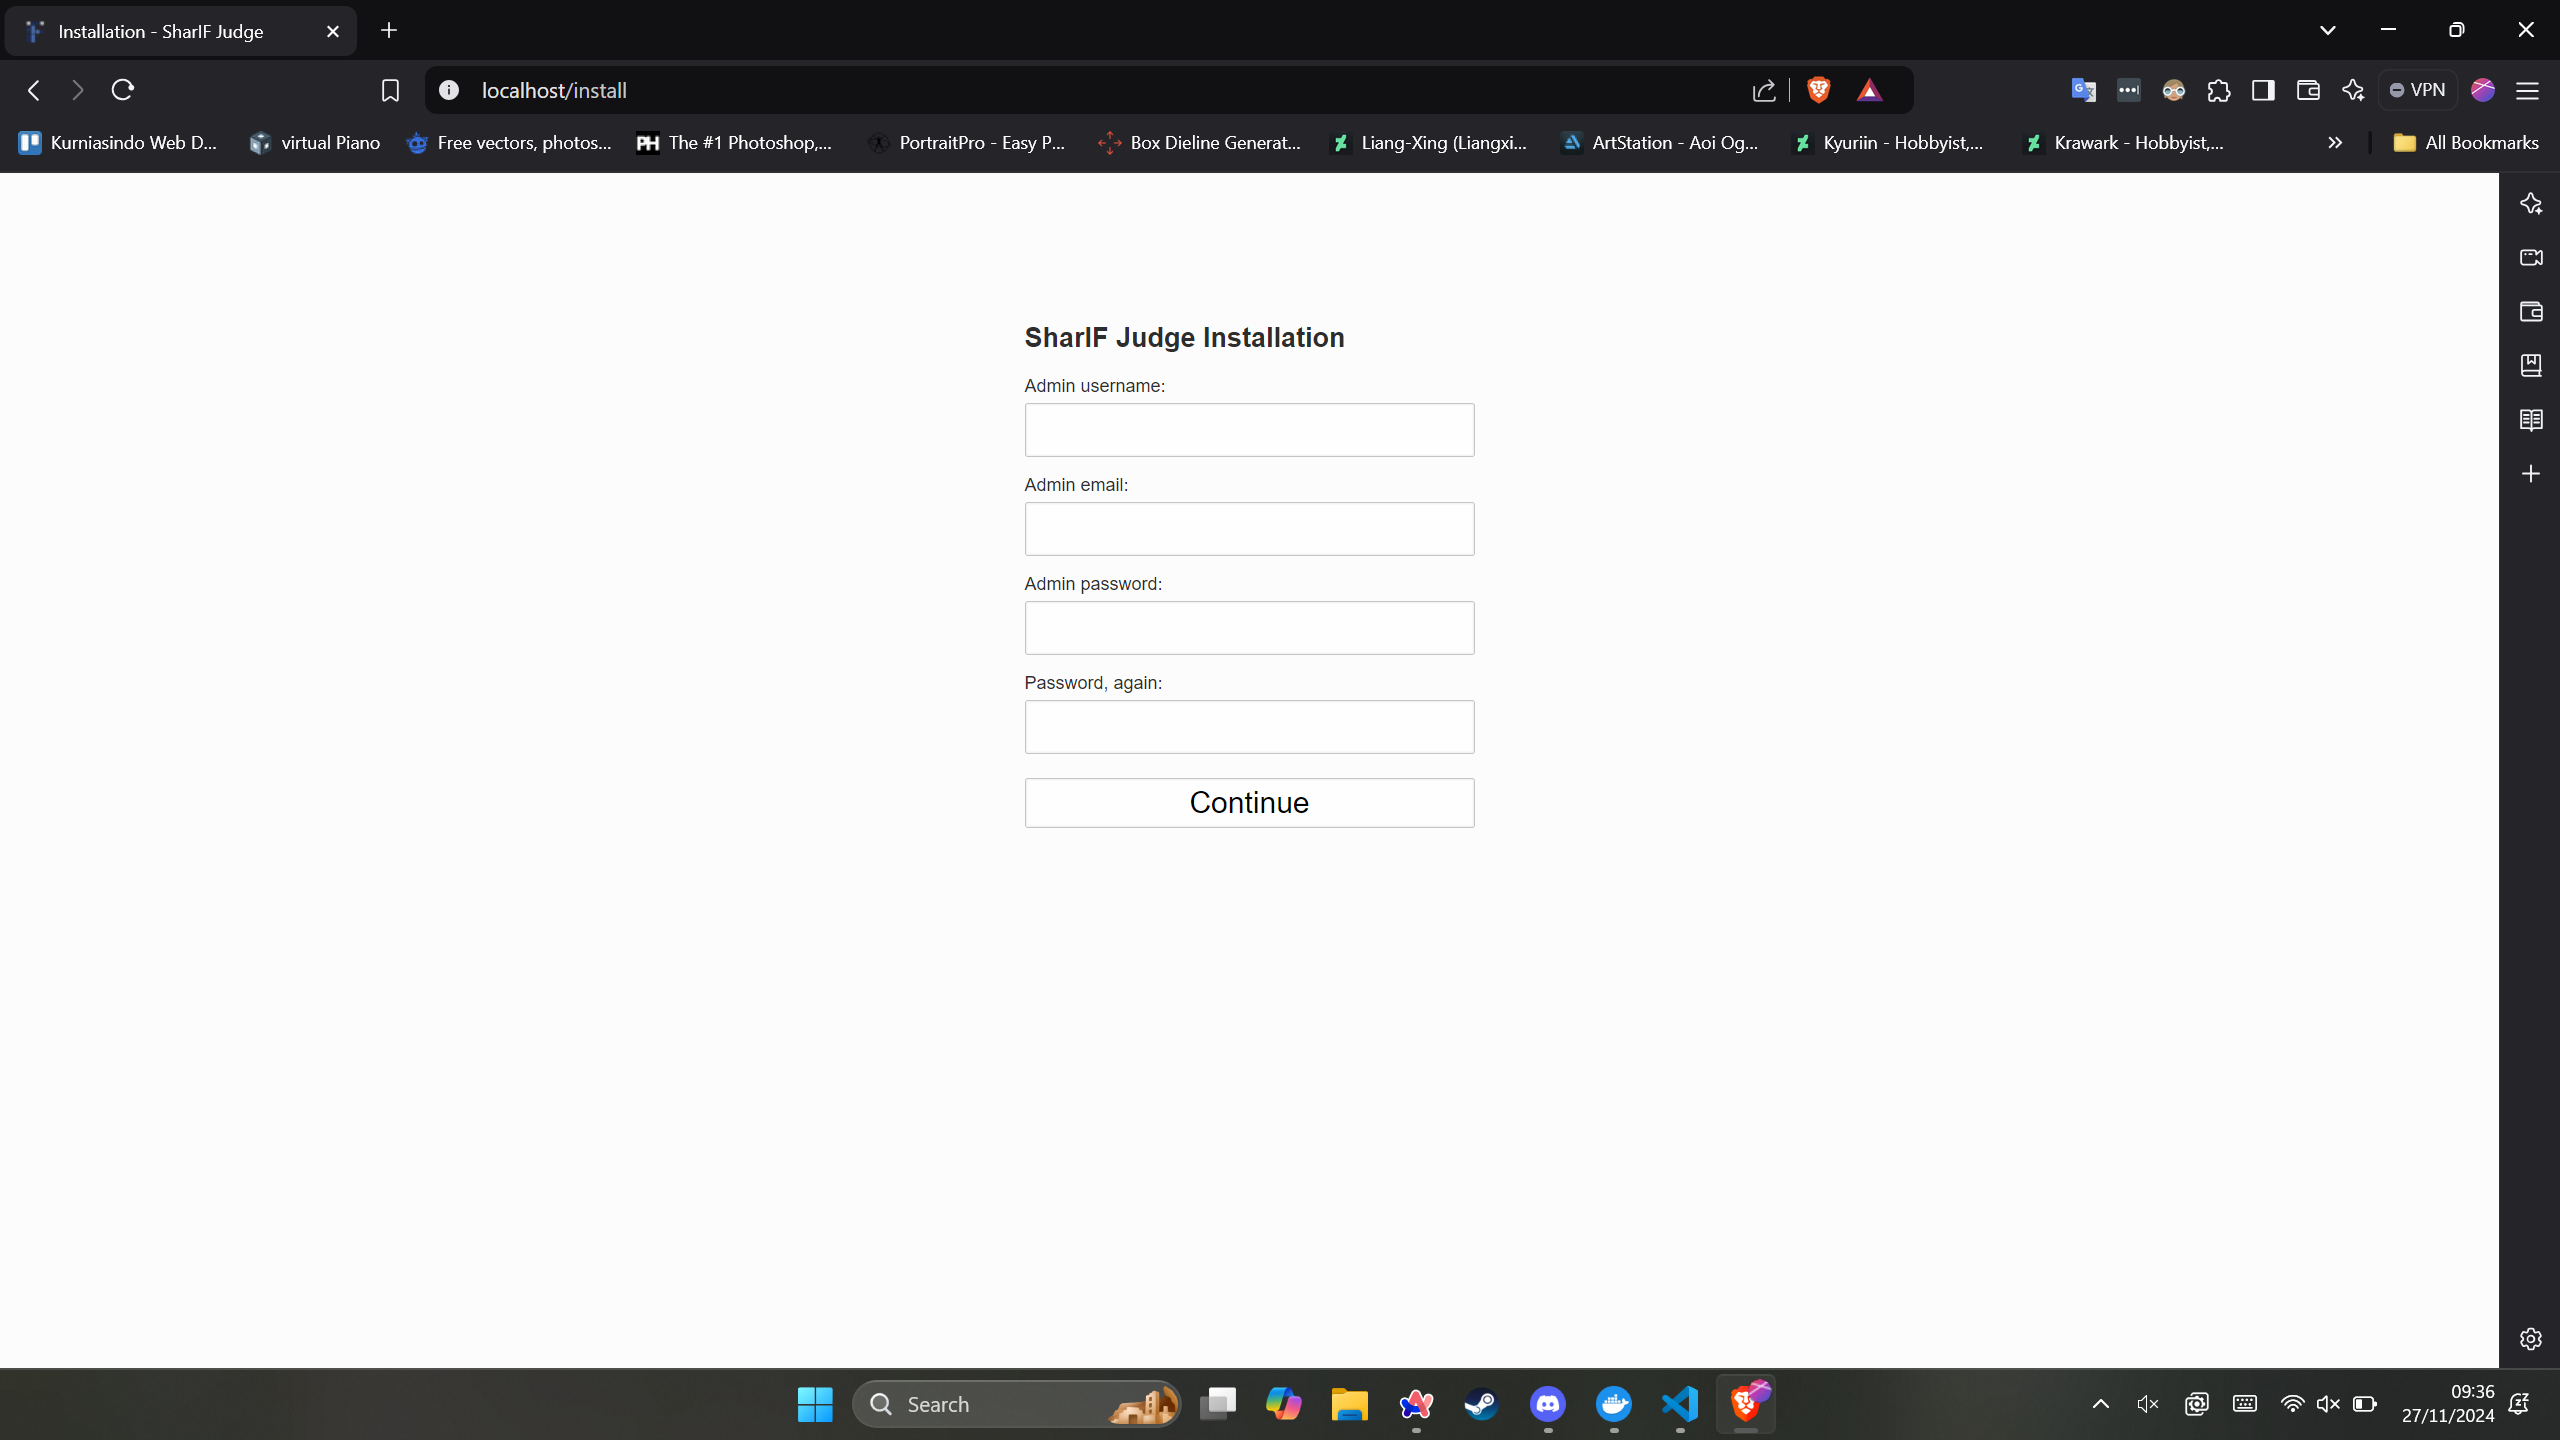
\includegraphics[width=\textwidth]{views/install.png}
		      \caption{Halaman Install}
		      \label{fig:3:1:1:install}
	      \end{figure}

	      Gambar \ref{fig:3:1:1:install} menunjukkan halaman Install. Pada halaman ini terdapat form untuk memperbaharui \textit{detail user admin}.

	\item Login %controller
	      \begin{figure}[H]
		      \centering
		      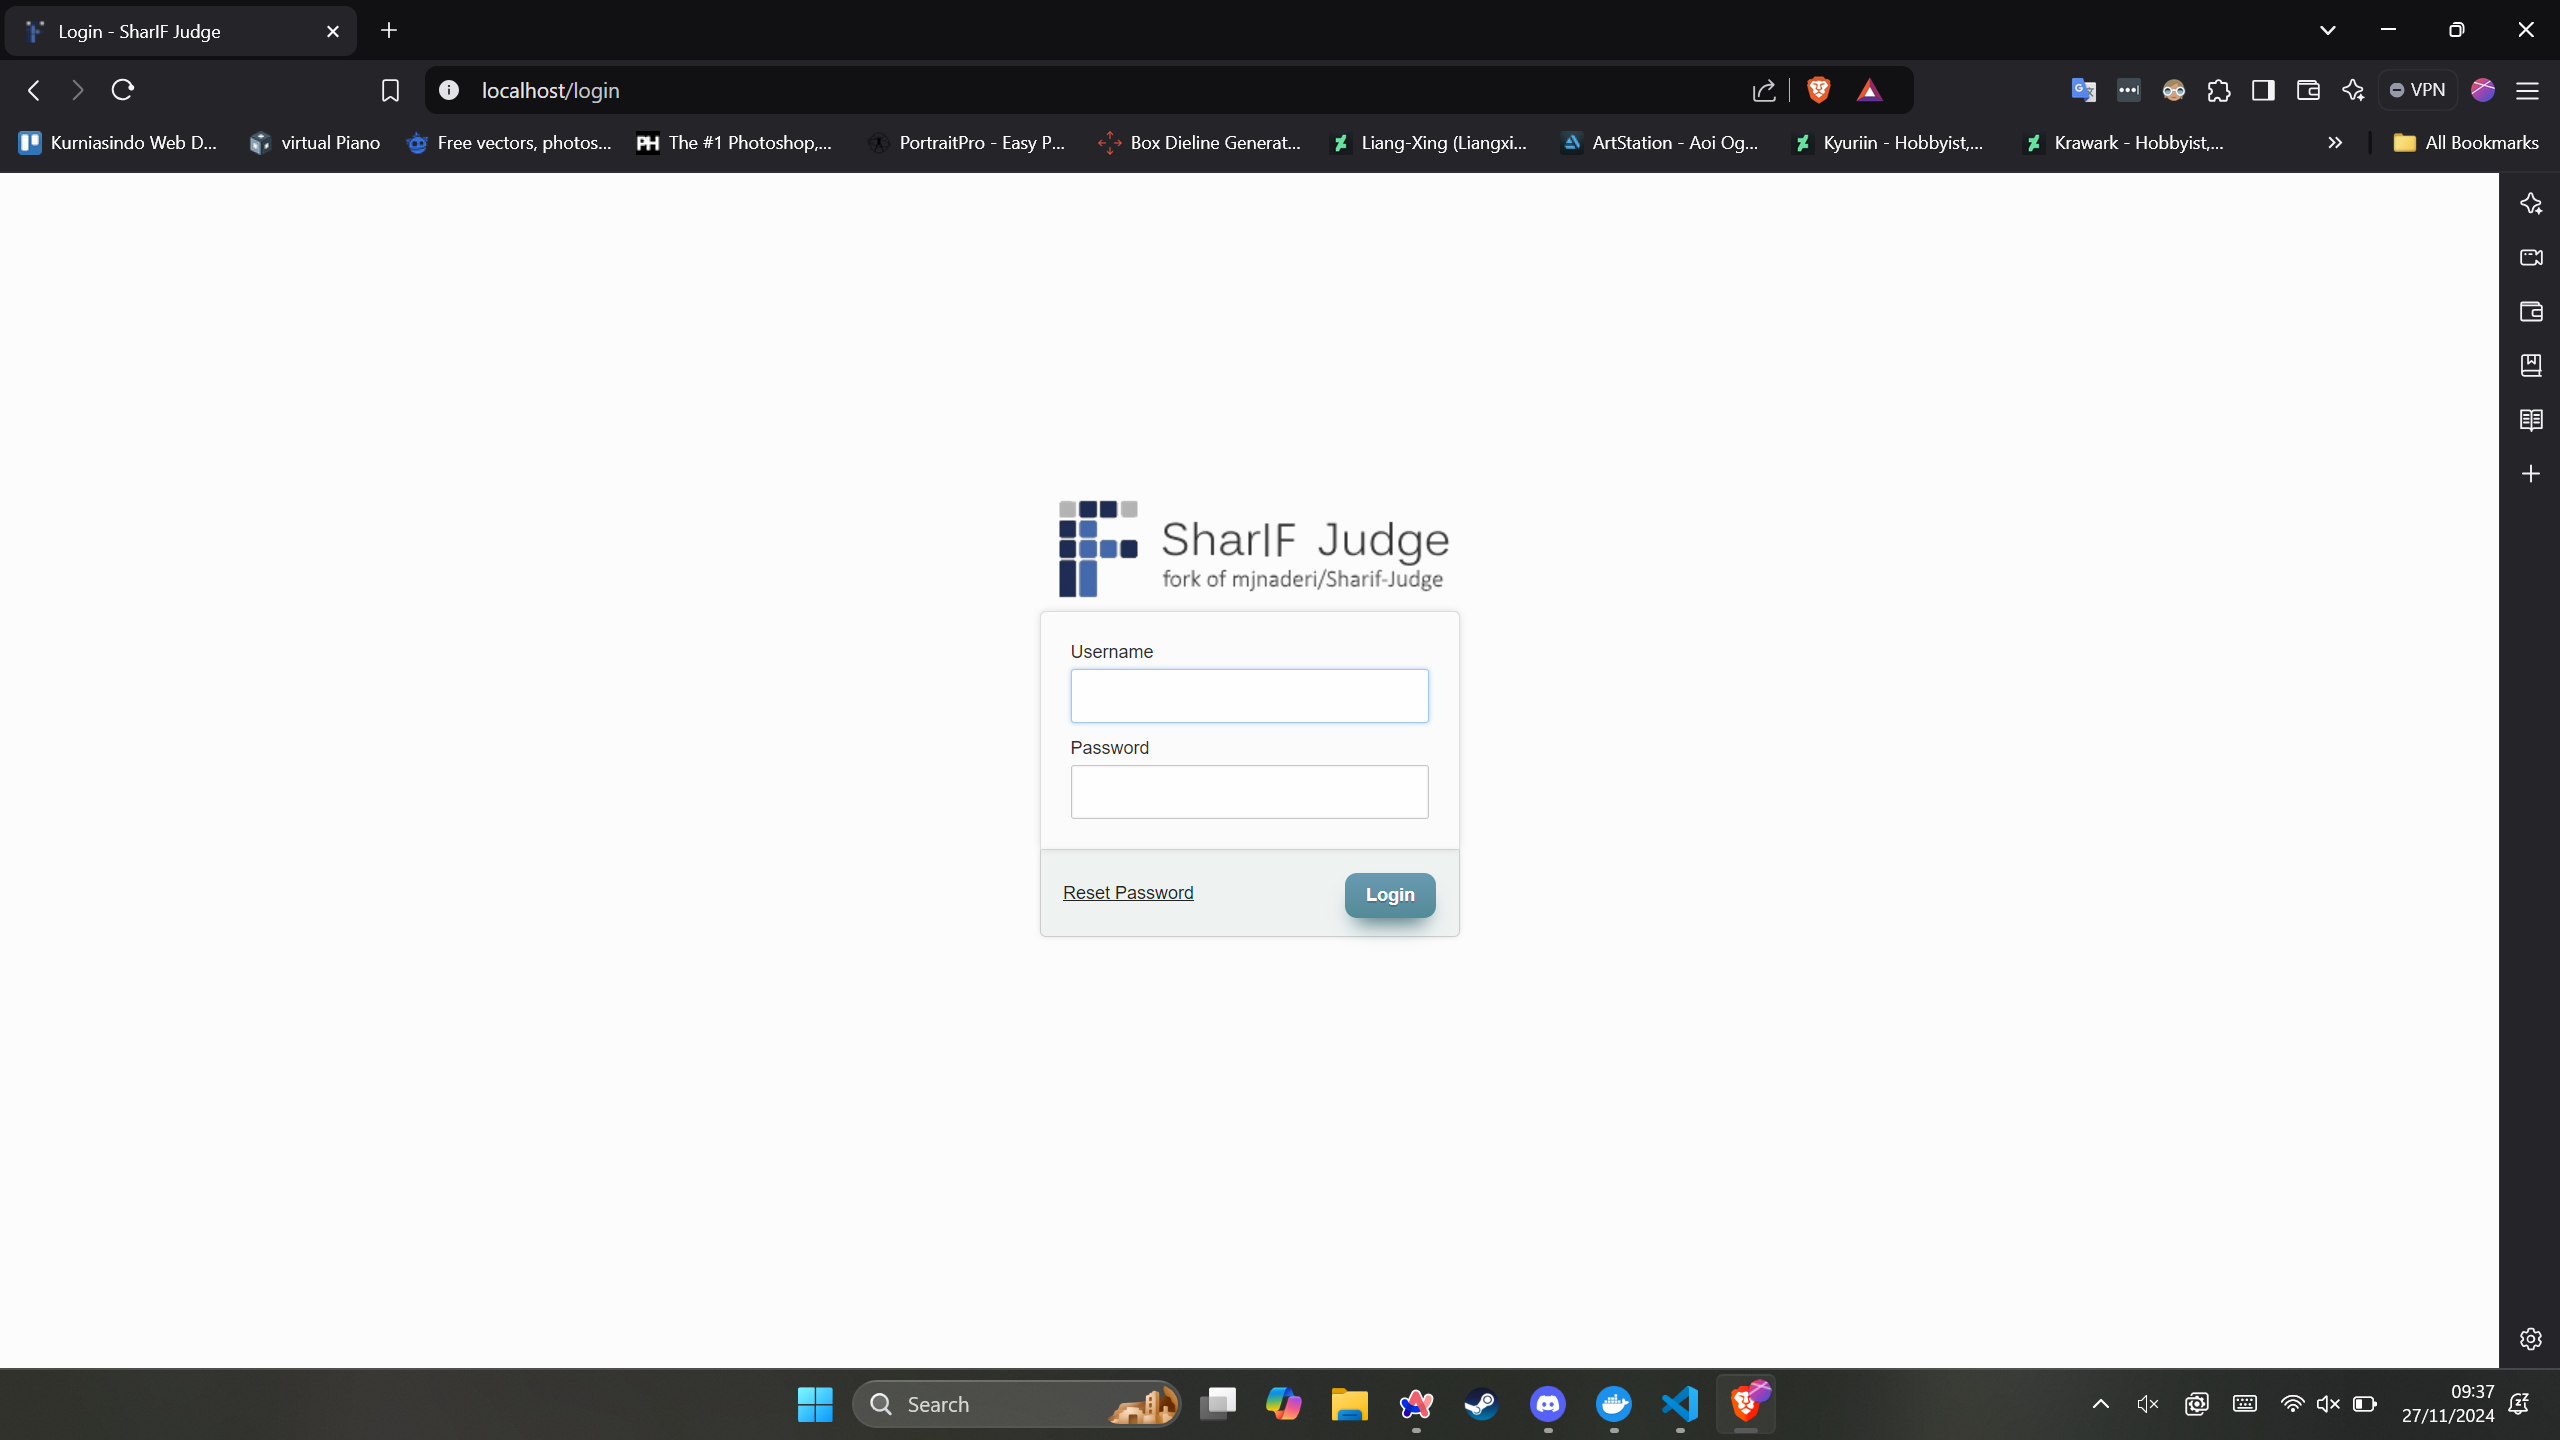
\includegraphics[width=\textwidth]{views/login.png}
		      \caption{Halaman Login}
		      \label{fig:3:1:1:login}
	      \end{figure}

	      Gambar \ref{fig:3:1:1:login} menunjukkan halaman Login.
	\item Dashboard %controller
	      \begin{figure}[H]
		      \centering
		      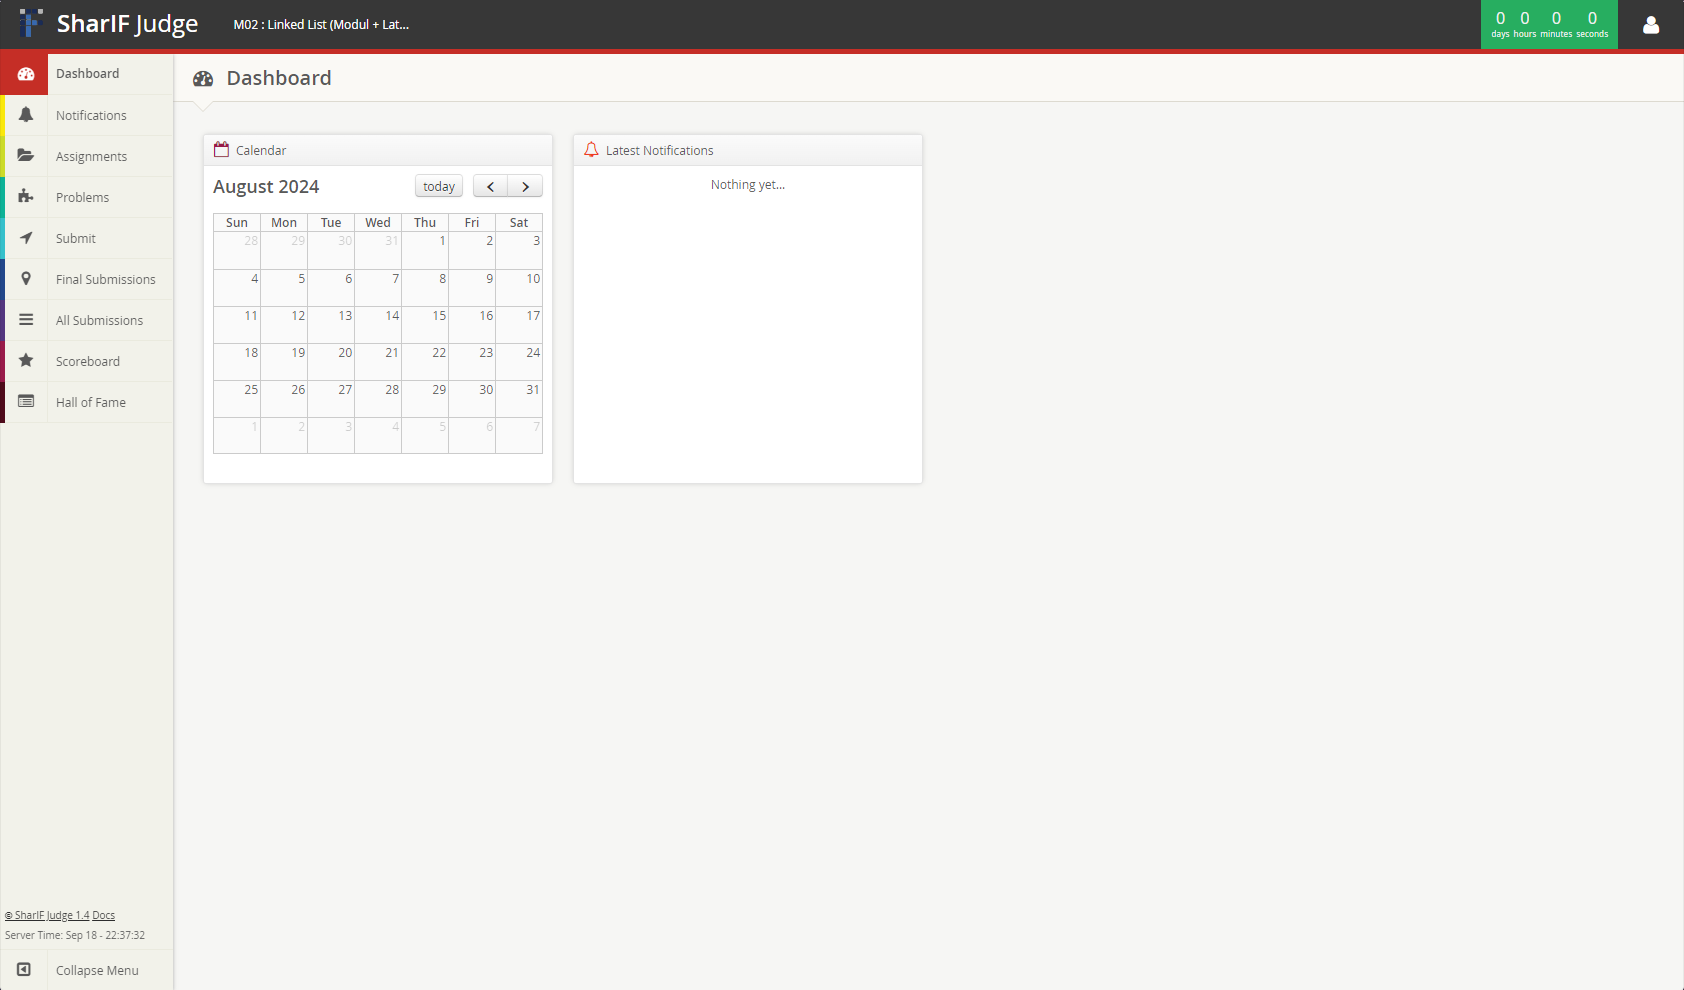
\includegraphics[width=\textwidth]{views/dashboard.png}
		      \caption{Halaman Dashboard}
		      \label{fig:3:1:1:dashboard}
	      \end{figure}

	      Gambar \ref{fig:3:1:1:dashboard} menunjukkan halaman Dashboard yang dapat diakses oleh semua \textit{role}.

	\item Settings %controller
	      \begin{figure}[H]
		      \centering
		      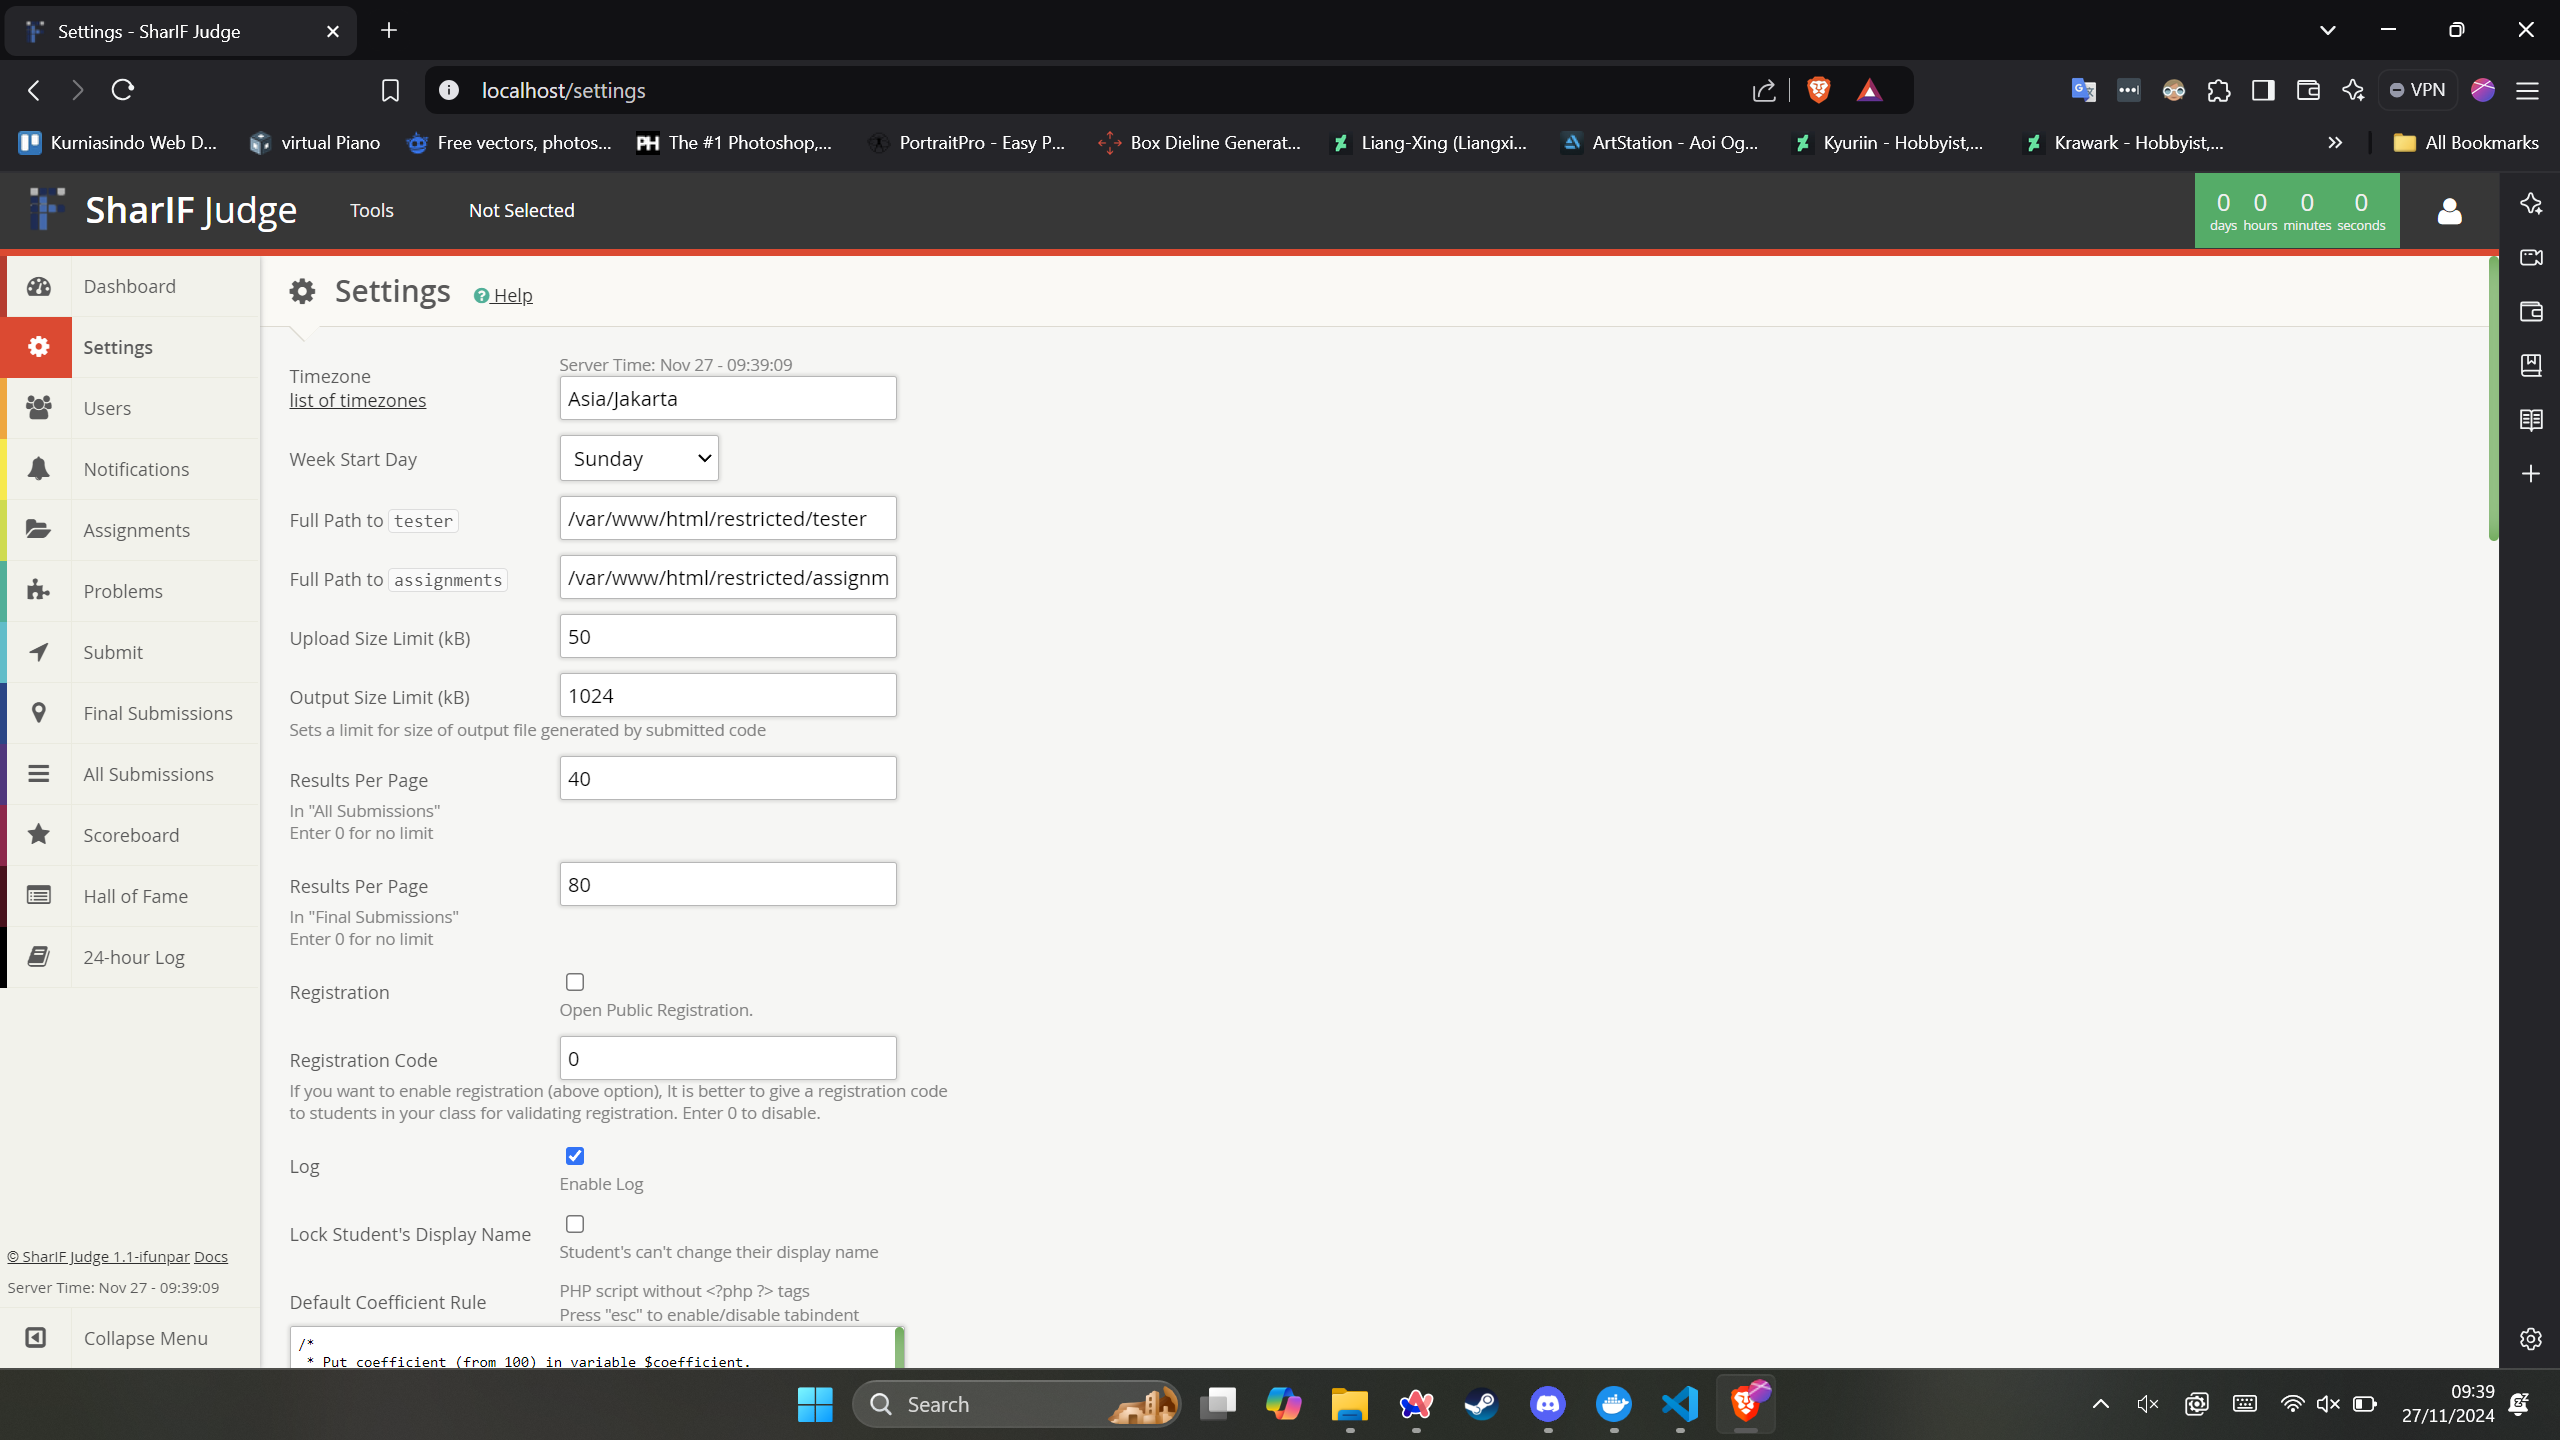
\includegraphics[width=\textwidth]{views/settings.png}
		      \caption{Halaman Settings}
		      \label{fig:3:1:1:settings}
	      \end{figure}

	      Gambar \ref{fig:3:1:1:settings} menunjukkan halaman Users yang hanya dapat di akses oleh \textit{role admin} dan \textit{head instructor}.

	\item User %controller
	      \begin{figure}[H]
		      \centering
		      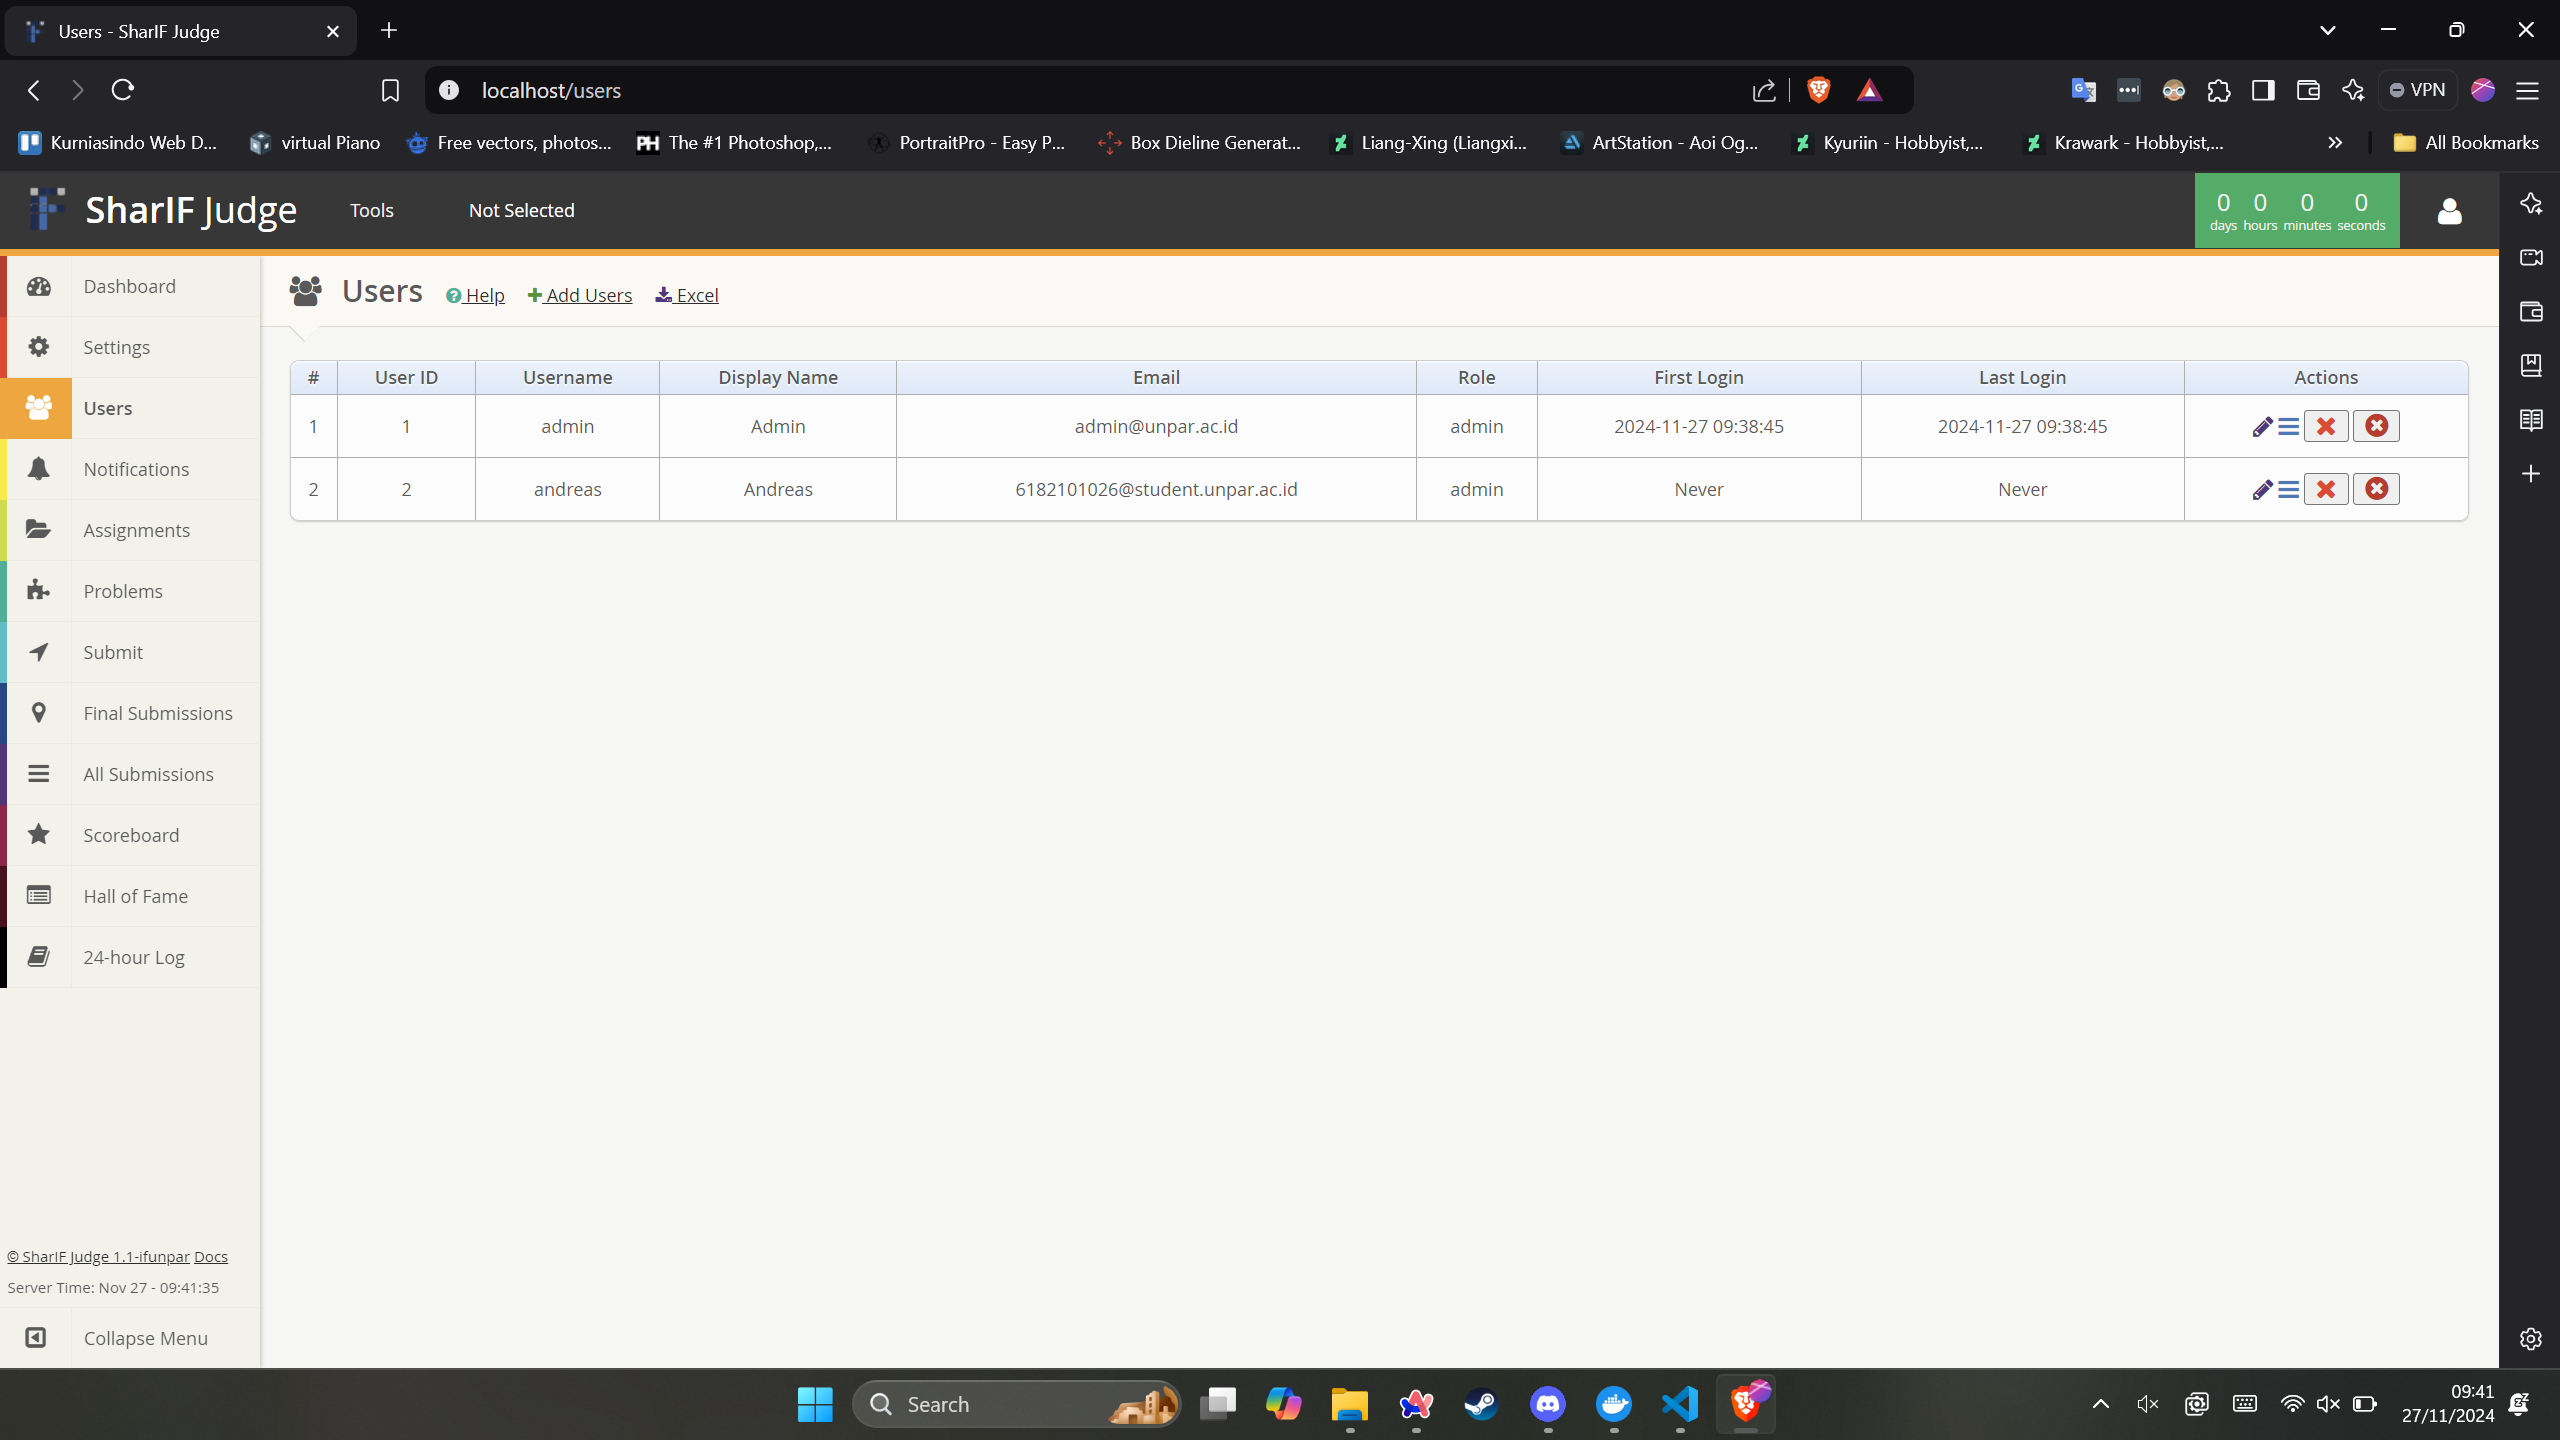
\includegraphics[width=\textwidth]{views/users.png}
		      \caption{Halaman Users}
		      \label{fig:3:1:1:users}
	      \end{figure}

	      Gambar \ref{fig:3:1:1:users} menunjukkan halaman Users. Pada halaman ini terdapat daftar seluruh \textit{user} yang terdaftar pada SharIF Judge. Pengguna dapat membuat, memperbaharui, dan menghapus \textit{user}.

	\item Profile %controller
	      \begin{figure}[H]
		      \centering
		      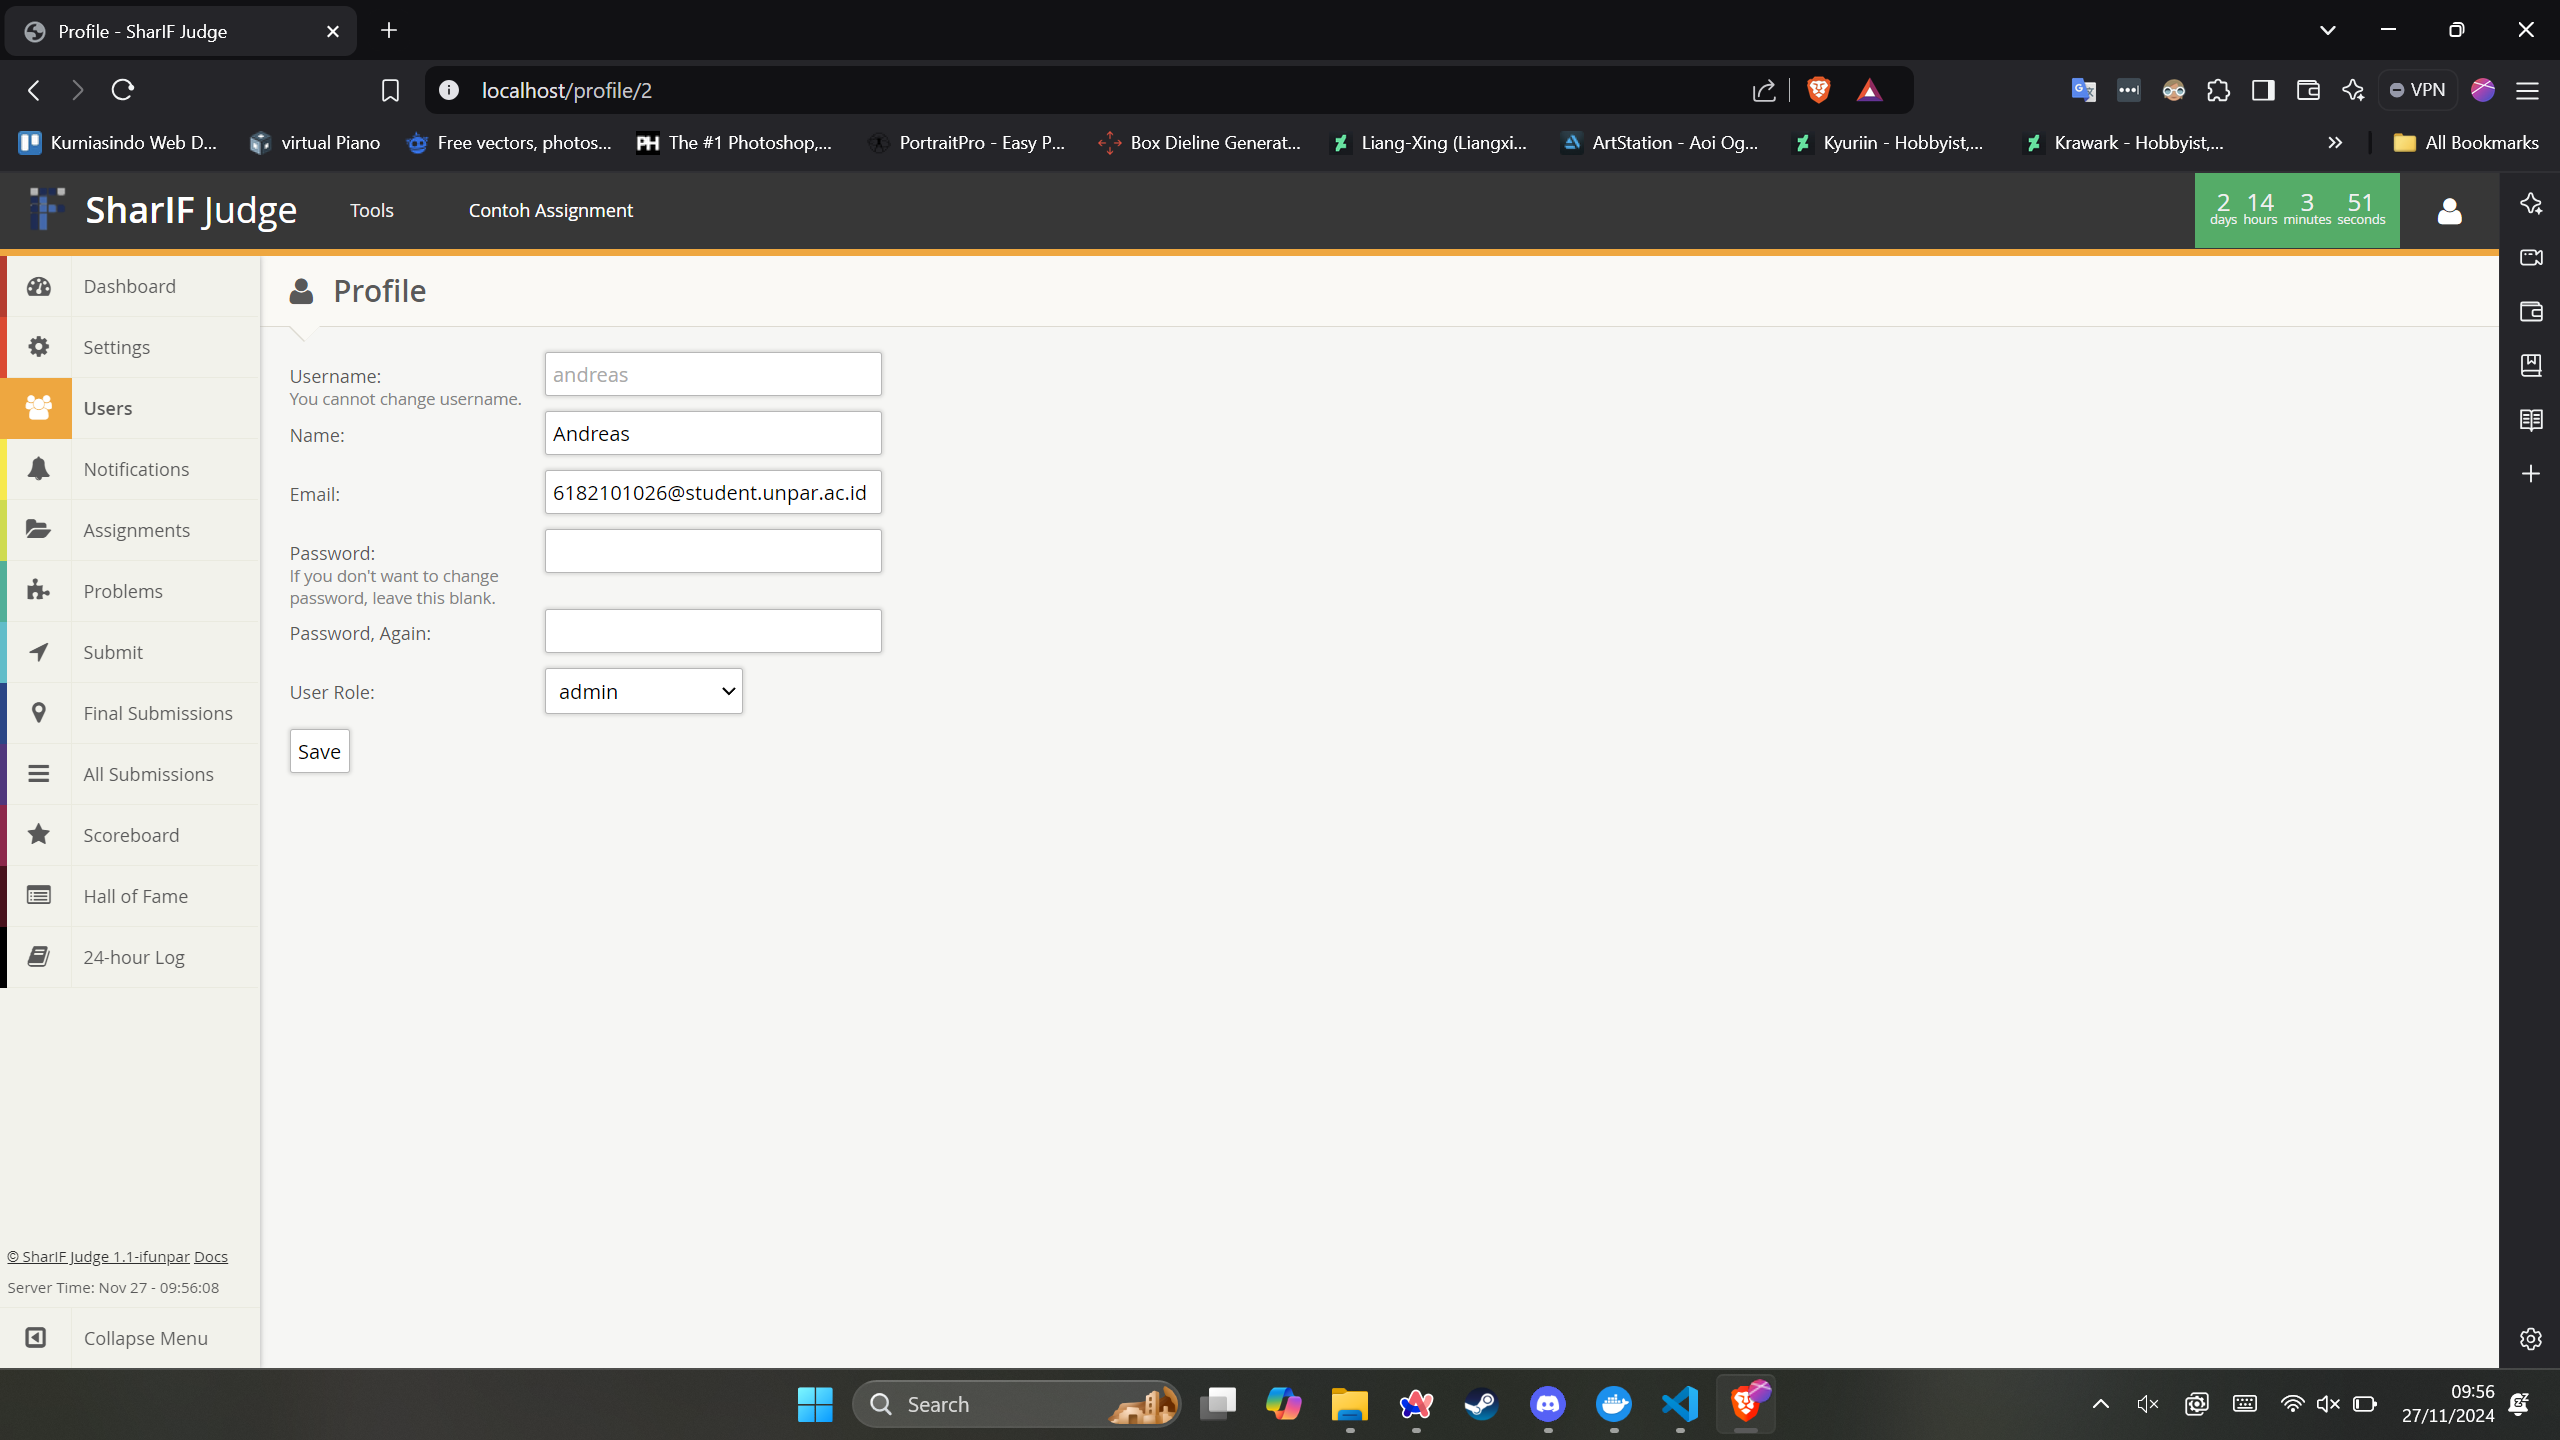
\includegraphics[width=\textwidth]{views/profile.png}
		      \caption{Halaman Profile}
		      \label{fig:3:1:1:profile}
	      \end{figure}

	      Gambar \ref{fig:3:1:1:profile} menunjukkan halaman Profile yang dapat di akses oleh semua \textit{role}. Tetapi ada fitur yang hanya dapat di akses oleh \textit{role admin} dan \textit{head instructor} yaitu pergantian role.

	\item Notifications %controller
	      % \begin{figure}[H]
	      %       \centering
	      %       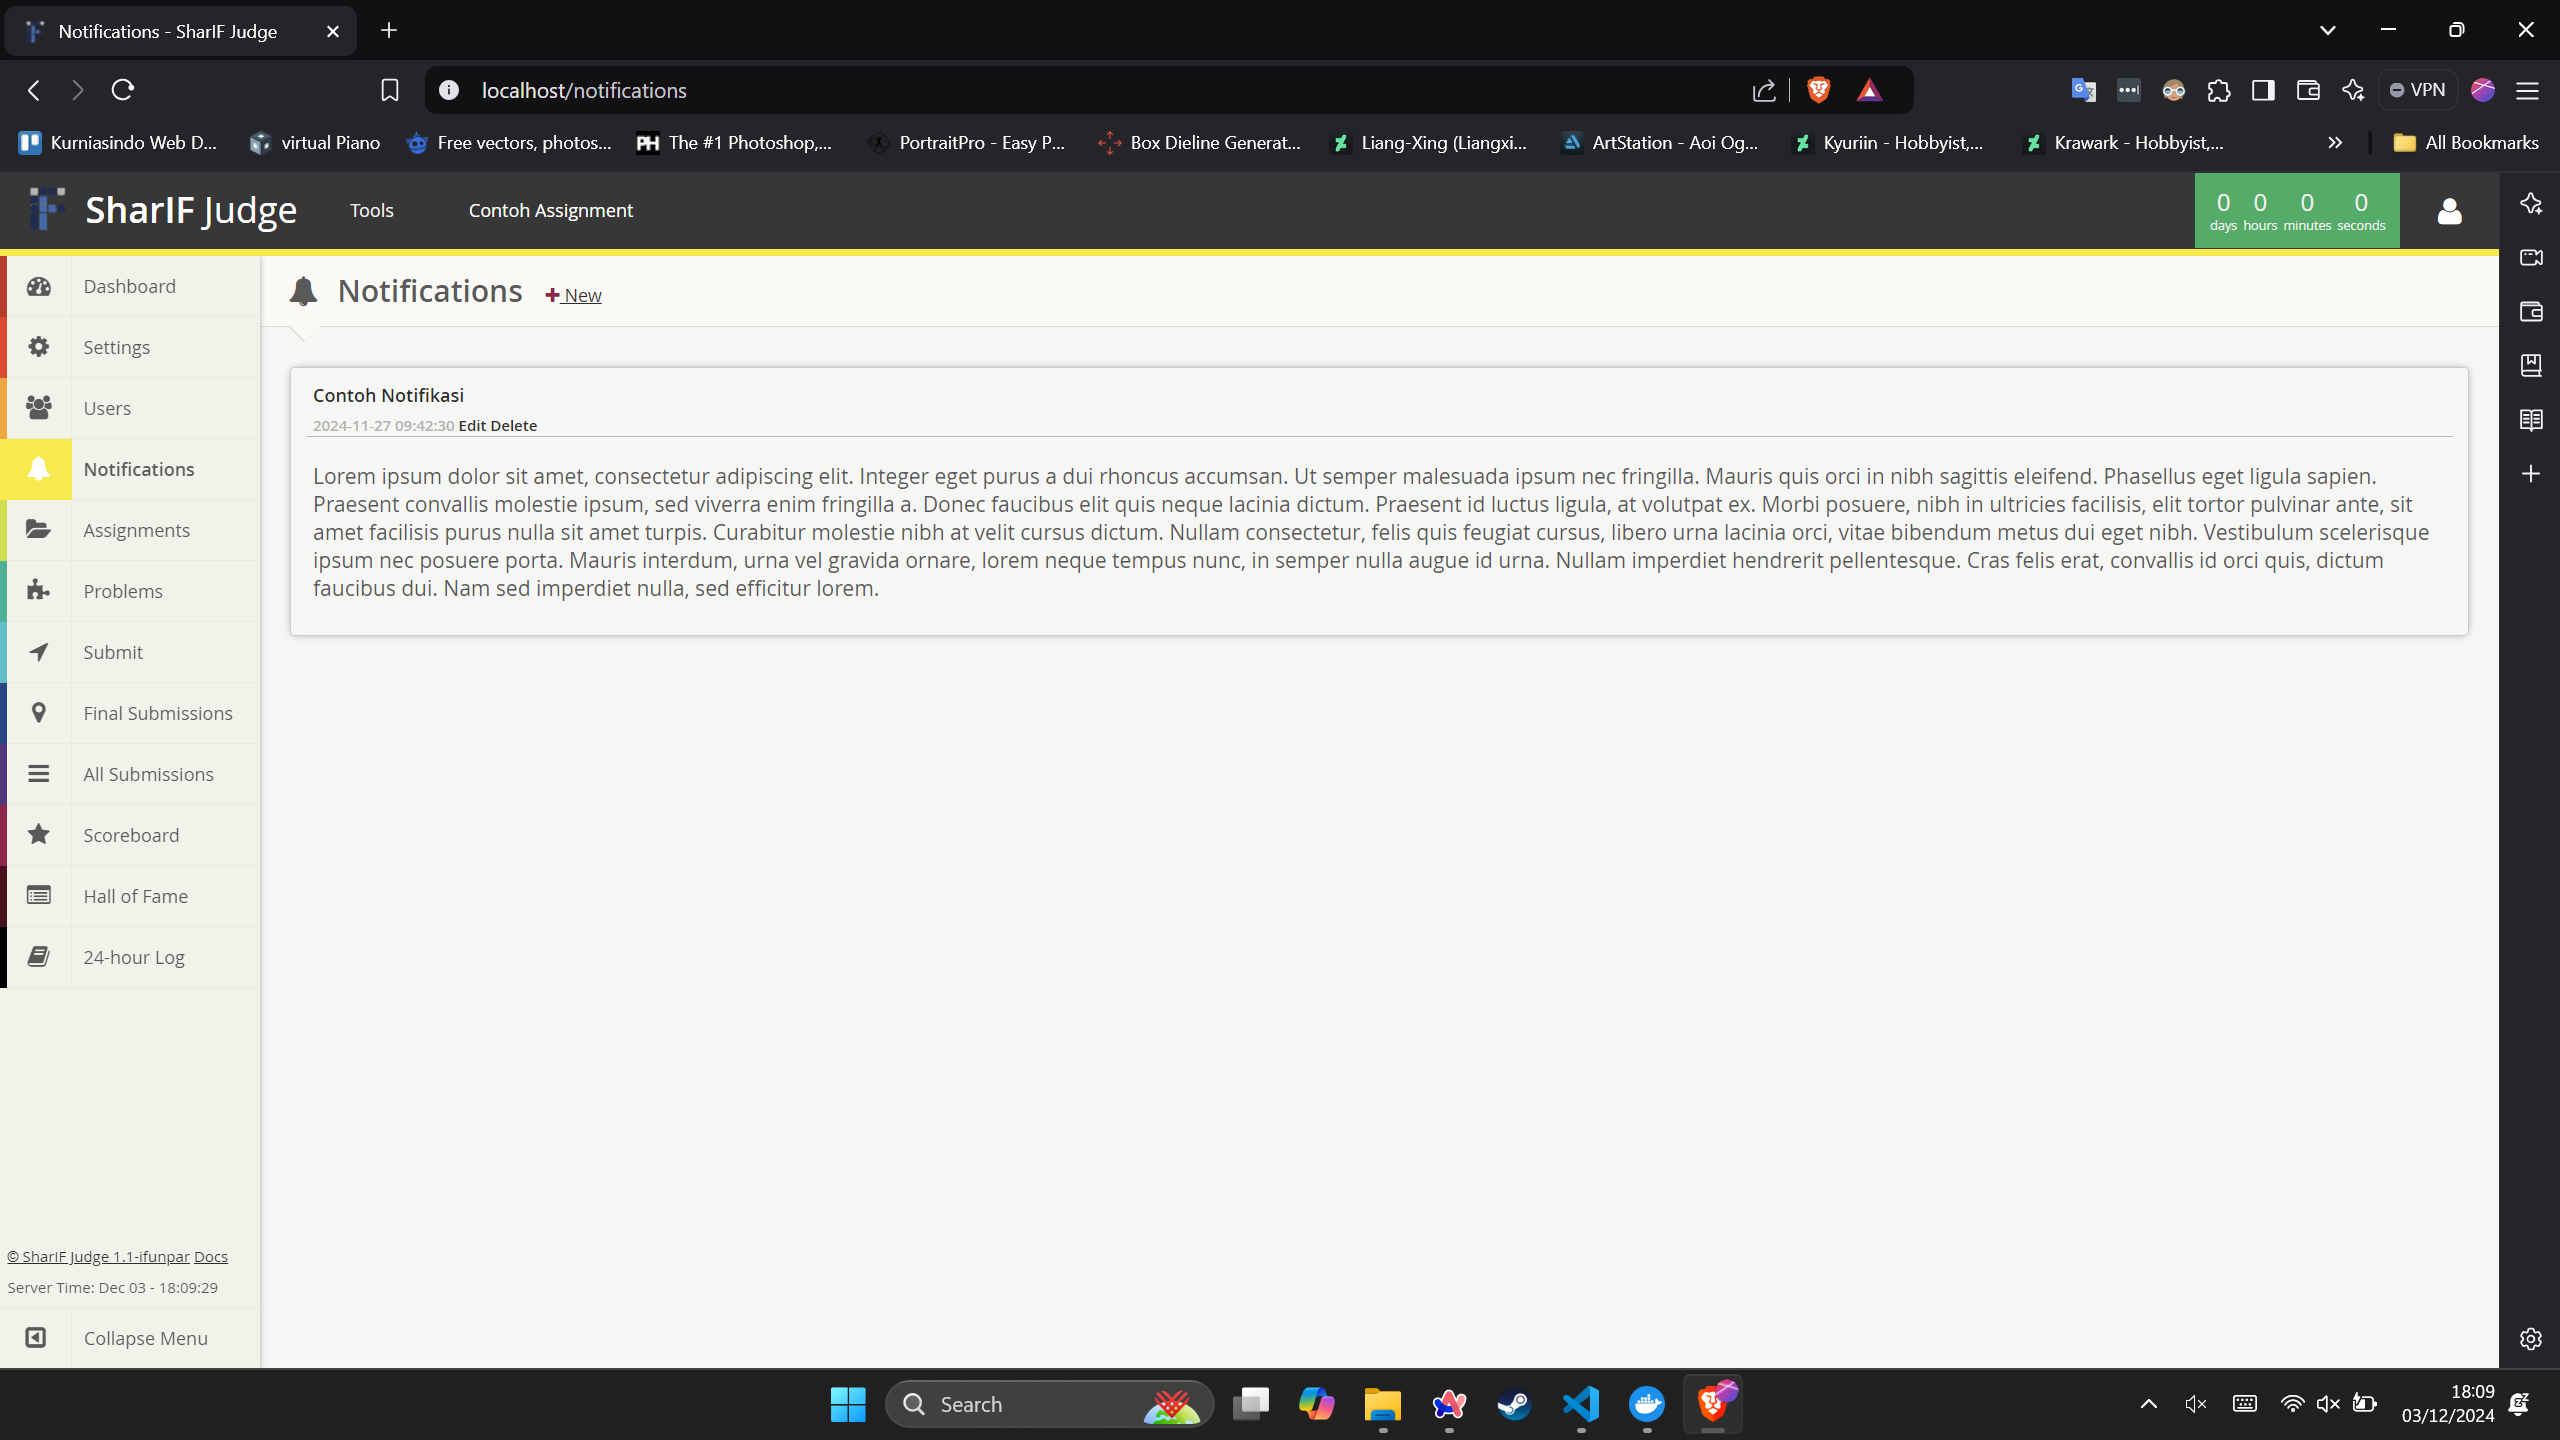
\includegraphics[width=\textwidth]{views/notifications.png}
	      %       \caption{Halaman Notifications}
	      %       \label{fig:3:1:1:notif}
	      % \end{figure}

	      % Gambar \ref{fig:3:1:1:notif} menunjukkan halaman Notifikasi.
	\item Assignments %controller
	      \begin{figure}[H]
		      \centering
		      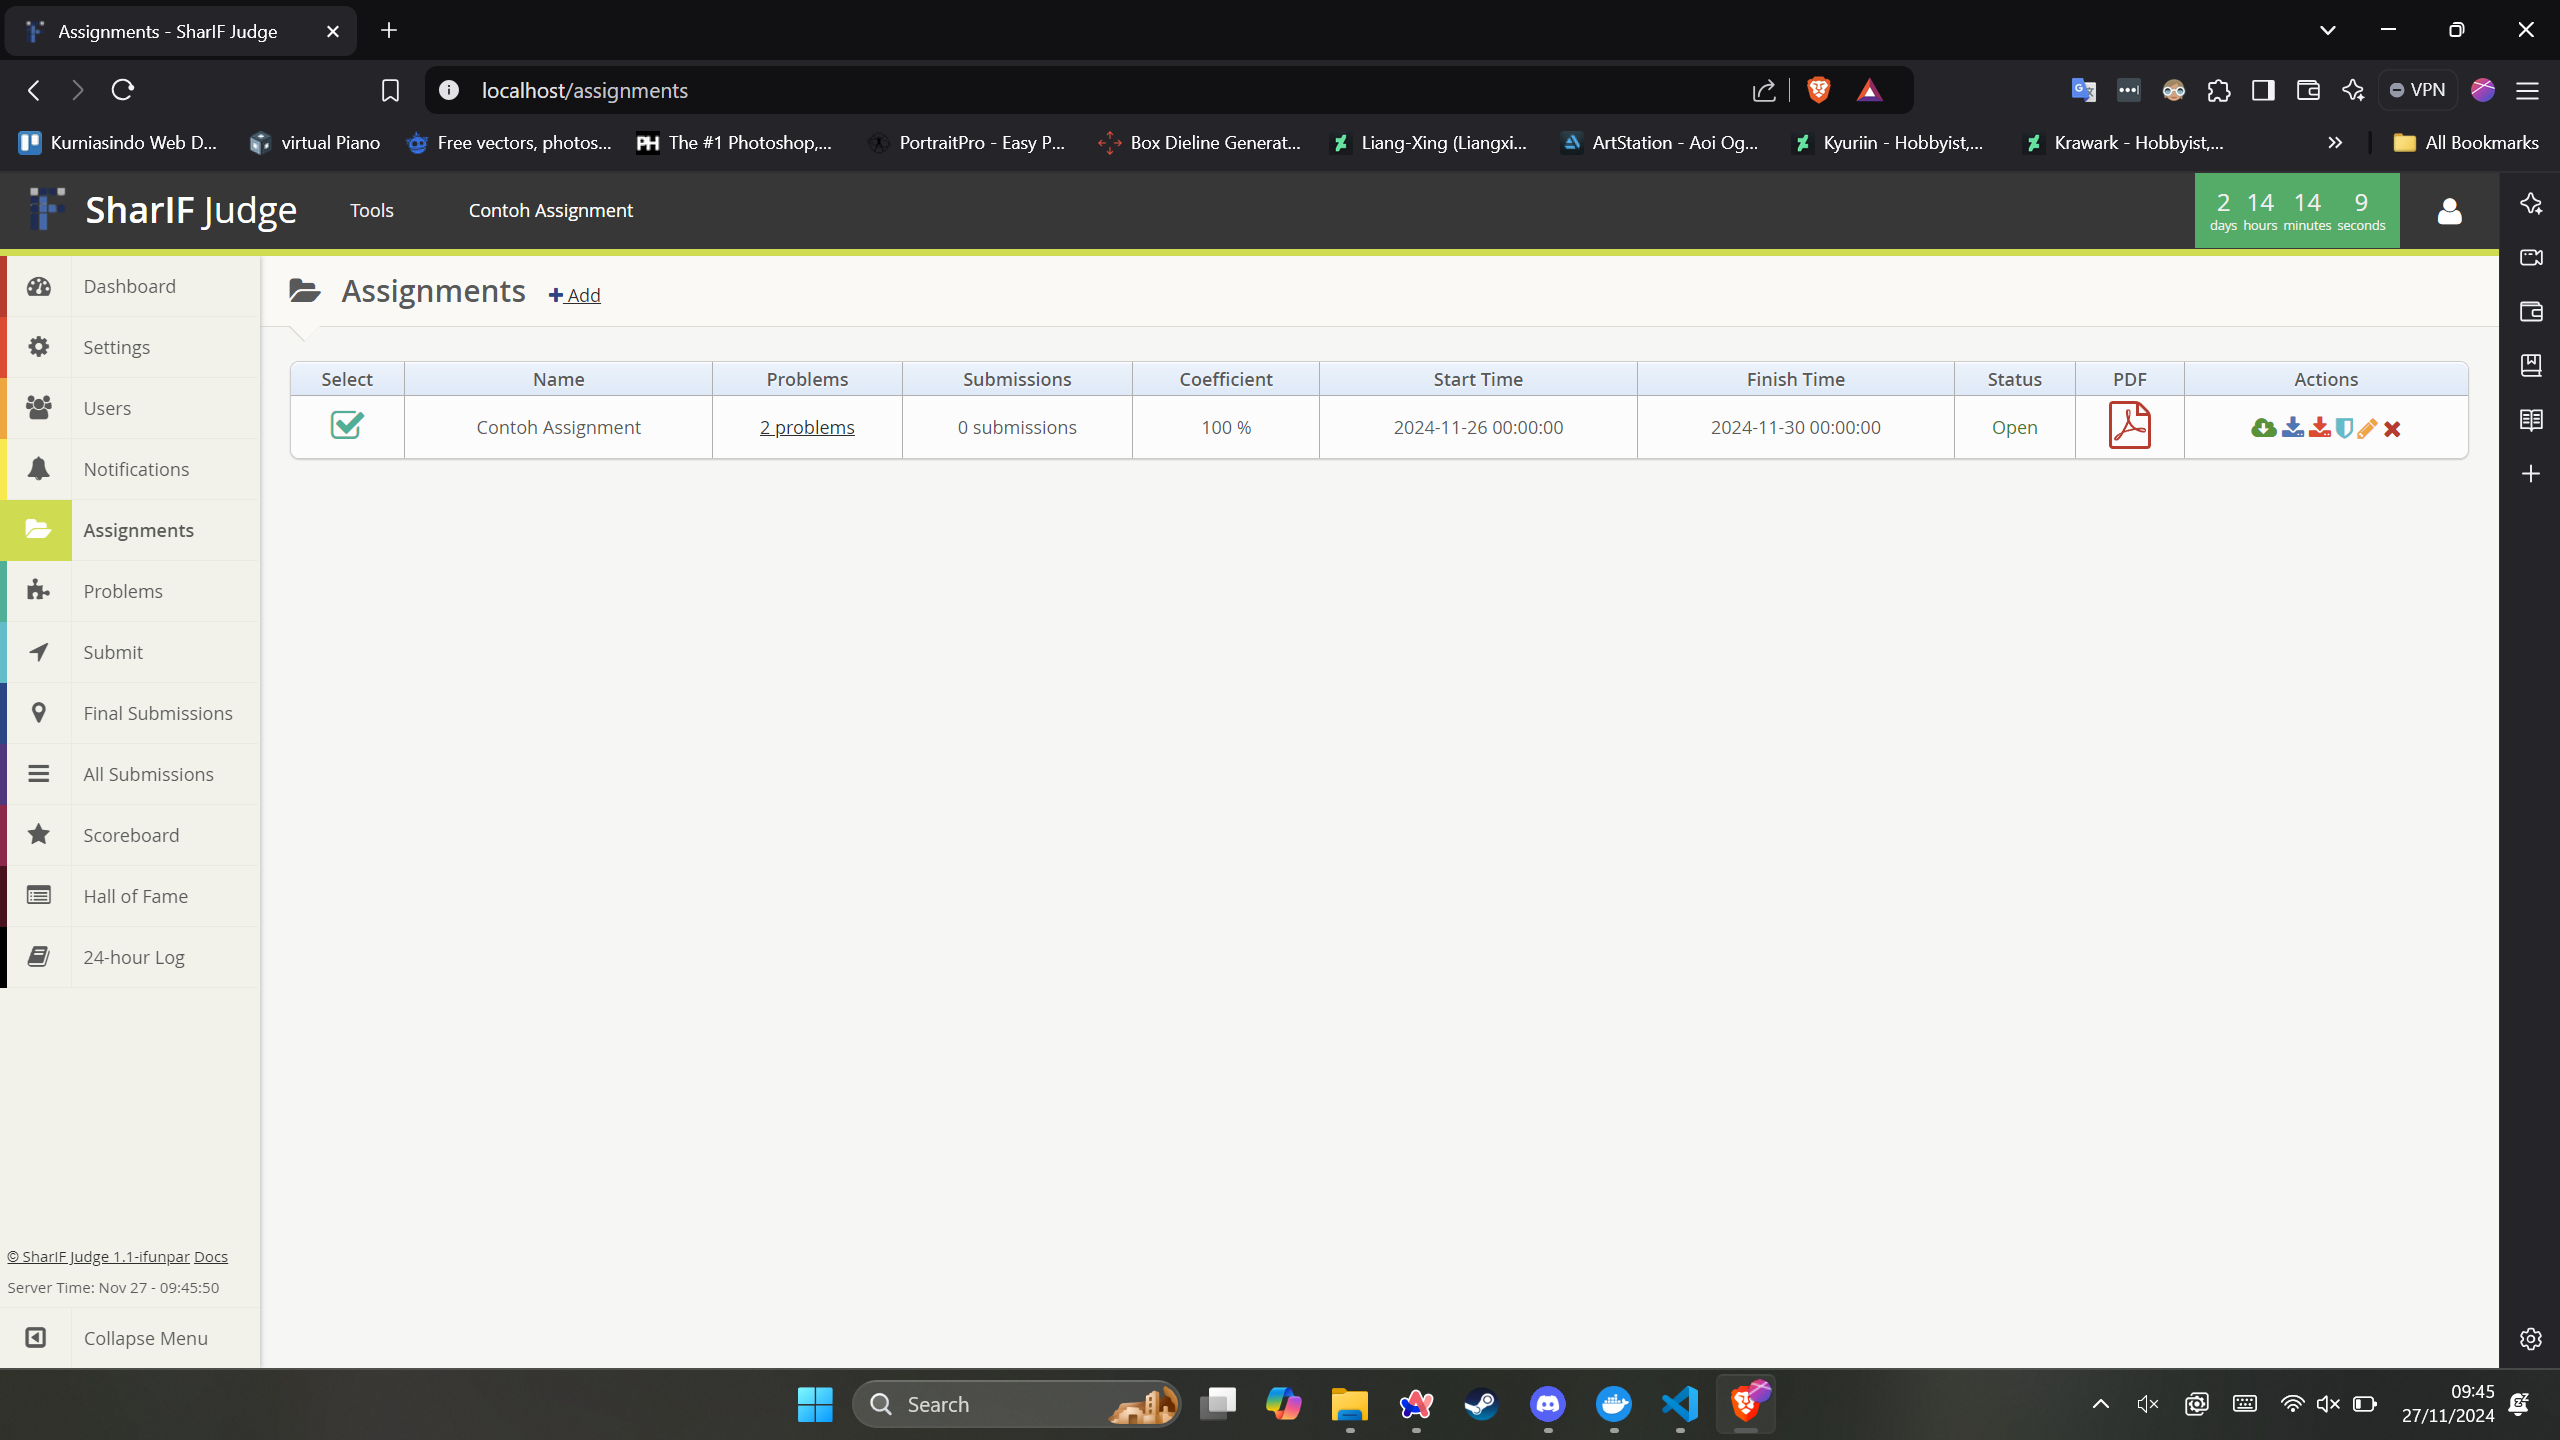
\includegraphics[width=\textwidth]{views/assignments.png}
		      \caption{Halaman Assignments}
		      \label{fig:3:1:1:assignments}
	      \end{figure}

	      Gambar \ref{fig:3:1:1:assignments} menunjukkan halaman Assignment. Pengguna dapat memilih assignment. Pada halaman ini terdapat \textit{actions} yang dibatasi akses oleh \textit{role} dapat dilihat \textit{actions} pada bab \ref{subs:2:1:users}.

	\item Rejudge %controller
	      \begin{figure}[H]
		      \centering
		      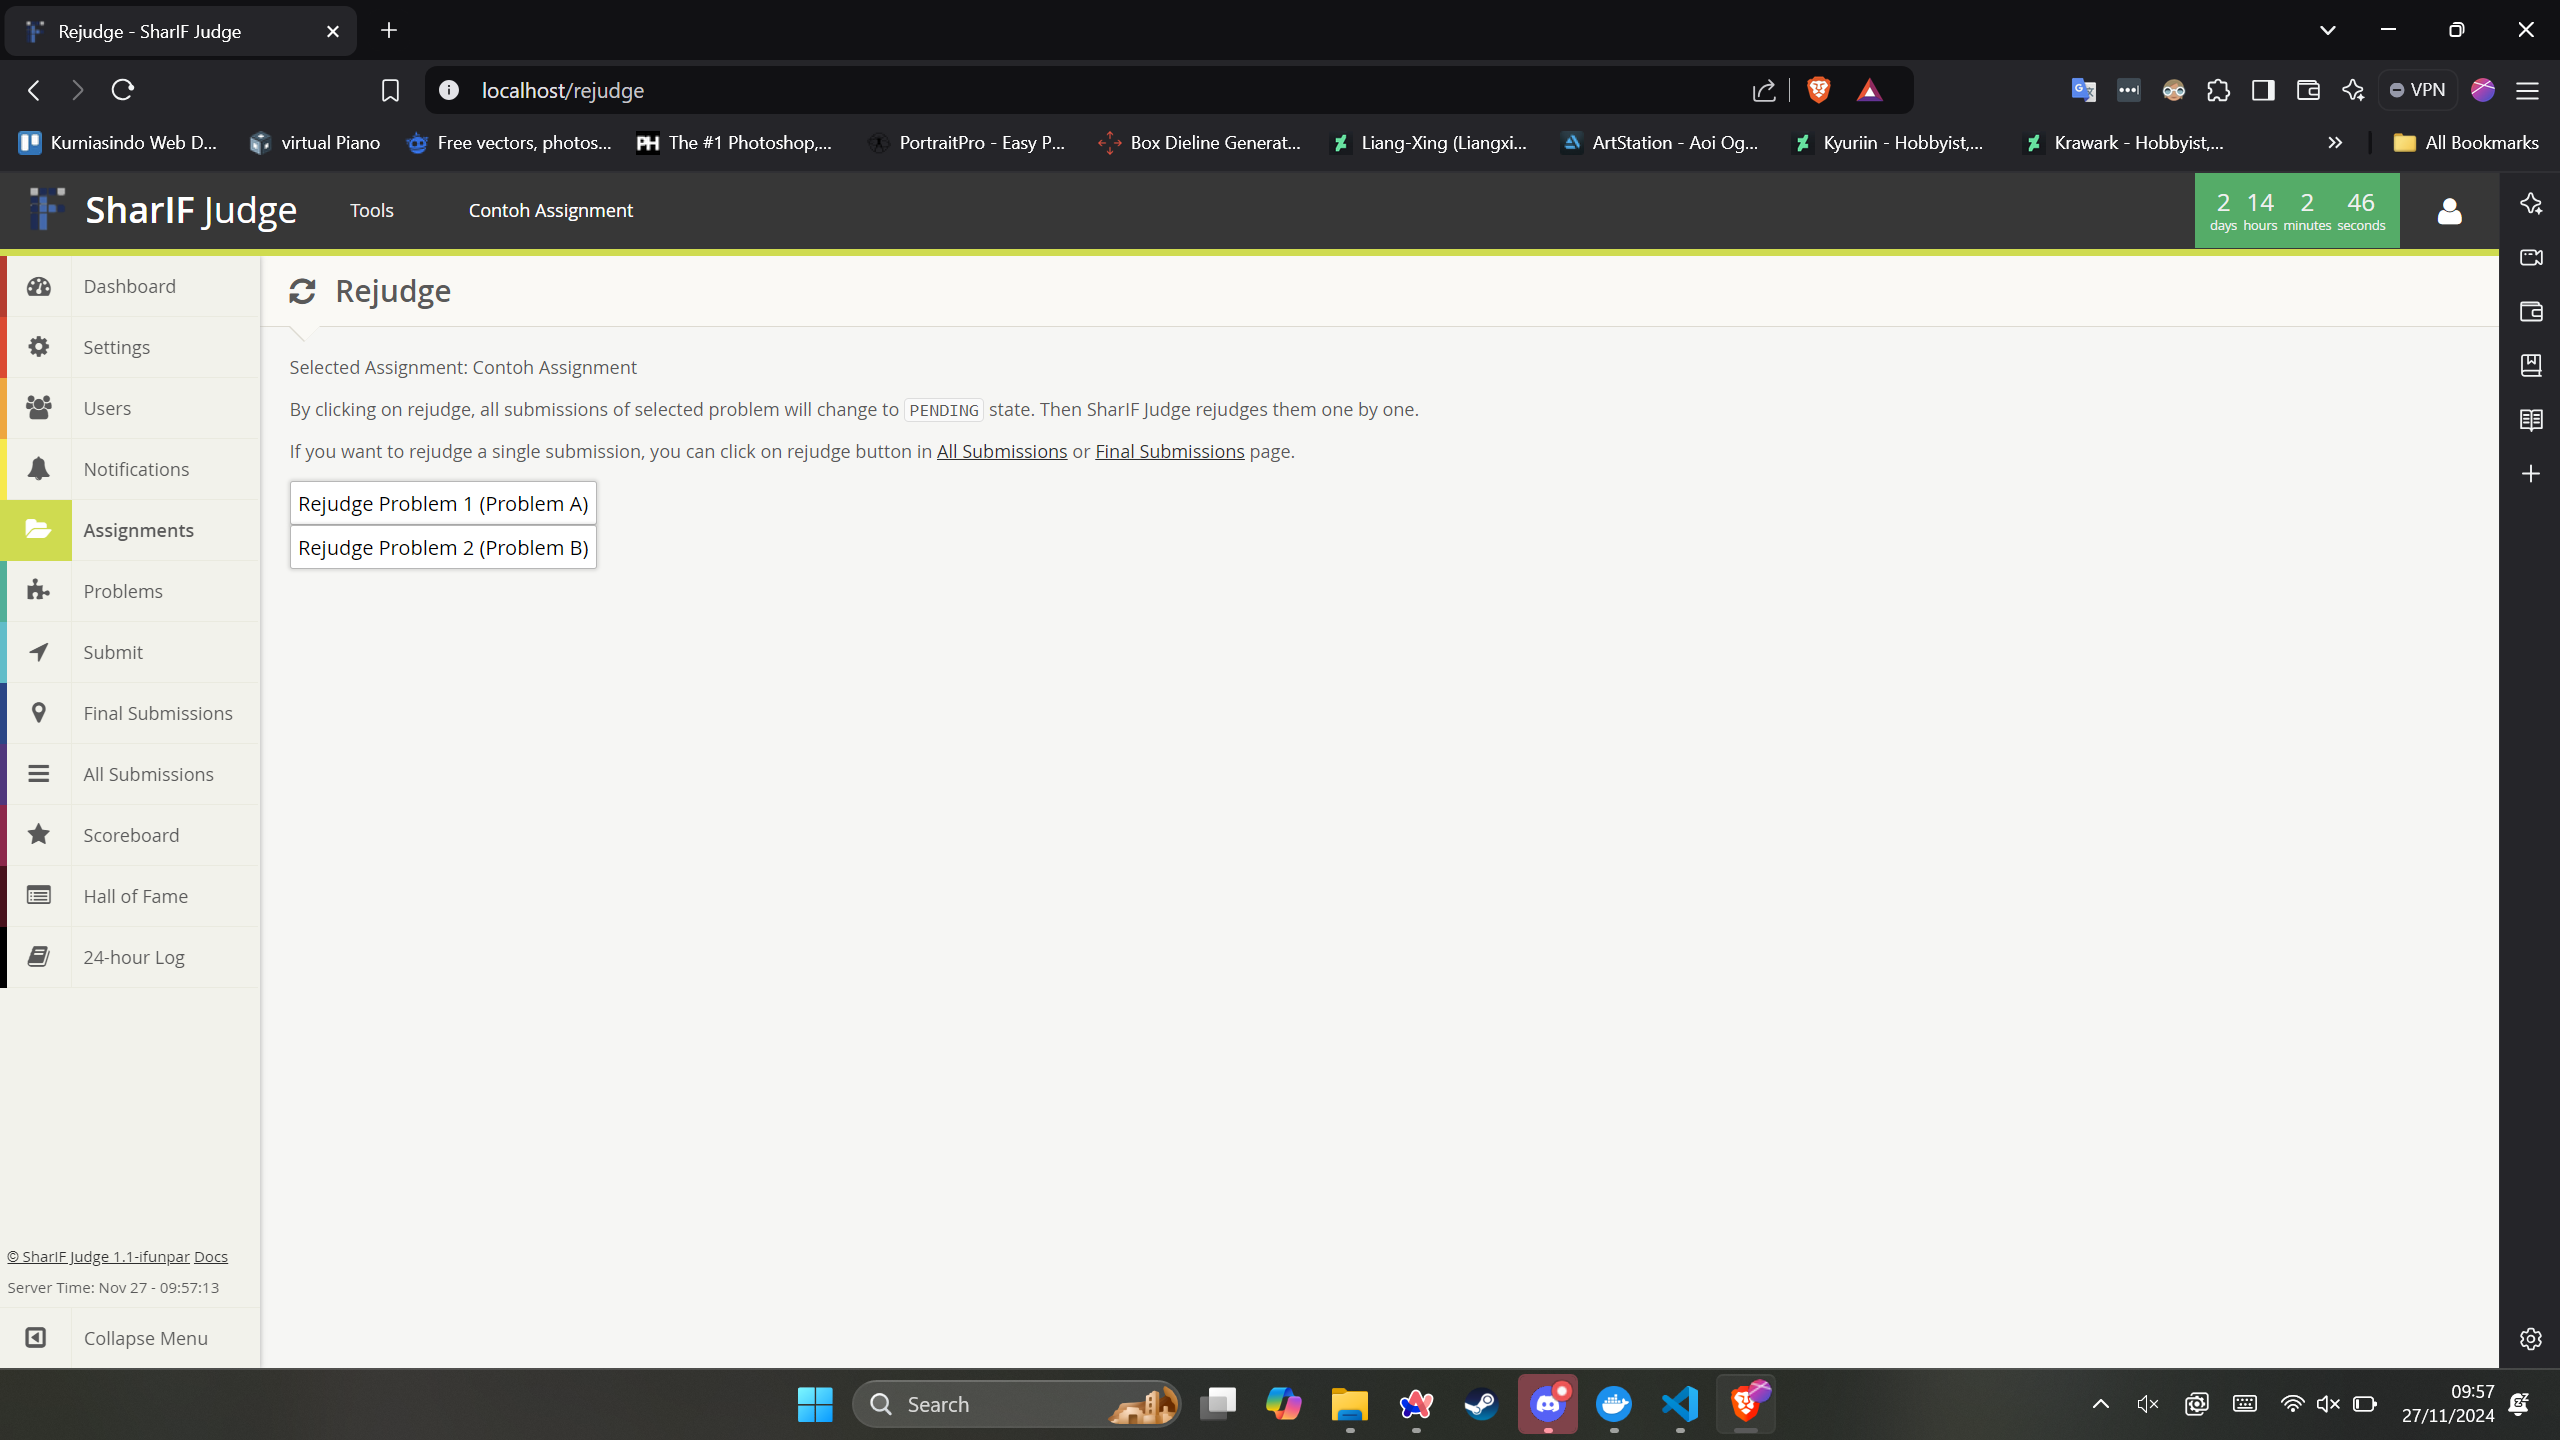
\includegraphics[width=\textwidth]{views/rejudge.png}
		      \caption{Halaman Rejudge}
		      \label{fig:3:1:1:rejudge}
	      \end{figure}

	      Gambar \ref{fig:3:1:1:rejudge} menunjukkan halaman Rejudge. Halaman ini hanya dapat di akses oleh \textit{role admin} dan \textit{head instructor}.

	\item Submission Queue %controller
	      % \begin{figure}[H]
	      %       \centering
	      %       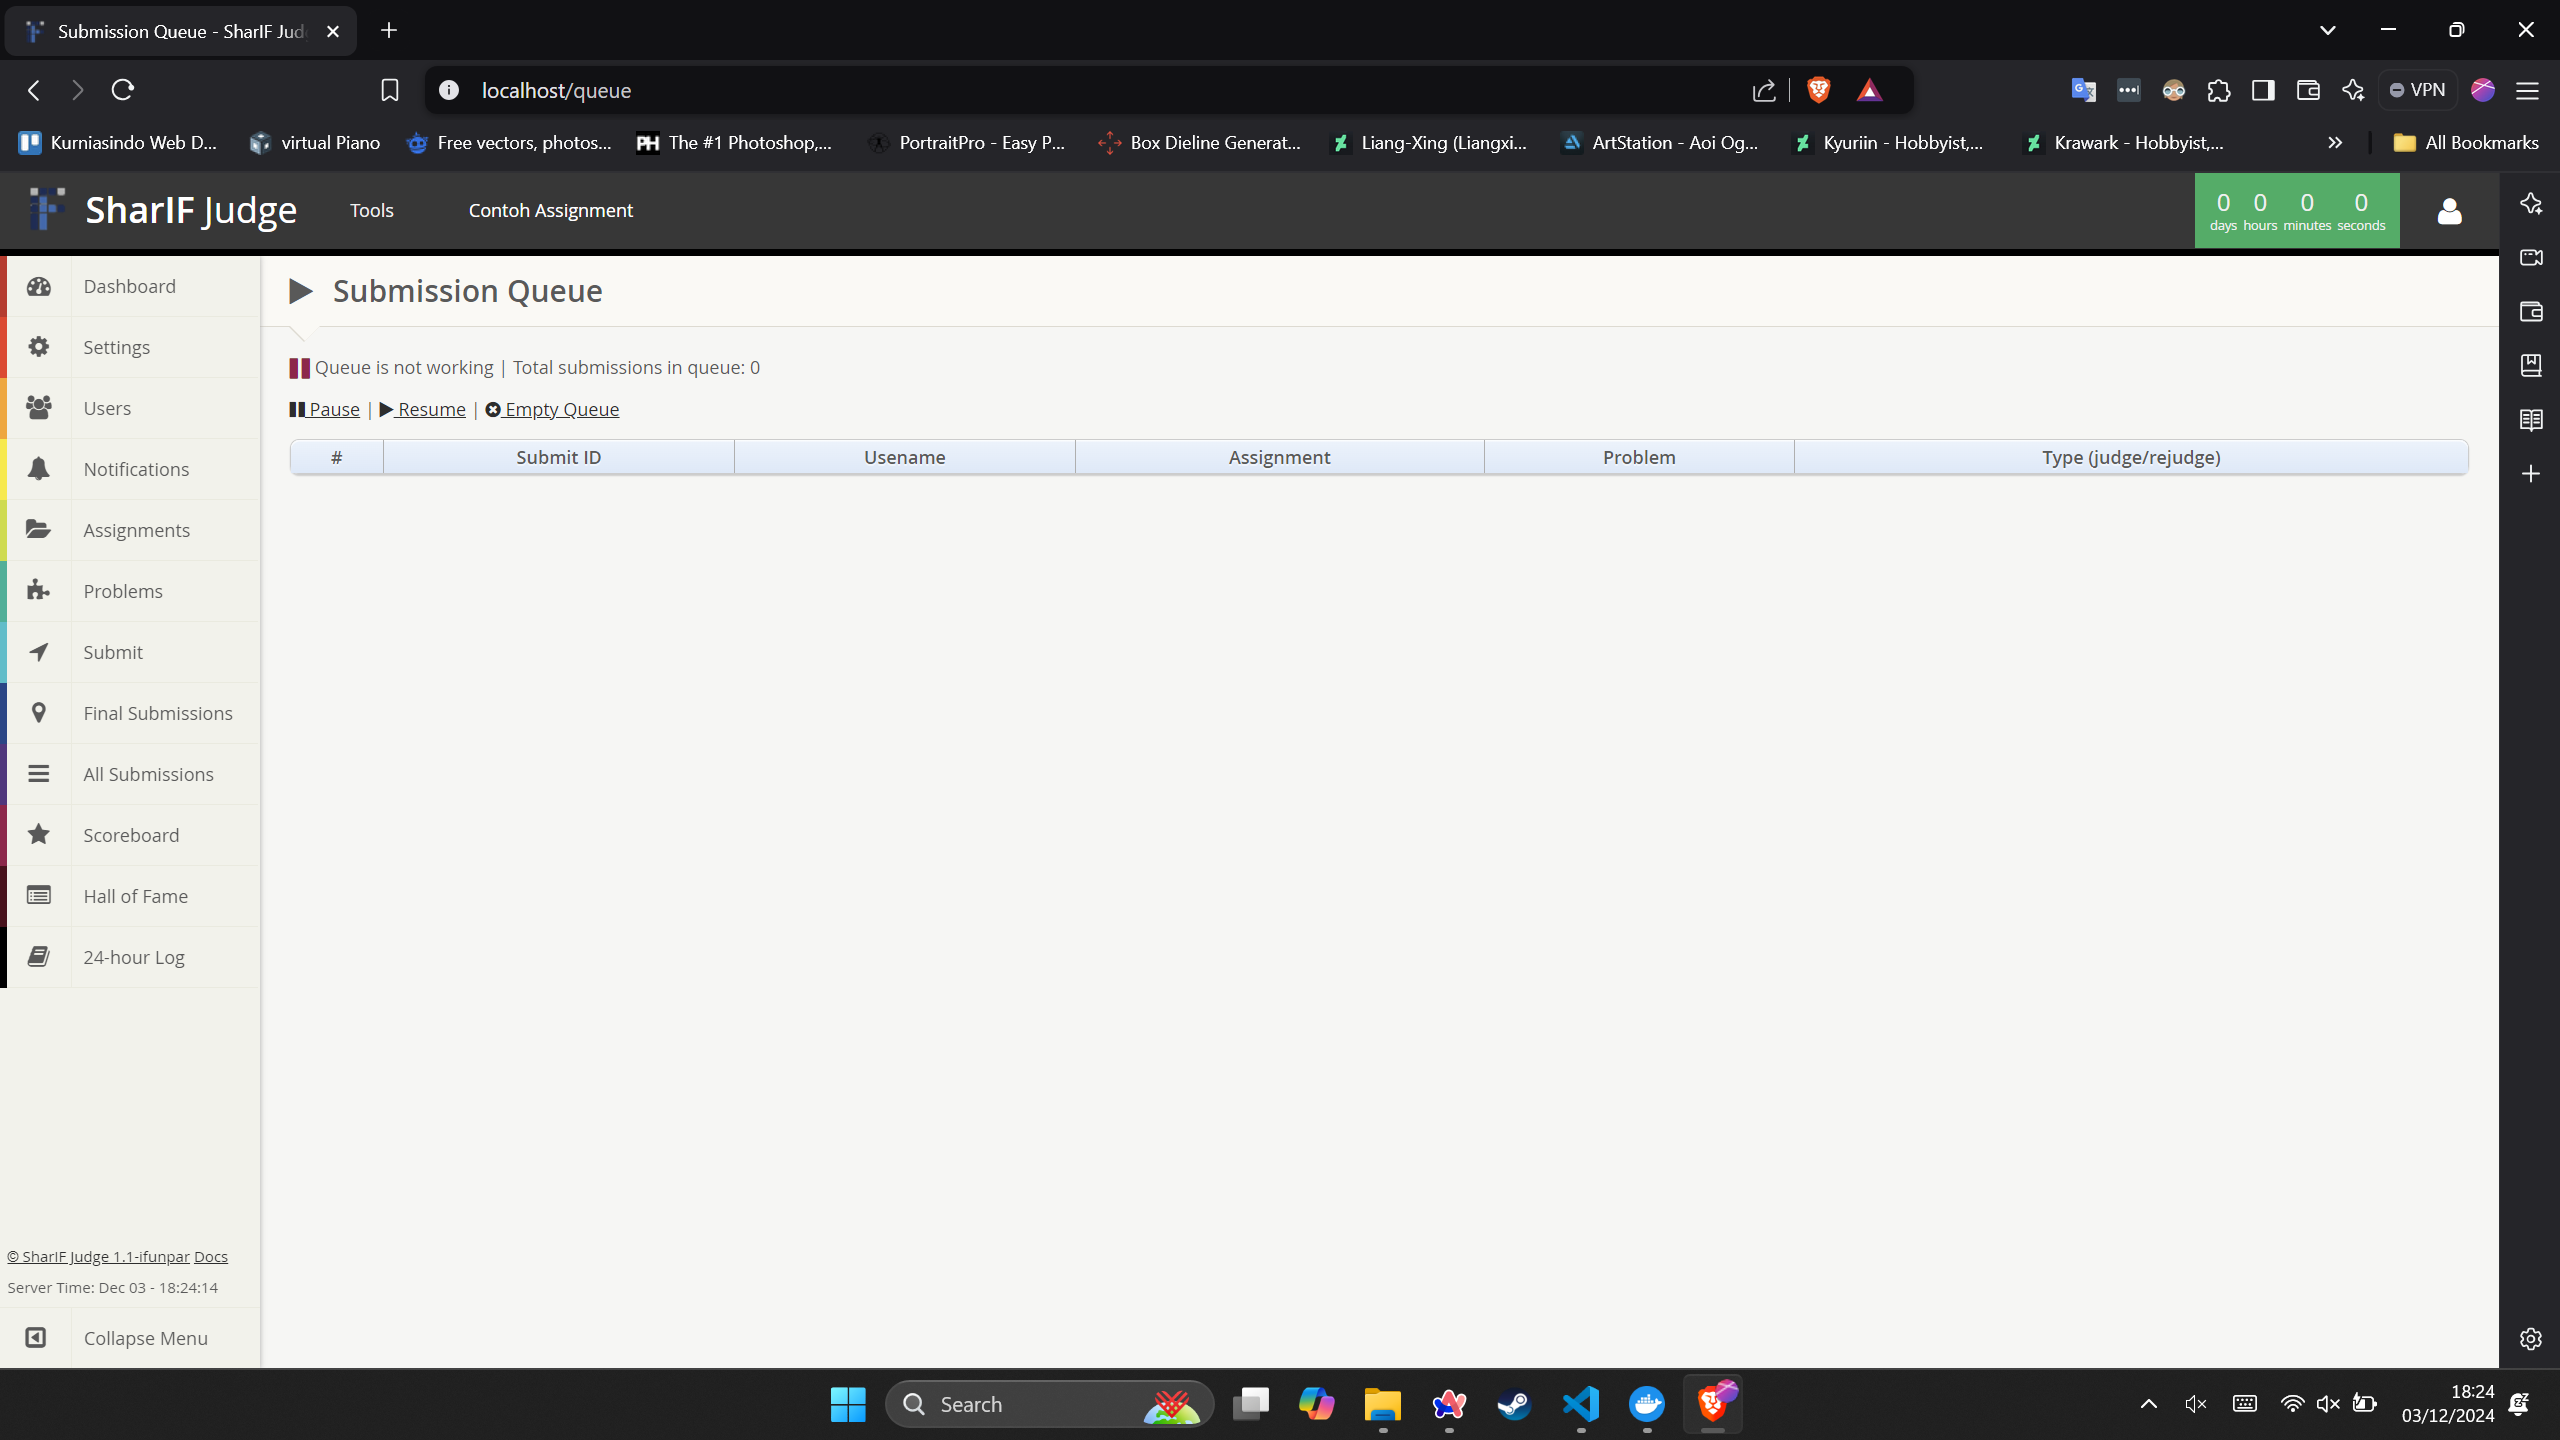
\includegraphics[width=\textwidth]{views/queue.png}
	      %       \caption{Halaman Queue}
	      %       \label{fig:3:1:1:queue}
	      % \end{figure}

	      % Gambar \ref{fig:3:1:1:queue} menunjukkan halaman Queue.
	\item Cheat Detection %controller
	      \begin{figure}[H]
		      \centering
		      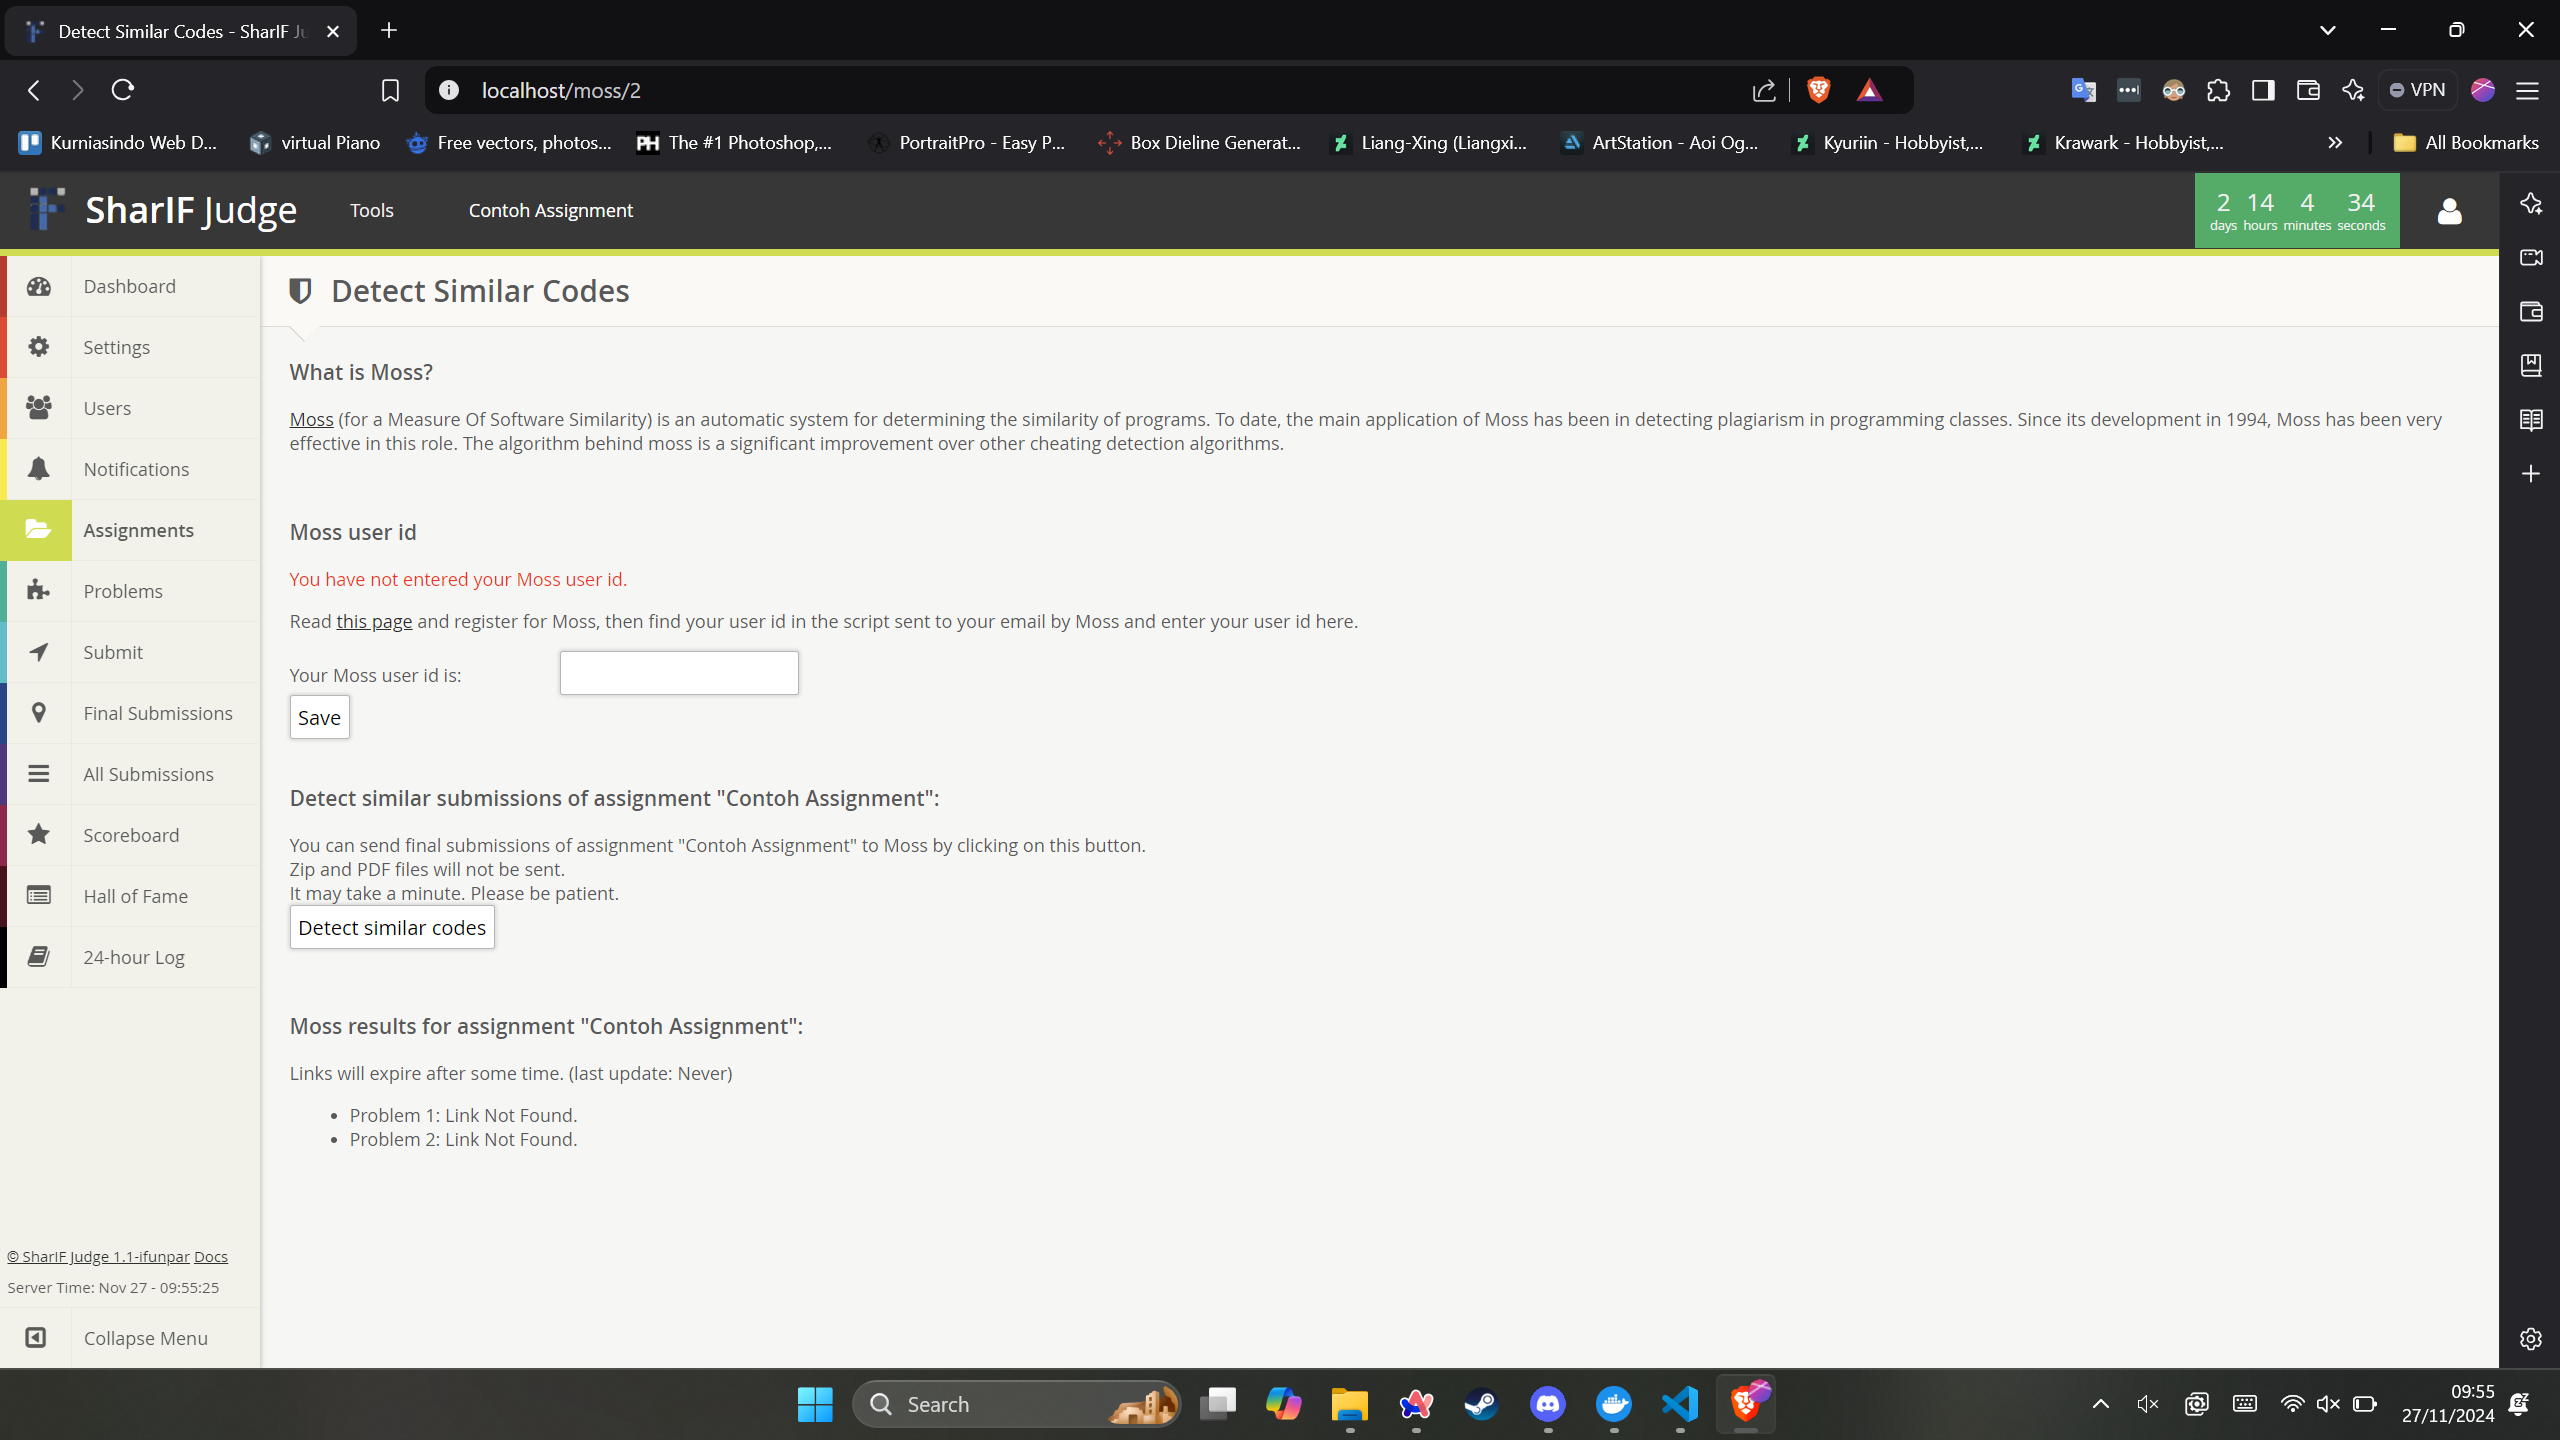
\includegraphics[width=\textwidth]{views/moss.png}
		      \caption{Halaman Cheat Detection}
		      \label{fig:3:1:1:moss}
	      \end{figure}

	      Gambar \ref{fig:3:1:1:moss} menunjukkan halaman Cheat Detection. Halaman ini hanya dapat di akses oleh \textit{role admin} dan \textit{head instructor}.

	\item Problems %controller
	      \begin{figure}[H]
		      \centering
		      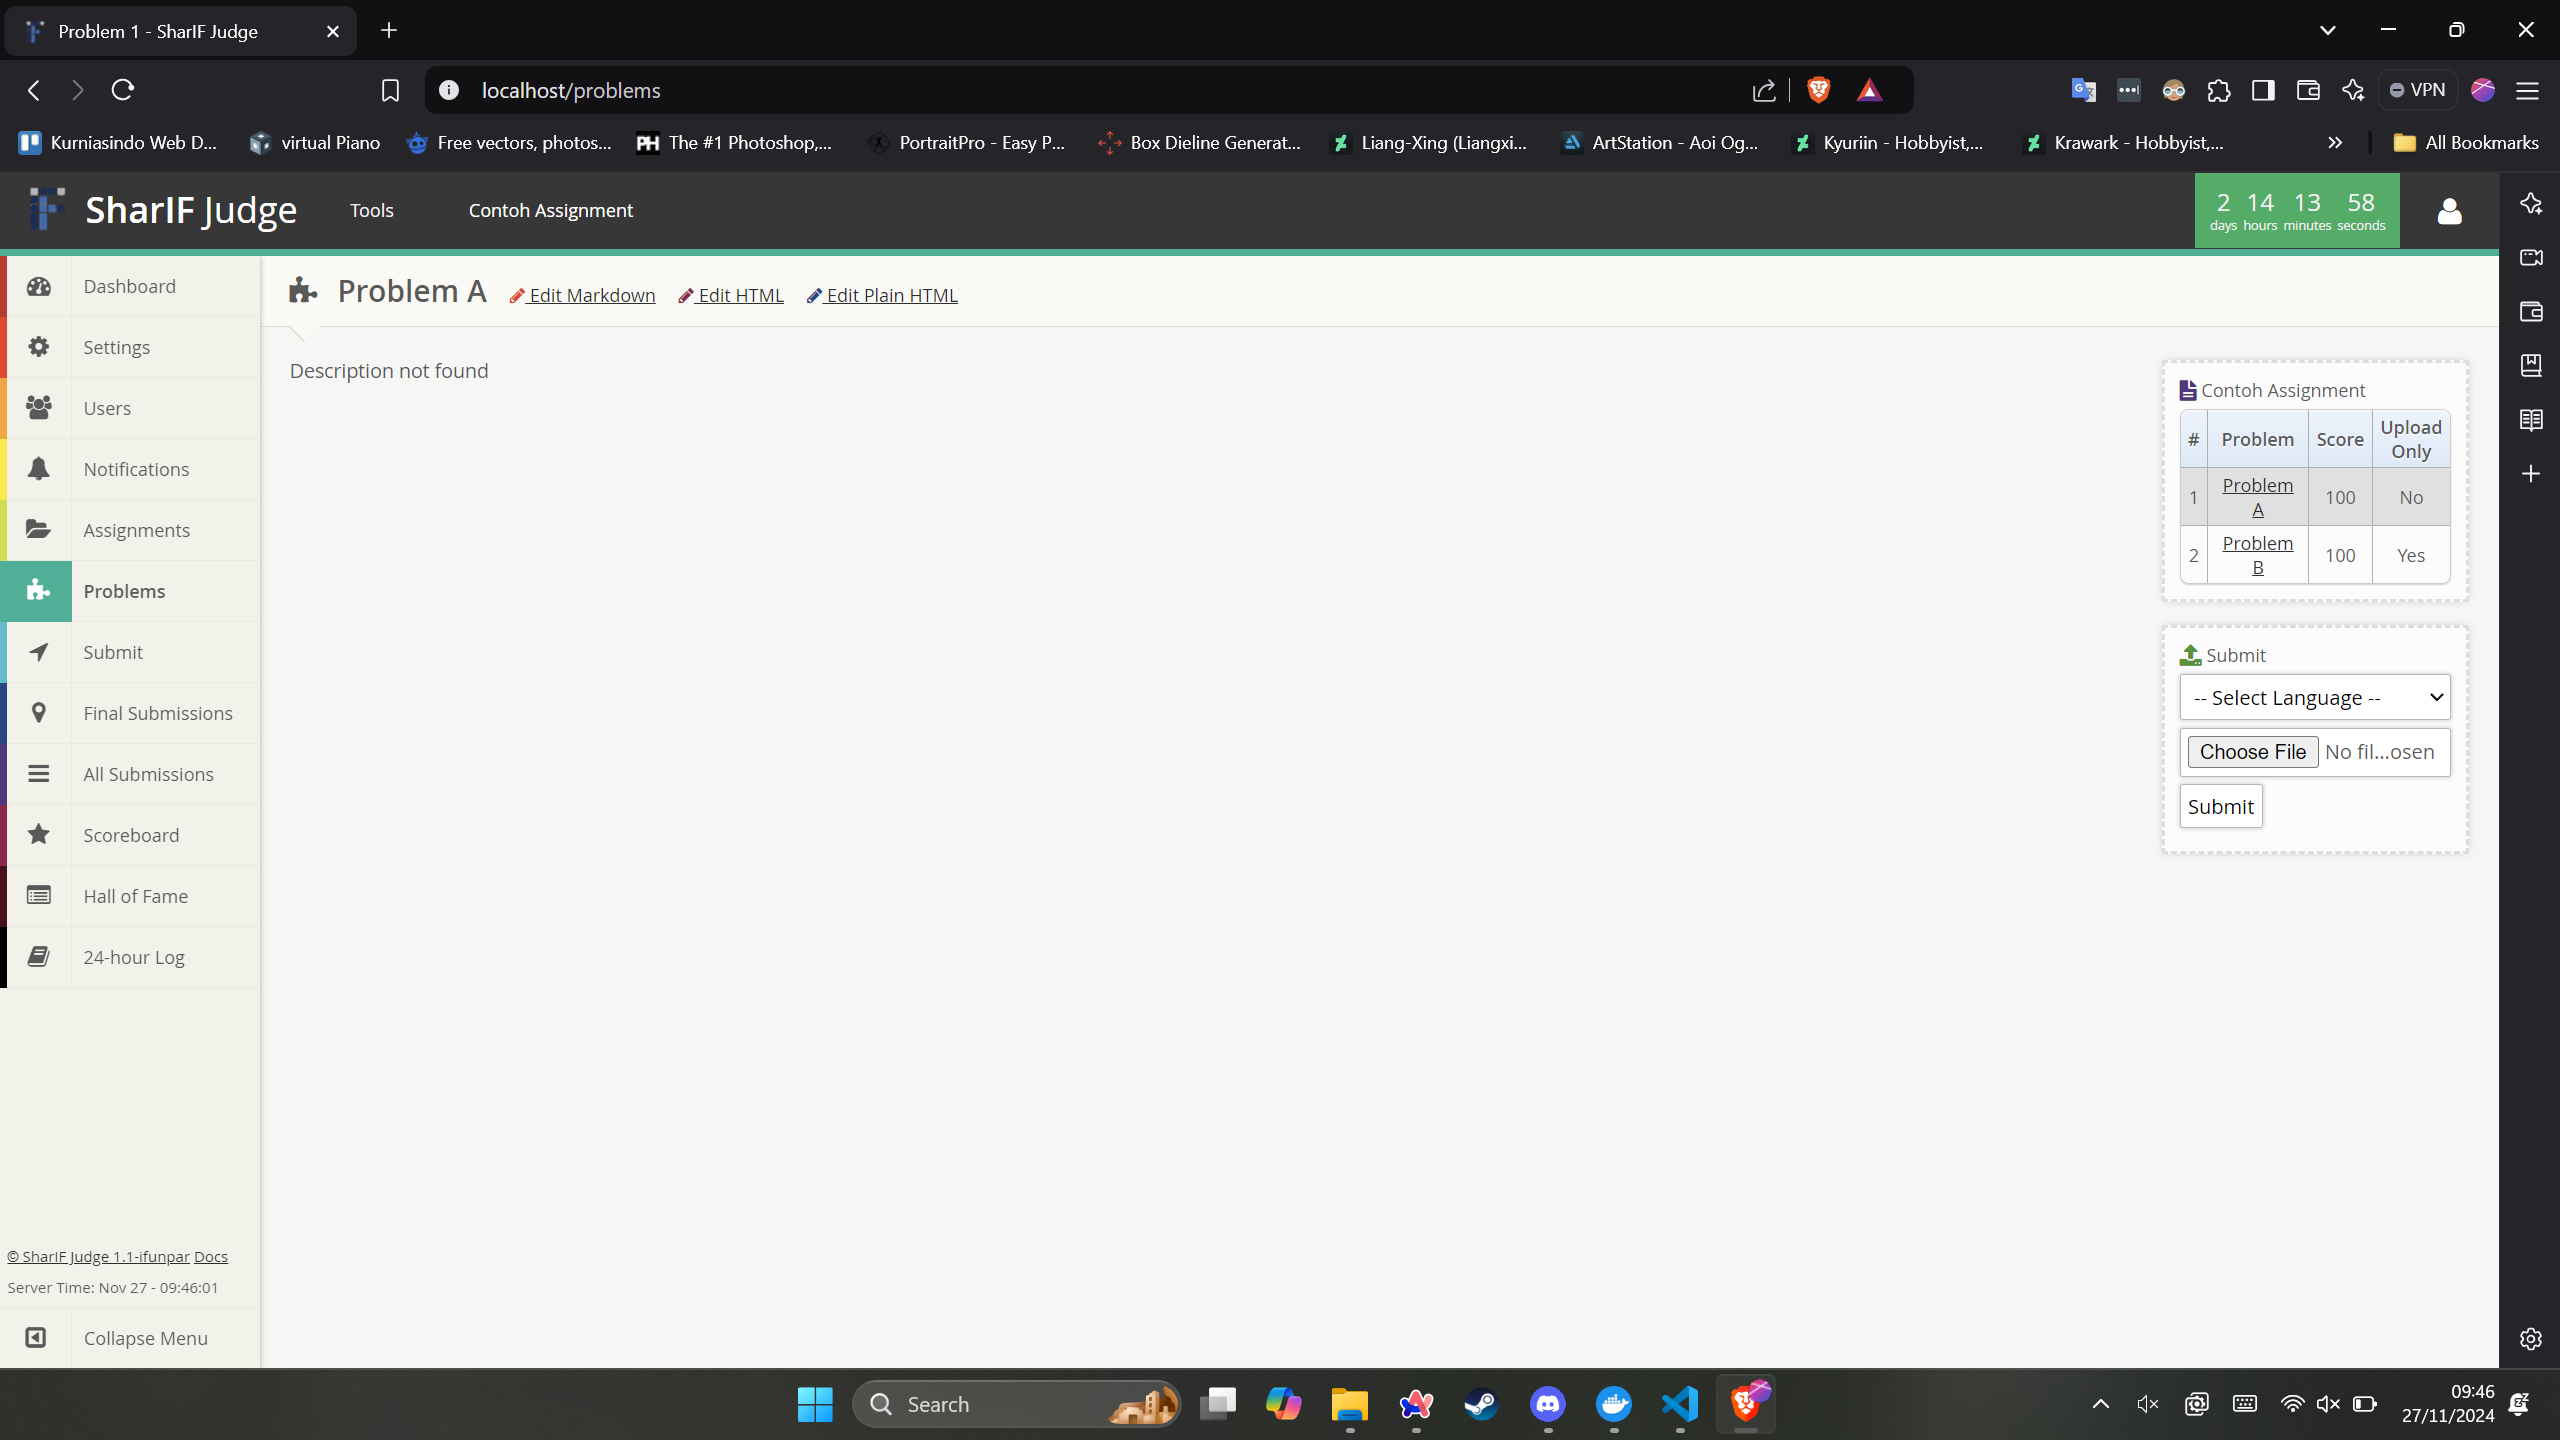
\includegraphics[width=\textwidth]{views/problem.png}
		      \caption{Halaman Problems}
		      \label{fig:3:1:1:problem}
	      \end{figure}

	      Gambar \ref{fig:3:1:1:problem} menunjukkan halaman Problems yang dapat diakses oleh semua \textit{role}.

	\item Submit %controller
	      \begin{figure}[H]
		      \centering
		      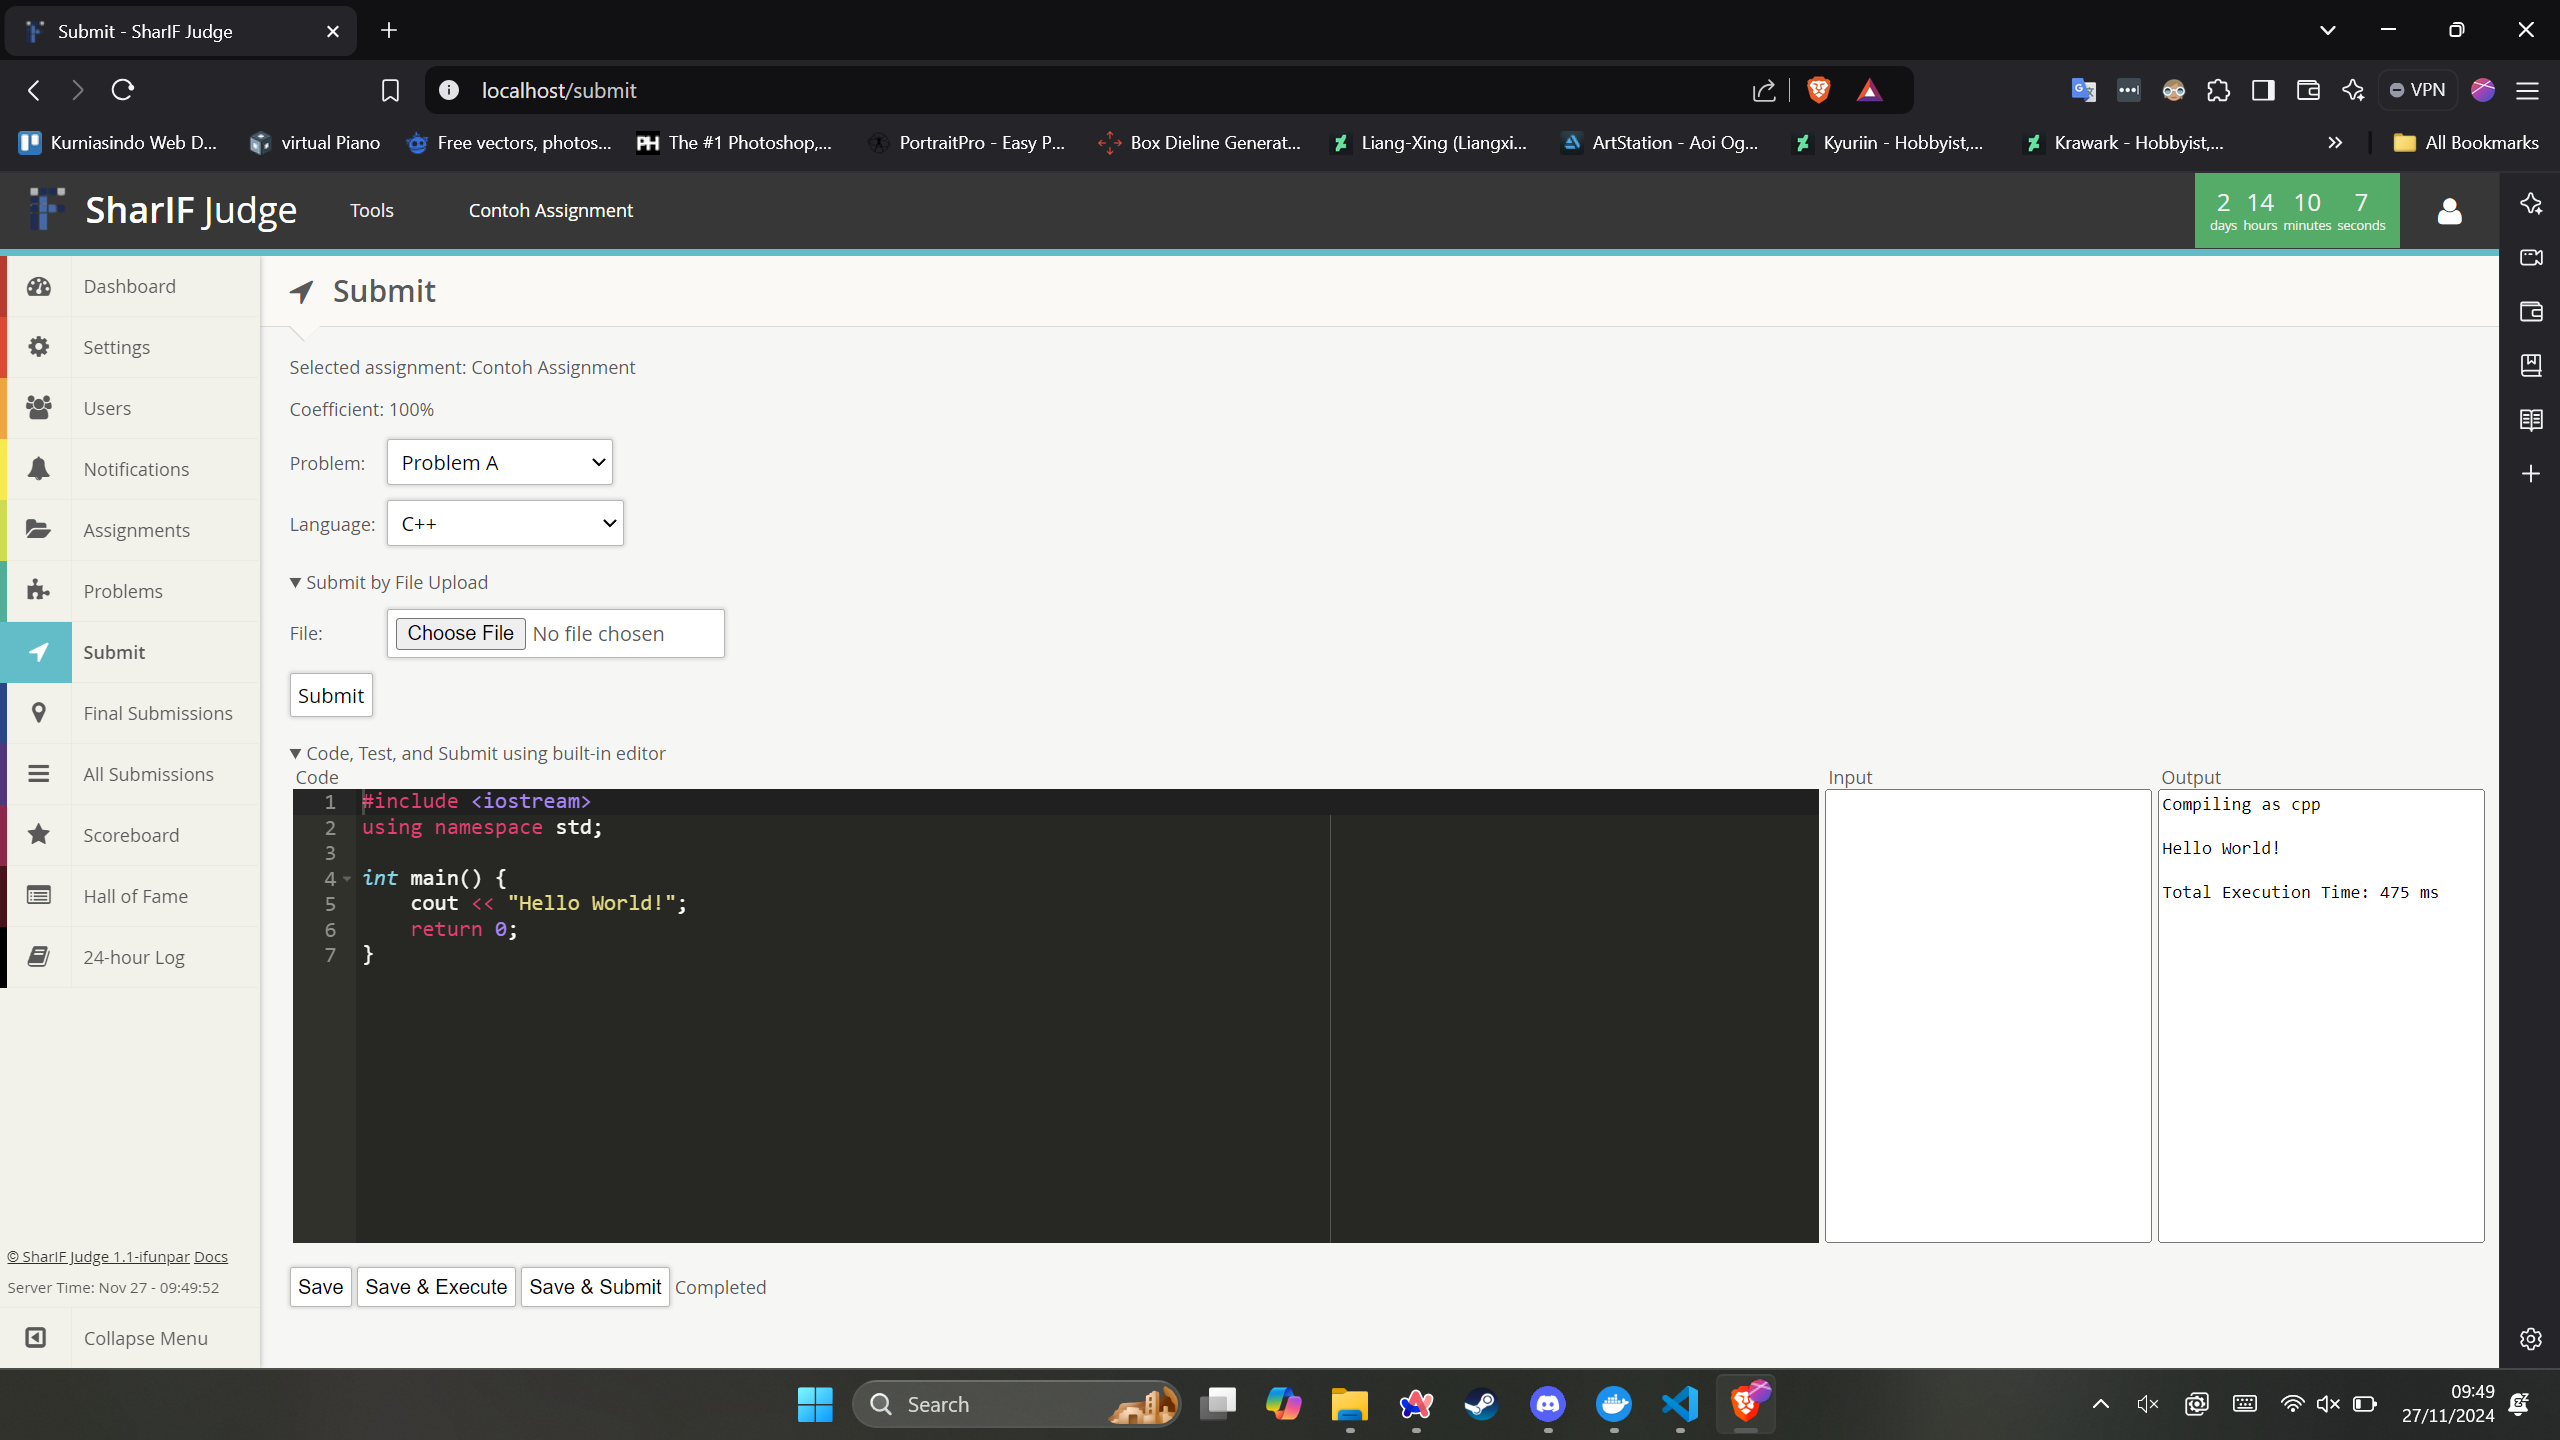
\includegraphics[width=\textwidth]{views/submit.png}
		      \caption{Halaman Submit}
		      \label{fig:3:1:1:submit}
	      \end{figure}

	      Gambar \ref{fig:3:1:1:submit} menunjukkan halaman Submit yang dapat diakses oleh semua \textit{role}. Halaman ini terdapat editor kode yang sudah di implementasikan~\cite{nicholas:sharif}.

	\item Final Submissions %controller
	      \begin{figure}[H]
		      \centering
		      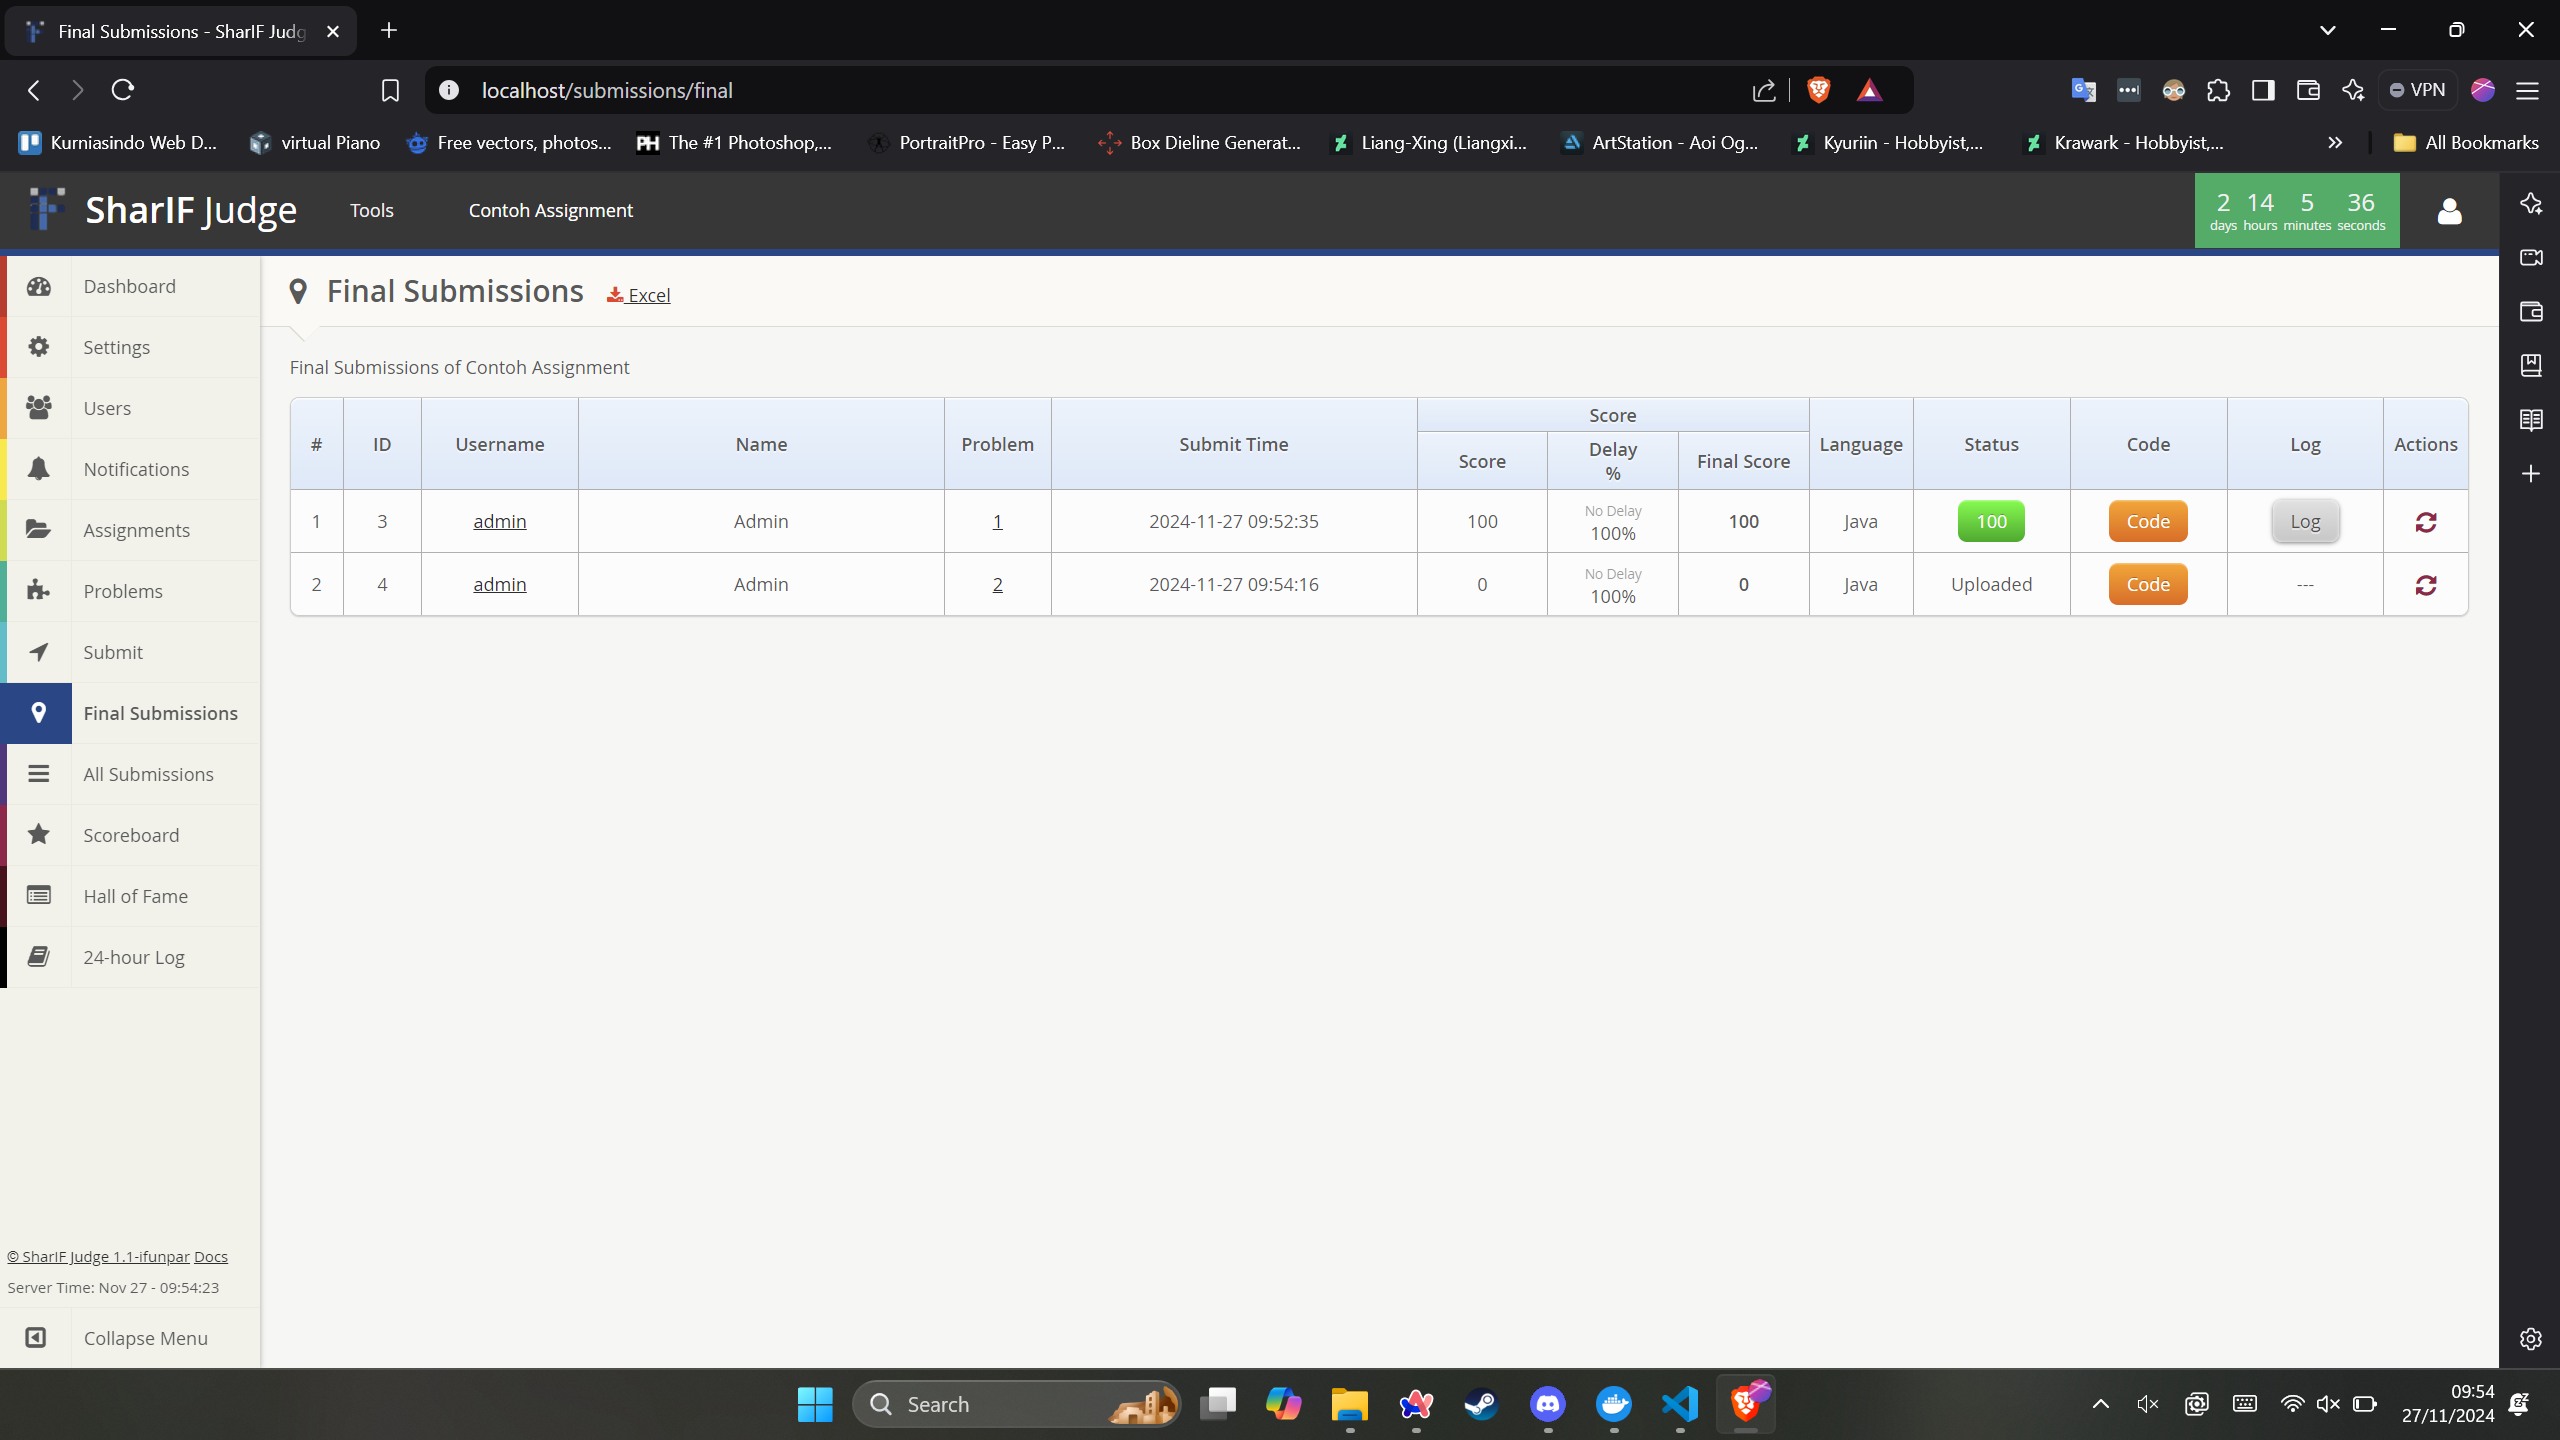
\includegraphics[width=\textwidth]{views/final_submissions.png}
		      \caption{Halaman Final Submissions}
		      \label{fig:3:1:1:final}
	      \end{figure}

	      Gambar \ref{fig:3:1:1:final} menunjukkan halaman Final Submissions yang dapat diakses oleh semua \textit{role}.

	\item All Submissions %controller
	      \begin{figure}[H]
		      \centering
		      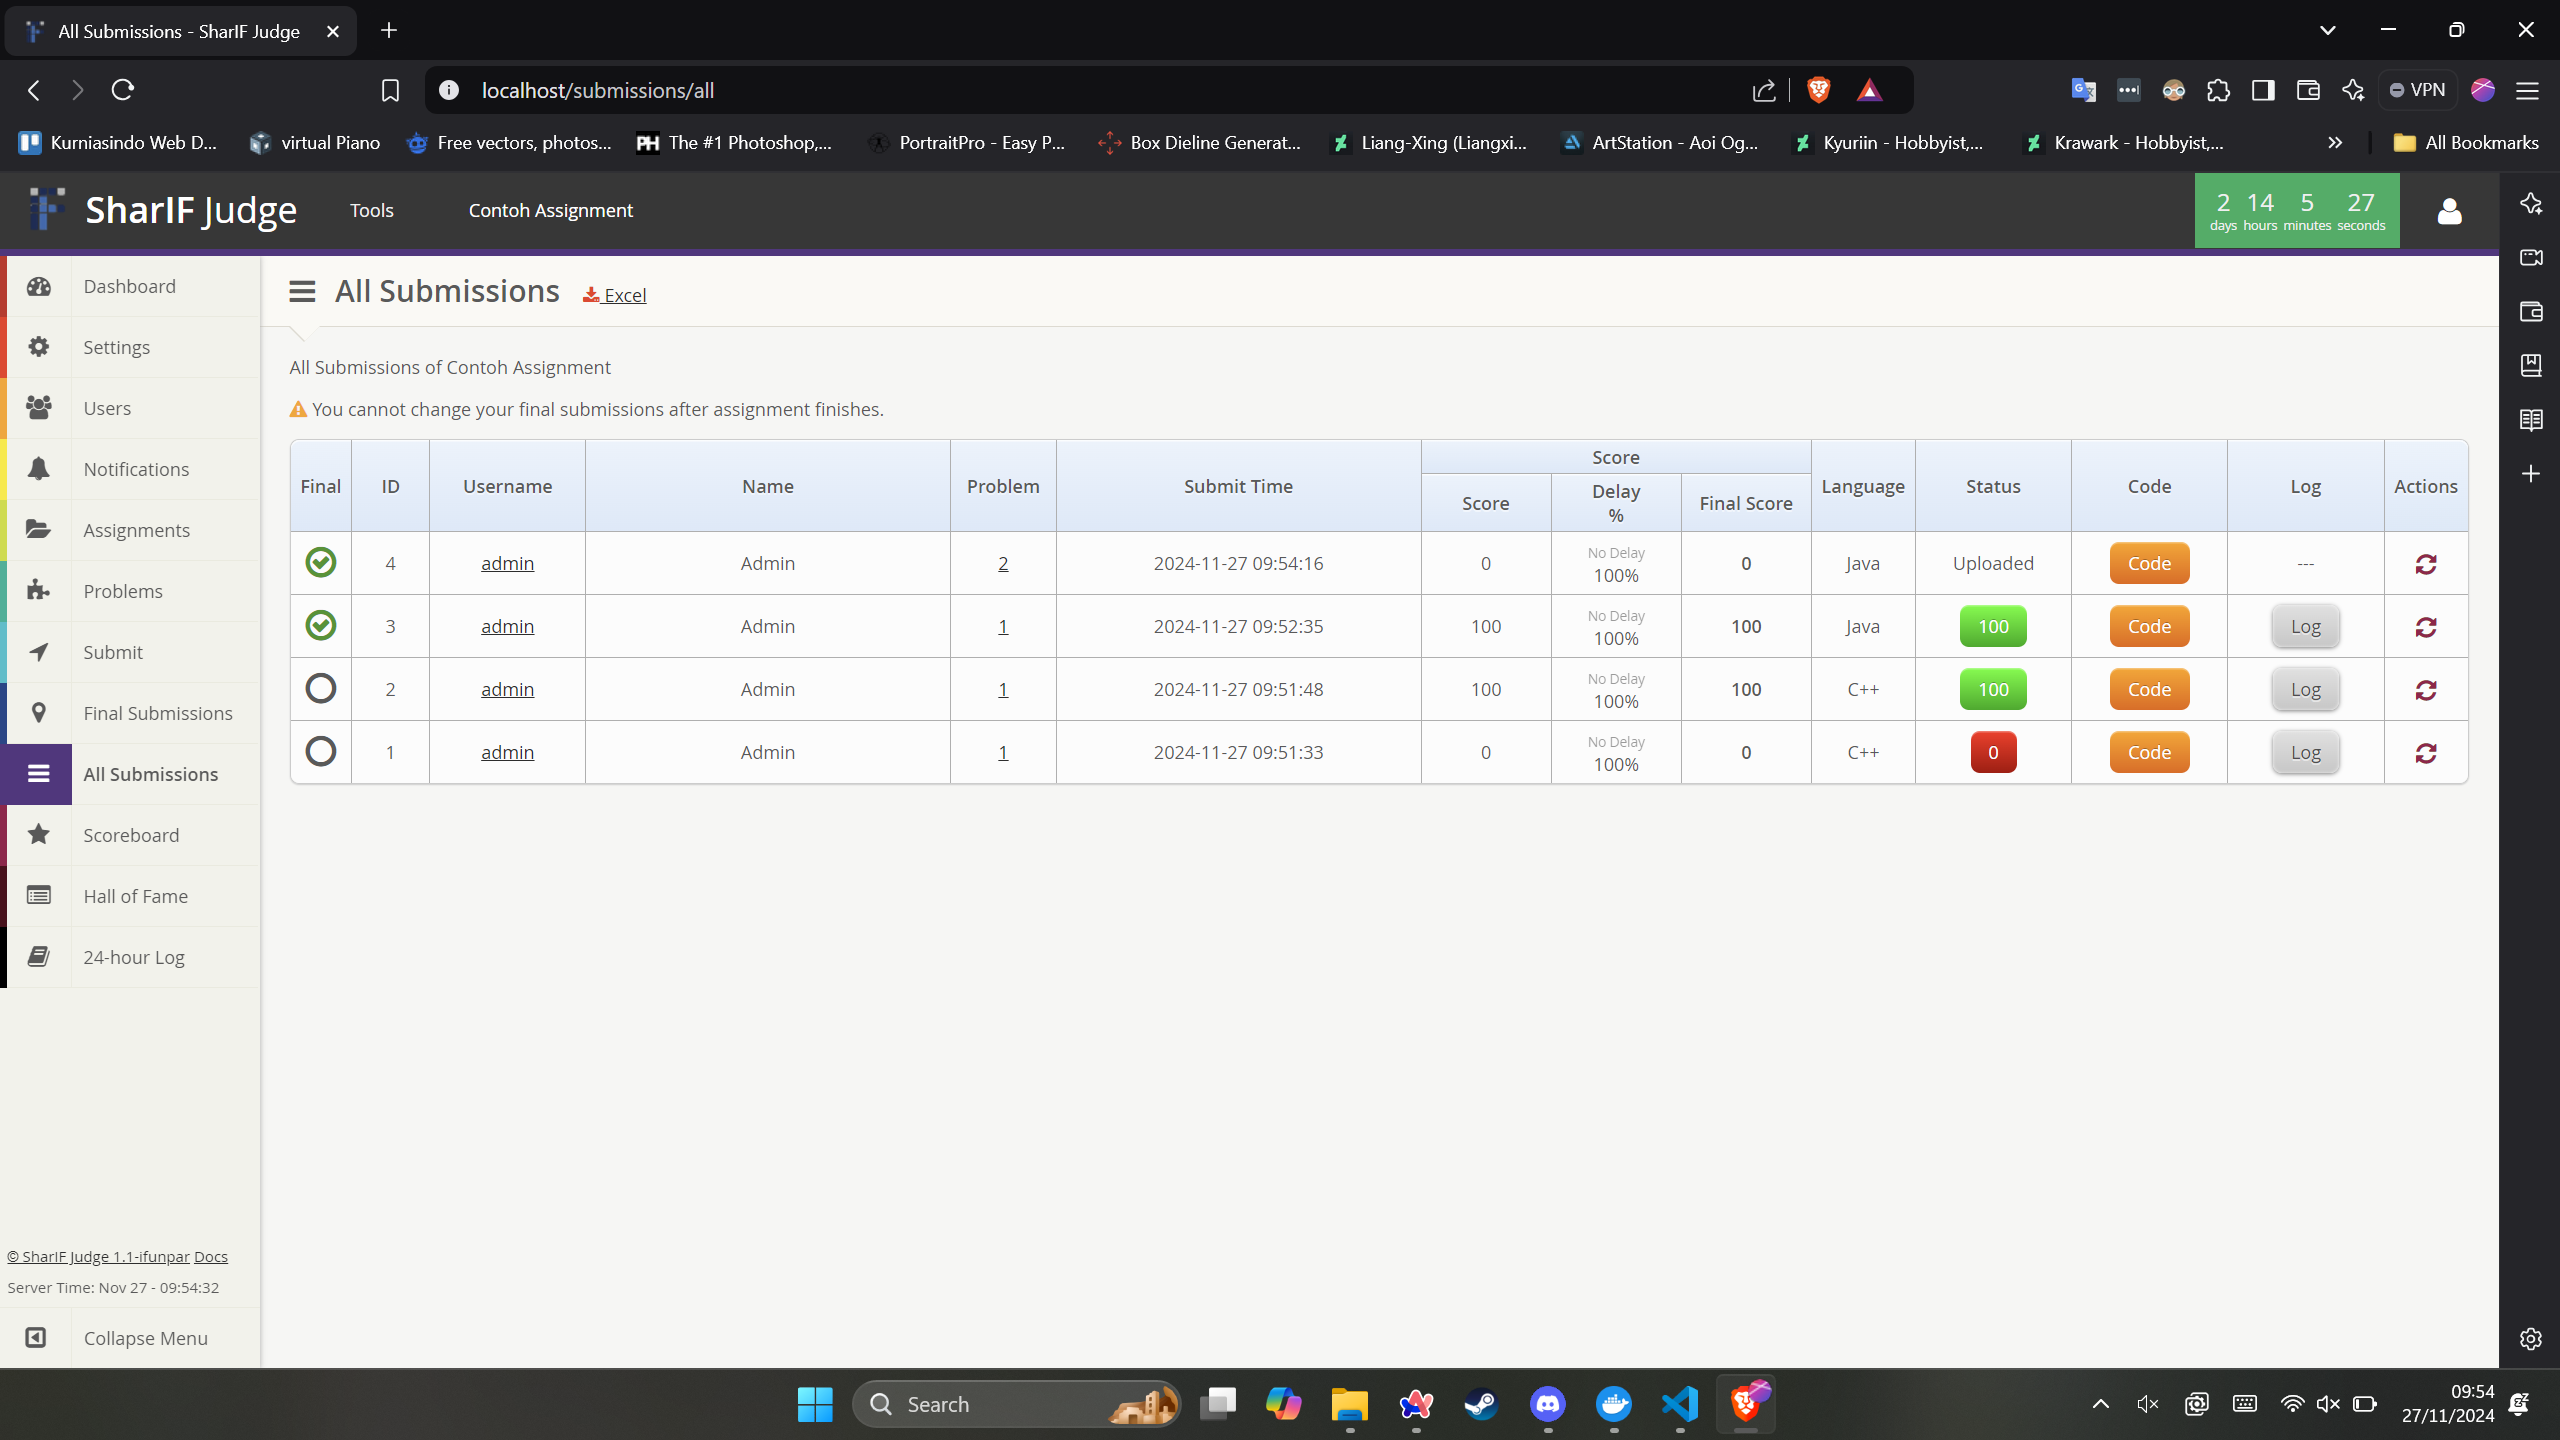
\includegraphics[width=\textwidth]{views/all_submissions.png}
		      \caption{Halaman All Submissions}
		      \label{fig:3:1:1:all}
	      \end{figure}

	      Gambar \ref{fig:3:1:1:all} menunjukkan halaman All Submissions yang dapat diakses oleh semua \textit{role}.
	\item Scoreboard %controller
	      \begin{figure}[H]
		      \centering
		      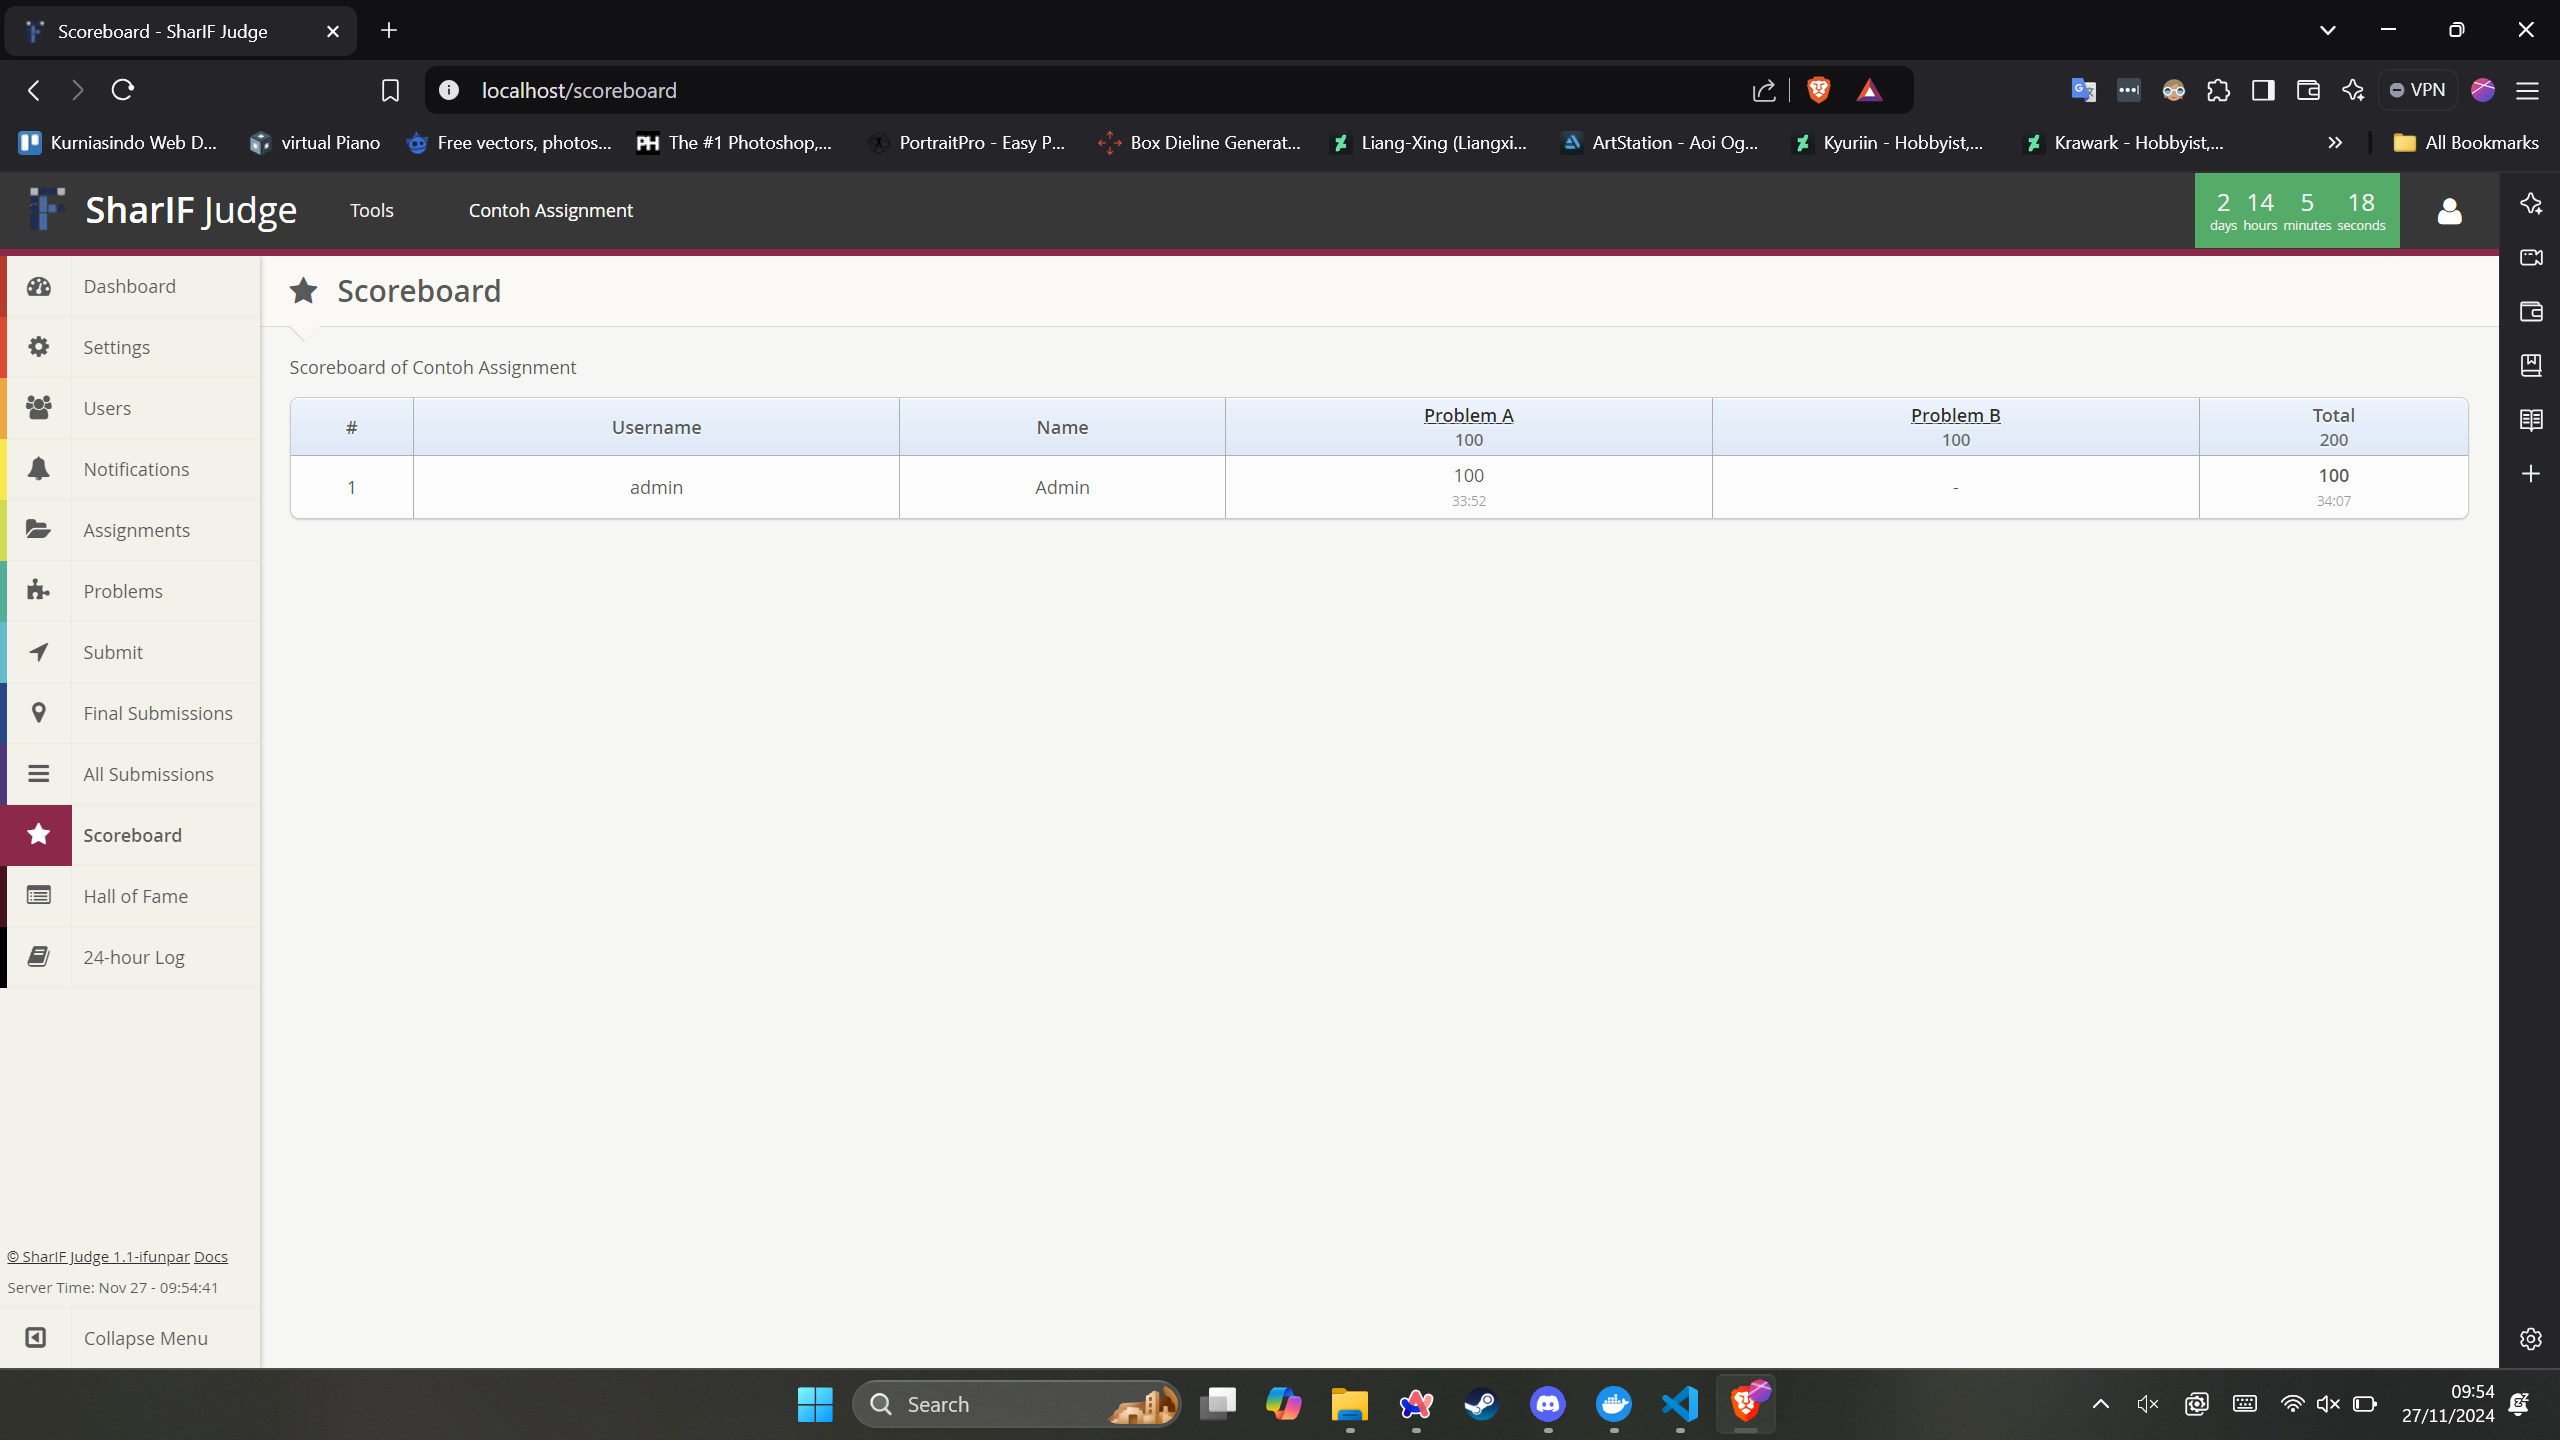
\includegraphics[width=\textwidth]{views/scoreboard.png}
		      \caption{Halaman Scoreboard}
		      \label{fig:3:1:1:scoreboard}
	      \end{figure}

	      Gambar \ref{fig:3:1:1:scoreboard} menunjukkan halaman Scoreboard yang dapat diakses oleh semua \textit{role}.

	\item Hall of Fame %controller
	      \begin{figure}[H]
		      \centering
		      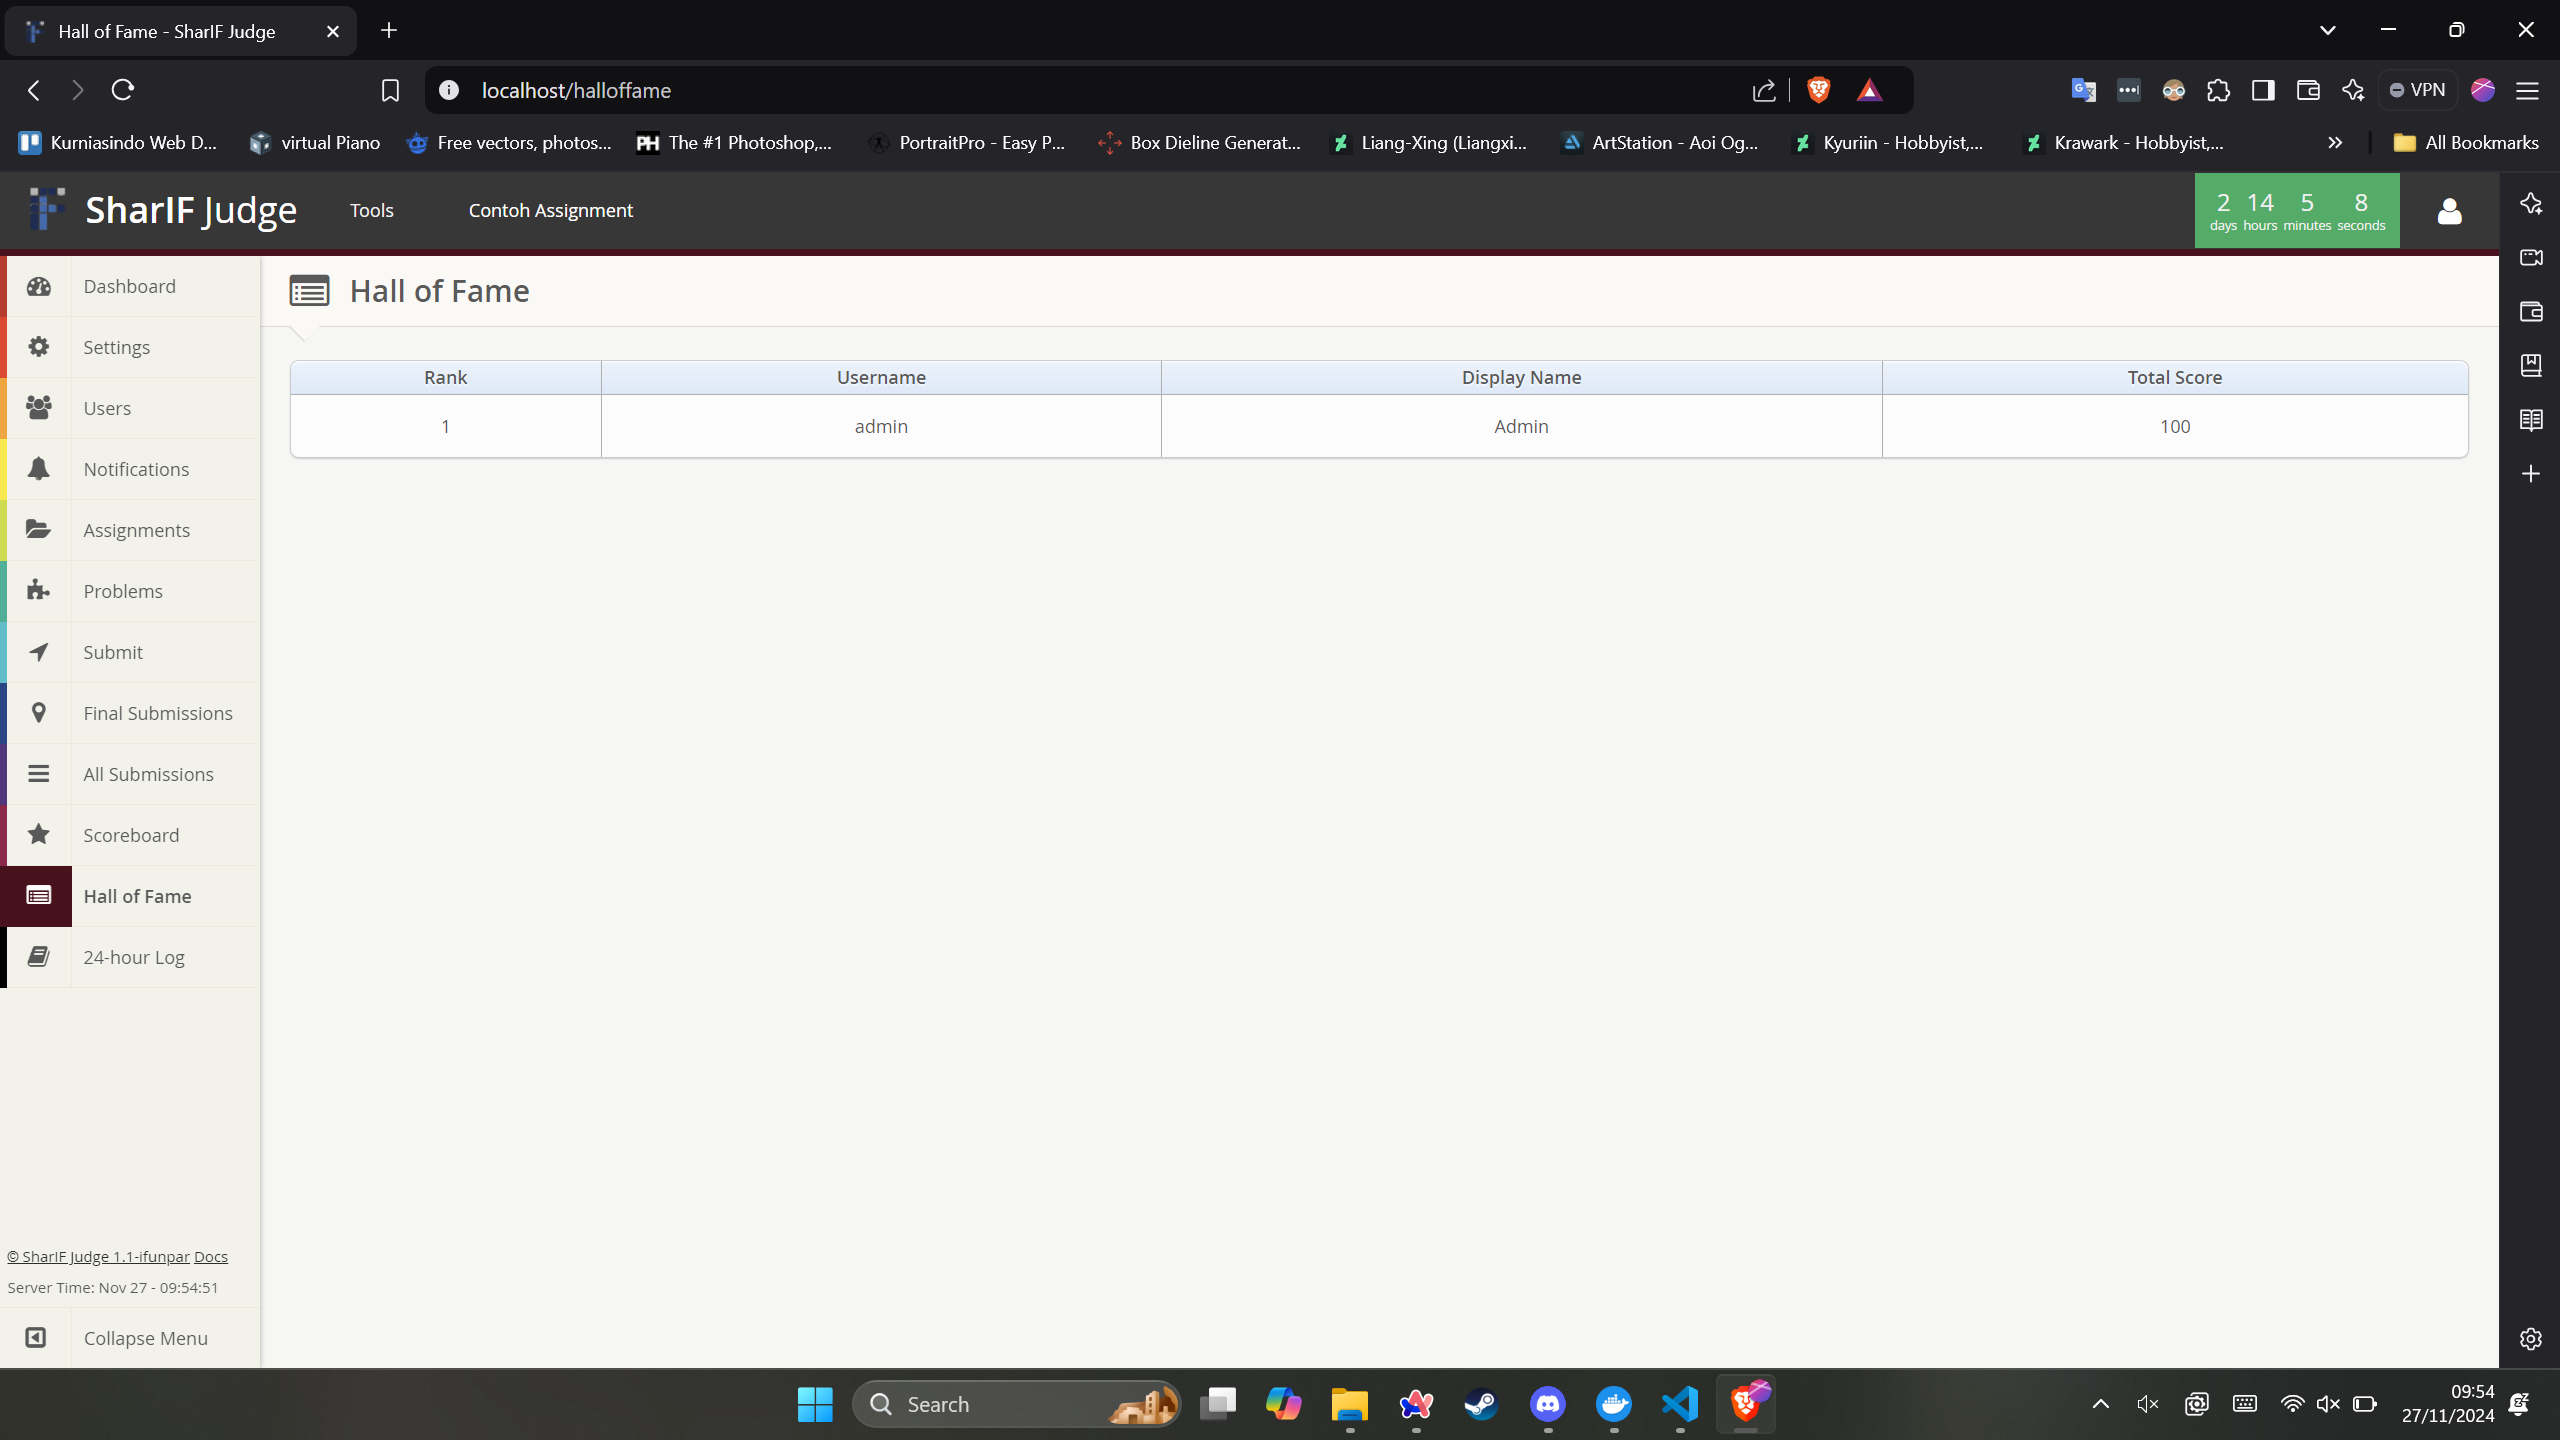
\includegraphics[width=\textwidth]{views/hof.png}
		      \caption{Halaman Hall of Fame}
		      \label{fig:3:1:1:hof}
	      \end{figure}

	      Gambar \ref{fig:3:1:1:hof} menunjukkan halaman Hall of Fame yang dapat diakses oleh semua \textit{role}.

	\item 24-Hour Log %controller
	      \begin{figure}[H]
		      \centering
		      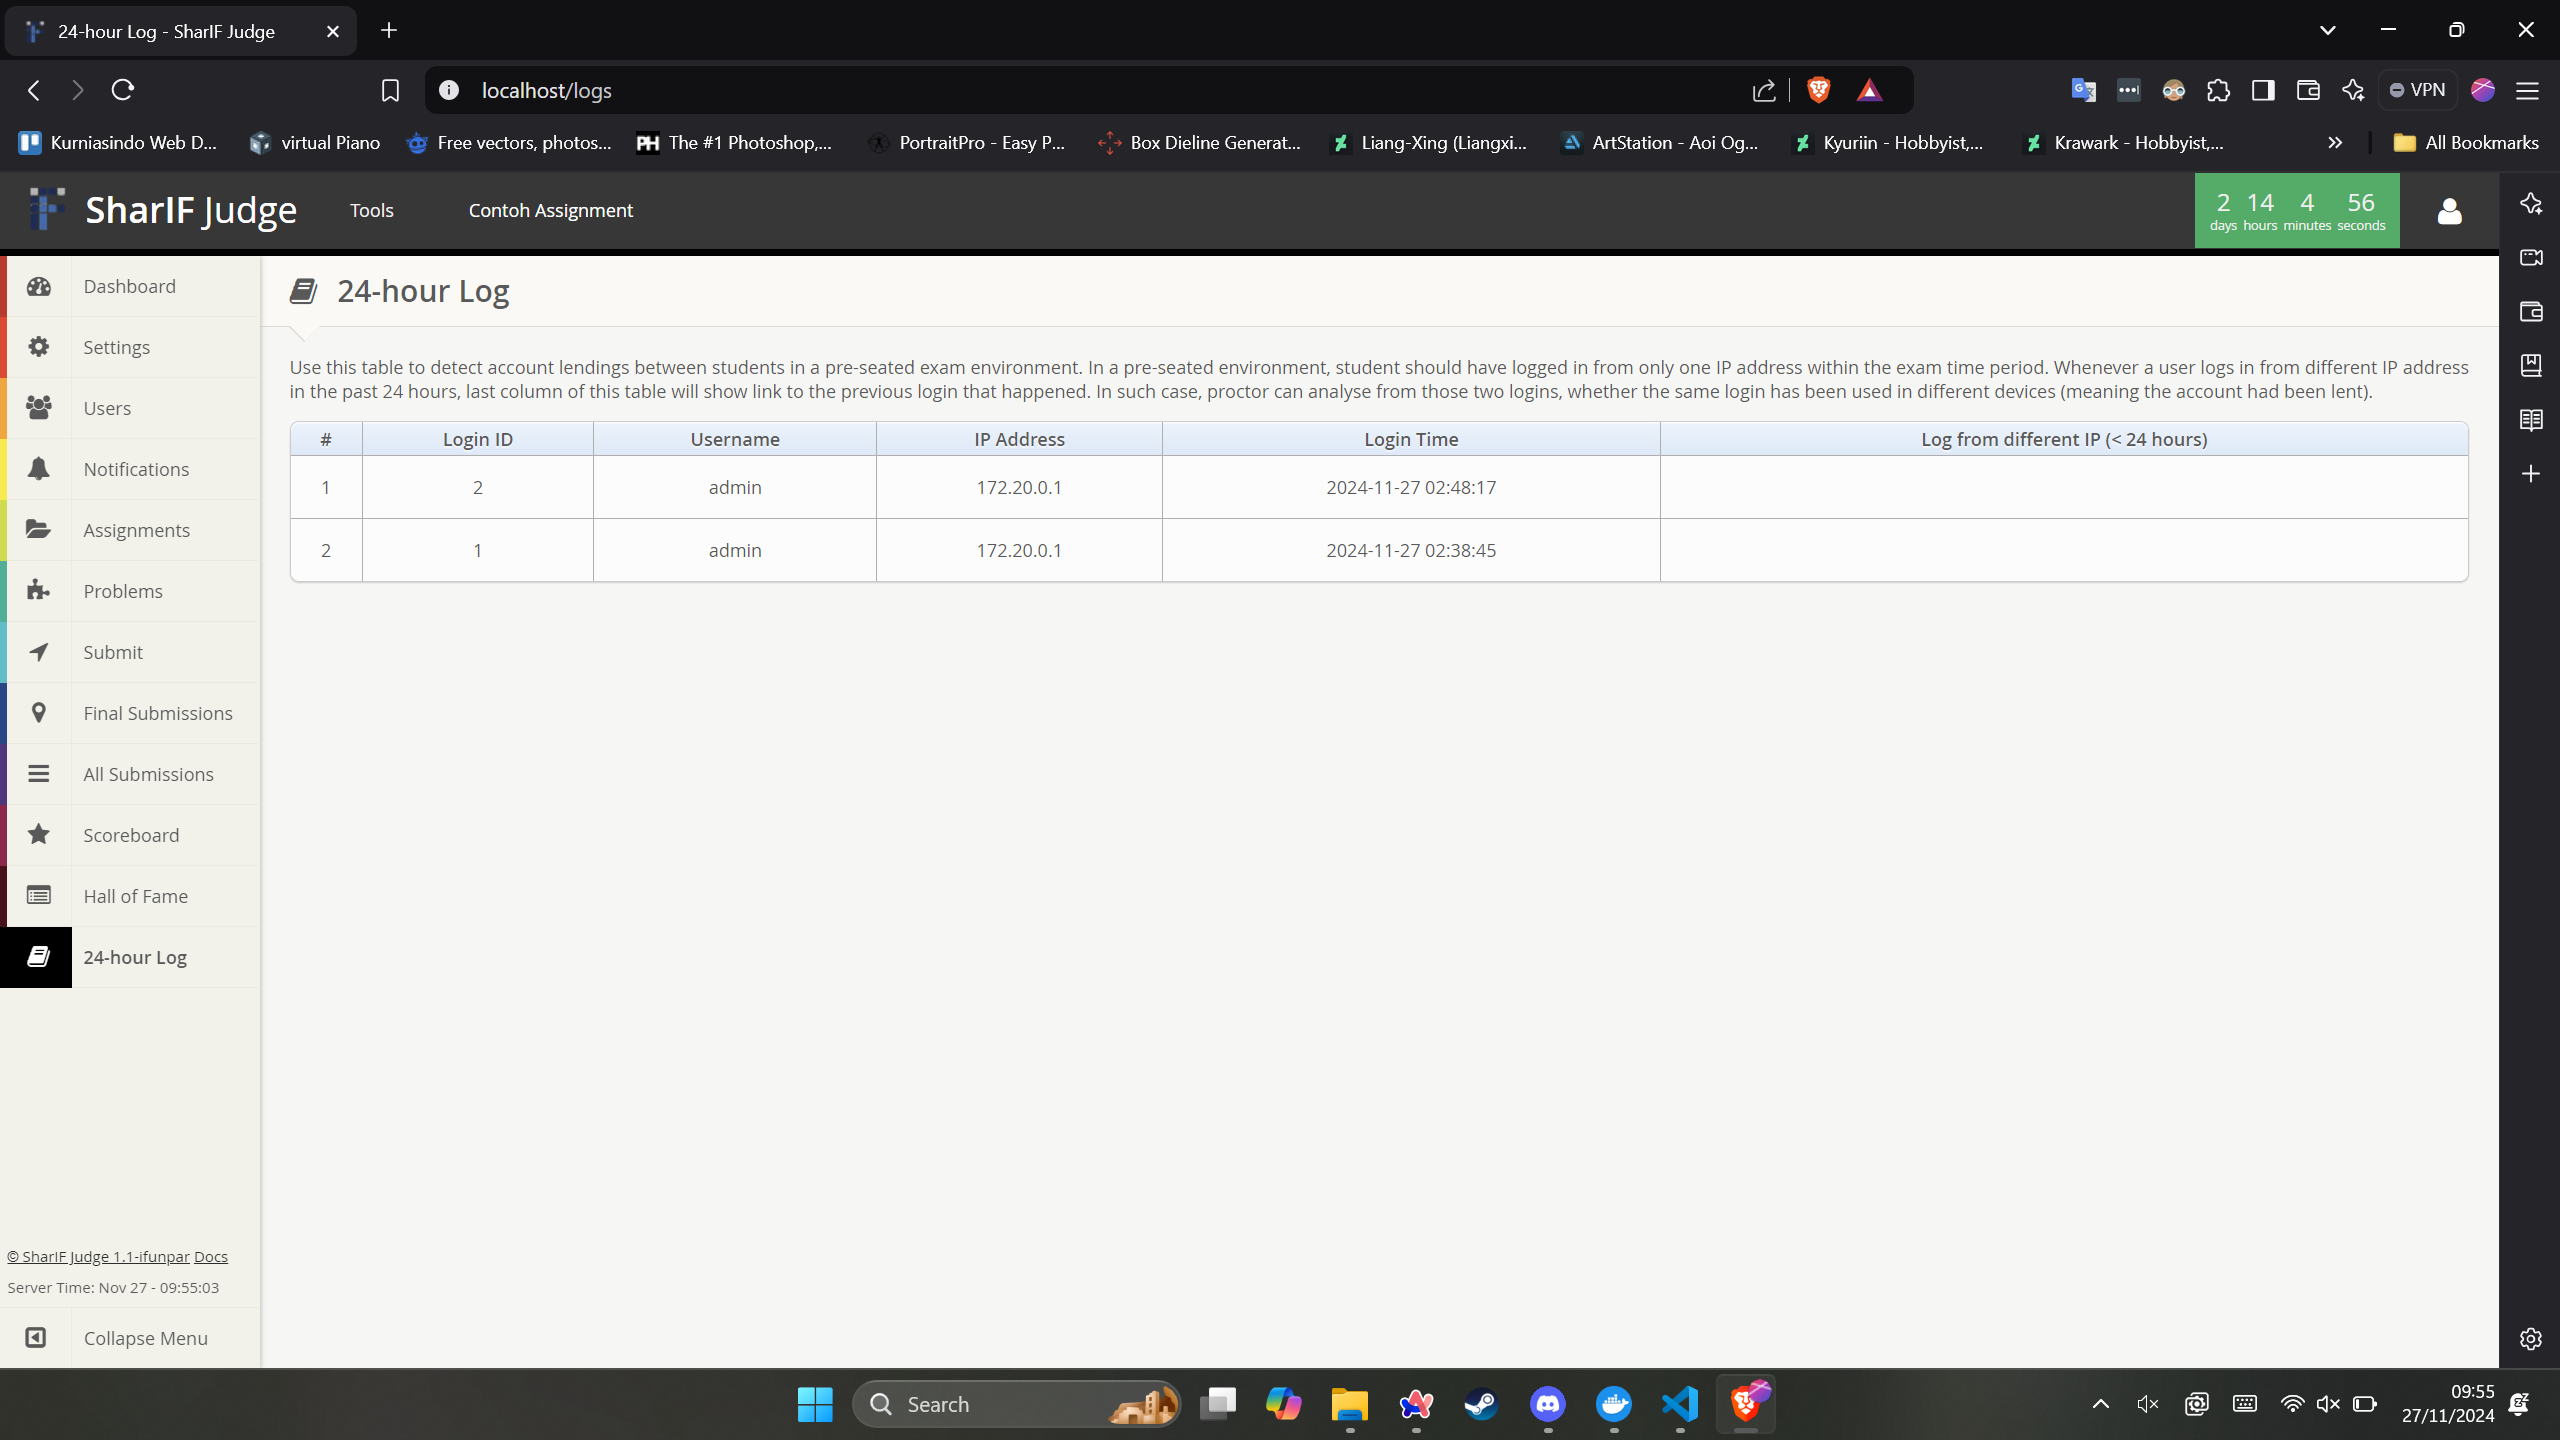
\includegraphics[width=\textwidth]{views/log.png}
		      \caption{Halaman 24-Hour Log}
		      \label{fig:3:1:1:log}
	      \end{figure}

	      Gambar \ref{fig:3:1:1:log} menunjukkan halaman 24-Hour Log. Halaman ini hanya dapat di akses oleh \textit{role admin} dan \textit{head instructor}.

\end{itemize}
\end{comment}

\subsubsection{Controller}
\label{sub:3:1:1:controller}

Pada bagian analisis MVC terakhir, terdapat \textit{controller} yang berada pada direktori \\ \verb|application/controller|. Seperti yang dijelaskan pada bab \ref{sub:2:2:3:Controller}, \textit{Controller} digunakan sebagai perantara antara \textit{model}, \textit{view}, dan \textit{resources} lainnya yang dibutuhkan saat membuat sebuah web page. Direktori controller berisi kelas-kelas yang akan mengolah data yang didapat pada \textit{model} dan menyatukan data tersebut ke dalam \textit{views} yang akan ditampilkan kepada pengguna. Pada setiap kelas \textit{controller}, terdapat fungsi \verb|index()| yang menjadi fungsi utama saat kelas di akses oleh pengguna. Berikut merupakan file \textit{controller} dan penjelasan fungsi-fungsinya yang terdapat pada SharIF Judge:

\begin{itemize}
	\item \verb|Assignments.php| \\
	      Berikut fungsi dengan penjelasannya pada \textit{controller} \verb|Assignments.php|:

	      \begin{itemize}
		      \item \verb|select()| \\
		            Memilih \textit{assignment} yang ditampilkan pada \textit{top bar} menggunakan \textit{ajax request}.
		      \item \verb|pdf($assignment_id, $problem_id, $no_download)| \\
		            Mengunduh \textit{assignment} atau \textit{problem} dalam bentuk \textit{pdf file} ke browser.
		      \item \verb|downloadtestsdesc($assignment_id)| \\
		            Mengunduh dan mencompress data uji dan deskripsi sebuah \textit{assignment}.
		      \item \verb|download_submissions($type, $assignment_id)| \\
		            Mengunduh semua \textit{final submission} pada semua \textit{assignment}.
		      \item \verb|delete($assignment_id)| \\
		            Menghapus sebuah \textit{assignment}.
		      \item \verb|add()| \\
		            Mendapatkan \textit{input} dari pengguna untuk menambah atau memperbaharui sebuah \textit{assignment}.
		      \item \verb|_add()| \\
		            Menambahkan atau memperbaharui sebuah \textit{assignment}.
		      \item \verb|edit($assignment_id)| \\
		            Menandai \textit{assignment} yang akan di \textit{edit} dan memanggil fungsi \verb|add|.
		      \item \verb|pdfCheck($assignment_id, $problem_id)| \\
		            Melakukan validasi ketersediaan pdf pada sebuah \textit{assignment} atau pada sebuah \textit{problem}.
		      \item \verb|index()| \\
		            Mengambil data dari \verb|Assignment_model| dan menaruh data dan mengembalikan \textit{views} \verb|assignments.twig|. Gambar \ref{fig:3:1:1:assignments} menunjukkan hasil halaman Assignment.

		            \begin{figure}[H]
			            \centering
			            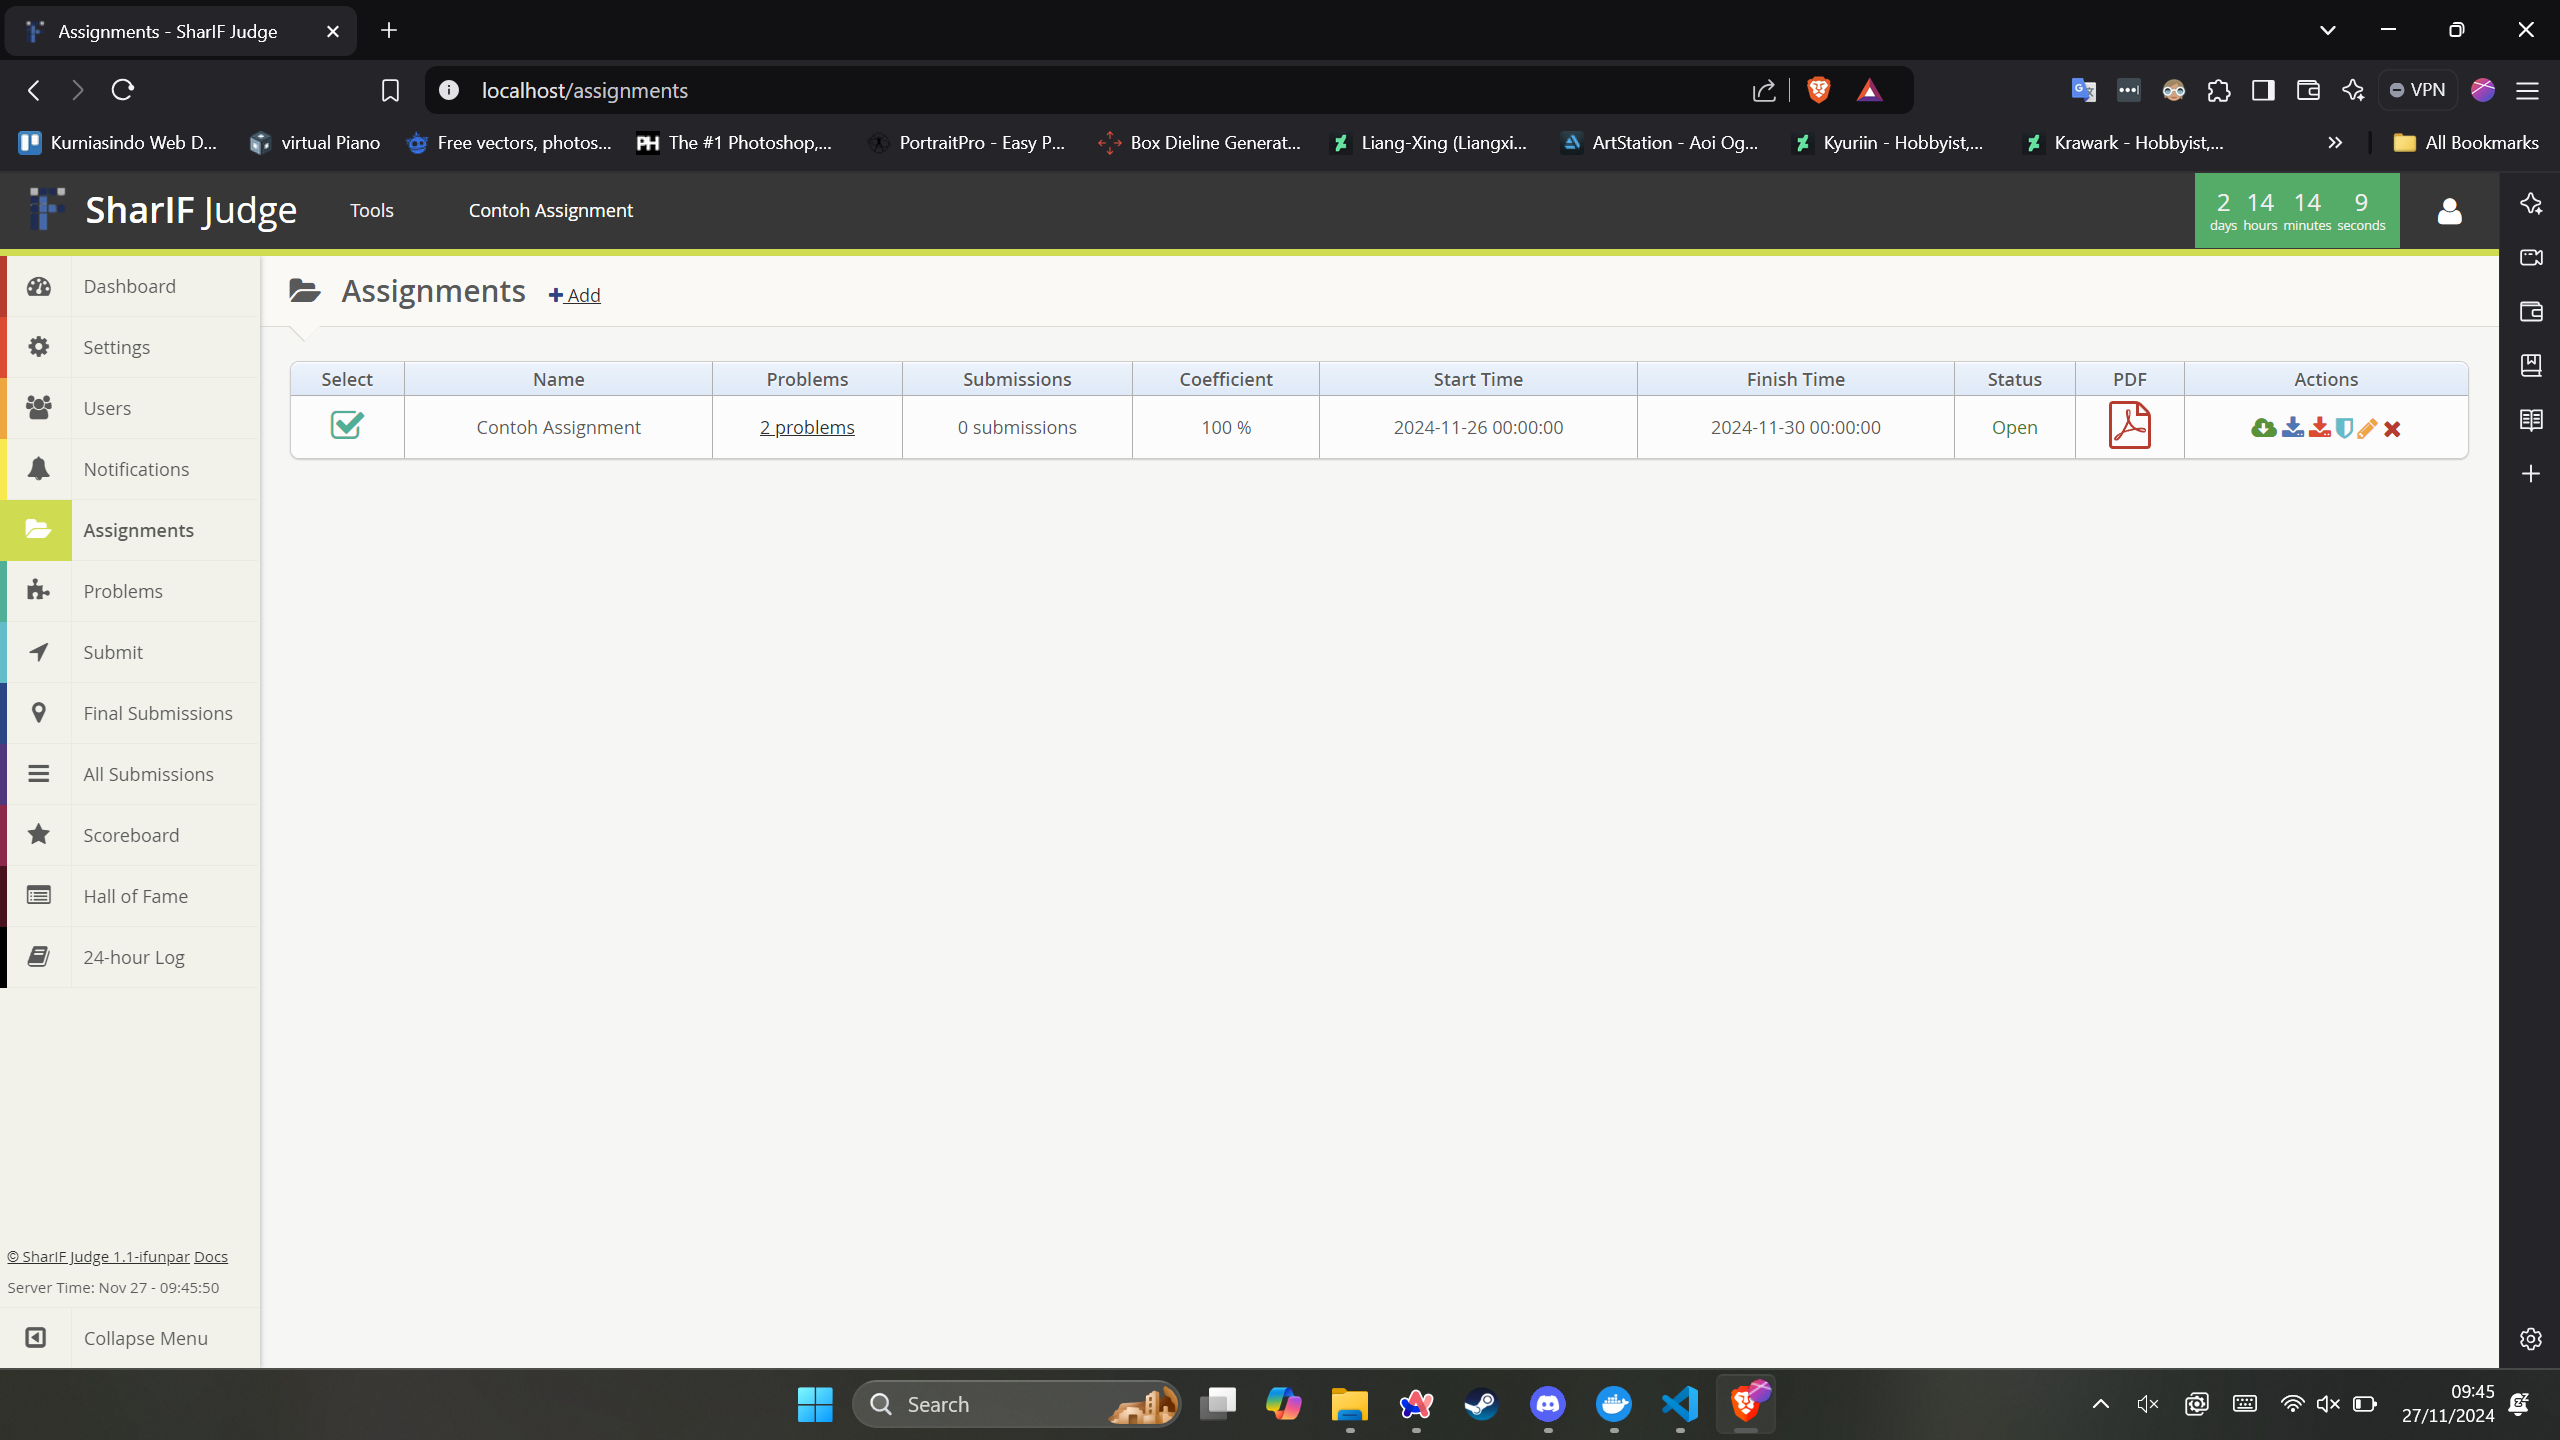
\includegraphics[width=\textwidth]{views/assignments.png}
			            \caption{Halaman Assignments}
			            \label{fig:3:1:1:assignments}
		            \end{figure}
	      \end{itemize}

	\item \verb|Dashboard.php| \\
	      Berikut fungsi dengan penjelasannya pada \textit{controller} \verb|Dashboard.php|:

	      \begin{itemize}
		      \item \verb|widget_positions()| \\
		            Mengunakan \textit{ajax request} untuk menyimpan posisi \textit{widget}.

		      \item \verb|index()| \\
		            Mendapatkan data dari beberapa model yaitu \verb|Assignment_model|, \verb|Settings_model|, \verb|User|, dan \verb|Notifications_model|. Data akan dimasukkan ke dalam \verb|dashboard.twig| yang akan dikembalikan ke pengguna. Gambar \ref{fig:3:1:1:dashboard} menunjukkan hasil halaman Dashboard yang dapat diakses oleh semua \textit{role}.

		            \begin{figure}[H]
			            \centering
			            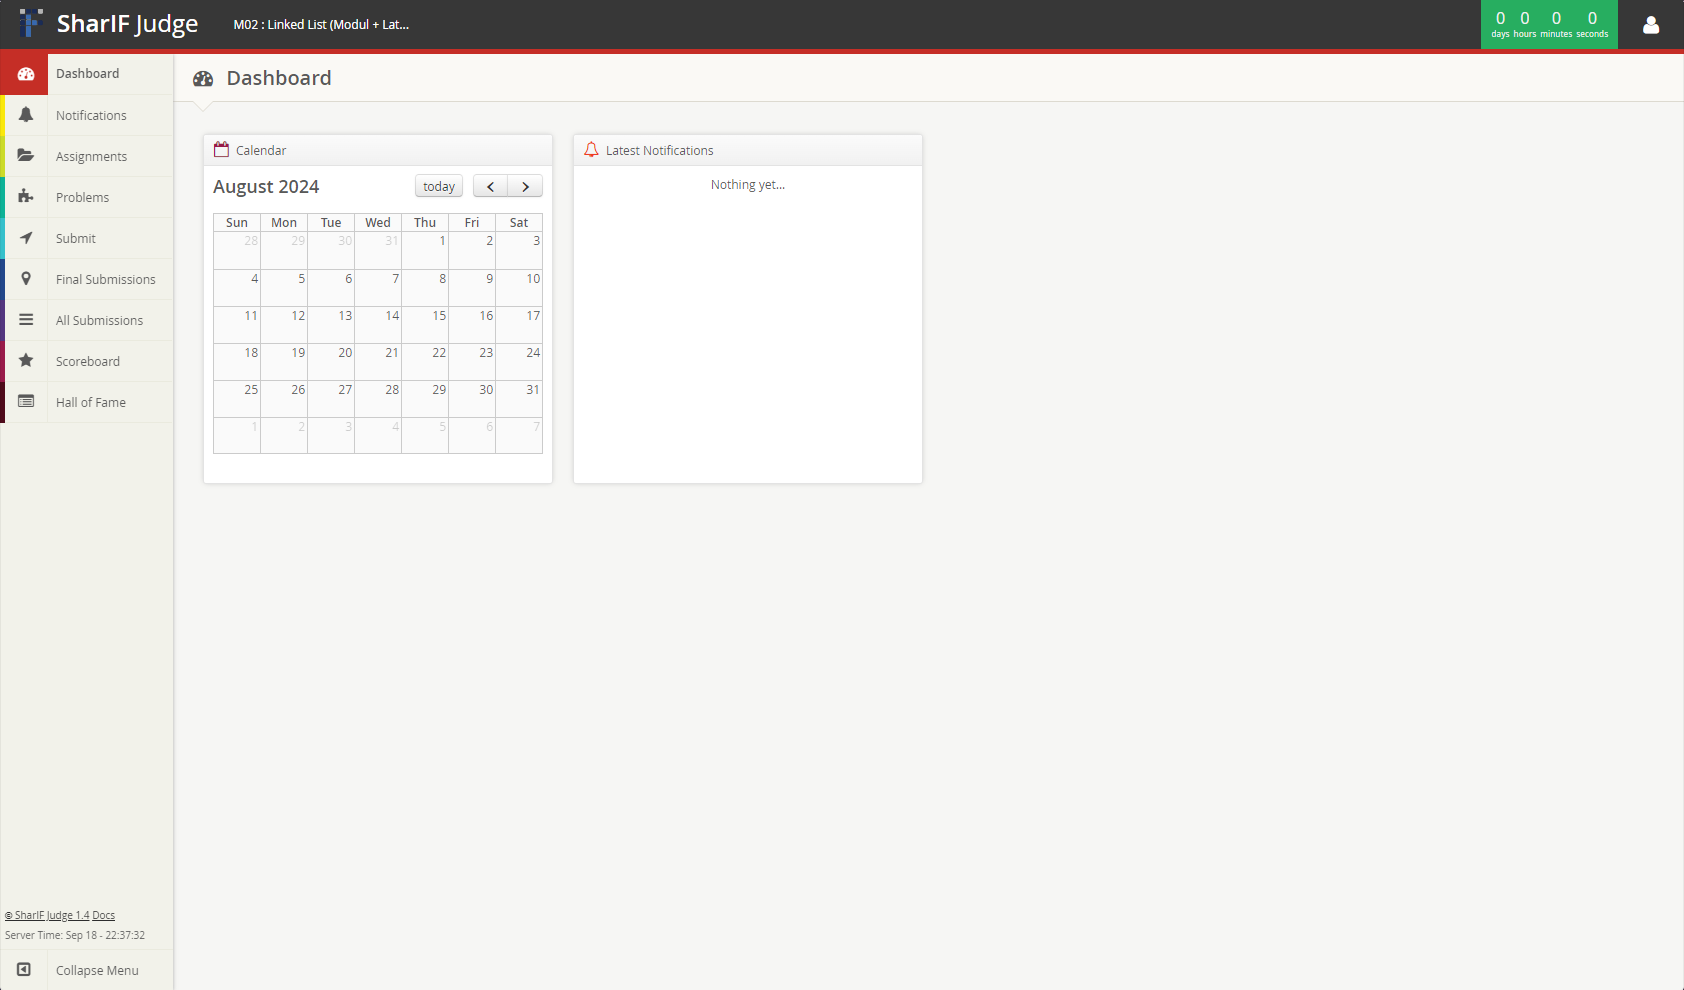
\includegraphics[width=\textwidth]{views/dashboard.png}
			            \caption{Halaman Dashboard}
			            \label{fig:3:1:1:dashboard}
		            \end{figure}

	      \end{itemize}

	\item \verb|Halloffame.php| \\
	      Berikut fungsi dengan penjelasannya pada \textit{controller} \verb|Halloffame.php|:

	      \begin{itemize}
		      \item \verb|hof_details()| \\
		            Menampilkan nilai akhir semua \textit{problem} dan \textit{assignments} pada sebuah \textit{user}.
		      \item \verb|index()| \\
		            Mendapatkan data dari \verb|Hof_model| dan mengembalikan \textit{view} \verb|halloffame.twig|. Gambar \ref{fig:3:1:1:hof} menunjukkan hasil halaman Hall of Fame yang dapat diakses oleh semua \textit{role}.

		            \begin{figure}[H]
			            \centering
			            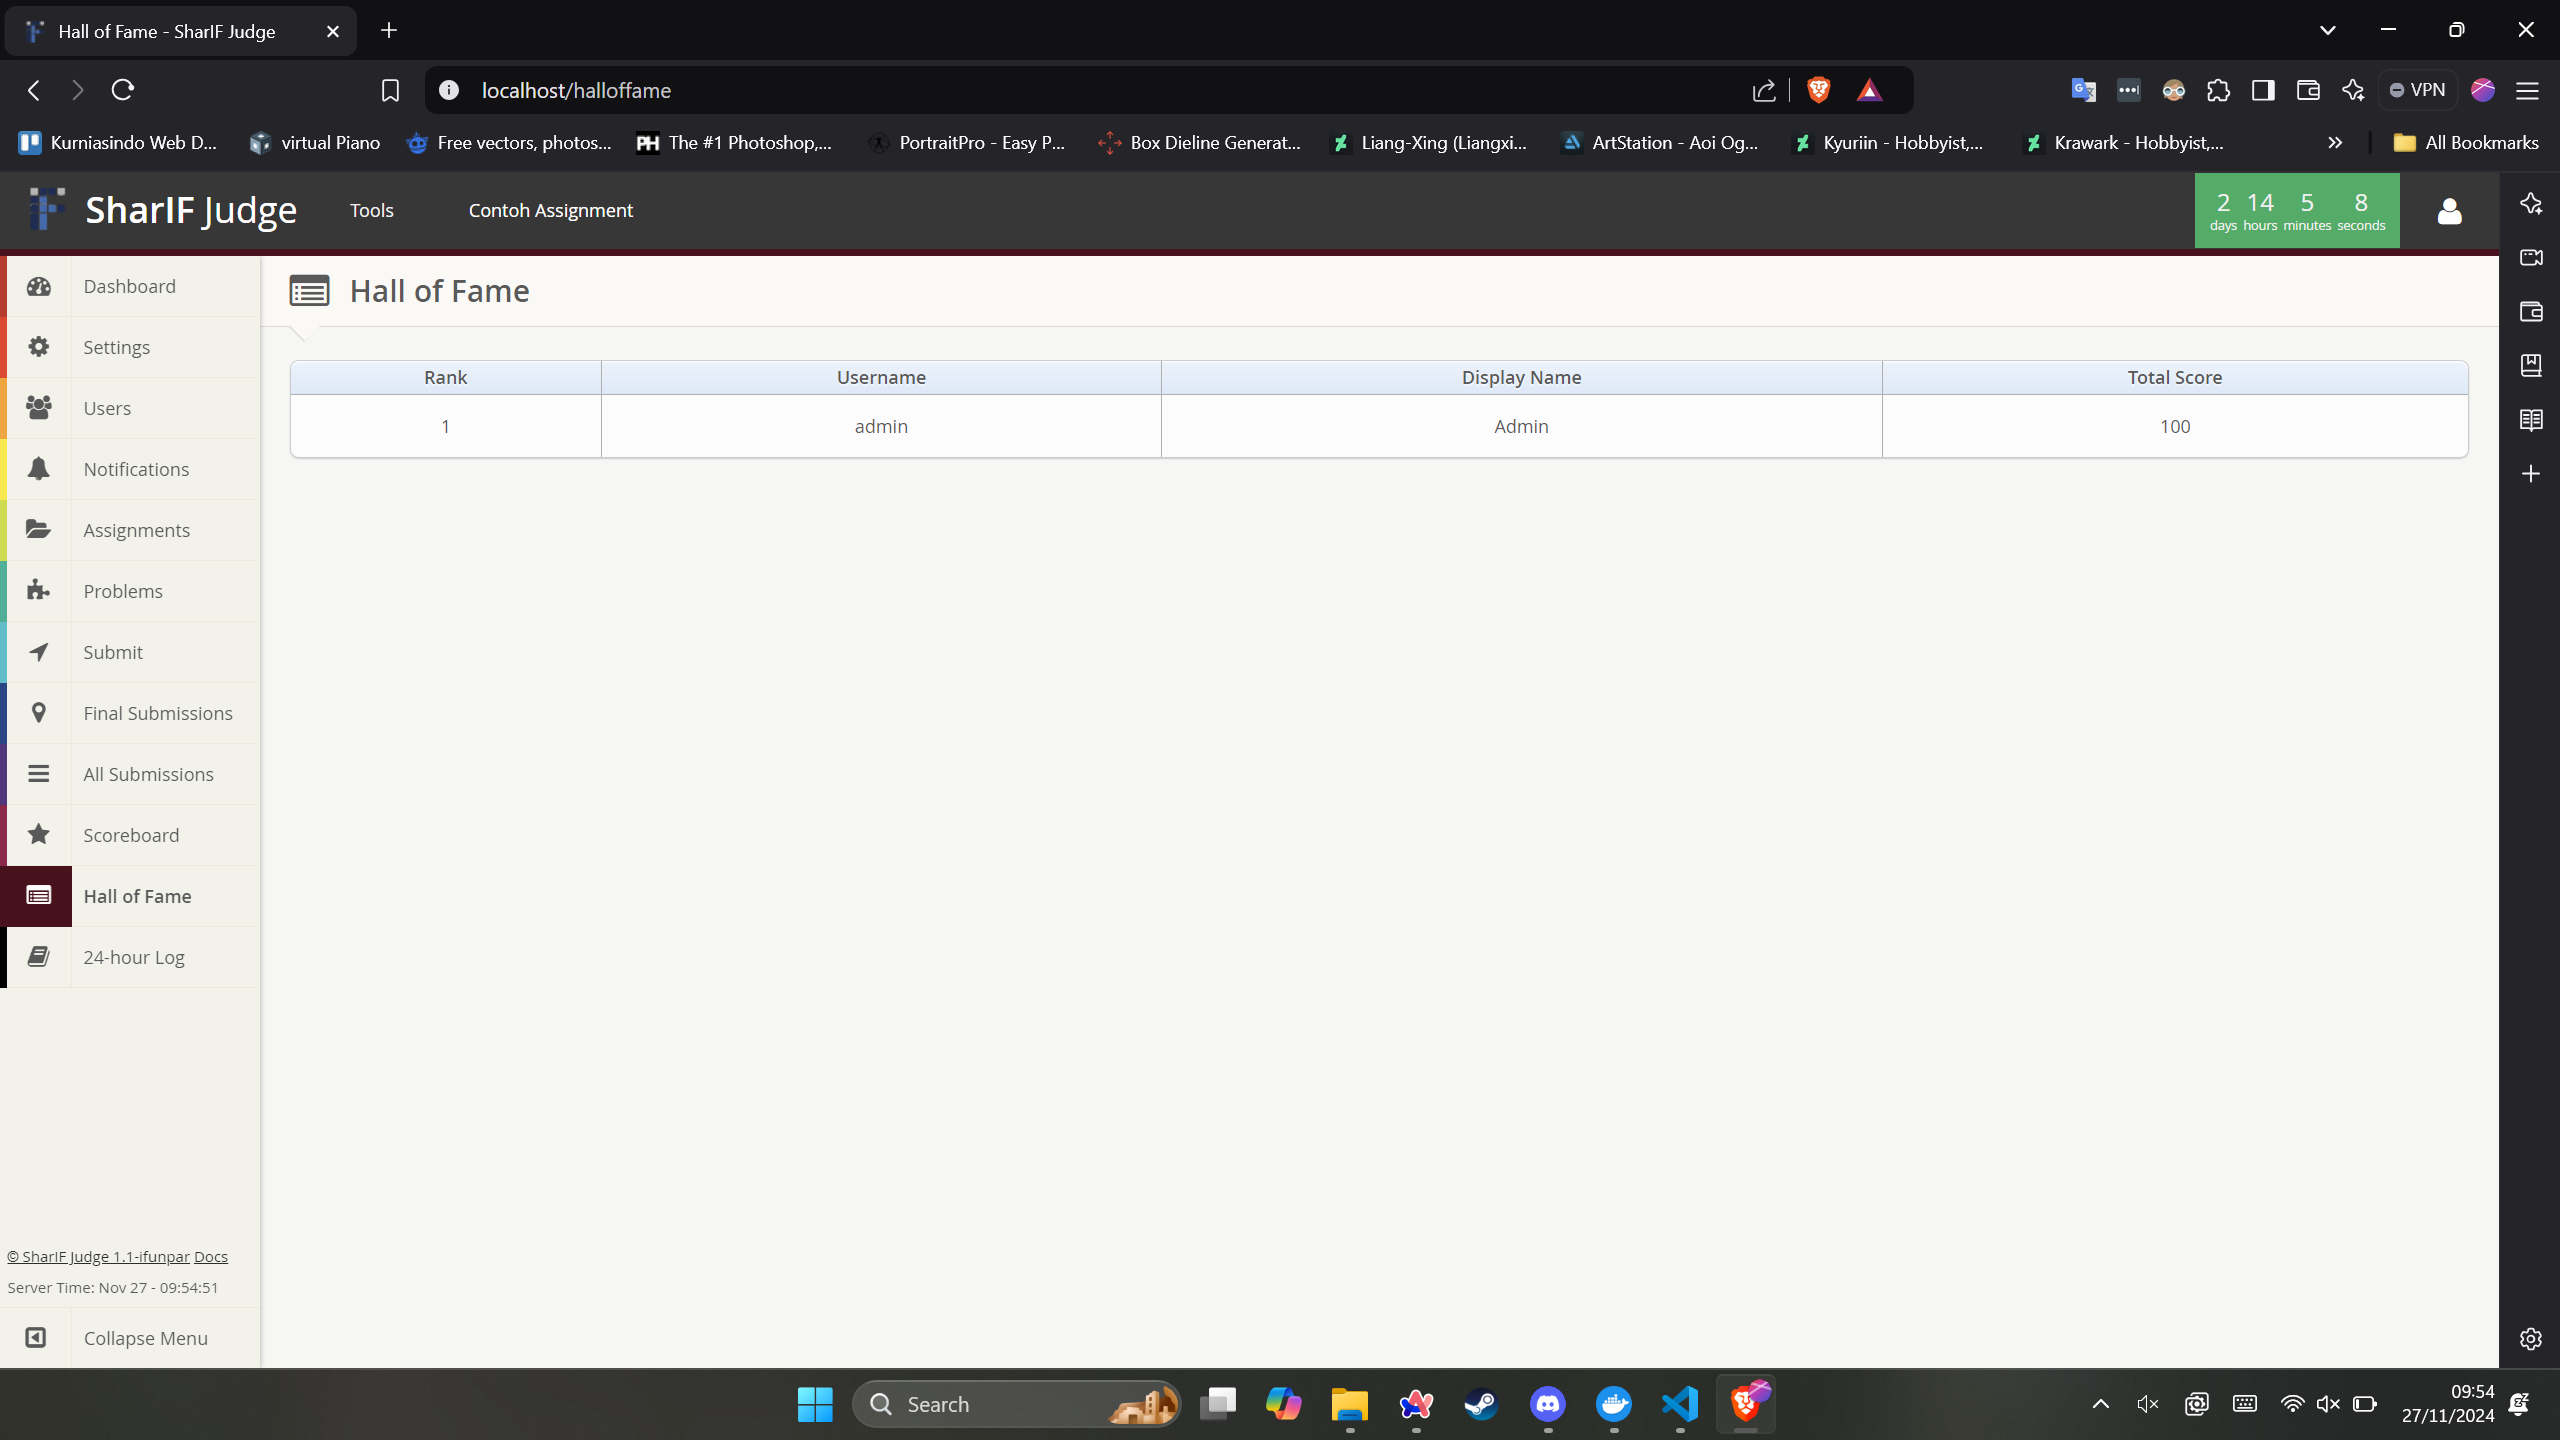
\includegraphics[width=\textwidth]{views/hof.png}
			            \caption{Halaman Hall of Fame}
			            \label{fig:3:1:1:hof}
		            \end{figure}

	      \end{itemize}

	\item \verb|Install.php| \\
	      Pada \textit{controller} \verb|Install.php| hanya ada satu fungsi yang menangani pembuatan seluruh tabel pada \textit{database} yang dibutuhkan oleh SharIF Judge. Setelah membuat \textit{database} akan mengembalikan \textit{view} \verb|install.twig| yang dapat diisi oleh pengguna tentang data \textit{user} dengan role \textit{admin} saat \textit{form} di kirim. Gambar \ref{fig:3:1:1:install} menunjukkan hasil halaman Install.

	      \begin{figure}[H]
		      \centering
		      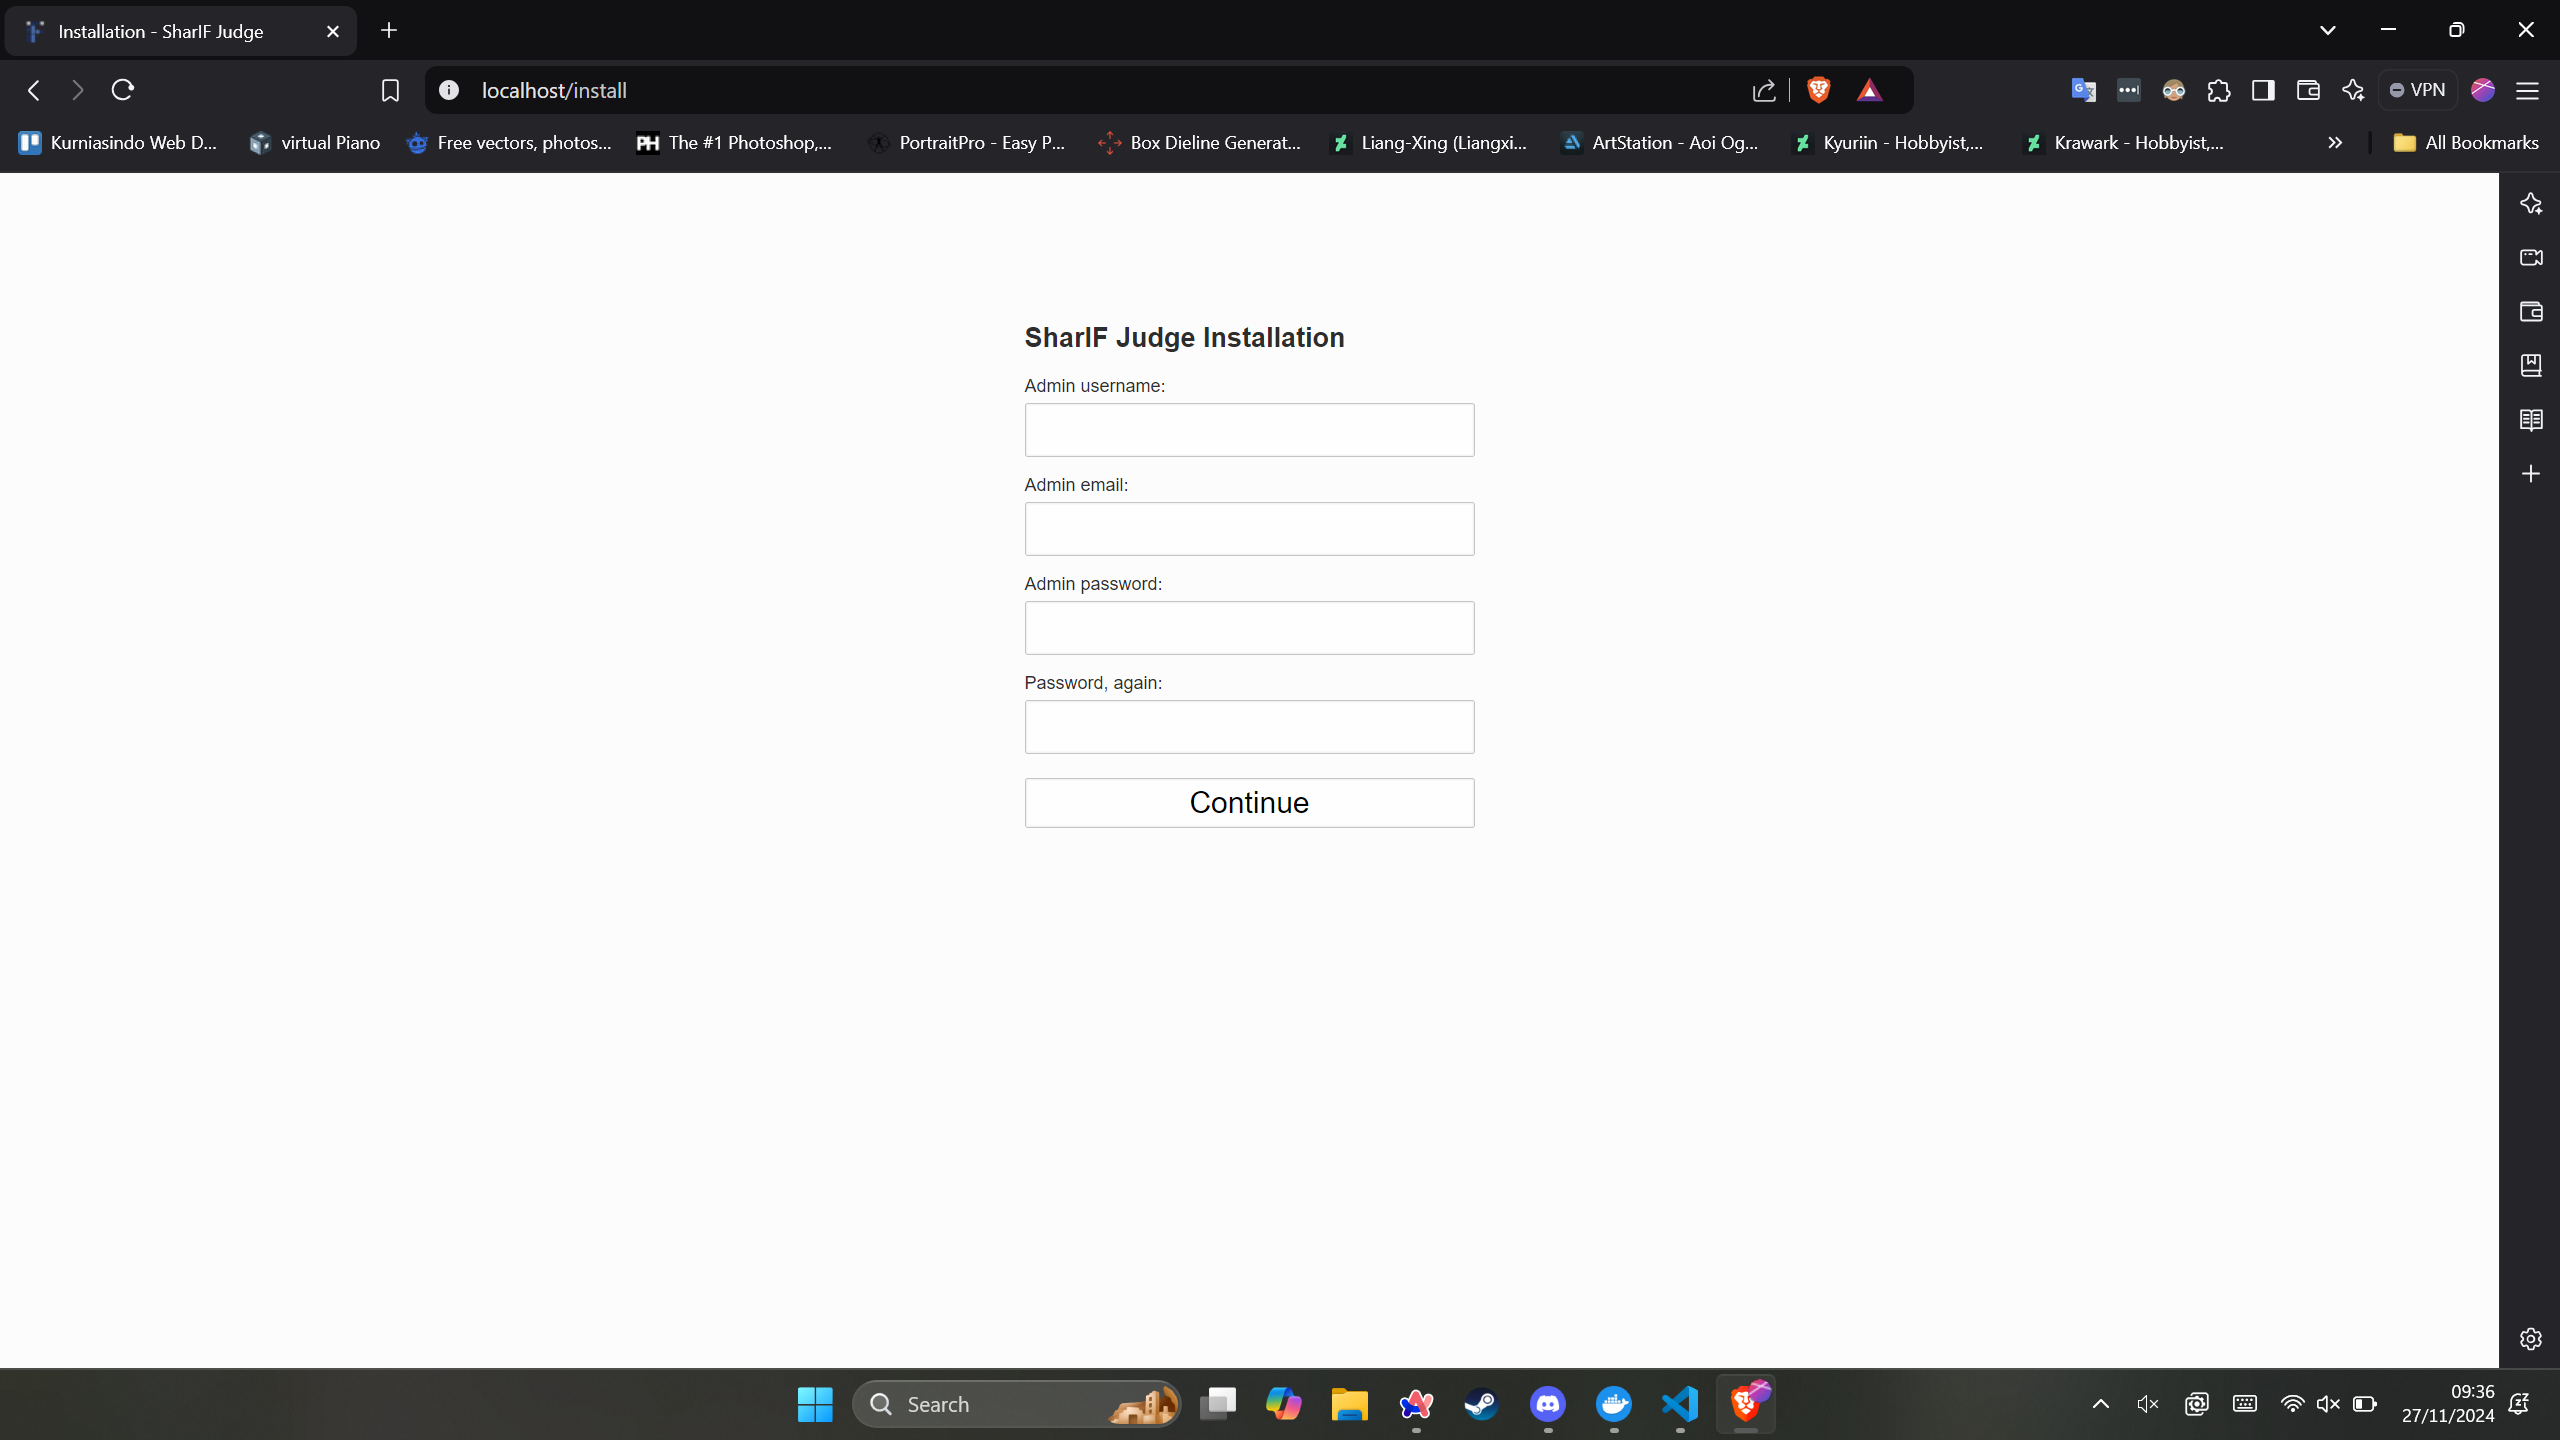
\includegraphics[width=\textwidth]{views/install.png}
		      \caption{Halaman Install}
		      \label{fig:3:1:1:install}
	      \end{figure}


	\item \verb|Login.php| \\
	      Berikut fungsi dengan penjelasannya pada \textit{controller} \verb|Login.php|:

	      \begin{itemize}
		      \item \verb|_registration_code($code)| \\
		            Melakukan validasi kode registrasi.
		      \item \verb|register()| \\
		            Menunjukkan halaman \verb|register.twig| dan membuat \textit{user} baru.
		      \item \verb|logout()| \\
		            Melakukan \textit{Log out} dan mengalihkan ke halaman \textit{login}.
		      \item \verb|lost()| \\
		            Mengirimkan email \textit{reset password}.
		      \item \verb|reset($passchange_key)| \\
		            Melakukan \textit{reset password} dengan halaman \verb|reset_password.twig|.
		      \item \verb|index()| \\
		            Mengembalikan \textit{view} \verb|login.twig| dan memeriksa username dan password pada \textit{form} saat di kirim. Gambar \ref{fig:3:1:1:login} menunjukkan hasil halaman Login.

		            \begin{figure}[H]
			            \centering
			            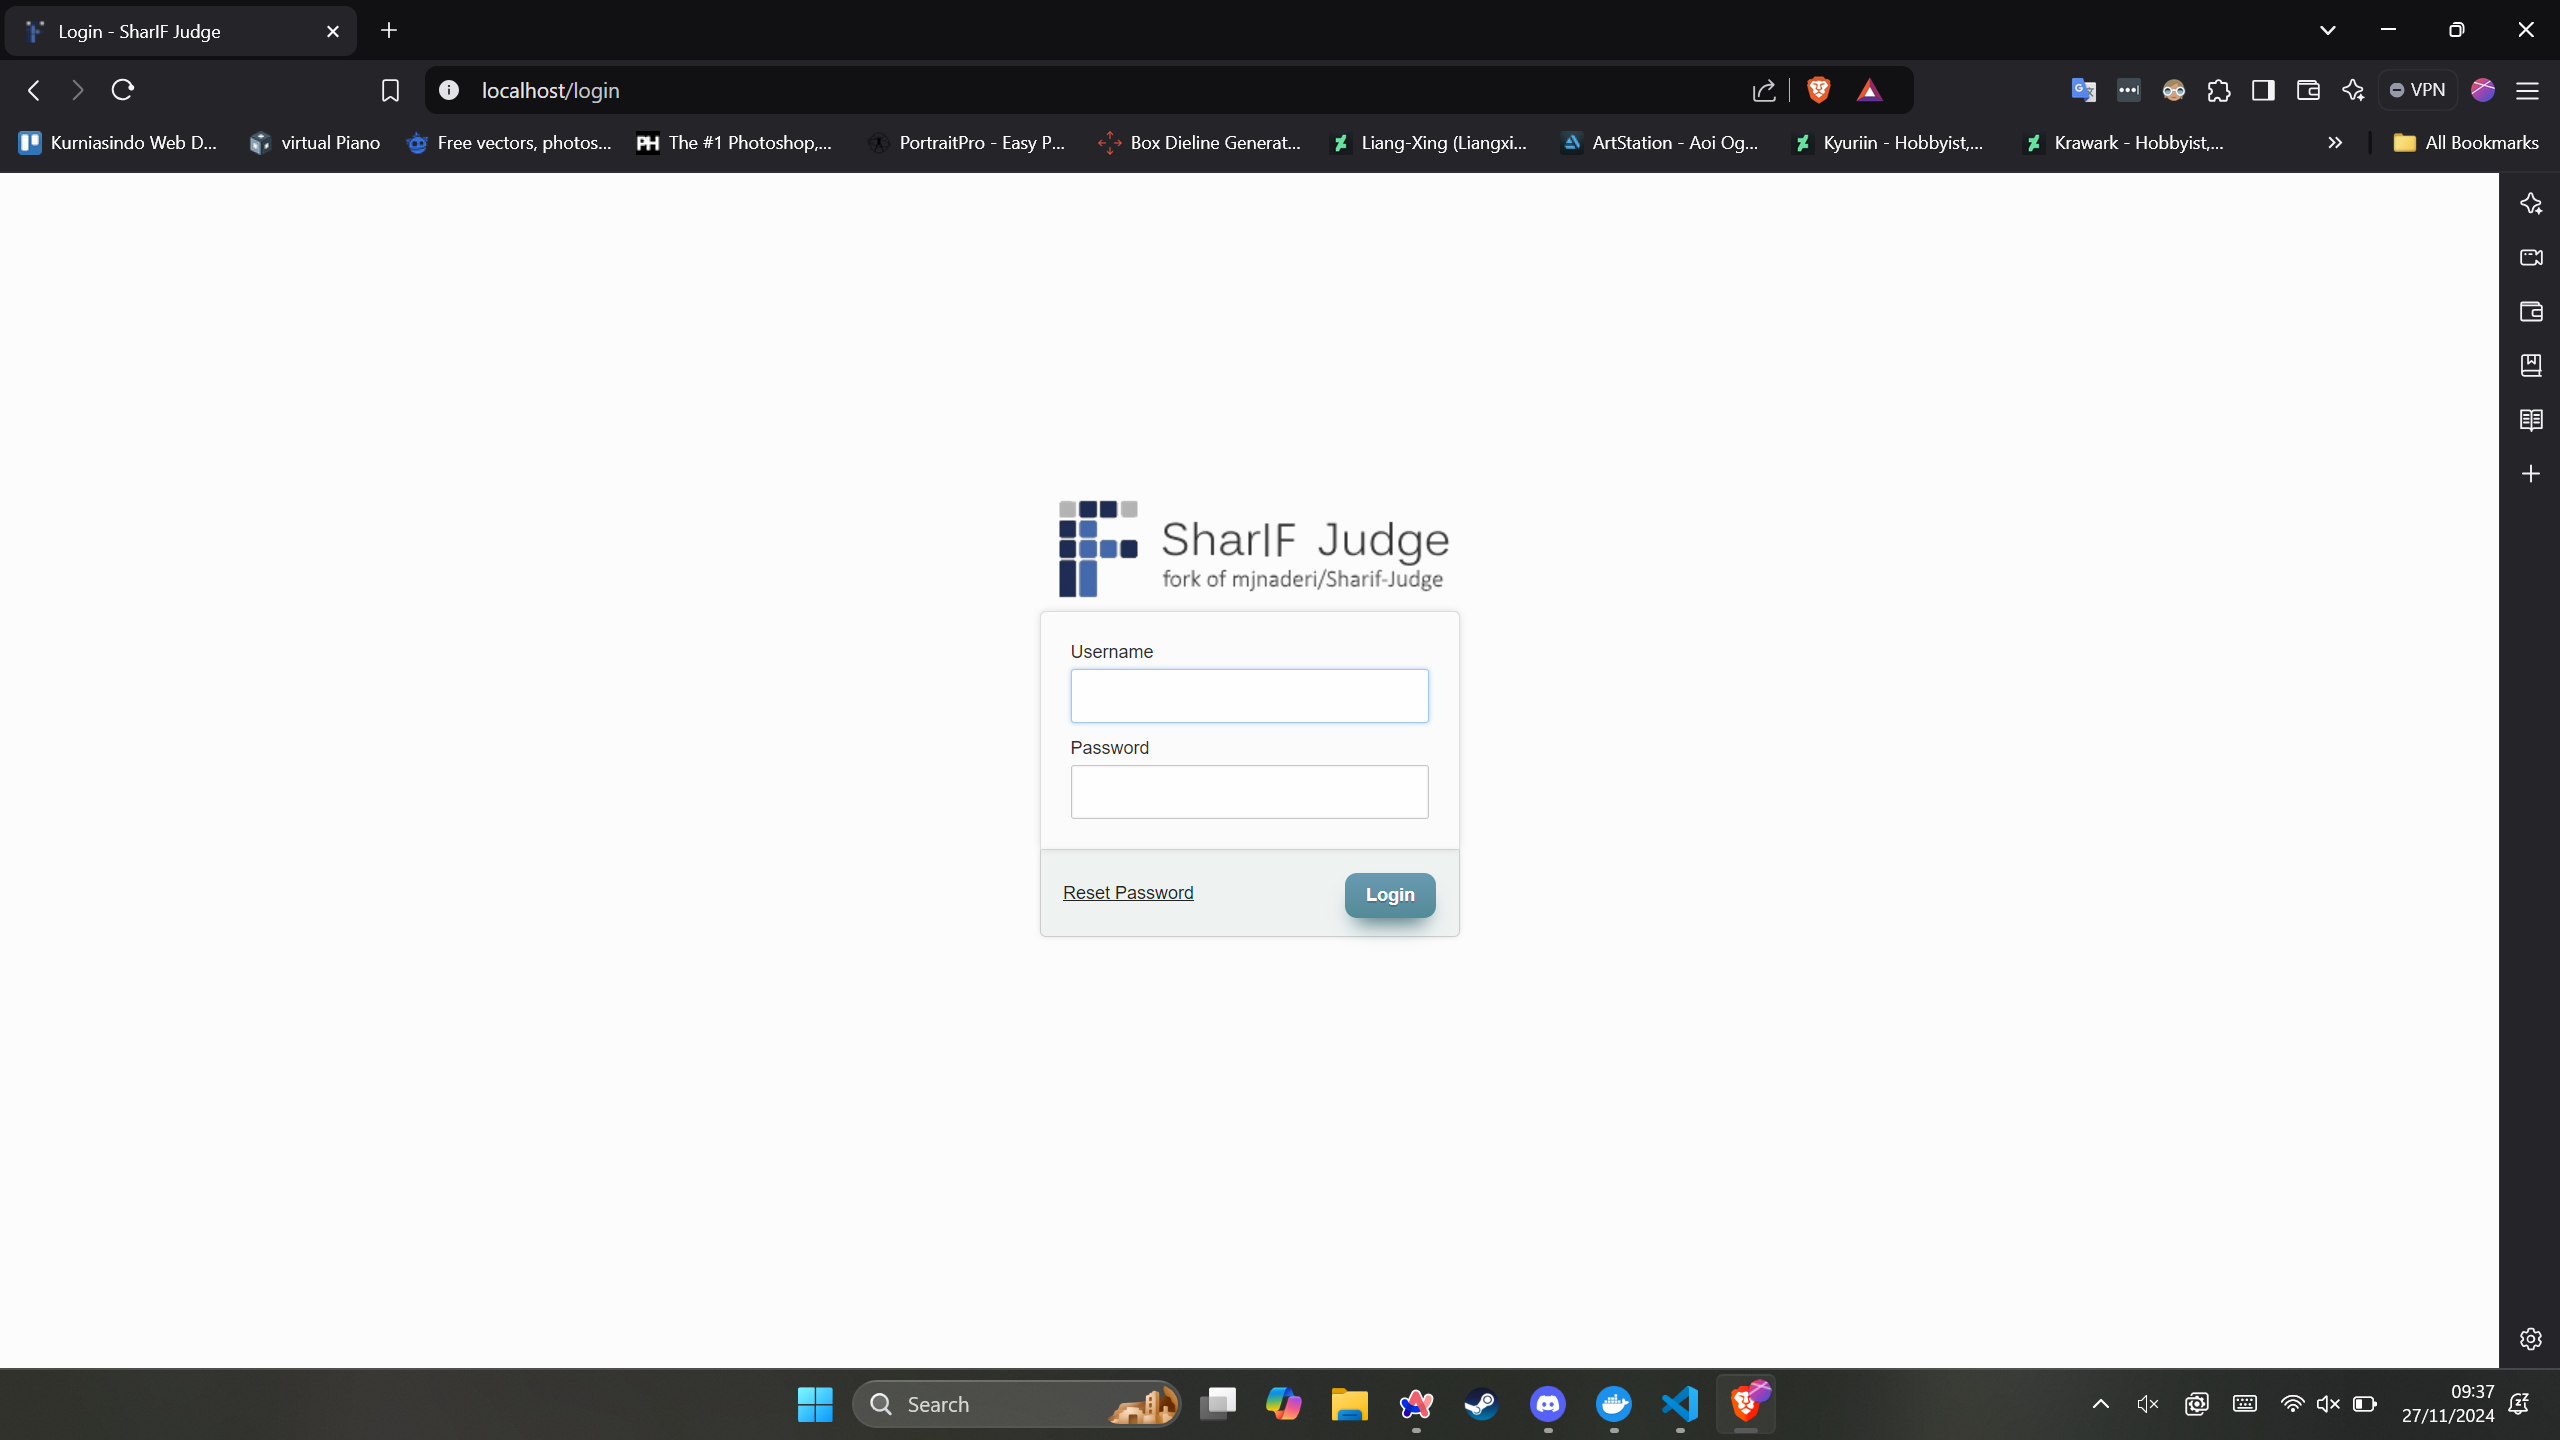
\includegraphics[width=\textwidth]{views/login.png}
			            \caption{Halaman Login}
			            \label{fig:3:1:1:login}
		            \end{figure}

	      \end{itemize}

	\item \verb|Logs.php| \\
	      Pada \textit{controller} \verb|Logs.php| hanya memiliki satu fungsi yaitu \verb|index()|, dimana fungsi tersebut akan mendapatkan data dari \verb|Logs_model| dan memunculkan halaman \verb|logs.twig|. Gambar \ref{fig:3:1:1:log} menunjukkan halaman Log yang dinamakan halaman 24-Hour Log.

	      \begin{figure}[H]
		      \centering
		      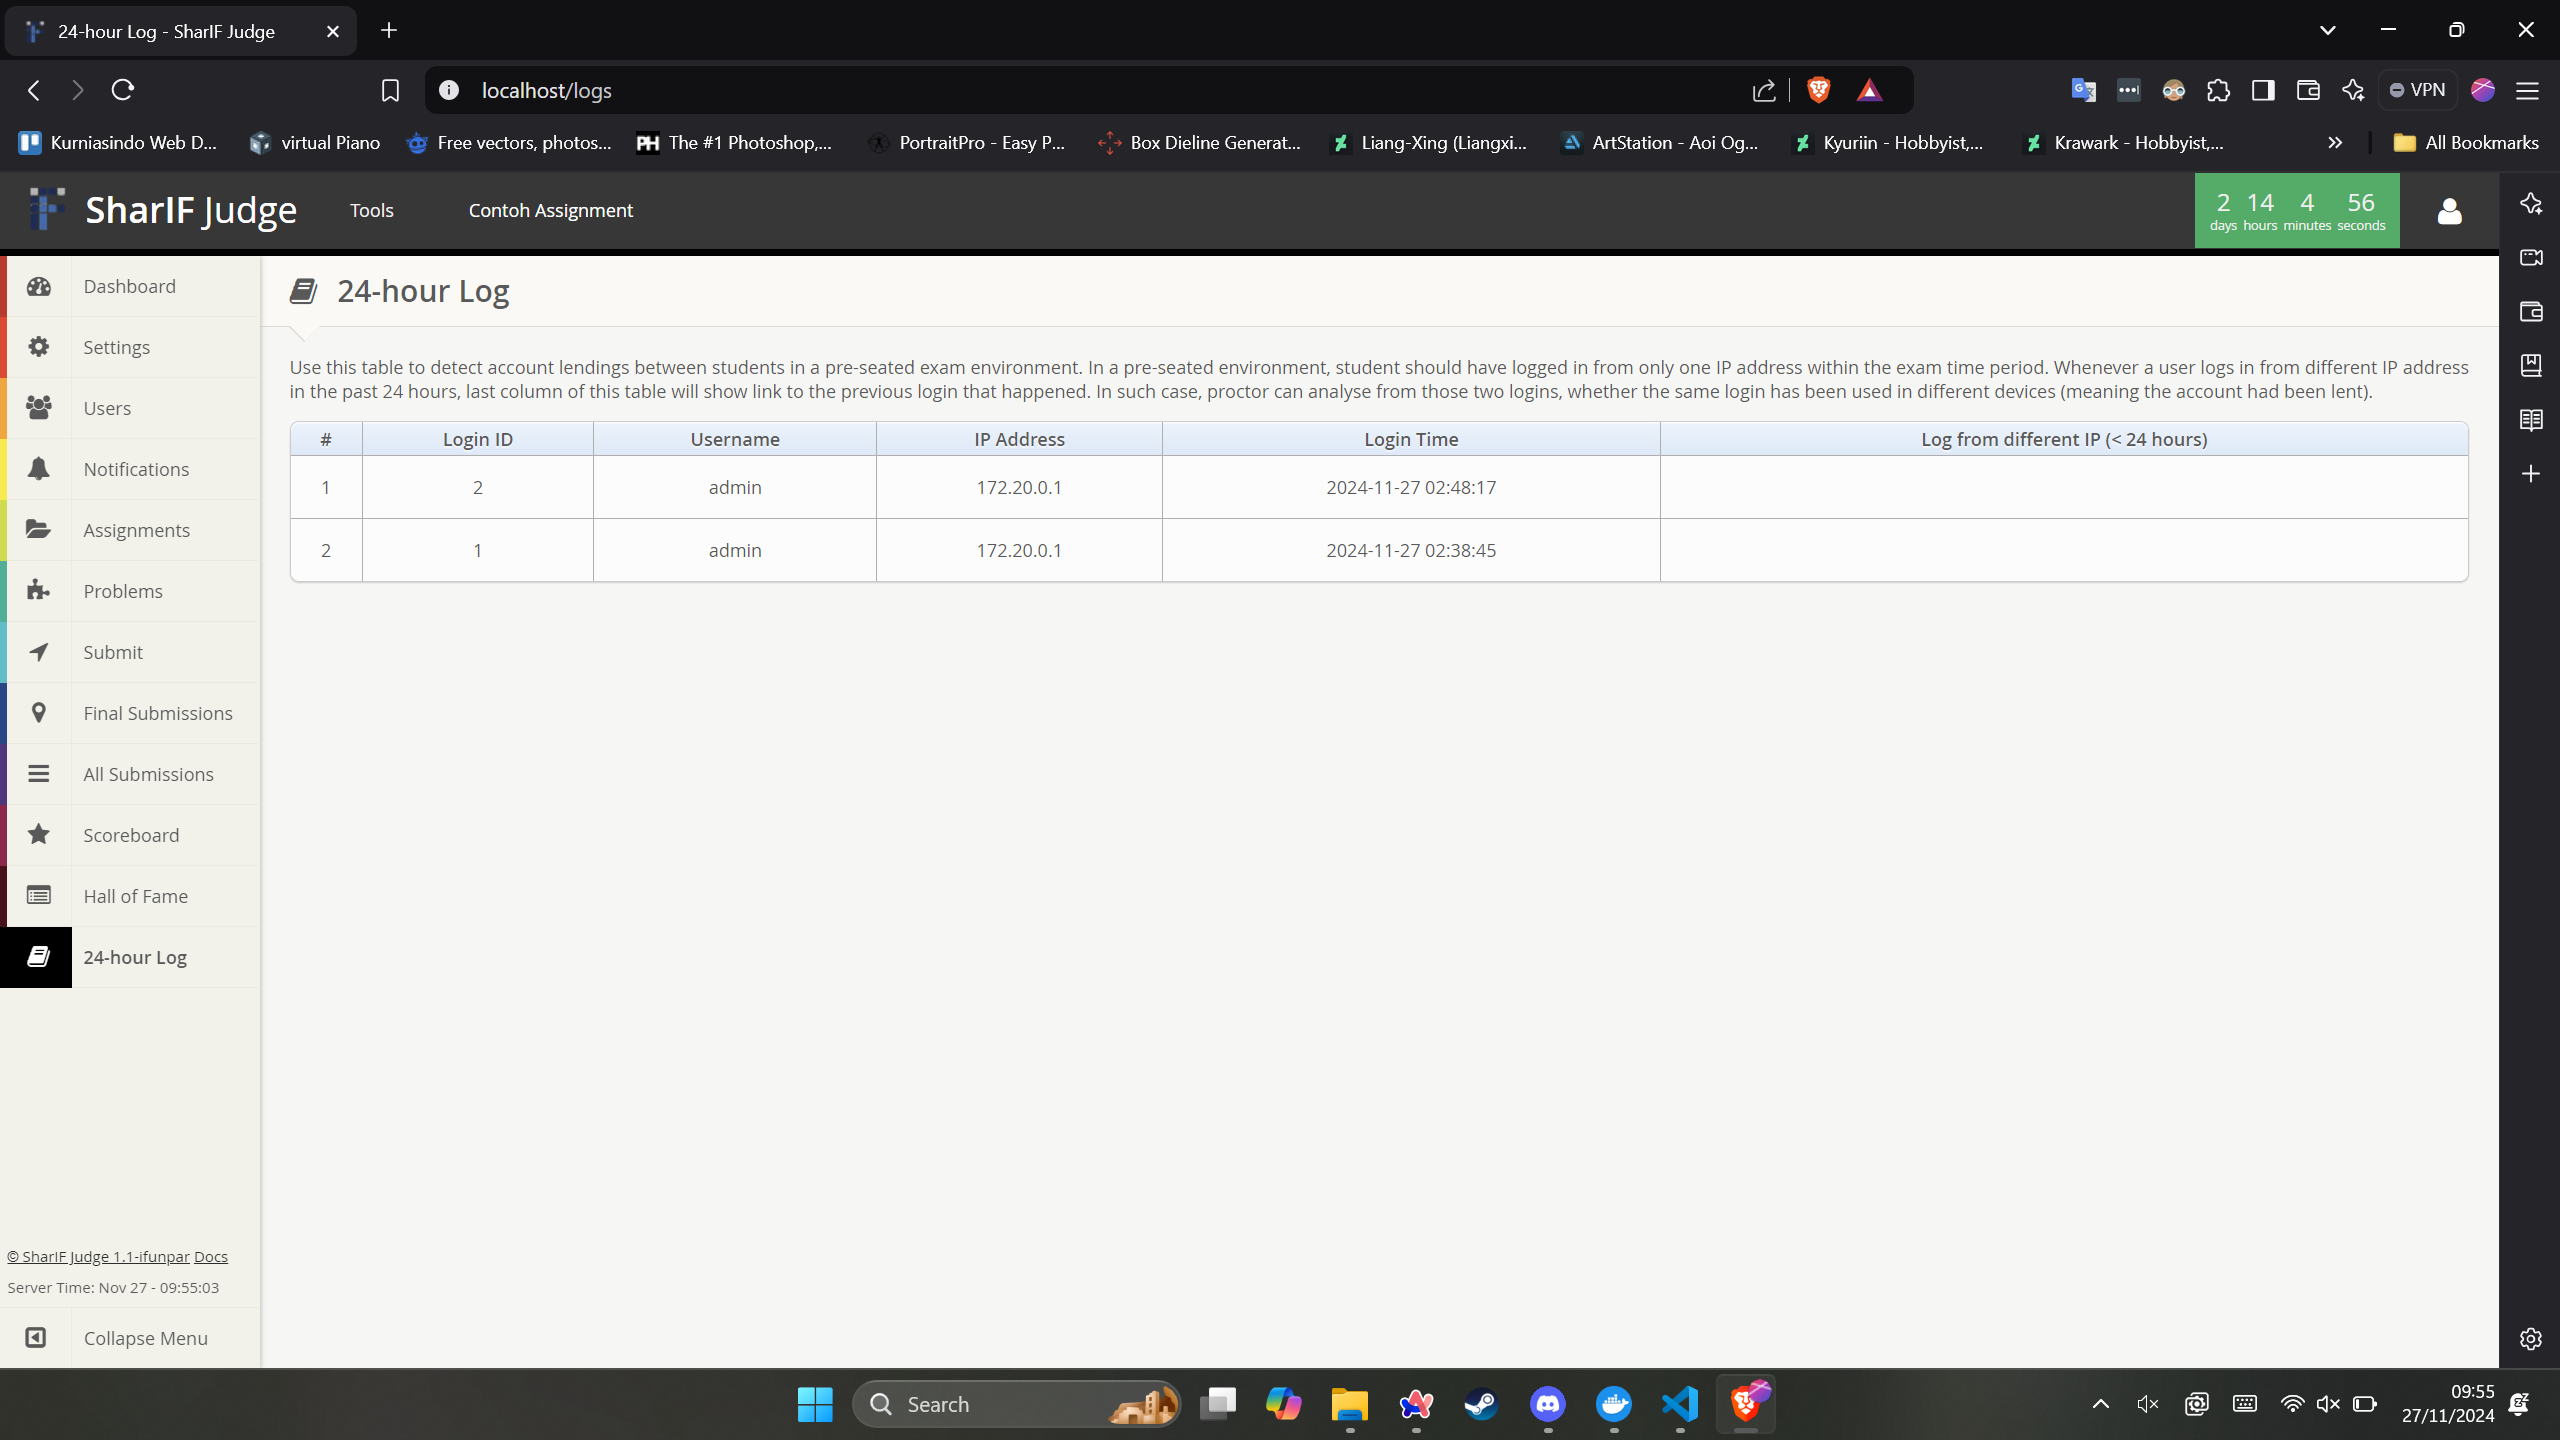
\includegraphics[width=\textwidth]{views/log.png}
		      \caption{Halaman 24-Hour Log}
		      \label{fig:3:1:1:log}
	      \end{figure}


	\item \verb|Moss.php| \\
	      Berikut fungsi dengan penjelasannya pada \textit{controller} \verb|Moss.php|:

	      \begin{itemize}
		      \item \verb|update($assignment_id)| \\
		            Memperbaharui \textit{settings} dari masukkan \verb|moss_userid| pengguna.
		      \item \verb|_detect($assignment_id)| \\
		            Melakukan pemeriksaan kesamaan kode dengan Moss.
		      \item \verb|index()| \\
		            Mengambil data dan memasukkannya ke dalam \textit{view} \verb|moss.twig|. Gambar \ref{fig:3:1:1:moss} merupakan hasil halaman moss. Fungsi \verb|_detect| juga akan dijalankan saat \textit{form} terkirim.

		            \begin{figure}[H]
			            \centering
			            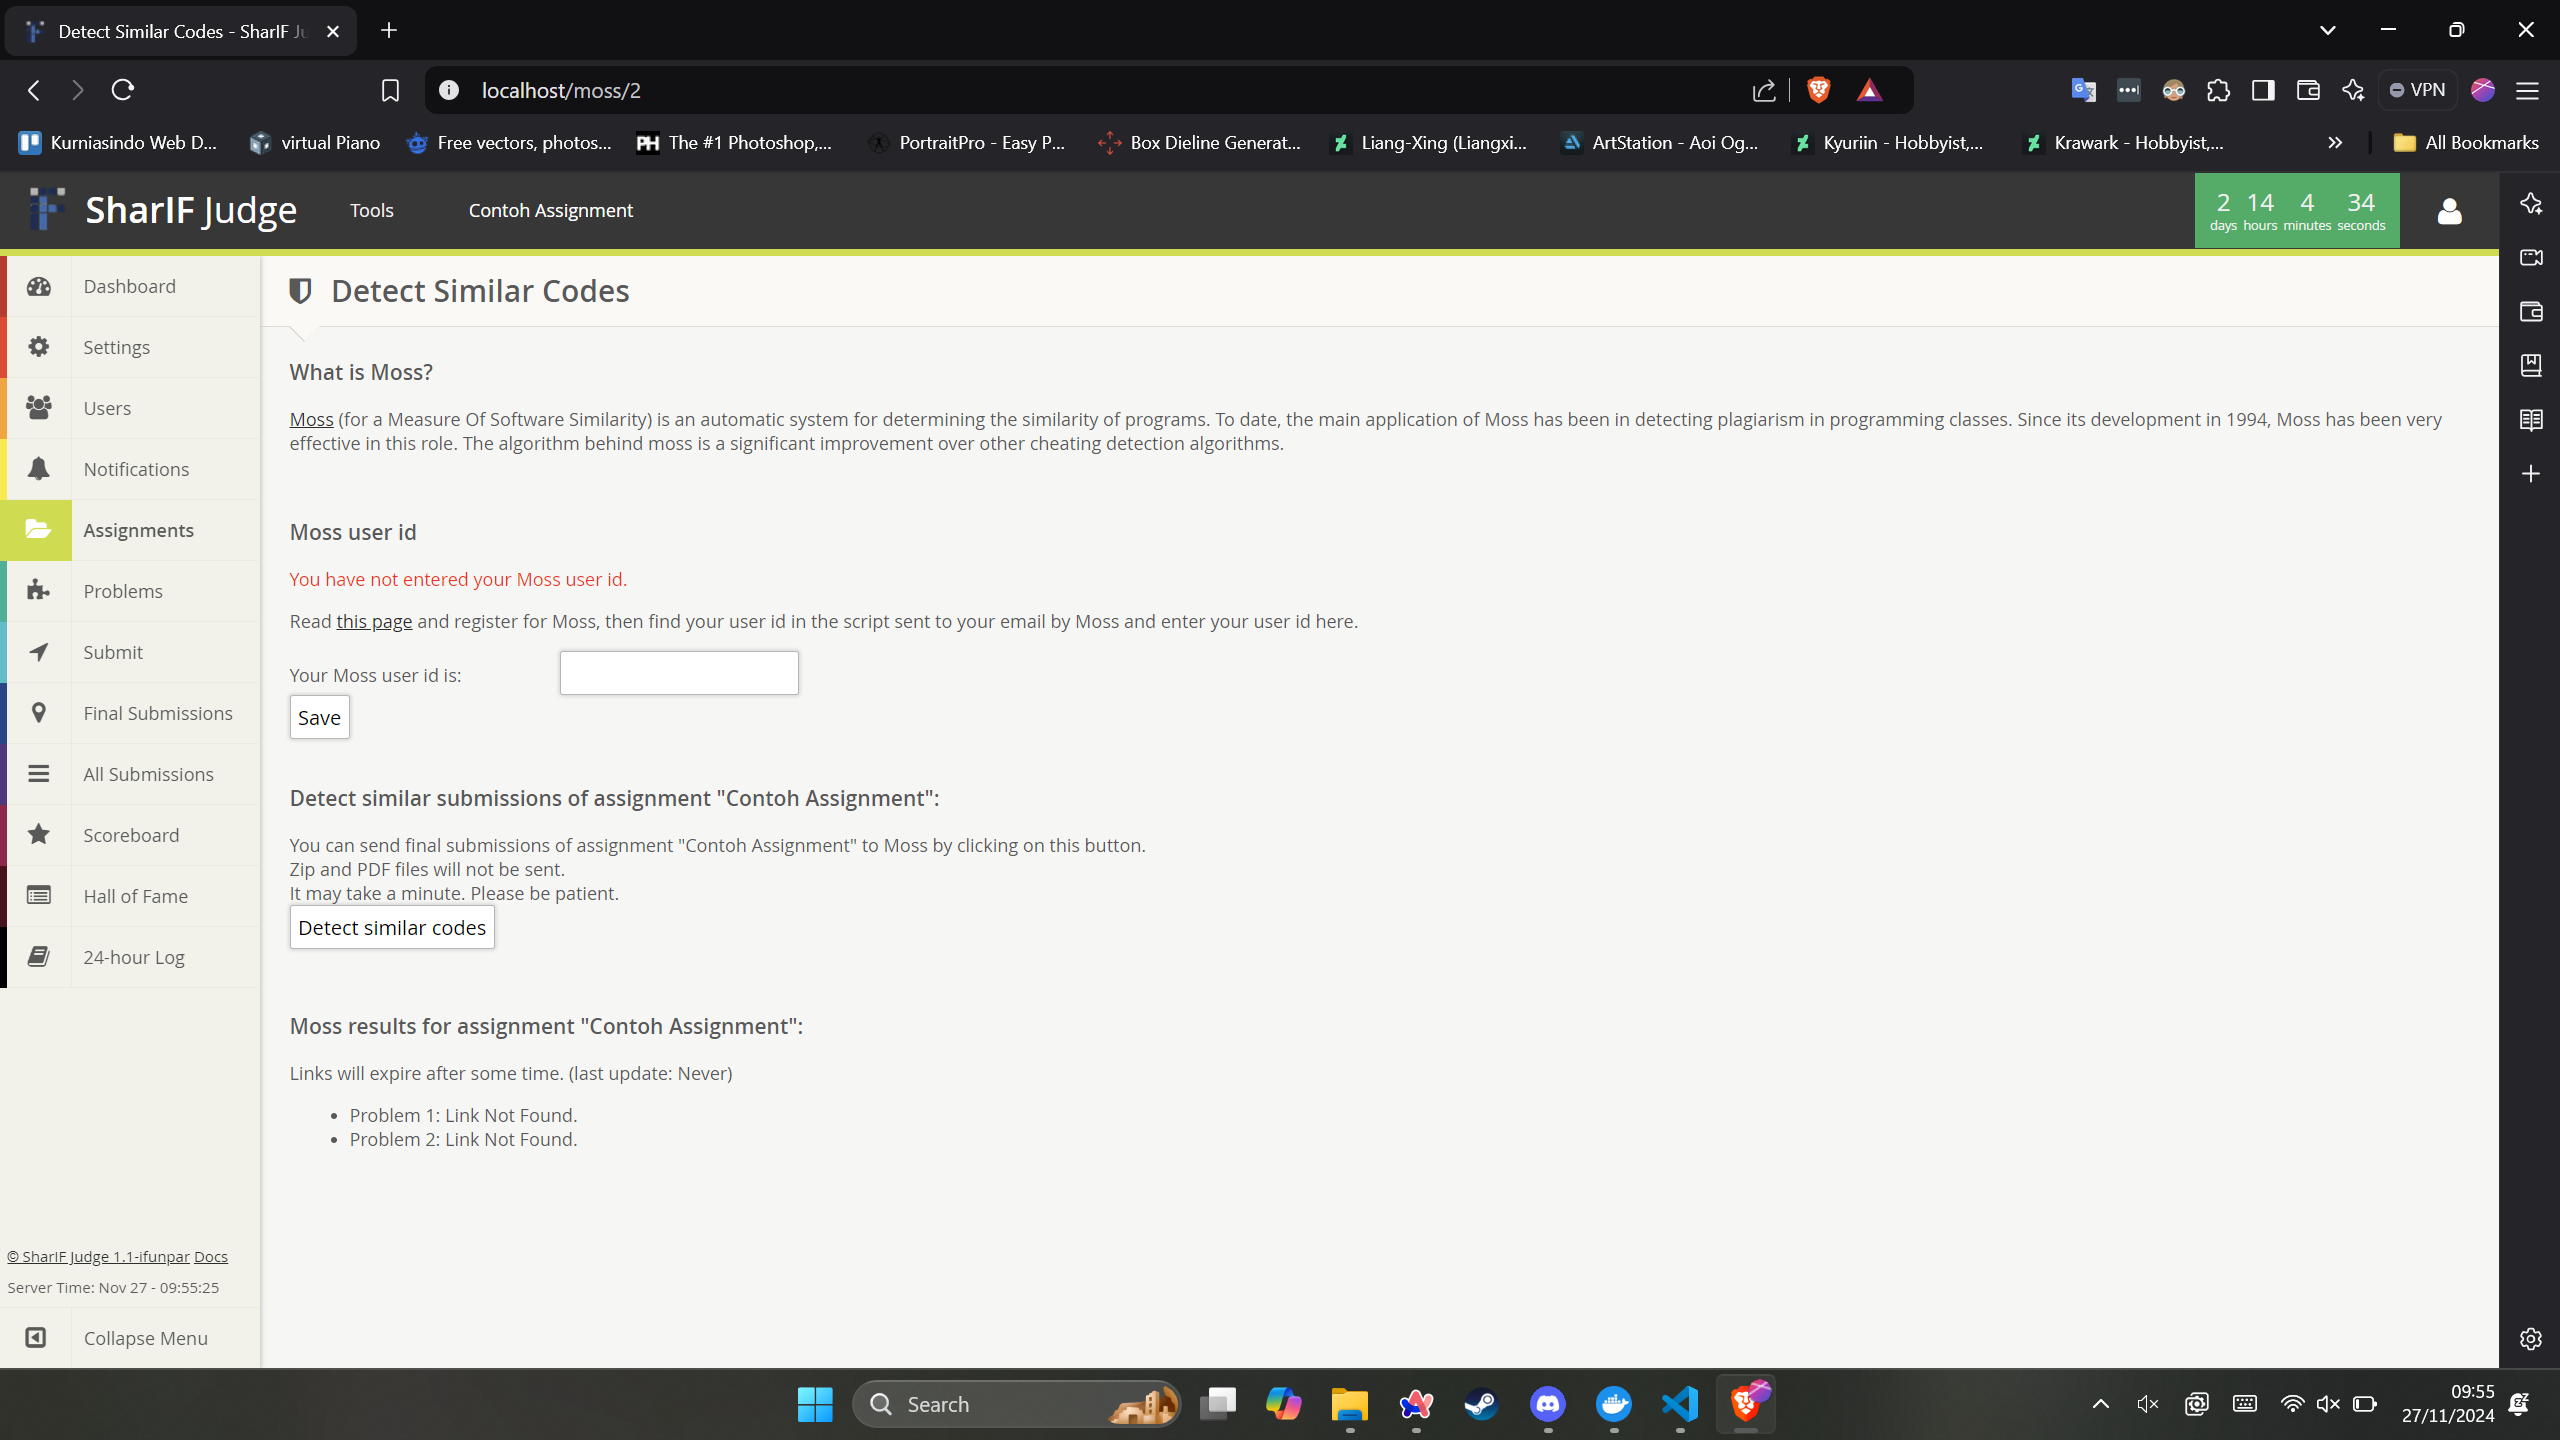
\includegraphics[width=\textwidth]{views/moss.png}
			            \caption{Halaman Moss}
			            \label{fig:3:1:1:moss}
		            \end{figure}

	      \end{itemize}

	\item \verb|Notifications.php| \\
	      Berikut fungsi dengan penjelasannya pada \textit{controller} \verb|Notifications.php|:

	      \begin{itemize}
		      \item \verb|add()| \\
		            Menambahkan atau memperbaharui sebuah \textit{notification}.
		      \item \verb|edit($notif_id)| \\
		            Menandai \textit{notification} yang akan di \textit{edit} dan memanggil fungsi \verb|add|.
		      \item \verb|delete()| \\
		            Menghapus sebuah \textit{notification}.
		      \item \verb|check()| \\
		            Mengunakan \textit{ajax request} untuk mengetahui ketersediaan \textit{notification} baru.
		      \item \verb|index()| \\
		            Mendapatkan data dari dua model yaitu \verb|Assignment_model| dan \verb|Notifications_model|. Data akan dimasukkan ke dalam \textit{view} \verb|notifications.twig| yang akan dikembalikan ke pengguna. Gambar \ref{fig:3:1:1:notif} menunjukkan hasil halaman \textit{Notifications}.

		            \begin{figure}[H]
			            \centering
			            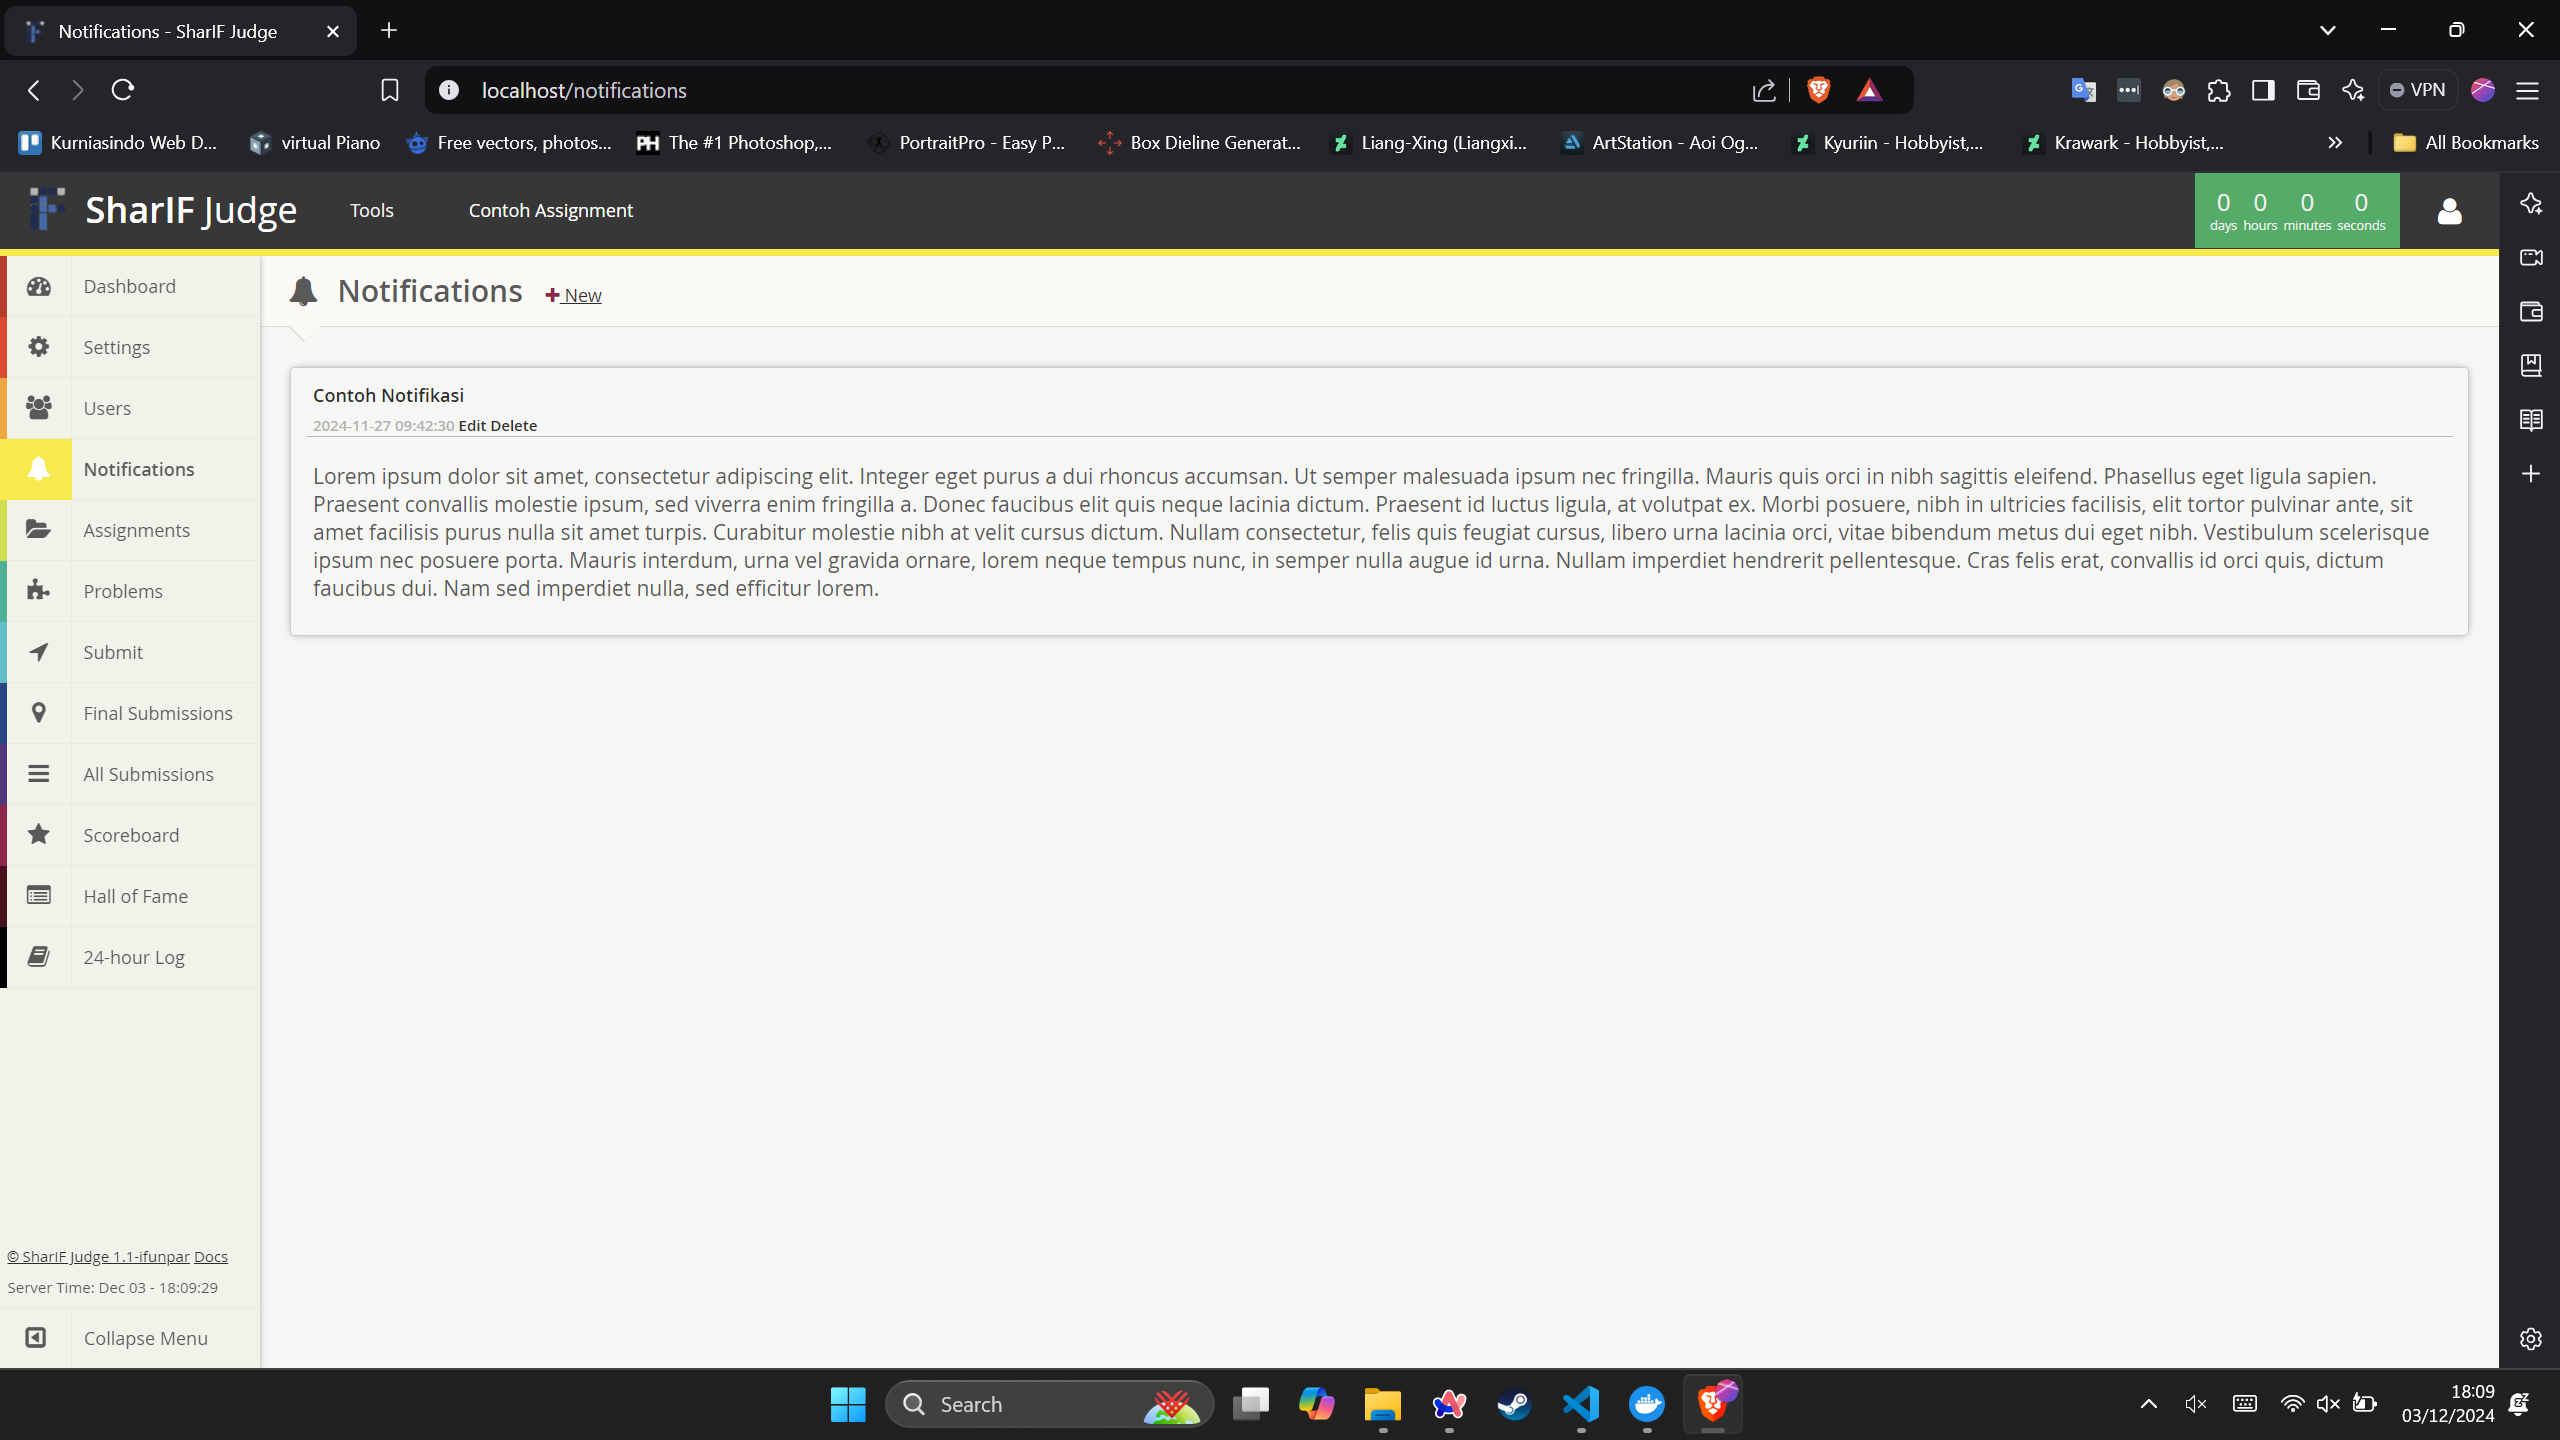
\includegraphics[width=\textwidth]{views/notifications.png}
			            \caption{Halaman Notifications}
			            \label{fig:3:1:1:notif}
		            \end{figure}

	      \end{itemize}

	\item \verb|Problems.php| \\
	      Berikut fungsi dengan penjelasannya pada \textit{controller} \verb|Notifications.php|:

	      \begin{itemize}
		      \item \verb|edit()| \\
		            Memperbaharui deskripsi sebuah \textit{problem} dalam bentuk \verb|html| atau \verb|markdown|.
		      \item \verb|index()| \\
		            Mendapatkan data \textit{problem} dari berbagai \textit{model} sesuai dengan \textit{assignment} yang dipilih dan menaruh data tersebut pada halaman \verb|problems.twig| yang akan ditampilkan ke pengguna. Gambar \ref{fig:3:1:1:problem} menunjukkan hasil halaman Problems.

		            \begin{figure}[H]
			            \centering
			            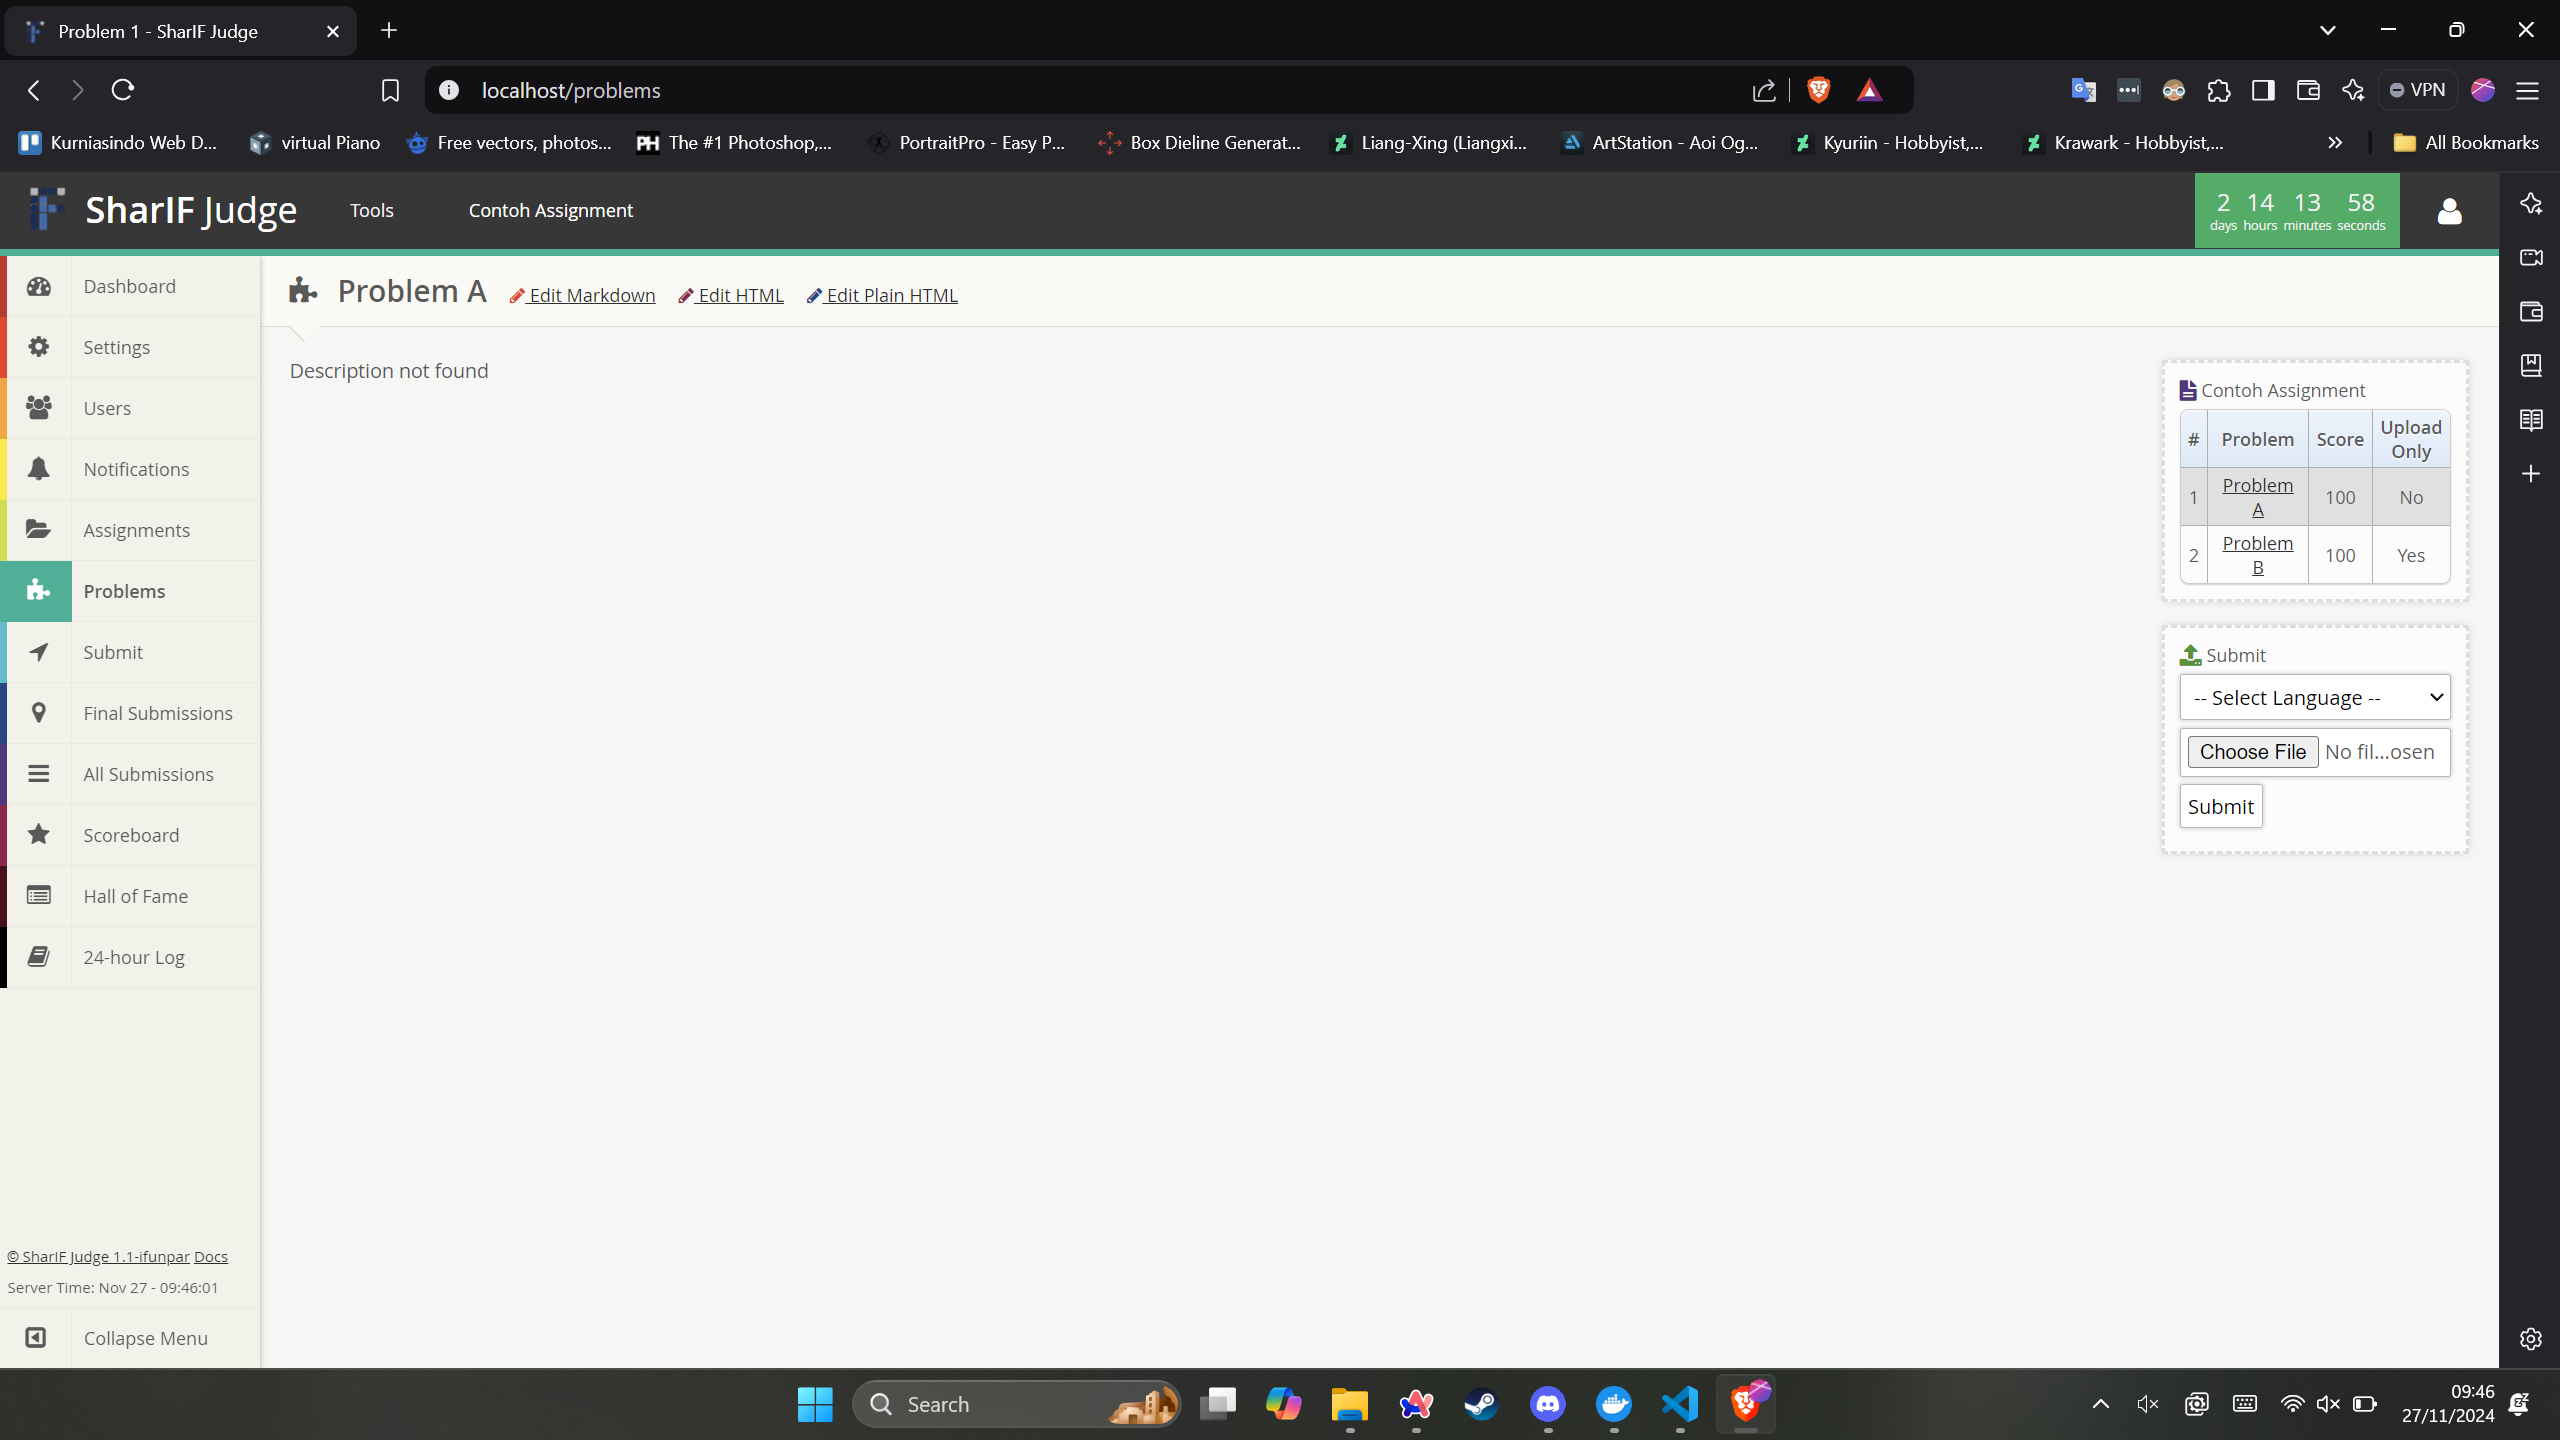
\includegraphics[width=\textwidth]{views/problem.png}
			            \caption{Halaman Problems}
			            \label{fig:3:1:1:problem}
		            \end{figure}

	      \end{itemize}

	\item \verb|Profile.php| \\
	      Berikut fungsi dengan penjelasannya pada \textit{controller} \verb|Profile.php|:

	      \begin{itemize}
		      \item \verb|_password_check($str)| \\
		            Melakukan validasi \textit{input password}.
		      \item \verb|_password_again_check($str)| \\
		            Melakukan validasi \textit{input} tulisan pengulangan \textit{password}.
		      \item \verb|_email_check($str)| \\
		            Melakukan validasi ketersediaan email pada \textit{database}.
		      \item \verb|_role_check($str)| \\
		            Melakukan validasi \textit{role} pengguna saat ingin mengubah \textit{role user}.
		      \item \verb|index()| \\
		            Mendapatkan data dari berbagai \textit{model} terutama dari \textit{User} yang akan dimasukkan ke dalam \textit{view} \verb|profile.twig|. Fungsi ini juga menangani pengiriman \textit{form} pembaharuan data \textit{user} pengguna. Gambar \ref{fig:3:1:1:profile} menunjukkan hasil halaman Profile.

		            \begin{figure}[H]
			            \centering
			            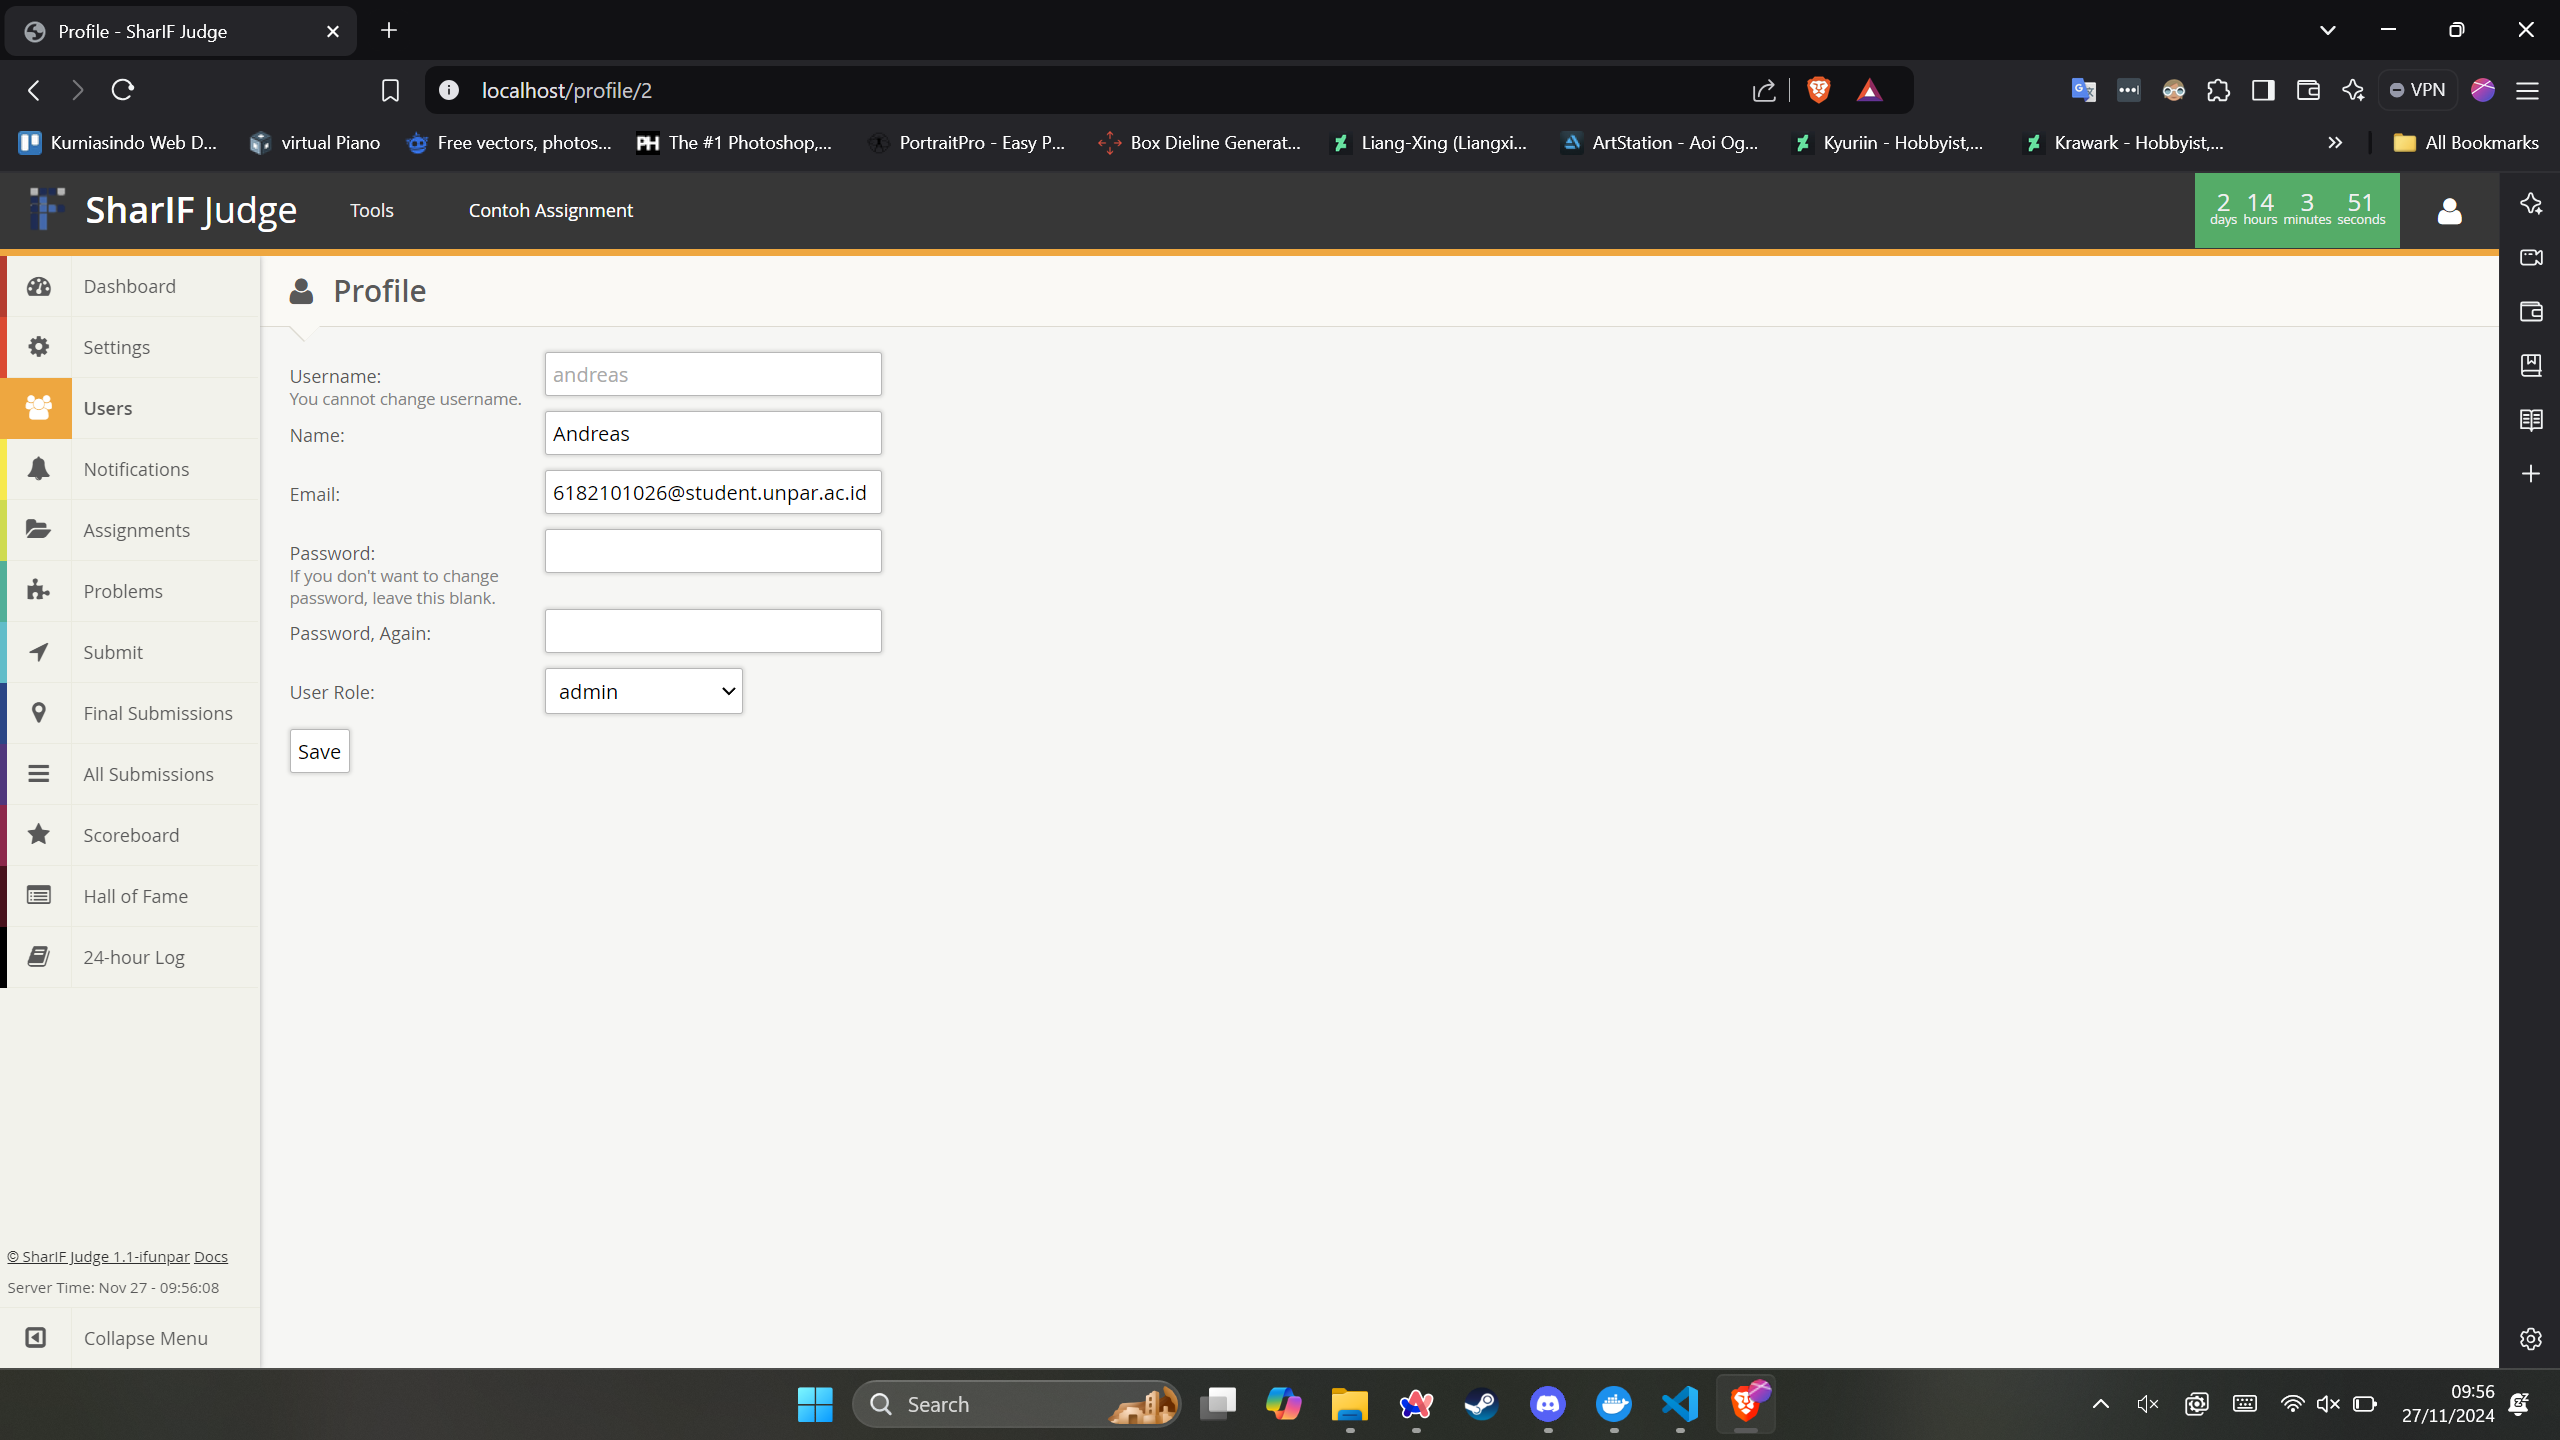
\includegraphics[width=\textwidth]{views/profile.png}
			            \caption{Halaman Profile}
			            \label{fig:3:1:1:profile}
		            \end{figure}

	      \end{itemize}

	\item \verb|Queue.php| \\
	      Berikut fungsi dengan penjelasannya pada \textit{controller} \verb|Profile.php|:

	      \begin{itemize}
		      \item \verb|pause()| \\
		            Memberhentikan proses \textit{queue}.
		      \item \verb|resume()| \\
		            Melanjutkan proses \textit{queue}.
		      \item \verb|empty_queue()| \\
		            Menghapus semua \textit{queue} yang ada.
		      \item \verb|index()| \\
		            Mendapatkan data dari \textit{model} \verb|Queue|, \verb|Assignments_model|, dan \verb|Settings_model| yang dipakai dalam \textit{view} \verb|queue.twig| dan ditampilkan kepada pengguna. Gambar \ref{fig:3:1:1:queue} menunjukkan hasil halaman Queue.

		            \begin{figure}[H]
			            \centering
			            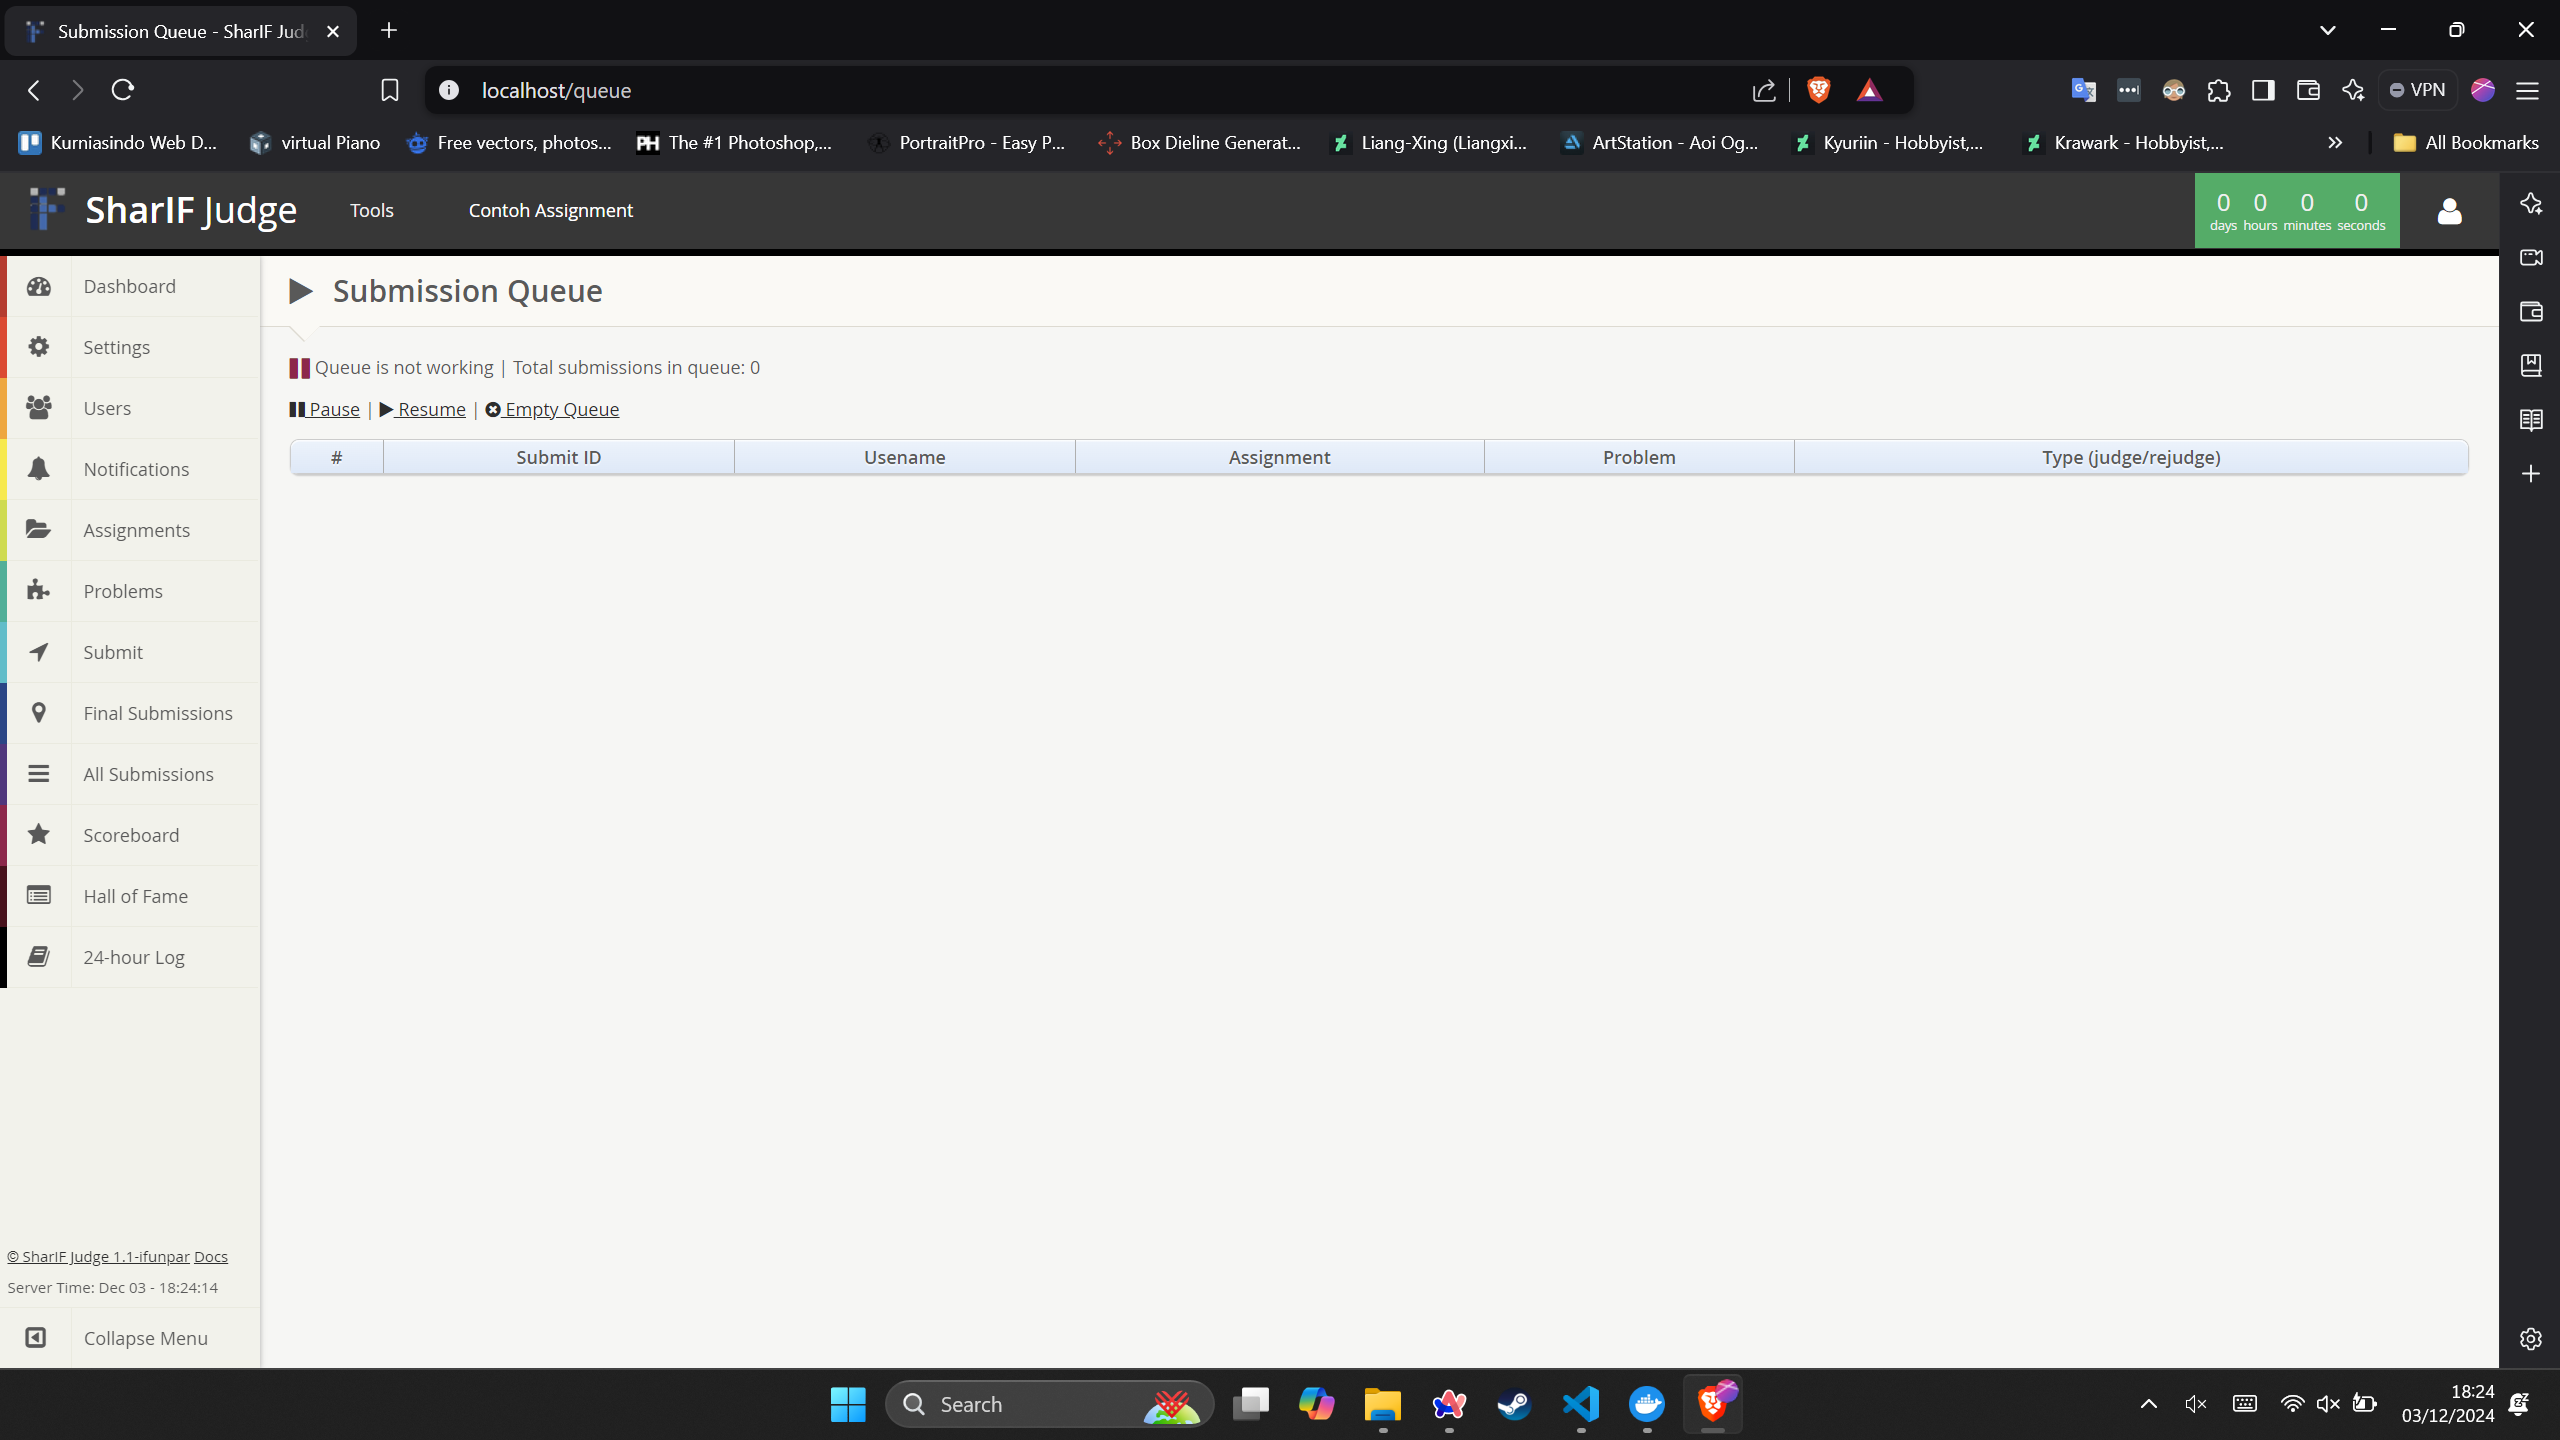
\includegraphics[width=\textwidth]{views/queue.png}
			            \caption{Halaman Queue}
			            \label{fig:3:1:1:queue}
		            \end{figure}

	      \end{itemize}

	\item \verb|Queueprocess.php| \\
	      \textit{Controller} \verb|Queueprocess.php| hanya memiliki satu fungsi yaitu \verb|run()| yang akan menjalankan \textit{queue} satu per satu menggunakan \verb|bash|.

	\item \verb|Rejudge.php| \\
	      Berikut fungsi dengan penjelasannya pada \textit{controller} \verb|Profile.php|:

	      \begin{itemize}
		      \item \verb|rejudge_single()| \\
		            Melakukan \textit{rejudge} untuk satu buah \textit{submission}.
		      \item \verb|index()| \\
		            Mendapatkan data dan menampilkan \textit{view} \verb|rejudge.twig|. Fungsi ini juga dapat melakukan \textit{rejudge} pada sebuah \textit{problem} tertentu. Gambar \ref{fig:3:1:1:rejudge} menunjukkan halaman Rejudge.

		            \begin{figure}[H]
			            \centering
			            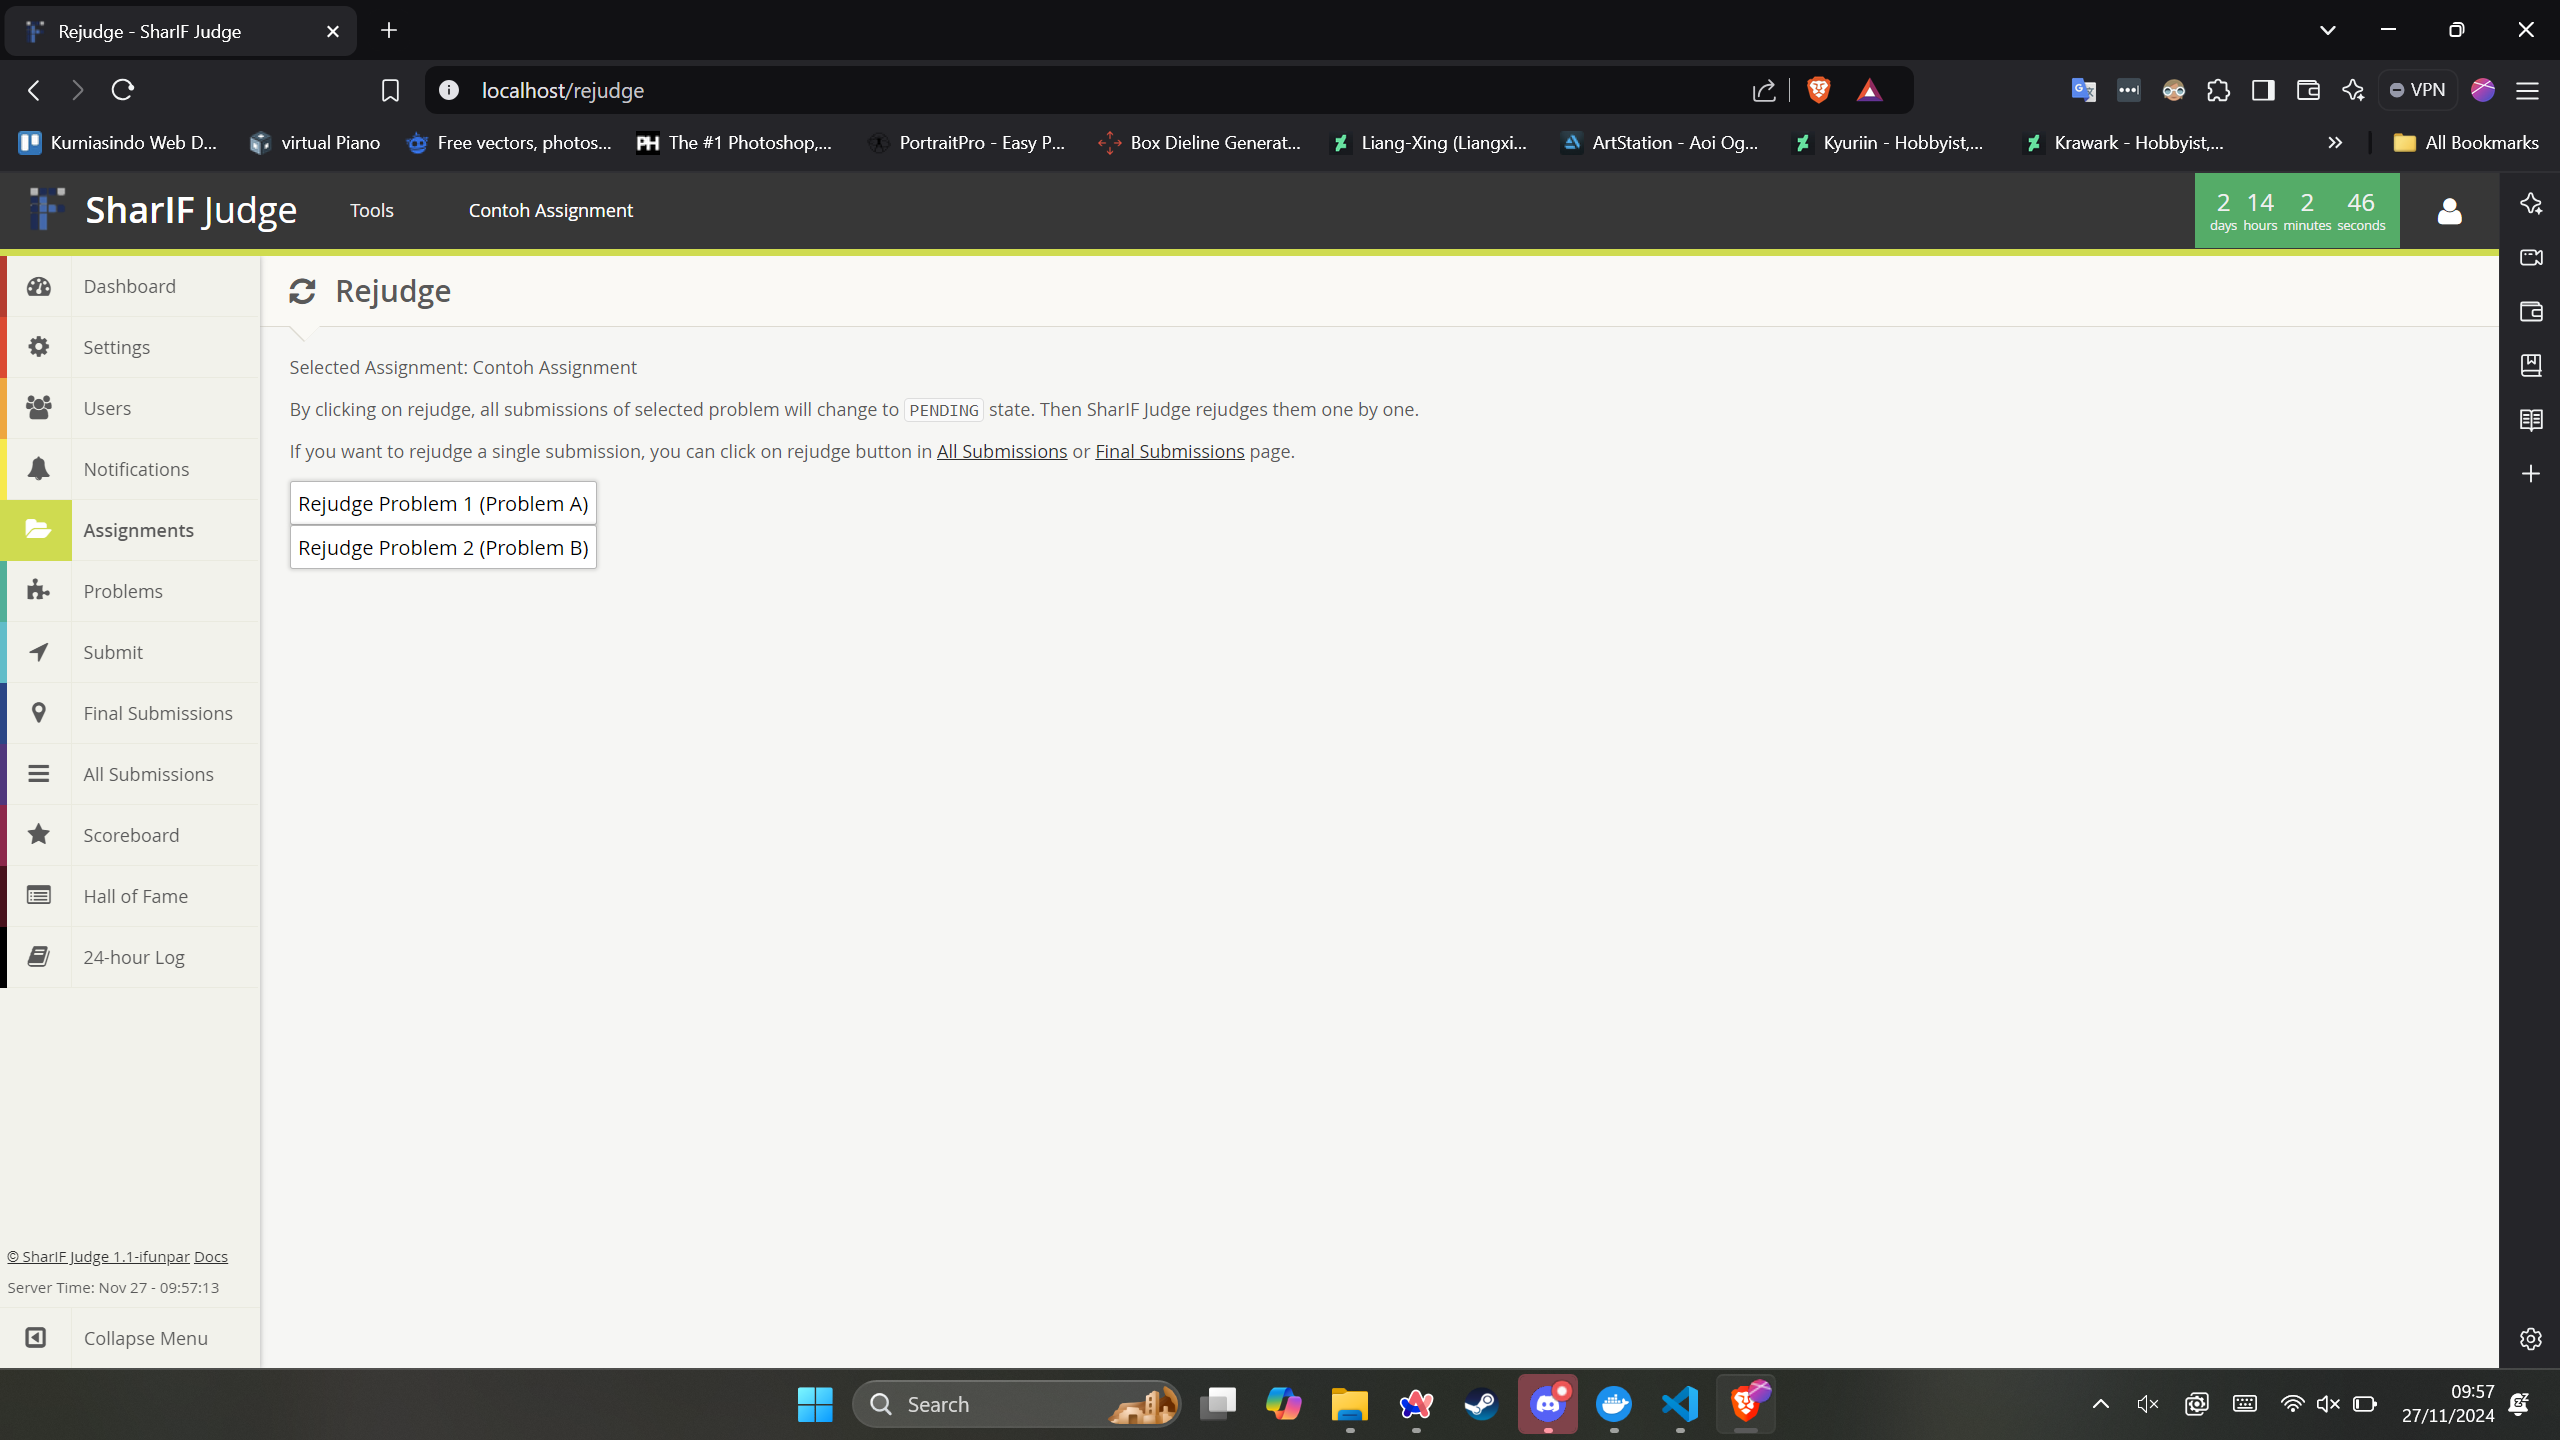
\includegraphics[width=\textwidth]{views/rejudge.png}
			            \caption{Halaman Rejudge}
			            \label{fig:3:1:1:rejudge}
		            \end{figure}

	      \end{itemize}

	\item \verb|Scoreboard.php| \\
	      \textit{Controller} \verb|Queueprocess.php| hanya memiliki satu fungsi yaitu \verb|index()| yang akan menampilkan \textit{view} \verb|scoreboard.twig| dengan data dari \verb|Scoreboard_model|. Gambar \ref{fig:3:1:1:scoreboard} menunjukkan hasil halaman Scoreboard.

	      \begin{figure}[H]
		      \centering
		      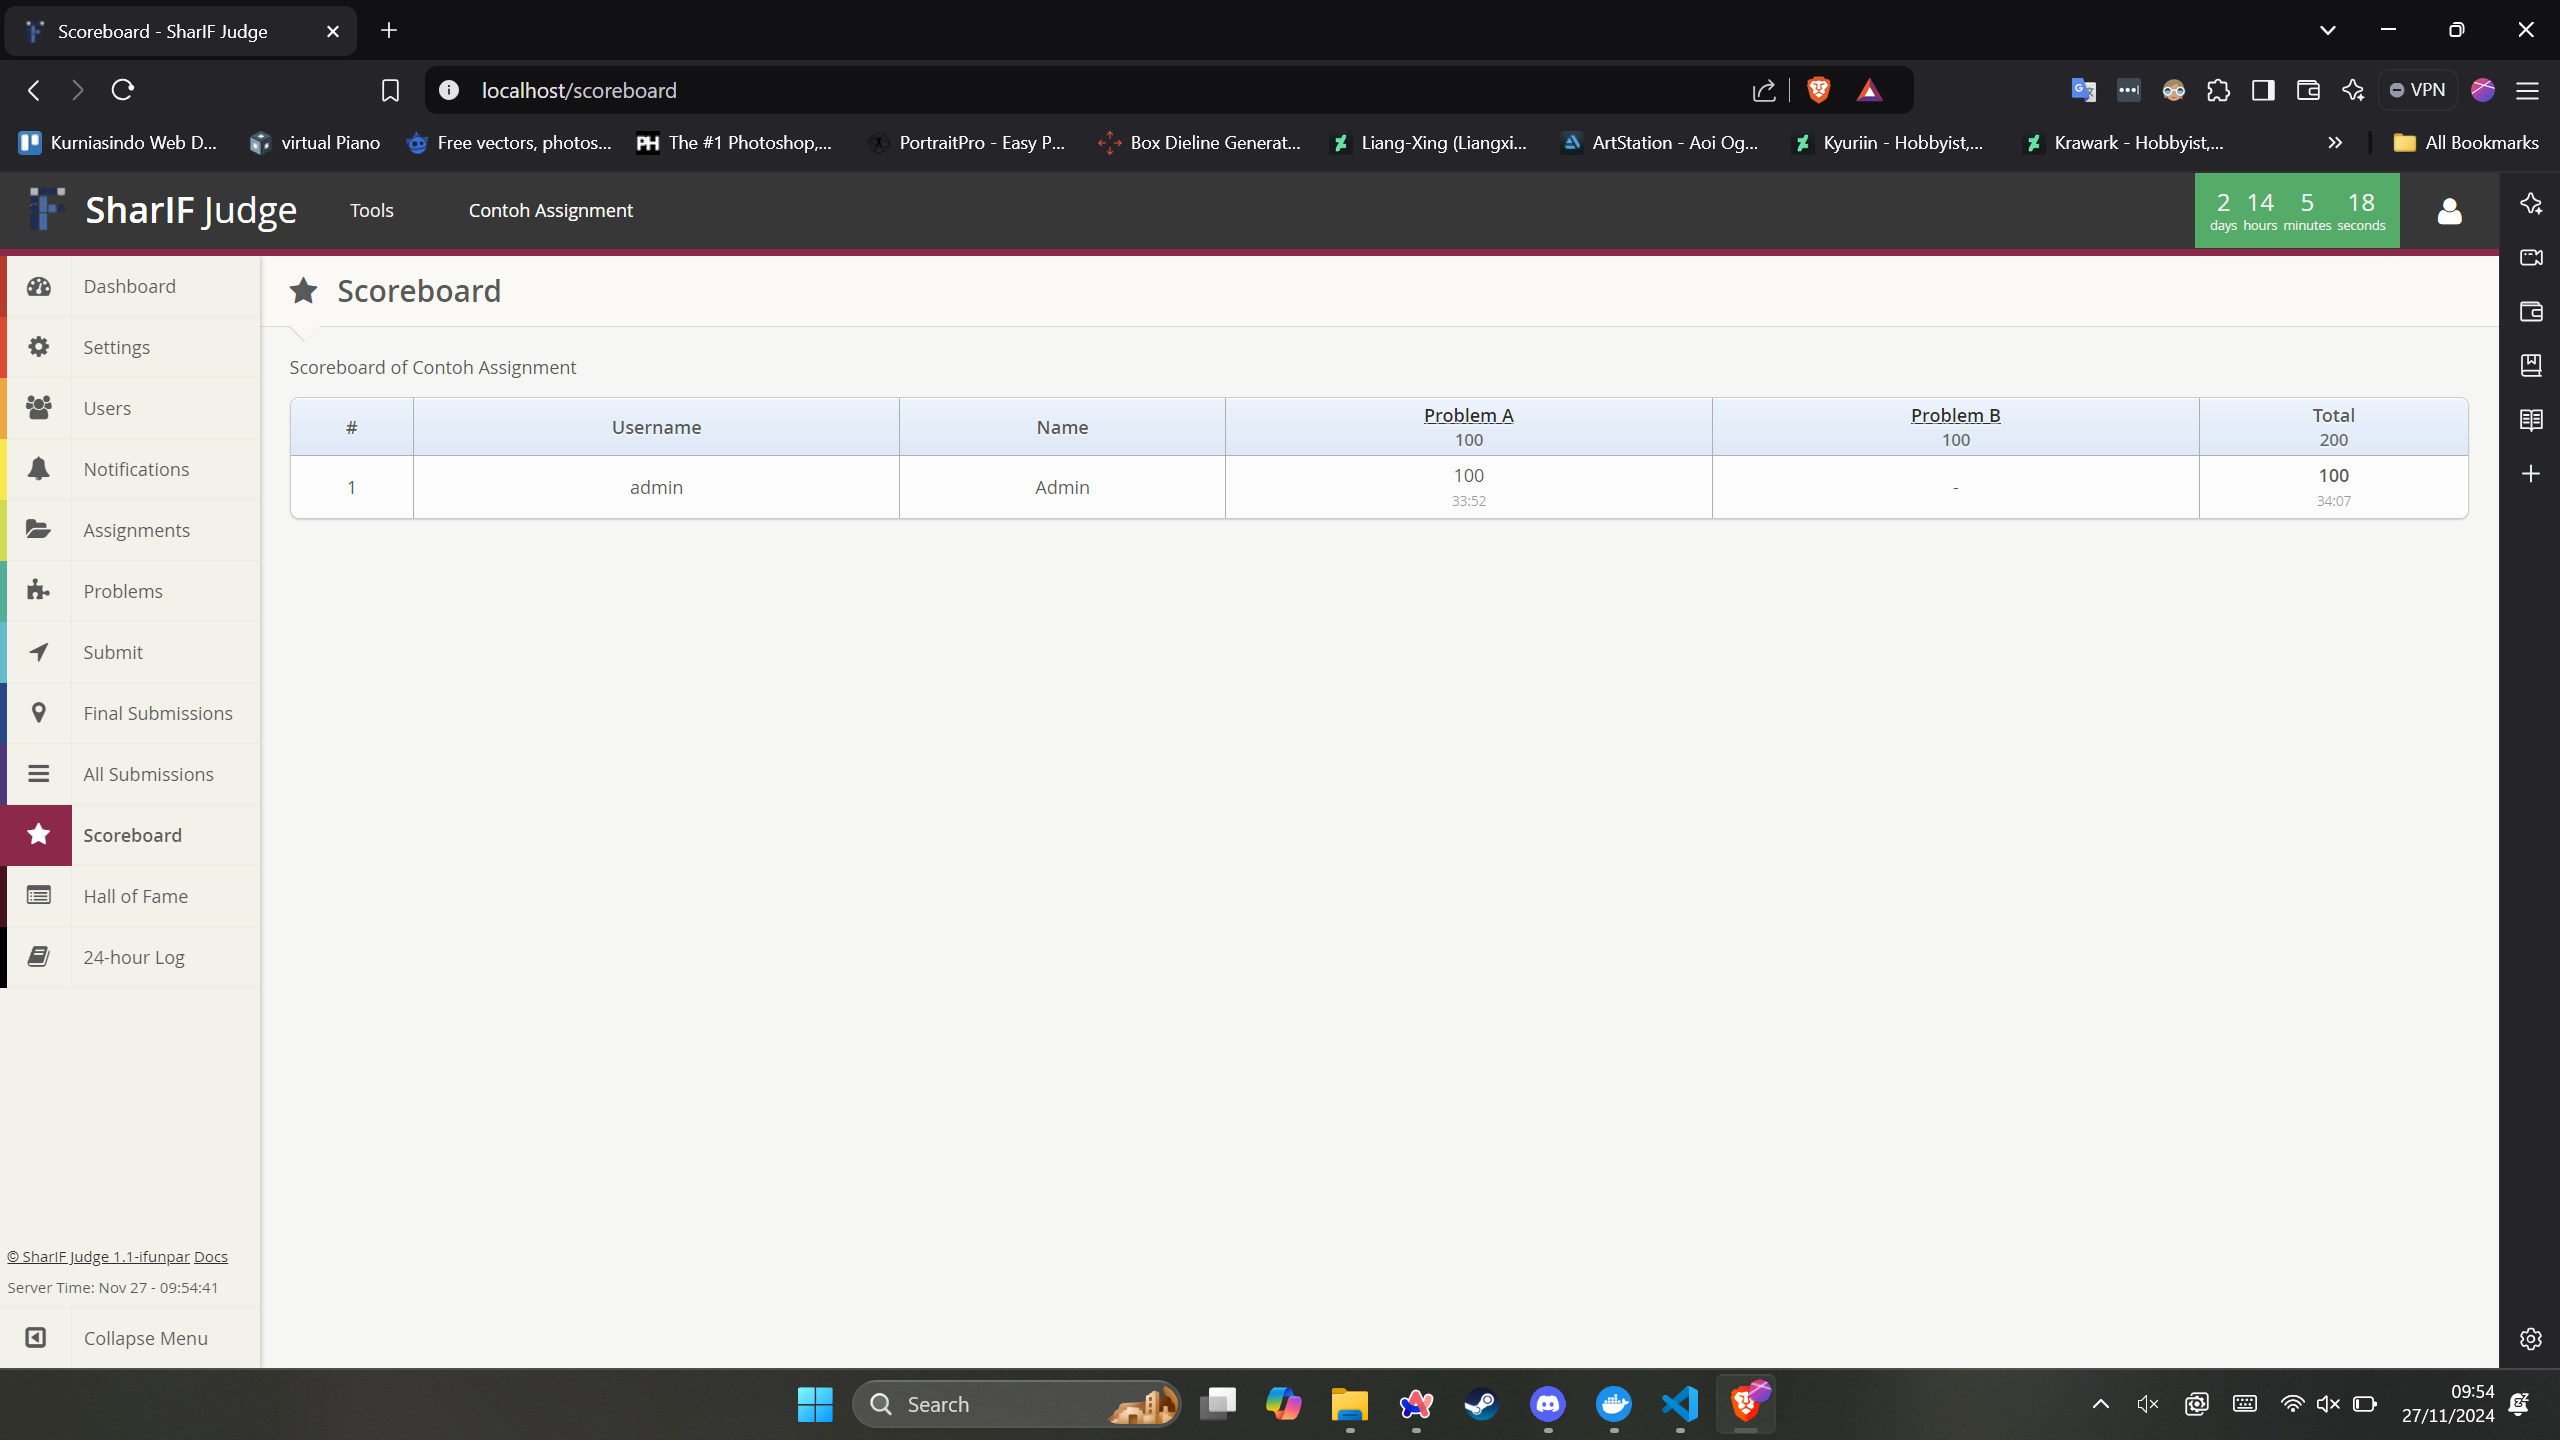
\includegraphics[width=\textwidth]{views/scoreboard.png}
		      \caption{Halaman Scoreboard}
		      \label{fig:3:1:1:scoreboard}
	      \end{figure}

	\item \verb|Server_time.php| \\
	      \textit{Controller} \verb|Queueprocess.php| hanya memiliki satu fungsi yaitu \verb|index()| yang akan mencetak waktu pada \textit{server}, waktu akan digunakan untuk sinkronisasi waktu.

	\item \verb|Settings.php| \\
	      Berikut fungsi dengan penjelasannya pada \textit{controller} \verb|Settings.php|:

	      \begin{itemize}
		      \item \verb|update()| \\
		            Memperbaharui \textit{settings} dari masukkan pengguna.
		      \item \verb|index()| \\
		            Mendapatkan data dari \verb|Settings_model| dan menampilkan \textit{view} \verb|settings.twig|. Jika terdapat \textit{error setting} pada sistem, akan ditampilkan juga pada \textit{view} tersebut. Gambar \ref{fig:3:1:1:settings} menunjukkan hasil halaman Users.

		            \begin{figure}[H]
			            \centering
			            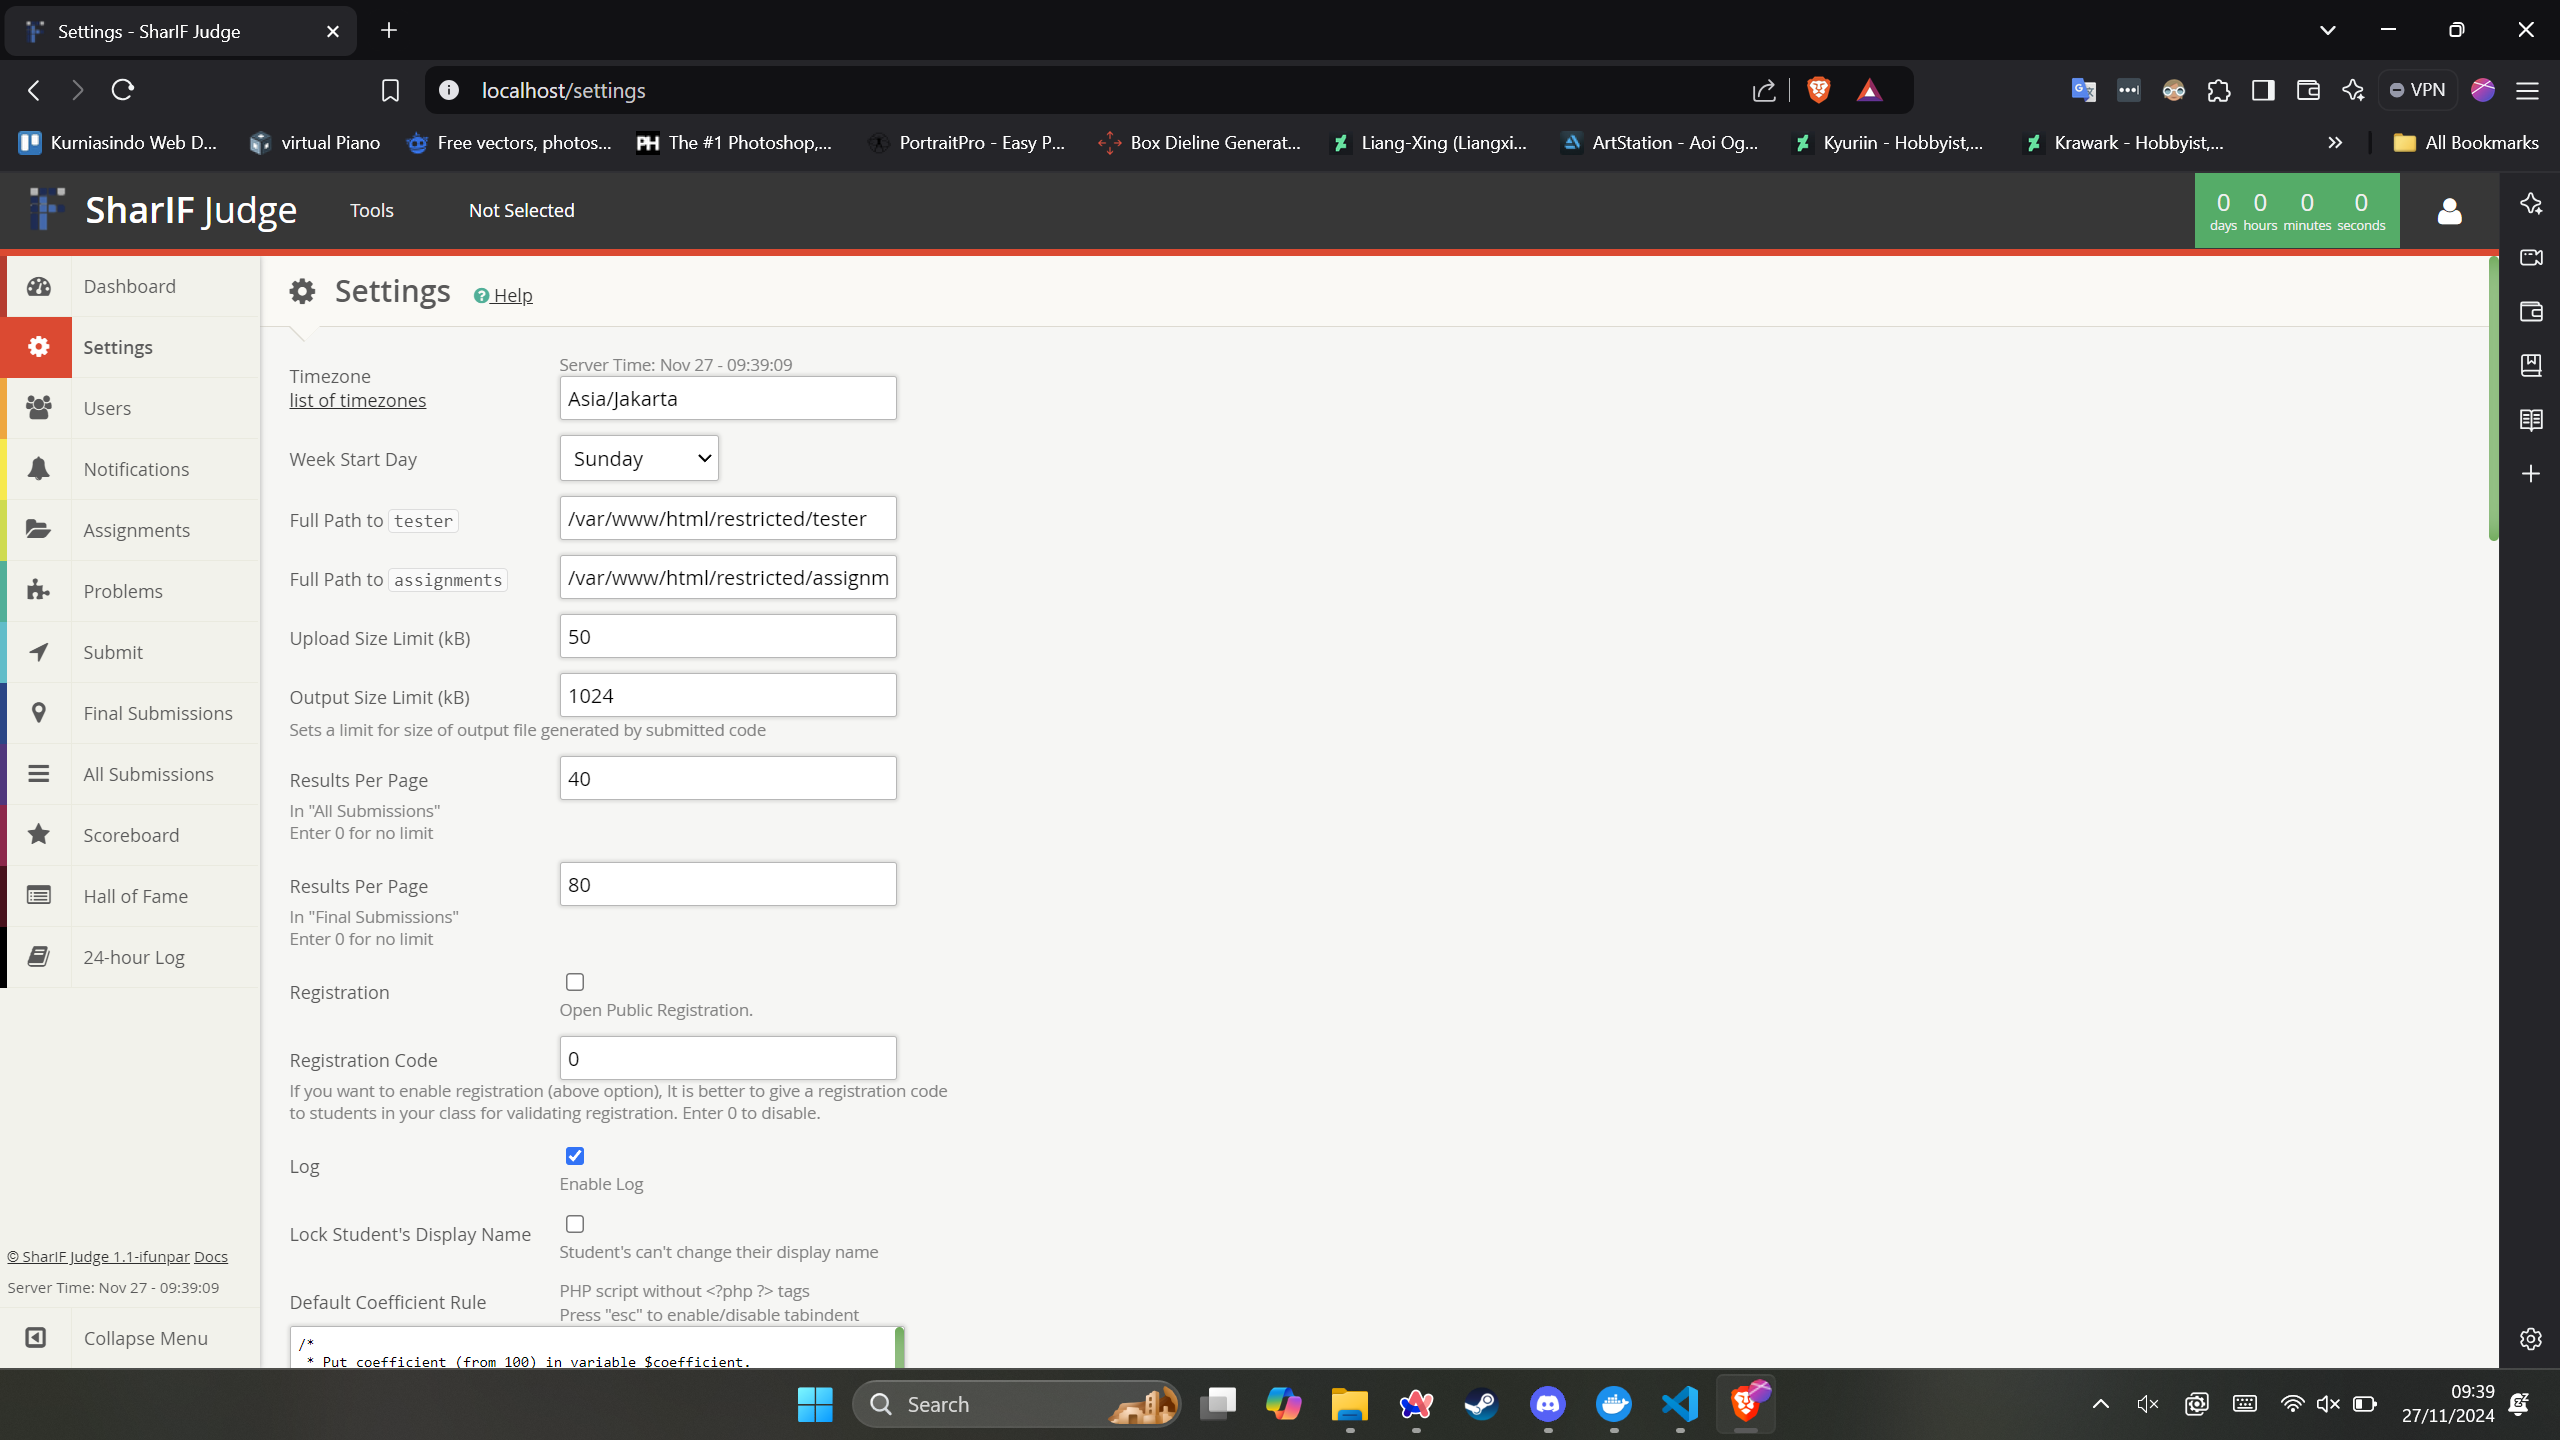
\includegraphics[width=\textwidth]{views/settings.png}
			            \caption{Halaman Settings}
			            \label{fig:3:1:1:settings}
		            \end{figure}

	      \end{itemize}

	\item \verb|Submissions.php| \\
	      Berikut fungsi dengan penjelasannya pada \textit{controller} \verb|Submissions.php|:

	      \begin{itemize}
		      \item \verb|_download_excel($view)| \\
		            Menggunakan \textit{library} PHPExcel untuk membuat sebuah \textit{file excel} dari \textit{submissions} yang akan diunduh pengguna.
		      \item \verb|final_excel()| \\
		            Menggunakan fungsi \verb|_download_excel| untuk mendownload \textit{final submission}.
		      \item \verb|all_excel()| \\
		            Menggunakan fungsi \verb|_download_excel| untuk mendownload seluruh \textit{submission}.
		      \item \verb|select()| \\
		            Menggunakan \textit{ajax request} untuk memilih \textit{submission} yang akan dikumpulkan atau menjadi \textit{final}.
		      \item \verb|_check_type($type)| \\
		            Melakukan validasi tipe \textit{submission} yang dikumpulkan.
		      \item \verb|view_code()| \\
		            Digunakan untuk melihat kode, melihat hasil kode, atau melihat \textit{log} sebuah \textit{submission}.
		      \item \verb|download_file()| \\
		            Mengunduh \textit{file} kode sebuah \textit{submission}.
		      \item \verb|the_final()| \\
		            Mendapatkan data dari \verb|Submit_model| untuk mendapatkan \textit{final submission} dan menampilkan halaman \verb|submission.twig| berisi \textit{final submission}. Gambar \ref{fig:3:1:1:final} menunjukkan halaman Final Submissions .
		            \begin{figure}[H]
			            \centering
			            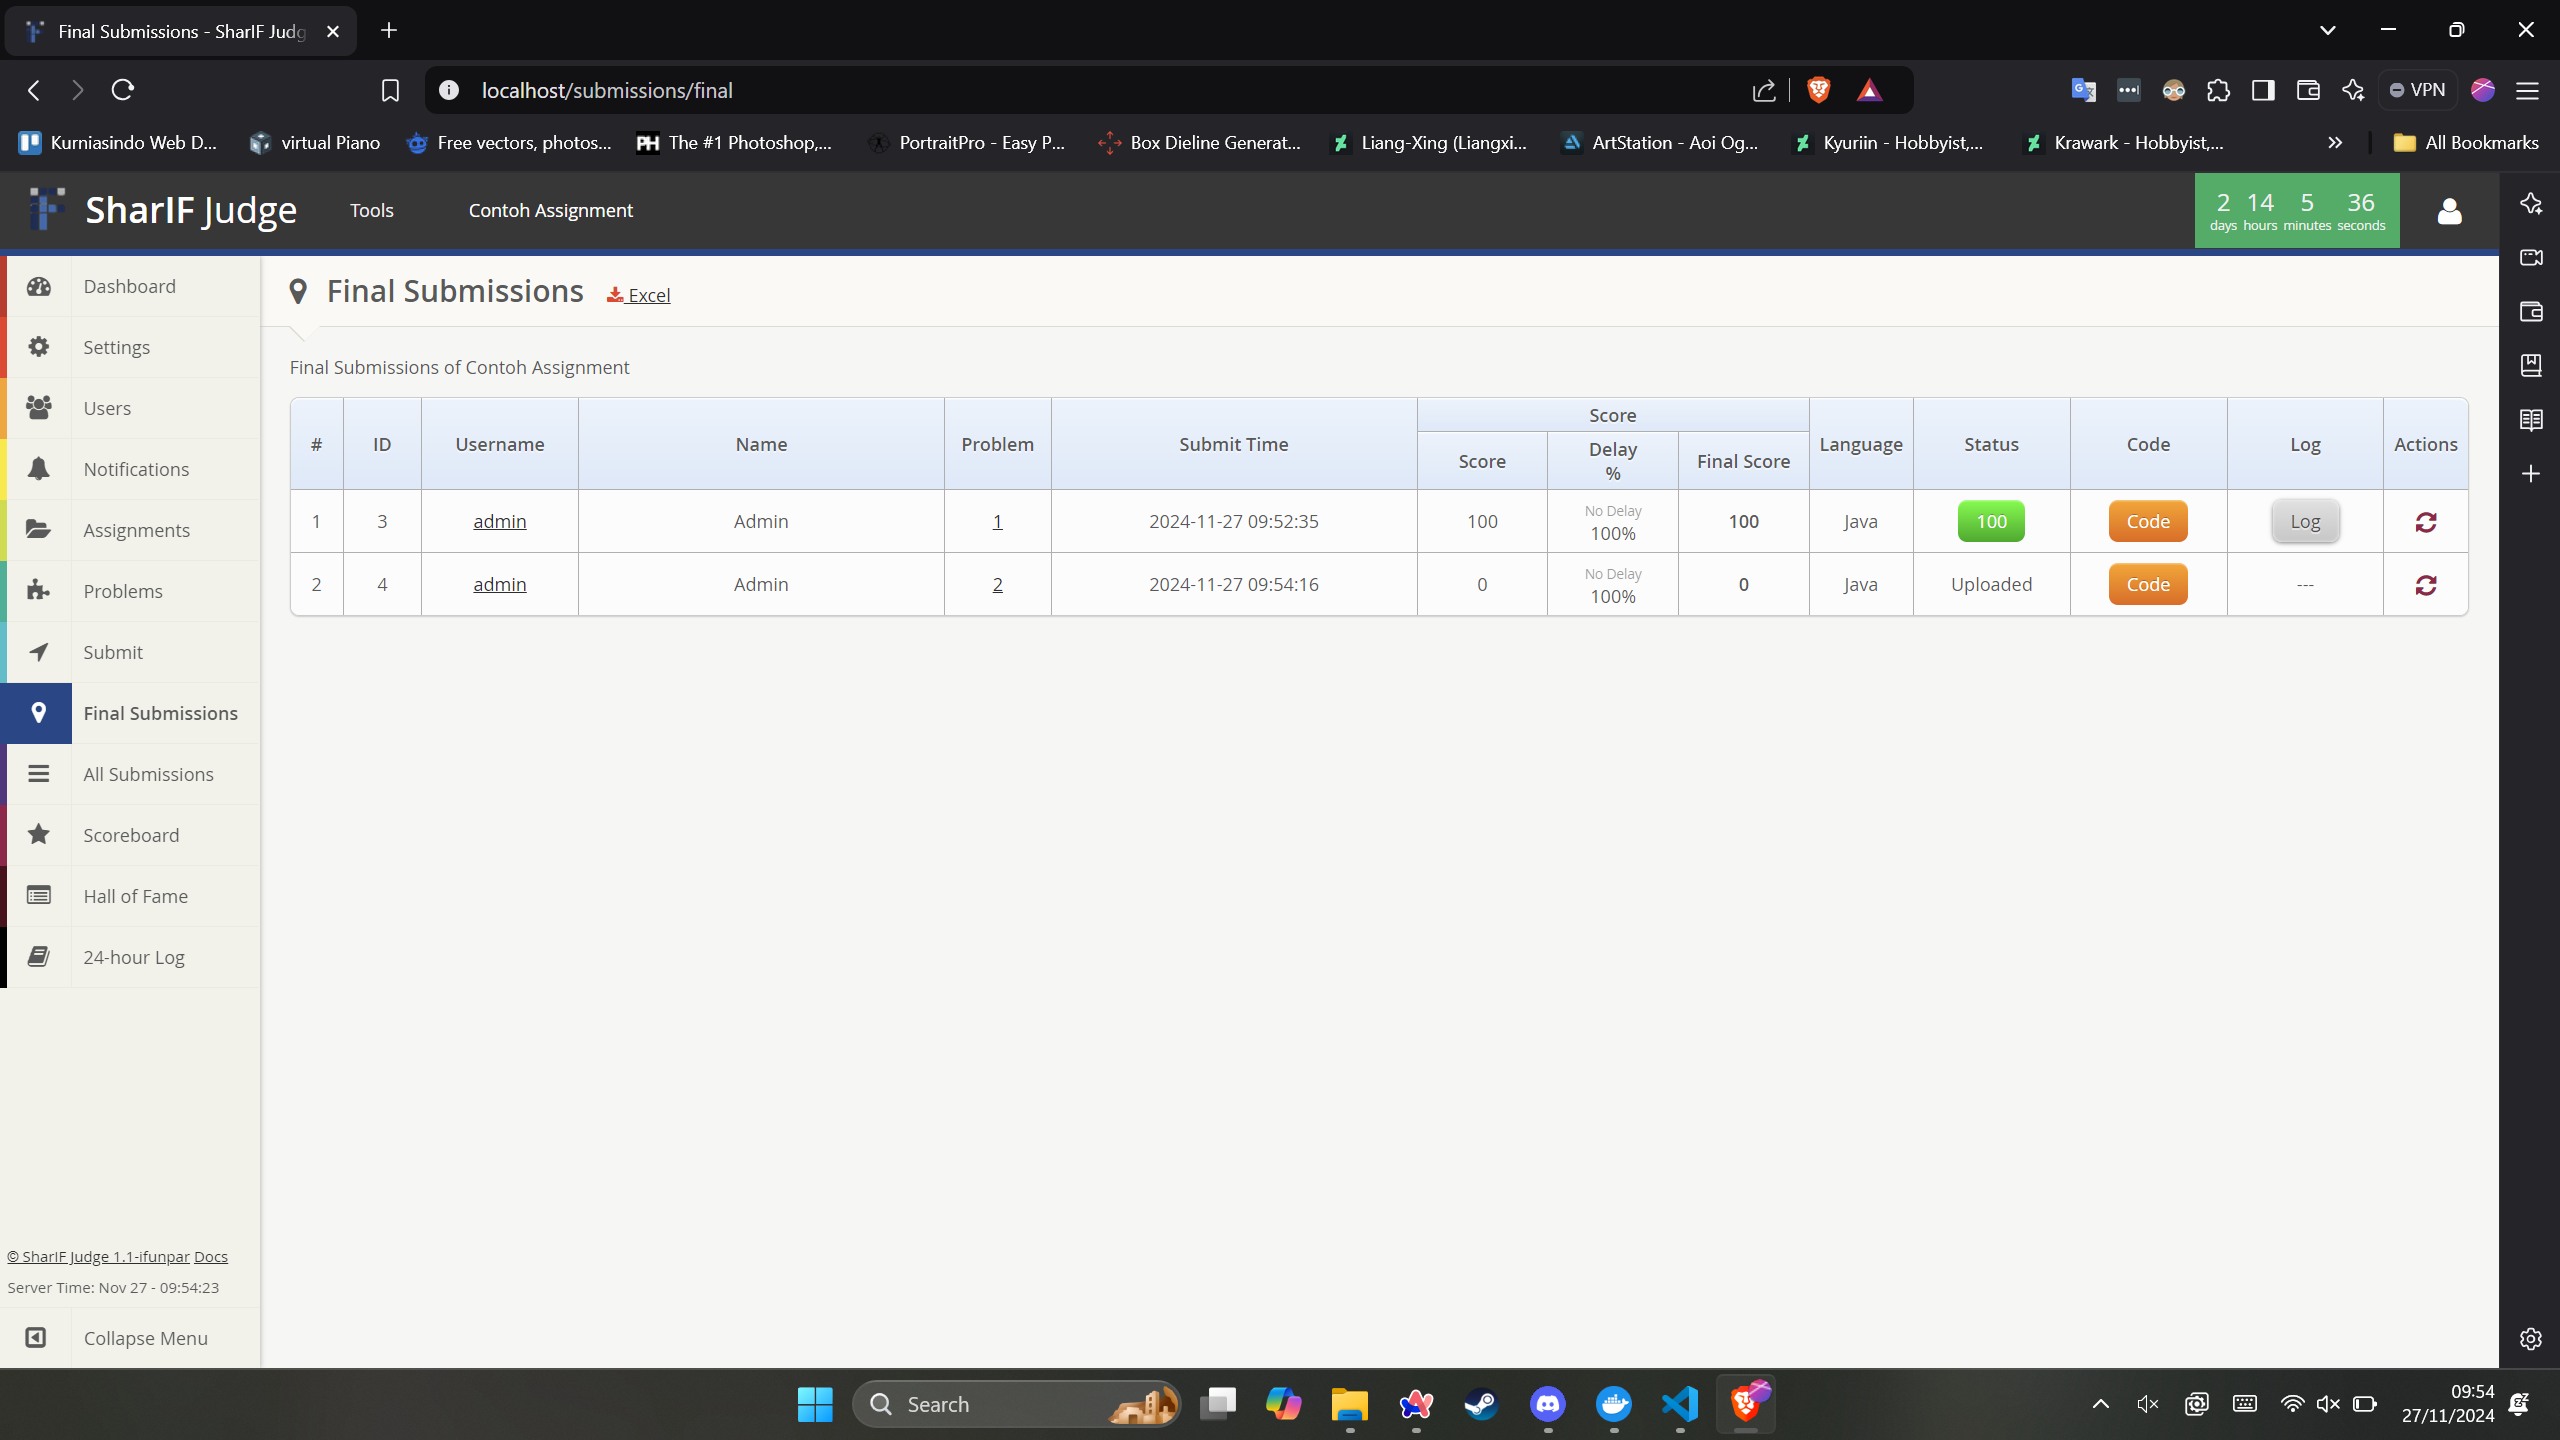
\includegraphics[width=\textwidth]{views/final_submissions.png}
			            \caption{Halaman Final Submissions}
			            \label{fig:3:1:1:final}
		            \end{figure}

		      \item \verb|all()| \\
		            Mendapatkan data dari \verb|Submit_model| untuk mendapatkan seluruh \textit{submission} dan menampilkan halaman \verb|submission.twig| berisi semua \textit{submission}. Gambar \ref{fig:3:1:1:all} menunjukkan halaman All Submissions .

		            \begin{figure}[H]
			            \centering
			            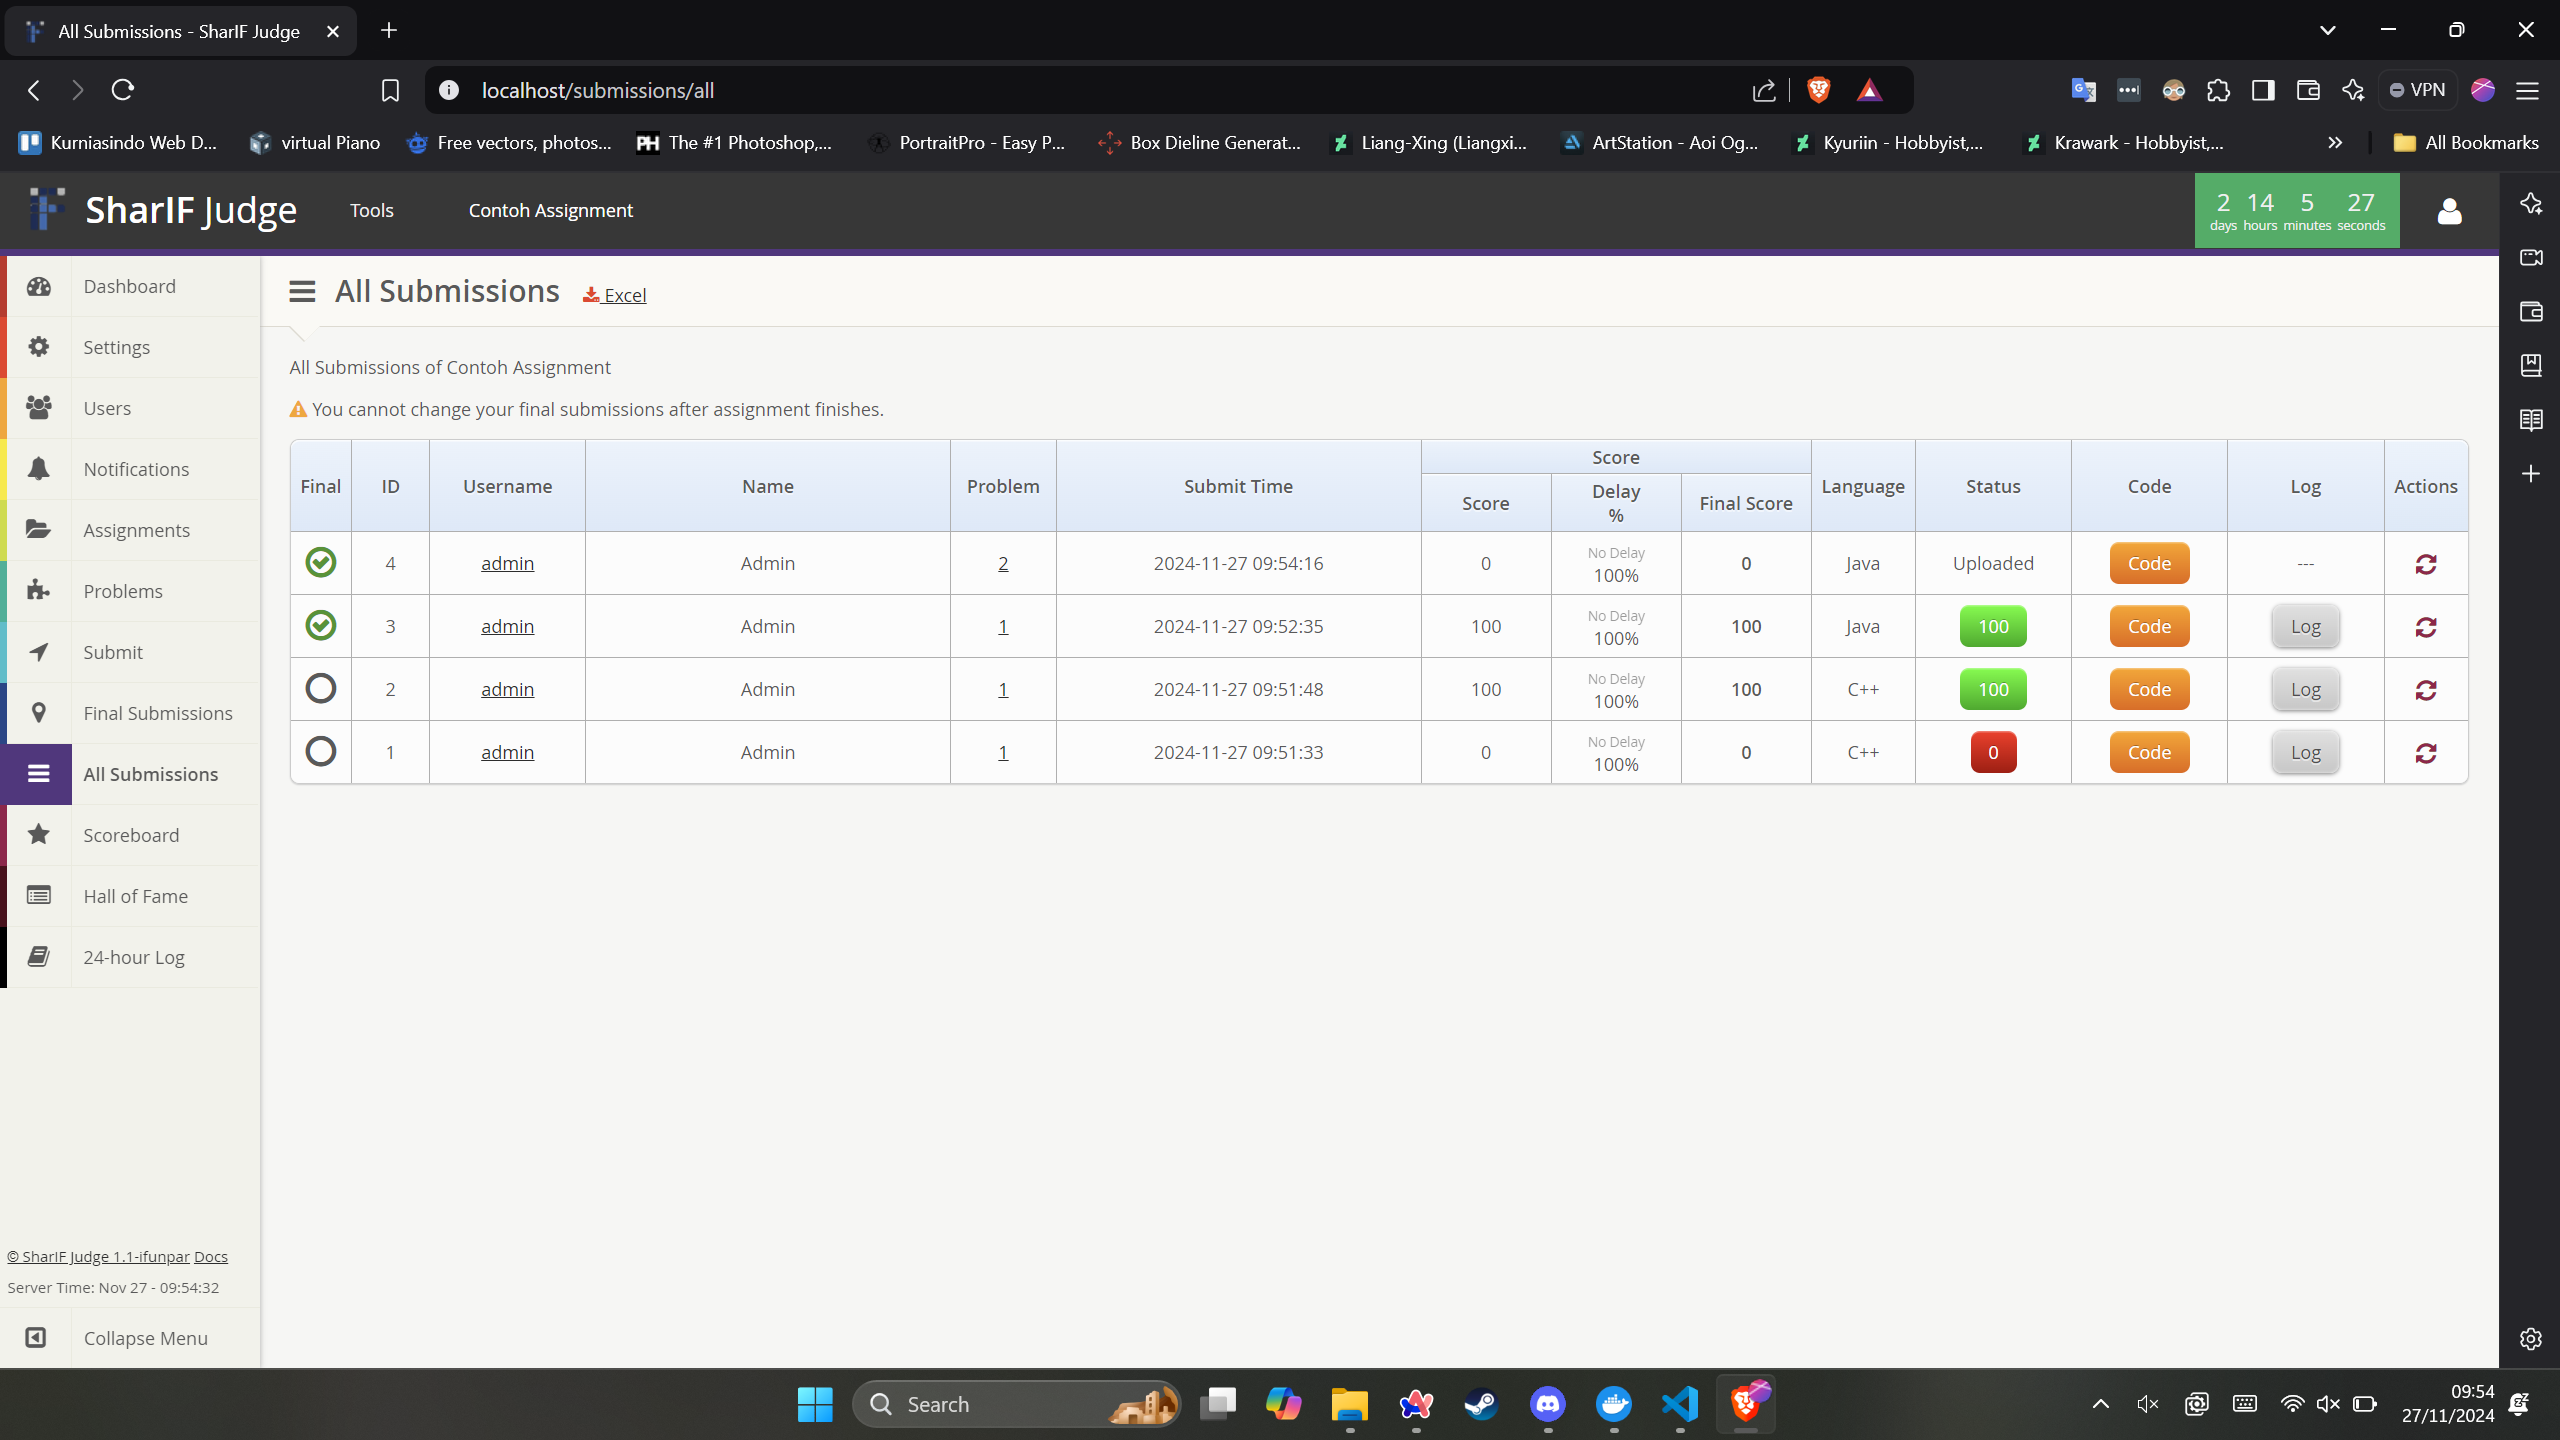
\includegraphics[width=\textwidth]{views/all_submissions.png}
			            \caption{Halaman All Submissions}
			            \label{fig:3:1:1:all}
		            \end{figure}
	      \end{itemize}

	\item \verb|Submit.php| \\
	      Berikut fungsi dengan penjelasannya pada \textit{controller} \verb|Submit.php|:

	      \begin{itemize}
		      \item \verb|_language_to_type($language)| \\
		            Mengembalikan kode singkat dari \verb|$language| dipilih.
		      \item \verb|_language_to_ext($language)| \\
		            Mengembalikan extensi file dari \verb|$language| yang dipilih.
		      \item \verb|_match($type, $extension)| \\
		            Melakukan validasi untuk \verb|$type| dan \verb|$extension| agar sesuai.
		      \item \verb|_check_language($str)| \\
		            Melakukan validasi sudah dipilihannya bahasa.
		      \item \verb|_upload()| \\
		            Menyimpan jawaban pengguna yang dikirim dan menambahkannya ke dalam \textit{queue} untuk dinilai jika bukan \textit{upload only problem}.
		      \item \verb|load($problem_id)| \\
		            Mendapatkan isi file dan menaruh isi file ke editor kode.
		      \item \verb|save($type)| \\
		            Menyimpan isi editor kode ke dalam \textit{server} dan menjalankan atau mengumpulkan jika diinginkan.
		      \item \verb|_submit($data, $problem_id, $language, $user_dir)| \\
		            Menambahkan kode ke dalam \textit{submission} untuk dinilai.
		      \item \verb|_execute($data, $problem_id, $language, $user_dir)| \\
		            Menambahkan kode ke dalam \textit{queue} untuk di jalankan saja.
		      \item \verb|get_output($problem_id)| \\
		            Mendapatkan keluaran dari kode yang telah dijalankan sebagai hasil eksekusi.
		      \item \verb|index()| \\
		            Mendapatkan data dari \textit{model} \verb|Assignments_model| untuk mendapatkan \textit{problem} dan data lainnya. Semua data akan dimasukkan dalam \textit{view} \verb|submit.twig|. Gambar \ref{fig:3:1:1:submit} menunjukkan hasil halaman Submit. Halaman ini terdapat editor kode yang sudah di implementasikan~\cite{nicholas:sharif}.

		            \begin{figure}[H]
			            \centering
			            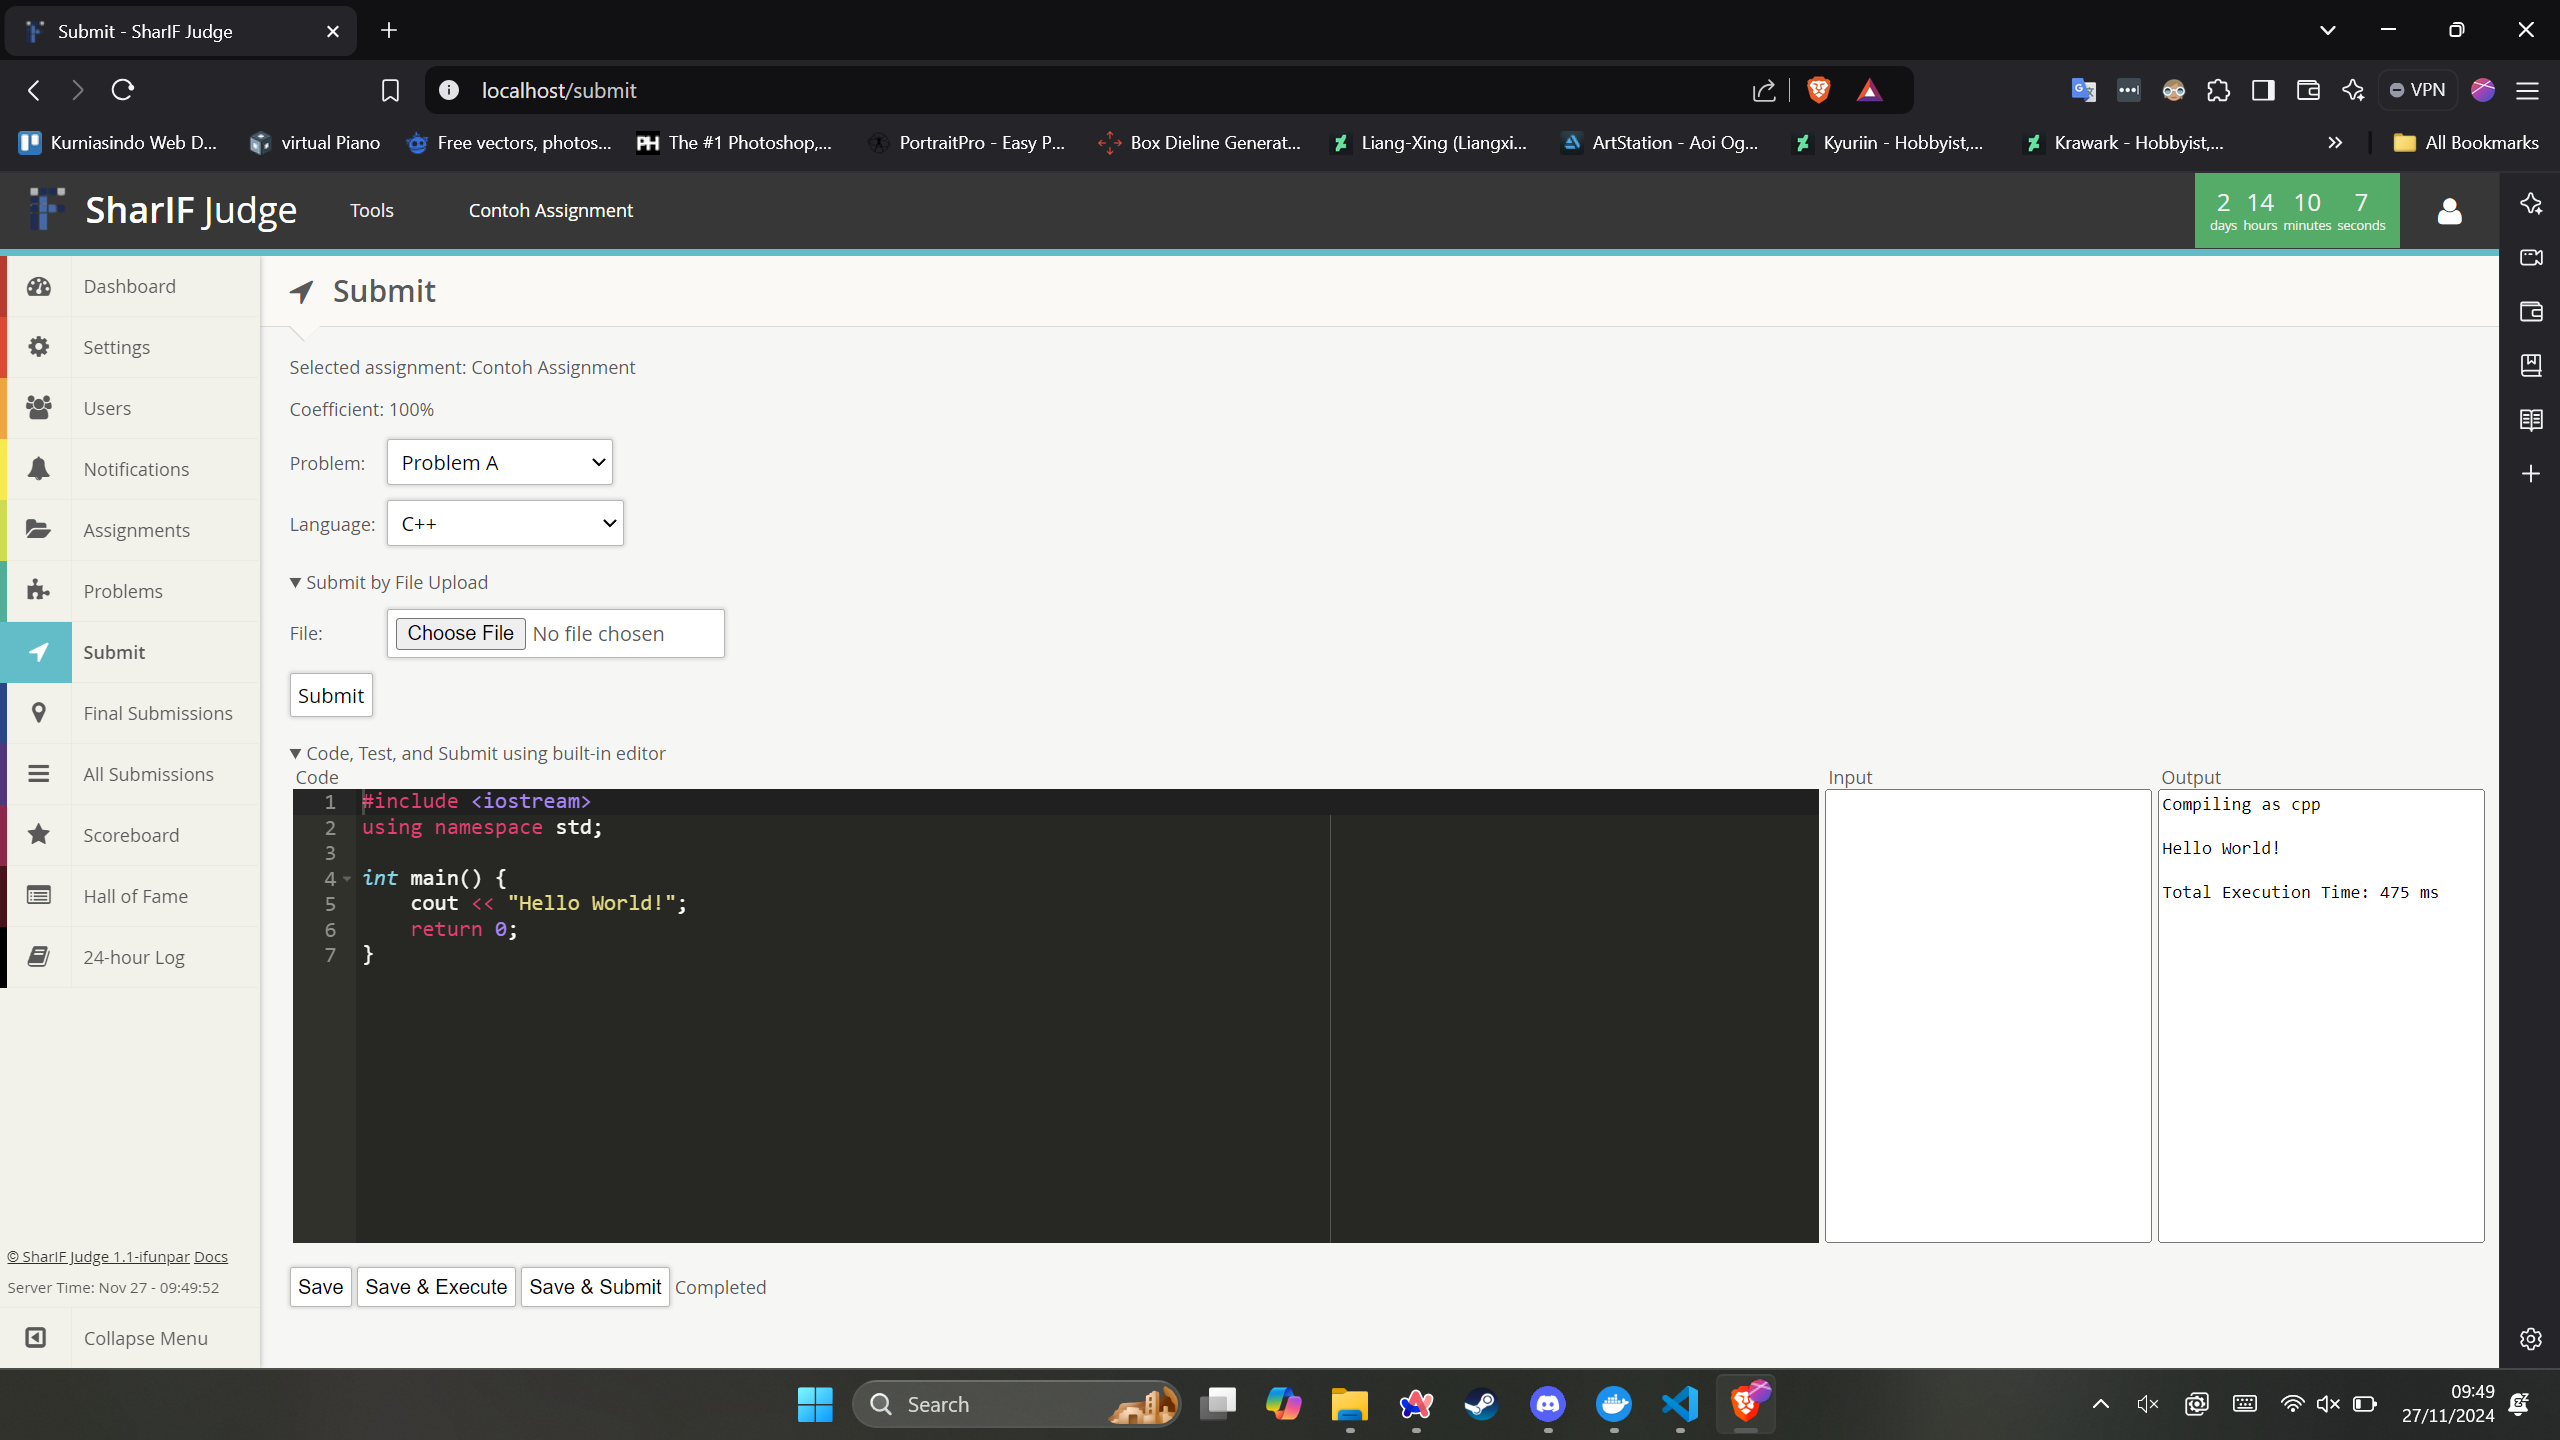
\includegraphics[width=\textwidth]{views/submit.png}
			            \caption{Halaman Submit}
			            \label{fig:3:1:1:submit}
		            \end{figure}

	      \end{itemize}

	\item \verb|User.php| \\
	      Berikut fungsi dengan penjelasannya pada \textit{controller} \verb|User.php|:

	      \begin{itemize}
		      \item \verb|add()| \\
		            Menambahkan \textit{user} baru ke dalam \textit{sistem}.
		      \item \verb|delete()| \\
		            Menghapus sebuah \textit{user}.
		      \item \verb|delete_submissions()| \\
		            Menghapus seluruh \textit{submissions} dari sebuah \textit{user}.
		      \item \verb|list_excel()| \\
		            Menggunakan \textit{library} PHPExcel untuk membuat sebuah file excel dari seluruh daftar \textit{user} yang akan diunduh pengguna.
		      \item \verb|index()| \\
		            Mendapatkan data dari \verb|User_model| dan menunjukkan \textit{view} \verb|users.twig|. Gambar \ref{fig:3:1:1:users} menunjukkan hasil halaman Users. Pada halaman ini terdapat daftar seluruh \textit{user} yang terdaftar pada SharIF Judge. Pengguna dapat membuat, memperbaharui, dan menghapus \textit{user}.

		            \begin{figure}[H]
			            \centering
			            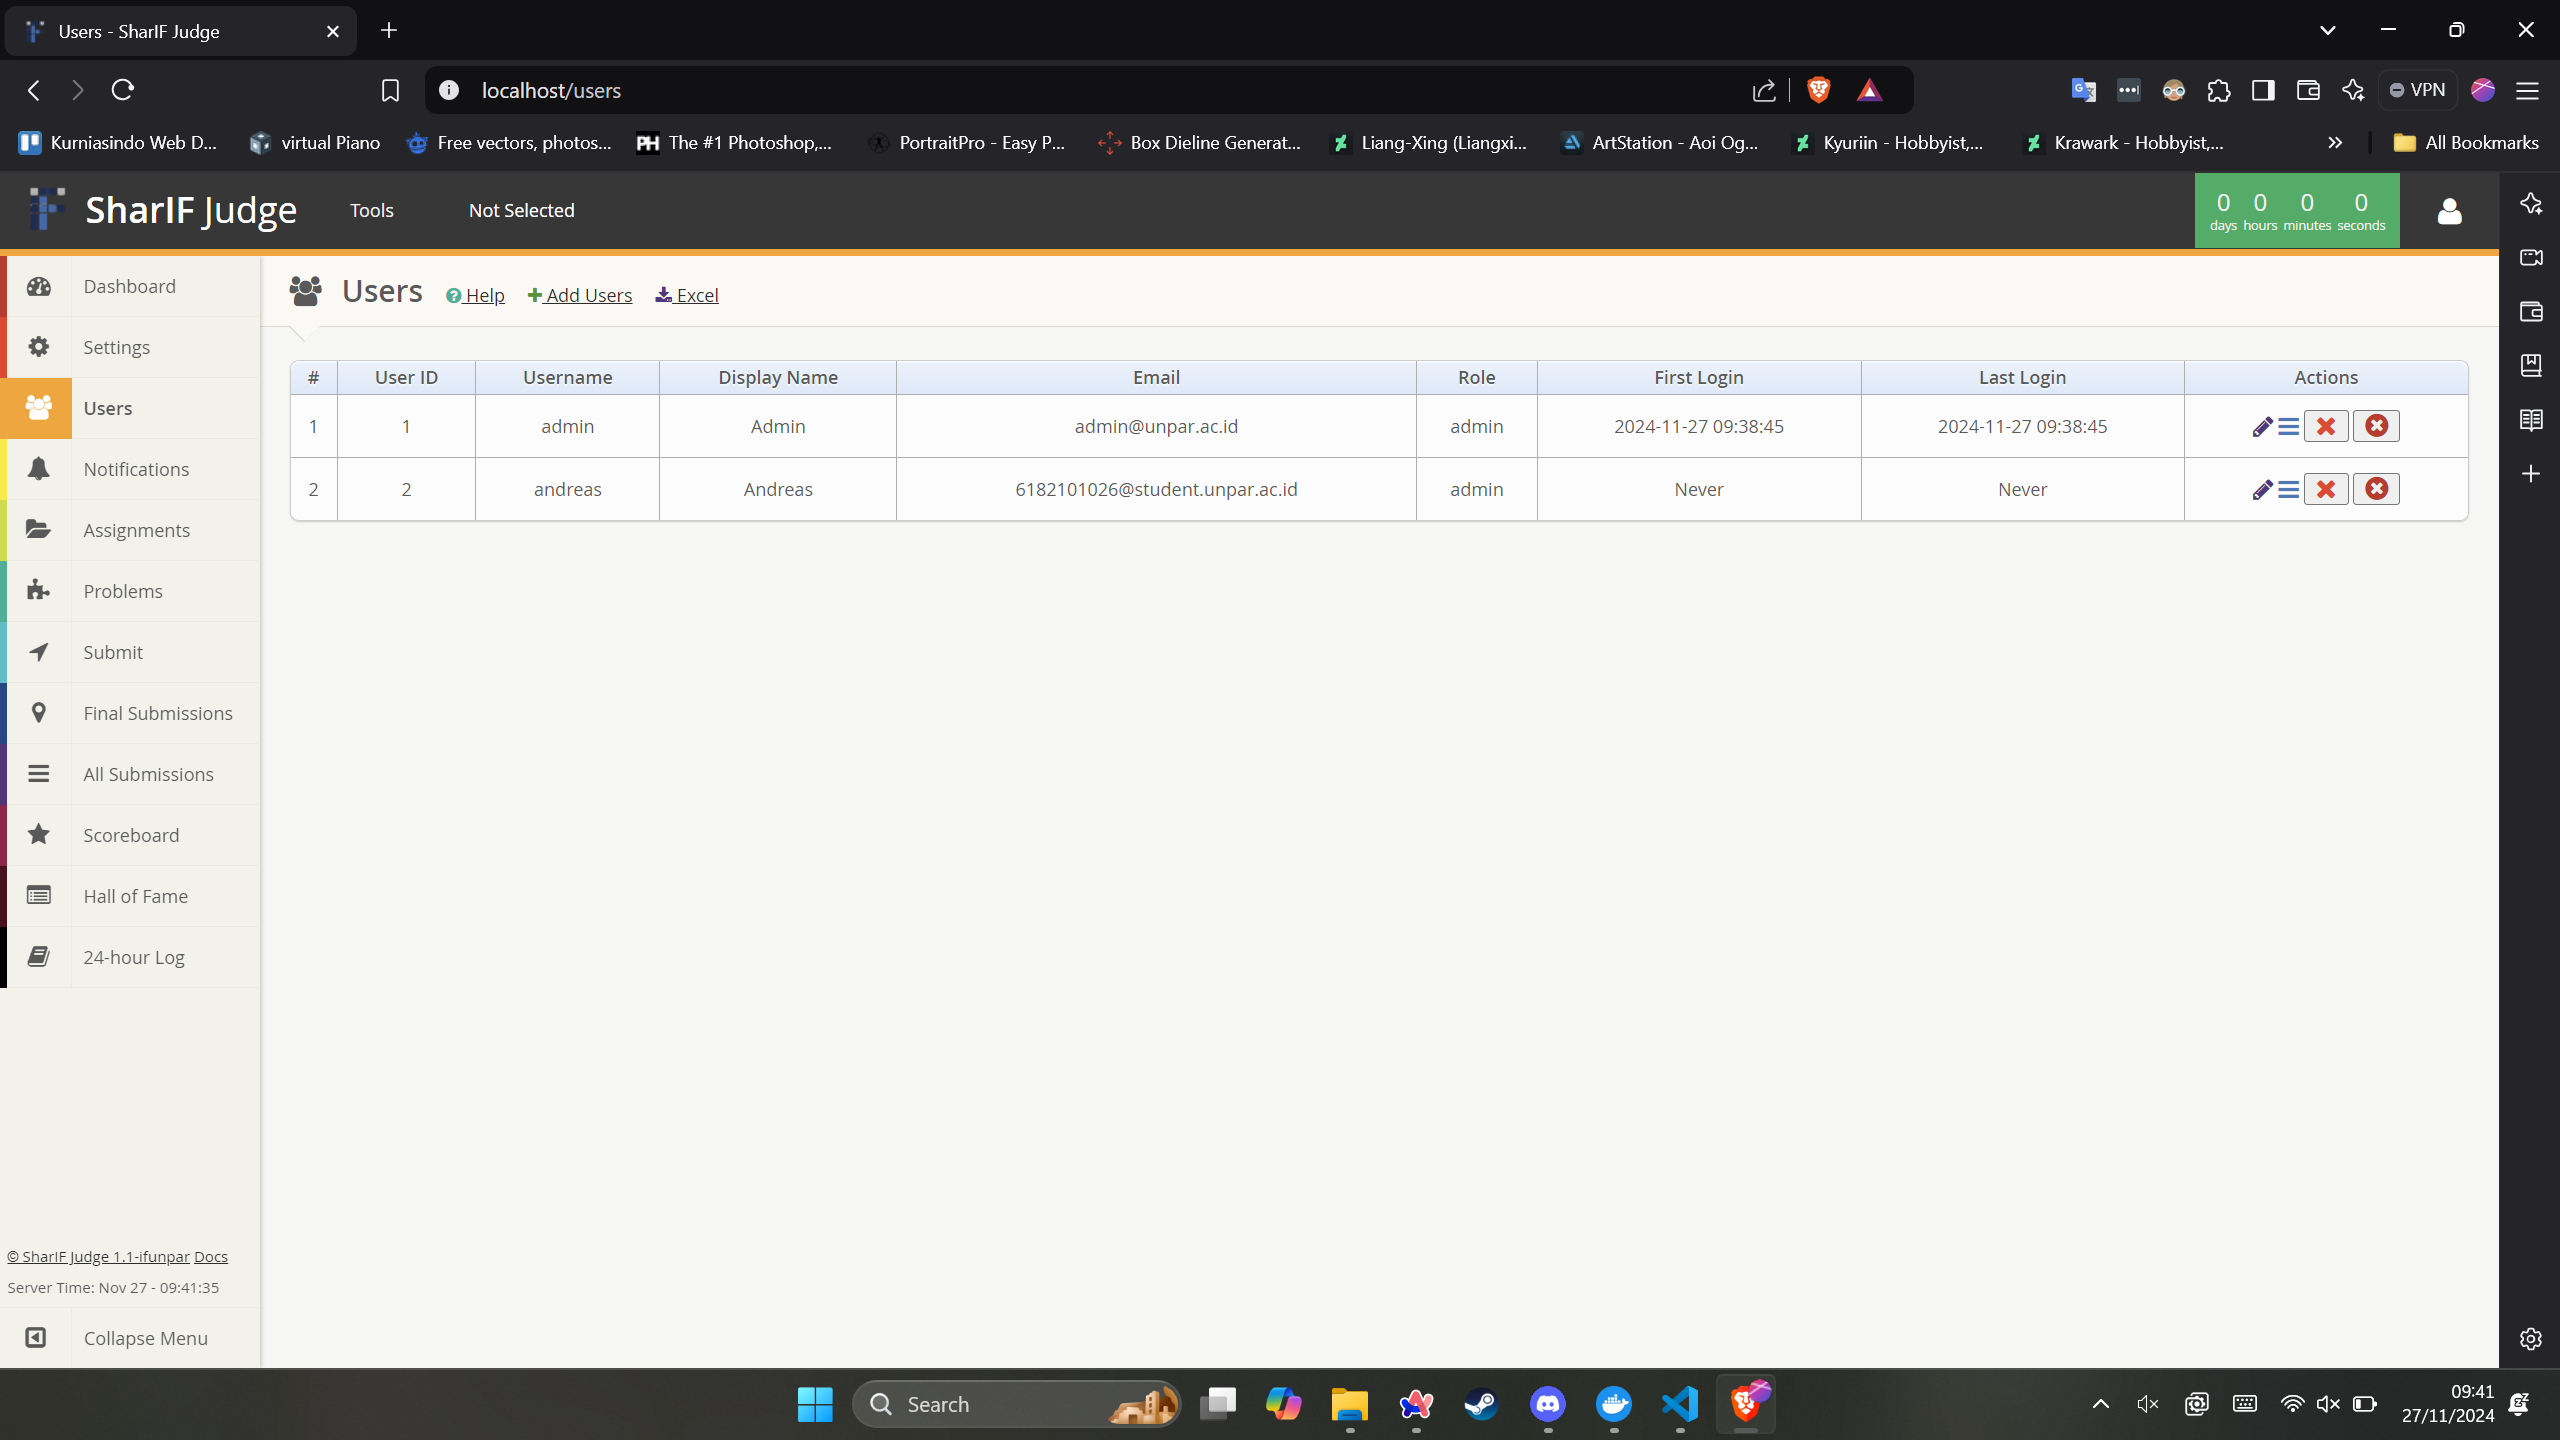
\includegraphics[width=\textwidth]{views/users.png}
			            \caption{Halaman Users}
			            \label{fig:3:1:1:users}
		            \end{figure}


	      \end{itemize}

\end{itemize}

\subsection{Penyimpanan Kode Submission}
\label{sub:3:1:penyimpanankode}
Pada SharIF Judge, Kode akan disimpan pada lokasi \verb|Assignment| yang dapat di ubah pada halaman \verb|Settings|. Berikut merupakan format penyimpanan sebuah kode:

\begin{center}
	\verb|assignment_<a_id>/p_<p_id>/<nama user>/<nama file>-<s_id>.<file ext>|
\end{center}

Penjelasan untuk format di atas adalah sebagai berikut:

\begin{itemize}
	\item \verb|<a_id>| \\
	      \verb|id| pada \textit{assignment}.
	\item \verb|<p_id>| \\
	      \verb|id| pada \textit{problem}.
	\item \verb|<nama user>| \\
	      Nama dari pengguna yang mengumpulkan kode/file.
	\item \verb|<nama file>| \\
	      Nama file yang dikumpulkan, \verb|editor| jika mengumpulkan menggunakan editor kode.
	\item \verb|<s_id>| \\
	      \verb|id| pada \textit{submission}.
	\item \verb|<file ext>| \\
	      Extensi file kode yang dikumpulkan.
\end{itemize}

Sebagai contoh, pengguna bernama \verb|kenzhi| mengumpulkan kode dengan nama file \verb|probA.java| ke dalam \textit{problem} pertama dari \textit{assignment} dengan id 5. \verb|kenzhi| sudah melakukan pengumpulan pada \textit{problem} yang sama sebanyak 5 kali dan \textit{submission} kali ini akan menjadi nomor 6, sehingga \verb|submission id| adalah 6. Maka kode pengguna akan disimpan pada alamat:

\begin{center}
	\verb|assignment_5/p_1/kenzhi/probA-6.java|
\end{center}

\subsection{Antrean Penilaian Kode}
\label{sub:3:1:antreanpenilaiankode}

Pada SharIF Judge, Kode yang dikumpulkan akan di jalankan satu per satu pada antrean menggunakan \verb|bash|. Berikut merupakan cara SharIF Judge menilai kode dari awal pengumpulan pada sistem:

\begin{enumerate}
	\item \textit{Controller} \verb|Submit| akan menyimpan kode ke dalam file pada folder sesuai pada \ref{sub:3:1:penyimpanankode}.
	\item \textit{Controller} \verb|Submit| akan memasukkan data \textit{submission} kedalam \textit{model} \verb|Queue_model|.
	\item \textit{Model} \verb|Queue_model| akan menyimpan data \textit{submission} pada \textit{database} \verb|submission| dan menambahkan data \verb|queue|.
	\item Selanjutnya \textit{Controller} \verb|Submit| akan memanggil fungsi \verb|process_the_queue()| yang akan menjalankan fungsi \verb|run()| pada \textit{controller} \verb|Queueprocess|.
	\item \textit{Controller} \verb|Queueprocess| akan menjalankan \verb|tester.sh| pada folder \verb|tester| dengan data dari \verb|queue|.
	\item \verb|tester.sh| akan menilai kode yang akan dibaca oleh \textit{controller} \verb|Queueprocess| yang akan menyimpan hasil penilaian.
	\item Terakhir \verb|Queueprocess| akan menyimpan hasil penilaian pada \textit{database} \verb|submission| dan menghapus data \verb|queue| menggunakan \verb|Queue_model|.
\end{enumerate}

% \subsection{Editor Kode}

% TODO: selesain analisis sistem usulan
\section{Analisis Sistem Usulan}
\label{sec:3:sistemusulan}

Pembuatan sistem pemutaran ulang ketikan membutuhkan 2 fitur penting yaitu perekaman ketikan pada sebuah masukkan dan pemutaran ketikan pada masukkan tersebut. Masukkan yang dimaksud pada tugas akhir ini adalah IDE SharIF Judge. IDE SharIF Judge memiliki berbagai masukkan penting yaitu editor kode, \textit{input}, dan \textit{output}. Berikut merupakan fitur-fitur yang akan ditambahkan pada SharIF Judge untuk membangun sistem perekaman ketikan.

% \subsubsection{Mengotomatiskan saving}
% \label{sec:3:2:1:autosave}
% ga ush ini mah, kan ga perlu, mungkin jadi ide buat skripsi lain aja wkwkw
% ada dua cara?
% Cara 1 kalau inactive selama 5 detik = autosave, dan kalau active selama 20 detik = autosave jg
% Cara 2 pake web sockets, simpen di dalem servernya terus write?

\subsection{Perekam event pada editor kode}
\label{sub:3:2:rekam}

Sebelum ketikan dapat di putar kembali, dibutuhkannya fitur untuk merekam segala \textit{event} yang terjadi pada masukkan tersebut. Berikut merupakan masukkan yang akan ditanggap oleh sistem:

\begin{itemize}
	\item \verb|Editor Kode| \\
	      % FIXME: Udh di jelasin di atas, tp ulang aja kah?
	      Editor Kode pada SharIF Judge dibuat dengan \textit{framework} \verb|Ace|. Pada \textit{framework} \verb|Ace| sudah menyediakan fitur untuk penangkapan \textit{event} seperti yang sudah dijelaskan pada subbab \ref{sec:2:ace}. Berikut \textit{event} pada \verb|Ace| yang akan ditanggap oleh sistem:

	      \begin{itemize}
		      \item \verb|editor.commands.on("afterExec")| \\
		            \verb|afterExec| akan merekam semua \textit{command} yang dijalankan pada editor kode seperti \textit{paste}, \textit{copy}, \textit{insert} dan banyak lagi.
		      \item \verb|editor.on("mouseup")| \\
		            \verb|mouseup| akan merekam \textit{event} saat dilepaskannya tekanan pada \textit{mouse}. Pada \textit{event} ini akan dipakai untuk merekam posisi \textit{cursor} dan \textit{selection}.
		      \item \verb|editor.selection.on("beforeEndOperation")| \\
		            \verb|beforeEndOperation| akan menangkap \textit{event} yang sama seperti \verb|mouseup| yaitu merekam posisi \textit{cursor} dan \textit{selection} saat setelah operasi command selesai dijalankan.
	      \end{itemize}

	\item \verb|Input| \\
	      Perubahan \textit{input} pada IDE SharIF Judge akan di tanggap dan dicatat.
	\item \verb|Execute| \\
	      Pada IDE SharIF Judge terdapat fungsi untuk menjalankan file dan mendapatkan keluaran program dari \textit{input}. Maka \textit{event} ini akan ditanggap dan juga keluarannya.
\end{itemize}

\textit{Event} yang sudah direkam akan disimpan bersama dengan waktu saat di terjadinya \textit{event} tersebut. Penyimpanan rekaman juga akan disimpan pada folder yang sama dengan penyimpanan kode submission seperti yang dijelaskan pada subbab \ref{sub:3:1:penyimpanankode} dengan nama file \verb|recording| dan menggunakan format file \textit{JavaScript Object Notation} atau JSON. Pemimpanan perekaman akan memiliki format sebagai berikut:

\begin{center}
	\verb|<timeline>: {event: <event>, data: <payload>}|
\end{center}

\verb|<timeline>| akan menunjukkan pada milidetik berapa \textit{event} terjadi dengan menggunakan fungsi \verb|Date.now()| pada \textit{Javascript}. sedangkan \verb|<event>| dan \verb|<payload>| merupakan data \textit{event} yang terjadi. \verb|<payload>| akan disesuaikan dengan \textit{event} yang terjadi. Sebagai contoh untuk \textit{event insert} huruf `a' akan di tuliskan menjadi sebagai berikut:

\begin{center}
	\verb|1733335637486: {event: "insert", data: "a"}|
\end{center}

Penyimpanan \textit{event} akan di lakukan oleh \textit{Controller} \verb|Submit| yang akan menyimpan \textit{file} pada saat kode disimpan. Maka fungsi yang akan dimodifikasi adalah fungsi \verb|save()|.

\begin{comment}
Rekam 3 event aja:
- Mouseup dari editor
- beforeEndOperation dari selection
- afterExec dari commands

Penjelasan
- Mouseup + beforeEndOperation (ini ngeliat cursor movement + selection movement). [yang ini buat mouse].
- afterExec: Semua operation yang akan dilakukan di keyboard (kaya "insert", "copy", "paste"), tapi kaya right-click mouse terus paste jg bisa.

Rekam juga input + output yang dimasukkin tapi ga sampe cursor

Simpen di tempat yg sama kaya penyimpanan kode, mungkin di pisah per submission juga. simpen kaya json aja biar gampang dibaca?. simpen timestart, event: [time: {action: ?, payload: ?}].
\end{comment}

\subsection{Pemutar ulang event}
\label{sub:3:2:pemutarulang}

Fitur kedua yang akan ditambahkan adalah pemutaran ulang \textit{event} pada SharIF Judge. Fitur ini membutuhkan sebuah halaman baru yang akan dinamakan \verb|Recording|. Maka dari itu dibutuhkannya beberapa hal baru yaitu \textit{Controller} \verb|Recording.php|, \textit{View} \verb|recording.twig| dan \textit{Javascript} \verb|shj_recording.js|.

\textit{Controller} \verb|Recording.php| akan memiliki beberapa fungsi yaitu:
\begin{itemize}
	\item \verb|index()| \\
	      fungsi ini akan mengambil list recording sesuai dengan \textit{assignment} \textit{problem} yang dipilih dan mengembalikan \textit{view} \verb|recording.twig|
	\item \verb|load_recording()| \\
	      fungsi ini akan digunakan untuk mengambil file JSON yang sudah di simpan dan mengembalikannya.
\end{itemize}

\textit{Javasciprt} yang akan dibuat pada \verb|shj_recording.js| akan memiliki berbagai fungsi yaitu sebagai berikut:

\begin{itemize}
	\item Fungsi untuk memilih \textit{user} dan \textit{problem} yang ditampilkan.
	\item Fungsi ajax untuk meminta \textit{file recording} sesuai dengan pilihan.
	\item Fungsi untuk menjalankan, memberhentikan \textit{recording} dari \textit{file} JSON.
\end{itemize}

\begin{comment}
Pemuratar ulang, bikin halaman baru. ada list user-nya, problemnya, di click baru kaya ngeload gt dari folder assignment.
\end{comment}